% ******************************* PhD Thesis Template **************************
% Please have a look at the README.md file for info on how to use the template

\documentclass[a4paper,12pt,times,numbered,print,index,authoryear]{Classes/PhDThesisPSnPDF}

% Chinese support
\usepackage{CJKutf8}
\usepackage{ucs}
\usepackage{textcomp}
\usepackage[encapsulated]{CJK}

% Code highlighting
\usepackage{minted}
\usepackage[most]{tcolorbox}
\tcbset{breakable, enhanced, blanker, left=5mm, borderline west = {1mm}{0pt}{violet}}

%%% annotate
\usepackage{soul}

\newcommand{\bo}{\omega}
\newcommand{\KL}{\text{KL}}
\newcommand{\train}{\text{train}}
\newcommand{\D}{\mathcal{D}}
\newcommand{\softmax}{\text{Softmax}}

\newcommand{\logsumexp}{\text{log-sum-exp}}

\newcommand{\R}{\mathbb{R}}
\newcommand{\N}{\mathcal{N}}
\newcommand{\cL}{\mathcal{L}}
\newcommand{\cO}{\mathcal{O}}
\newcommand{\svert}{~|~}
\newcommand{\td}{\text{d}}
\newcommand{\f}{\mathbf{f}}
\newcommand{\x}{\bm{x}}
\newcommand{\Bb}{\mathbf{b}}
%\newcommand{\sBb}{\mathtt{b}}
\newcommand{\sBb}{\mathtt{z}}
\newcommand{\bx}{\overline{\x}}
\newcommand{\bb}{\overline{b}}
\newcommand{\y}{\mathbf{y}}
\newcommand{\z}{\bm{z}}
\newcommand{\bk}{\mathbf{k}}
\newcommand{\w}{\mathbf{w}}
\newcommand{\W}{\mathbf{W}}
\newcommand{\ba}{\mathbf{a}}
\newcommand{\m}{\mathbf{m}}
\newcommand{\ls}{\mathbf{l}}
\newcommand{\bL}{\mathbf{L}}
\newcommand{\A}{\mathbf{A}}
\newcommand{\X}{\mathbf{X}}
\newcommand{\Y}{\mathbf{Y}}
\newcommand{\F}{\mathbf{F}}
%\newcommand{\I}{\mathbf{I}}
\newcommand{\M}{\mathbf{M}}
\newcommand{\p}{\mathbf{p}}
\newcommand{\bp}{\overline{\p}}
\newcommand{\bz}{\mathbf{0}}
\newcommand{\bepsilon}{\text{\boldmath$\epsilon$}}
\newcommand{\bgamma}{\text{\boldmath$\gamma$}}
\newcommand{\s}{\mathbf{s}}
\newcommand{\Unif}{\text{Unif}}
\newcommand{\boh}{\widehat{\text{\boldmath$\omega$}}}
\newcommand{\bsigma}{\text{\boldmath$\sigma$}}
\newcommand{\bSigma}{\text{\boldmath$\Sigma$}}
\newcommand{\bmu}{\text{\boldmath$\mu$}}
\newcommand{\bphi}{\text{\boldmath$\phi$}}
\newcommand{\K}{\mathbf{K}}
\newcommand{\Kh}{\widehat{\mathbf{K}}}
\newcommand{\Cov}{\text{Cov}}
\newcommand{\Var}{\text{Var}}
\newcommand{\tr}{\text{tr}}
\newcommand{\tdet}{\text{det}}
\newcommand{\diag}{\text{diag}}
% \newcommand{\KL}{\text{KL}}
\newcommand{\ind}{\mathds{1}}
\newcommand{\bc}{\mathbf{c}}
\newcommand{\reg}{\eta}
\newcommand{\weightdecay}{\lambda}
\newcommand{\h}{\mathbf{h}}

% variables
\newcommand{\mparam}{\bm{\theta}}	% model param
\newcommand{\vparam}{\bm{\phi}}	% variational param

% gradient approximation part
\newcommand{\hparam}{\bm{\varphi}}
\newcommand{\Xb}{\mathbb{X}}
\newcommand{\hgrad}{\overline{\nabla_{\x} \h}}
\newcommand{\Hmatrix}{\mathbf{H}}
\newcommand{\Grad}{\mathbf{G}}
\newcommand{\g}{\bm{g}}
\newcommand{\noise}{\bm{\epsilon}}
\newcommand{\data}{\mathcal{D}}




%%% ugly fixing citation style %%%
\setcitestyle{square, authoryear} 

%\usepackage{tikz}
%\usepackage{pgfplots}
%\usepackage{epstopdf}
%\usepackage{gantt}
%\usetikzlibrary{bayesnet}

% ******************************************************************************
% ******************************* Class Options ********************************
% *********************** See README for more details **************************
% ******************************************************************************

% `a4paper'(The University of Cambridge PhD thesis guidelines recommends a page
% size a4 - default option) or `a5paper': A5 Paper size is also allowed as per
% the Cambridge University Engineering Deparment guidelines for PhD thesis
%
% `11pt' or `12pt'(default): Font Size 10pt is NOT recommended by the University
% guidelines
%
% `oneside' or `twoside'(default): Printing double side (twoside) or single
% side.
%
% `print': Use `print' for print version with appropriate margins and page
% layout. Leaving the options field blank will activate Online version.
%
% `index': For index at the end of the thesis
%
% `draftclassic': For draft mode without loading any images (same as draft in book)
%
% `draft': Special draft mode with line numbers, images, and water mark with
% timestamp and custom text. Position of the text can also be modified.
%
% `abstract': To generate only the title page and abstract page with
% dissertation title and name, to submit to the Student Registry
%
% `chapter`: This option enables only the specified chapter and it's references
%  Useful for review and corrections.
%
% ************************* Custom Page Margins ********************************
%
% `custommargin`: Use `custommargin' in options to activate custom page margins,
% which can be defined in the preamble.tex. Custom margin will override
% print/online margin setup.
%
% *********************** Choosing the Fonts in Class Options ******************
%
% `times' : Times font with math support. (The Cambridge University guidelines
% recommend using times)
%
% `fourier': Utopia Font with Fourier Math font (Font has to be installed)
%            It's a free font.
%
% `customfont': Use `customfont' option in the document class and load the
% package in the preamble.tex
%
% default or leave empty: `Latin Modern' font will be loaded.
%
% ********************** Choosing the Bibliography style ***********************
%
% `authoryear': For author-year citation eg., Krishna (2013)
%
% `numbered': (Default Option) For numbered and sorted citation e.g., [1,5,2]
%
% `custombib': Define your own bibliography style in the `preamble.tex' file.
%              `\RequirePackage[square, sort, numbers, authoryear]{natbib}'.
%              This can be also used to load biblatex instead of natbib
%              (See Preamble)
%
% **************************** Choosing the Page Style *************************
%
% `default (leave empty)': For Page Numbers in Header (Left Even, Right Odd) and
% Chapter Name in Header (Right Even) and Section Name (Left Odd). Blank Footer.
%
% `PageStyleI': Chapter Name next & Page Number on Even Side (Left Even).
% Section Name & Page Number in Header on Odd Side (Right Odd). Footer is empty.
%
% `PageStyleII': Chapter Name on Even Side (Left Even) in Header. Section Number
% and Section Name in Header on Odd Side (Right Odd). Page numbering in footer


% ********************************** Preamble **********************************
% Preamble: Contains packages and user-defined commands and settings
% ******************************************************************************
% ****************************** Custom Margin *********************************

% Add `custommargin' in the document class options to use this section
% Set {innerside margin / outerside margin / topmargin / bottom margin}  and
% other page dimensions
\ifsetCustomMargin
  \RequirePackage[left=37mm,right=30mm,top=35mm,bottom=30mm]{geometry}
  \setFancyHdr % To apply fancy header after geometry package is loaded
\fi

% Add spaces between paragraphs
%\setlength{\parskip}{0.5em}
% Ragged bottom avoids extra whitespaces between paragraphs
\raggedbottom
% To remove the excess top spacing for enumeration, list and description
%\usepackage{enumitem}
%\setlist[enumerate,itemize,description]{topsep=0em}

% *****************************************************************************
% ******************* Fonts (like different typewriter fonts etc.)*************

% Add `customfont' in the document class option to use this section

\ifsetCustomFont
  % Set your custom font here and use `customfont' in options. Leave empty to
  % load computer modern font (default LaTeX font).
  %\RequirePackage{helvet}

  % For use with XeLaTeX
  %  \setmainfont[
  %    Path              = ./libertine/opentype/,
  %    Extension         = .otf,
  %    UprightFont = LinLibertine_R,
  %    BoldFont = LinLibertine_RZ, % Linux Libertine O Regular Semibold
  %    ItalicFont = LinLibertine_RI,
  %    BoldItalicFont = LinLibertine_RZI, % Linux Libertine O Regular Semibold Italic
  %  ]
  %  {libertine}
  %  % load font from system font
  %  \newfontfamily\libertinesystemfont{Linux Libertine O}
\fi

% *****************************************************************************
% **************************** Custom Packages ********************************

% ************************* Algorithms and Pseudocode **************************

%\usepackage{algpseudocode}


% ********************Captions and Hyperreferencing / URL **********************

% Captions: This makes captions of figures use a boldfaced small font.
%\RequirePackage[small,bf]{caption}

\RequirePackage[labelsep=space,tableposition=top]{caption}
\renewcommand{\figurename}{Fig.} %to support older versions of captions.sty


% *************************** Graphics and figures *****************************

%\usepackage{rotating}
%\usepackage{wrapfig}

% Uncomment the following two lines to force Latex to place the figure.
% Use [H] when including graphics. Note 'H' instead of 'h'
%\usepackage{float}
%\restylefloat{figure}

% Subcaption package is also available in the sty folder you can use that by
% uncommenting the following line
% This is for people stuck with older versions of texlive
%\usepackage{sty/caption/subcaption}
%\usepackage{subcaption}
% instead I use the subfigure package
\usepackage{subfigure}

% ********************************** Tables ************************************
\usepackage{booktabs} % For professional looking tables
\usepackage{multirow}

%\usepackage{multicol}
%\usepackage{longtable}
%\usepackage{tabularx}


% *********************************** SI Units *********************************
\usepackage{siunitx} % use this package module for SI units


% ******************************* Line Spacing *********************************

% Choose linespacing as appropriate. Default is one-half line spacing as per the
% University guidelines

% \doublespacing
% \onehalfspacing
% \singlespacing


% ************************ Formatting / Footnote *******************************

% Don't break enumeration (etc.) across pages in an ugly manner (default 10000)
%\clubpenalty=500
%\widowpenalty=500

%\usepackage[perpage]{footmisc} %Range of footnote options

% ************************ Math notations and Packages ************************
\usepackage{bm, bbm}
\usepackage{inputenc}
\usepackage{amsmath,amssymb}
\usepackage{amsthm}
\usepackage{algorithm, algorithmic}

\newtheorem{theorem}{Theorem}[chapter]
\newtheorem{definition}{Definition}[chapter]
\newtheorem{example}{Example}
\newtheorem{prop}{Proposition}[chapter]
\newtheorem{lemma}{Lemma}[chapter]
\newtheorem{corollary}{Corollary}[chapter]
\newtheorem{remark}{Remark}
\DeclareMathOperator*{\argmin}{arg\,min}
\DeclareMathOperator*{\argmax}{arg\,max}

\newcommand{\ica}{\hspace{0.25cm}}
\renewcommand{\arraystretch}{0.94}

% fonts
\usepackage{eucal}
%\usepackage[mathcal]{euler}

% graphical model illustrations
\usepackage{tikz}
\usetikzlibrary{bayesnet}

%% chapter end symbol %%
\usepackage{fourier-orns}


% *****************************************************************************
% *************************** Bibliography  and References ********************

%\usepackage{cleveref} %Referencing without need to explicitly state fig /table

% Add `custombib' in the document class option to use this section
\usepackage{xcolor}
\hypersetup{
    colorlinks,
    linkcolor={red!50!black},
    citecolor={blue!50!black},
    urlcolor={green!80!black}
}

\ifuseCustomBib
   \RequirePackage[square, sort, authoryear]{natbib} % CustomBib
   \bibliographystyle{abbrvnat}
   %\setcitestyle{square}

% If you would like to use biblatex for your reference management, as opposed to the default `natbibpackage` pass the option `custombib` in the document class. Comment out the previous line to make sure you don't load the natbib package. Uncomment the following lines and specify the location of references.bib file

%\RequirePackage[backend=biber, style=numeric-comp, citestyle=numeric, sorting=nty, natbib=true]{biblatex}
%\bibliography{References/references} %Location of references.bib only for biblatex

\fi

% changes the default name `Bibliography` -> `References'
\renewcommand{\bibname}{References}


% ******************************** Roman Pages *********************************
% The romanpages environment set the page numbering to lowercase roman one
% for the contents and figures lists. It also resets
% page-numbering for the remainder of the dissertation (arabic, starting at 1).

\newenvironment{romanpages}{
  \setcounter{page}{1}
  \renewcommand{\thepage}{\roman{page}}}
{\newpage\renewcommand{\thepage}{\arabic{page}}}


% ******************************************************************************
% ************************* User Defined Commands ******************************
% ******************************************************************************

% *********** To change the name of Table of Contents / LOF and LOT ************

%\renewcommand{\contentsname}{My Table of Contents}
%\renewcommand{\listfigurename}{My List of Figures}
%\renewcommand{\listtablename}{My List of Tables}


% ********************** TOC depth and numbering depth *************************

\setcounter{secnumdepth}{2}
\setcounter{tocdepth}{2}


% ******************************* Nomenclature *********************************

% To change the name of the Nomenclature section, uncomment the following line

\renewcommand{\nomname}{Definitions and Nomenclature}

% ********************************* Appendix ***********************************

% The default value of both \appendixtocname and \appendixpagename is `Appendices'. These names can all be changed via:

%\renewcommand{\appendixtocname}{List of appendices}
%\renewcommand{\appendixname}{Appndx}

% *********************** Configure Draft Mode **********************************

% Uncomment to disable figures in `draftmode'
%\setkeys{Gin}{draft=true}  % set draft to false to enable figures in `draft'

% These options are active only during the draft mode
% Default text is "Draft"
%\SetDraftText{DRAFT}

% Default Watermark location is top. Location (top/bottom)
%\SetDraftWMPosition{bottom}

% Draft Version - default is v1.0
%\SetDraftVersion{v1.1}

% Draft Text grayscale value (should be between 0-black and 1-white)
% Default value is 0.75
%\SetDraftGrayScale{0.8}


% ******************************** Todo Notes **********************************
%% Uncomment the following lines to have todonotes.

%\ifsetDraft
%	\usepackage[colorinlistoftodos]{todonotes}
%	\newcommand{\mynote}[1]{\todo[author=kks32,size=\small,inline,color=green!40]{#1}}
%\else
%	\newcommand{\mynote}[1]{}
%	\newcommand{\listoftodos}{}
%\fi

% Example todo: \mynote{Hey! I have a note}


% ************************ Thesis Information & Meta-data **********************
% Thesis title and author information, refernce file for biblatex
% ************************ Thesis Information & Meta-data **********************
%% The title of the thesis
\title{Approximate Inference: New Visions}
%\texorpdfstring is used for PDF metadata. Usage:
%\texorpdfstring{LaTeX_Version}{PDF Version (non-latex)} eg.,
%\texorpdfstring{$sigma$}{sigma}

%% Subtitle (Optional)
%\subtitle{Using the CUED template}

%% The full name of the author
\author{Yingzhen Li}

%% Department (eg. Department of Engineering, Maths, Physics)
\dept{Department of Engineering}

%% University and Crest
\university{University of Cambridge}
% Crest minimum should be 30mm.
\crest{
\includegraphics[width=0.2\textwidth]{University_Crest}}
%% Use this crest, if you are using the college crest
%% Crest long miminum should be 65mm
%\crest{
\includegraphics[width=0.45\textwidth]{University_Crest_Long}}

%% College shield [optional] 
% Crest minimum should be 30mm.
%\collegeshield{
\includegraphics[width=0.2\textwidth]{CollegeShields/Darwin}}


%% Supervisor (optional)
%% for multiple supervisors, append each supervisor with the \newline command
%%\supervisor{\textbf{Dr. Richard E.~Turner}}

%% Supervisor Role (optional) - Supervisor (default) or advisor
% \supervisorrole{\textbf{Supervisors: }}
%% if no title is desired:
% \supervisorrole{}

%% Advisor (optional)
%% for multiple advisors, append each advisor with the \newline command
%\advisor{Advisor 1\newline
%Advisors 2\newline
%Advisor 3\newline
%Advisor 4}
     
%% Advisor Role (optional) - Advisor (default) or leave empty
% \advisorrole{Advisors: }
%% if no title is required
% \advisorrole{}


%% You can redefine the submission text:
% Default as per the University guidelines:
% ``This dissertation is submitted for the degree of''
%\renewcommand{\submissiontext}{change the default text here if needed}

%% Full title of the Degree
\degreetitle{Doctor of Philosophy}

%% College affiliation (optional)
\college{Darwin College}

%% Submission date
% Default is set as {\monthname[\the\month]\space\the\year}
%\degreedate{September 2014} 

%% Meta information
\subject{LaTeX} \keywords{{LaTeX} {PhD Thesis} {Engineering} {University of
Cambridge}}


% ***************************** Abstract Separate ******************************
% To printout only the titlepage and the abstract with the PhD title and the
% author name for submission to the Student Registry, use the `abstract' option in
% the document class.

\ifdefineAbstract
 \pagestyle{empty}
 \includeonly{Declaration/declaration, Abstract/abstract, Publication/publication}
\fi

% ***************************** Chapter Mode ***********************************
% The chapter mode allows user to only print particular chapters with references
% Title, Contents, Frontmatter are disabled by default
% Useful option to review a particular chapter or to send it to supervisior.
% To use choose `chapter' option in the document class

\ifdefineChapter
 \includeonly{Chapter5/chapter5}
\fi

% ******************************** Front Matter ********************************
\begin{document}

\frontmatter

\maketitle

% ******************************* Thesis Declaration ***************************

\begin{declaration}

I hereby declare that except where specific reference is made to the work of 
others, the contents of this dissertation are original and have not been 
submitted in whole or in part for consideration for any other degree or 
qualification in this, or any other university. This dissertation is my own 
work and contains nothing which is the outcome of work done in collaboration 
with others, except as specified in the text and Acknowledgements. This 
dissertation contains fewer than 65,000 words including appendices, 
bibliography, footnotes, tables and equations and has fewer than 150 figures.

% Author and date will be inserted automatically from thesis.tex \author \degreedate

\end{declaration}


% ************************** Thesis Acknowledgements **************************

\begin{acknowledgements}      

First and foremost, I would like to thank my supervisor, Richard E.~Turner. Both of us took risks back in summer 2013: Rich just started his faculty career and was assembling his first team, and I was very new to the machine learning world. I will never forget the struggle in the first two years when I was desperate to make my algorithms work. Hence I want to express my deepest gratitude to Rich for his detailed guidance and patience until the ``eureka'' moment in spring 2015. Also I wouldn't have done many exciting projects later on if without his encouragement of exploration and generous allowance for independent research. So now looking back to the start of this journey, I realise that I was very fortunate to have decided to join Rich's group, and also the amazing Cambridge MLG/CBL.

I am indebted to my collaborators for their supports. Jos{\'e} Miguel Hern{\'a}ndez-Lobato co-worked with me on all the experimental details in Chapter \ref{chap:factor_tying} which largely serves as the basis of the first part. I learned a lot from Qiang Liu during the collaboration in my final year, which leads to plenty of inspiration in the second part of this thesis. Collaborating with Yarin Gal has quite substantial influence on my view of Bayesian deep learning. Special thanks also go to my co-authors during my PhD study: Thang Bui, Daniel Hern{\'a}ndez-Lobato, Cuong Nguyen and Mark Rowland, all of them are knowledgable people to collaborate. 

I also want to thank a few senior researchers in particular. I had very inspiring discussions with Zoubin Ghahramani and Sebastian Nowozin during my PhD viva, and I also appreciate Zoubin's efforts to constantly bringing in great speakers, and the precious schedule of 1-to-1 meeting with them. Martin Szummer and Ulrich Paquet, when they were both in Cambridge, provided advice when I was grinding message passing algorithms in the first two years. Stephan Mandt hosted my internship at Disney Research in Jun-Sept 2017, where I had a great summer there for both exciting research projects and enjoyable activities, including my first heavy metal concert.

%
I would like to thank all I have met in Cambridge for comfortable leisure time. I also thank the FFTF fellowship award from Schlumberger Foundation (2014, 2015, 2016). 

I can never thank my family enough. My father kept reminding me to read books. My mother concerned a lot about my body health and leisure life. My sister Yinghong shared with me the joy and sorrow of tuning hyper-parameters of deep neural networks.

\end{acknowledgements}

% ************************** Thesis Abstract *****************************
% Use `abstract' as an option in the document class to print only the titlepage and the abstract.
\begin{abstract}
Nowadays machine learning (especially deep learning) techniques are being incorporated to many intelligent systems affecting the quality of human life. The ultimate purpose of these systems is to perform automated decision making, and in order to achieve this, predictive systems need to return estimates of their confidence. Powered by the rules of probability, Bayesian inference is the gold standard method to perform coherent reasoning under uncertainty. It is generally believed that intelligent systems following the Bayesian approach can better incorporate uncertainty information for reliable decision making, and be less vulnerable to attacks such as data poisoning.

Critically, the success of Bayesian methods in practice, including the recent resurgence of Bayesian deep learning, relies on fast and accurate approximate Bayesian inference applied to probabilistic models. These approximate inference methods perform (approximate) Bayesian reasoning at a relatively low cost in terms of time and memory, thus allowing the principles of Bayesian modelling to be applied to many practical settings. However, more work needs to be done to scale approximate Bayesian inference methods to big systems such as deep neural networks and large-scale dataset such as ImageNet. 

In this thesis we develop new algorithms towards addressing the open challenges in approximate inference. In the first part of the thesis we develop two new approximate inference algorithms, by drawing inspiration from the well known expectation propagation and message passing algorithms. Both approaches provide a unifying view of existing variational methods from different algorithmic perspectives. We also demonstrate that they lead to better calibrated inference results for complex models such as neural network classifiers and deep generative models, and scale to large datasets containing hundreds of thousands of data-points. In the second theme of the thesis we propose a new research direction for approximate inference: developing algorithms for fitting posterior approximations of arbitrary form, by rethinking the fundamental principles of Bayesian computation and the necessity of algorithmic constraints in traditional inference schemes. We specify four algorithmic options for the development of such new generation approximate inference methods, with one of them further investigated and applied to Bayesian deep learning tasks.
%
%Although the developed approximate inference methods are mainly tested on Bayesian deep learning tasks, the concepts and algorithms described in this thesis are applicable to more general settings.

\end{abstract}

% ************************** Thesis Abstract *****************************
% Use `abstract' as an option in the document class to print only the titlepage and the abstract.

\begin{publication}
Some of the work in this thesis has been published in the following venues.

Section \ref{sec:chap2_ep_energy} adapts from:
\begin{itemize}
\item \textbf{Yingzhen Li} and Richard E.~Turner. \\
\emph{A Unifying Approximate Inference Framework from Variational Free Energy Relaxation}. \\
Advances in Approximate Inference workshop, NIPS, 2016.
\end{itemize}

Chapter \ref{chap:factor_tying} expands on:
\begin{itemize}
\item \textbf{Yingzhen Li}, Jos{\'e} Miguel Hern{\'a}ndez-Lobato and Richard E.~Turner. \\
\emph{Stochastic Expectation Propagation}. \\
Neural Information Processing Systems (NIPS), 2015.

%\item Jos{\'e} Miguel Hern{\'a}ndez-Lobato*, \textbf{Yingzhen Li}*, Mark Rowland, Daniel Hern{\'a}ndez-Lobato, Thang Bui and Richard E.~Turner. \\
%\emph{Black-box $\alpha$-Divergence Minimization}. \\
%International Conference on Machine Learning (ICML), 2016. (joint first author)

\end{itemize}

Chapter \ref{chap:vrbound} expands on:

\begin{itemize}
\item \textbf{Yingzhen Li} and Richard E.~Turner. \\
\emph{R{\'e}nyi Divergence Variational Inference}. \\
Neural Information Processing Systems (NIPS), 2016.

\end{itemize}

Chapter \ref{chap:wild} expands on:

\begin{itemize}
\item \textbf{Yingzhen Li} and Qiang Liu. \\
\emph{Wild Variational Approximations}. \\
Advances in Approximate Inference workshop, NIPS, 2016.
\end{itemize}

%Chapter \ref{chap:dropout_alpha} expands on:
%\begin{itemize}
%\item \textbf{Yingzhen Li} and Yarin Gal. \\
%\emph{Dropout Inference for Bayesian Neural Networks with Alpha-divergences}. \\
%International Conference on Machine Learning (ICML), 2017.
%\end{itemize}

Chapter \ref{chap:grad_approx} expands on:
\begin{itemize}
\item \textbf{Yingzhen Li} and Richard E.~Turner. \\
\emph{Gradient Estimators for Implicit Models}. \\
International Conference on Learning Representations (ICLR), 2018.
\end{itemize}

%Chapter \ref{chap:amcmc} expands on:
%\begin{itemize}
%\item \textbf{Yingzhen Li}, Richard E.~Turner and Qiang Liu. \\
%\emph{Approximate Inference with Amortised MCMC}. \\
%In submission to NIPS 2017.
%\end{itemize}

\end{publication}


% *********************** Adding TOC and List of Figures ***********************

\tableofcontents

\listoffigures

\listoftables

% \printnomenclature[space] space can be set as 2em between symbol and description
%\printnomenclature[3em]
%\nomenclature{DEM}{Discrete Element Method}

\printnomenclature

% ******************************** Main Matter *********************************
\mainmatter

%*******************************************************************************
%*********************************** First Chapter *****************************
%*******************************************************************************

\chapter{Introduction}  %Title of the First Chapter
\label{chap:intro}


Can you tell whether a coin is fair or bent, given the following independent coin toss results:
\begin{figure*}[h]
\centering
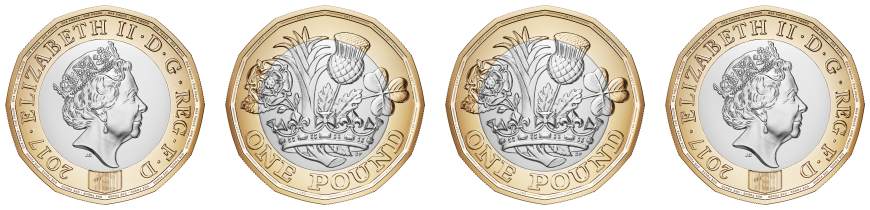
\includegraphics[width=0.4\linewidth]{Chapter1/coinflip.png}
\vspace{-1em}
\end{figure*}
\begin{center}
head, tail, tail, head.
\end{center}

Maybe you would say ``the coin is fair''.  But why, and how \emph{confident} you are in your answer? Furthermore, if I offered you a bet on the next outcome of a coin flip, at what odds would you take that bet?

A Bayesian statistician can easily answer all of the above questions by following Bayesian decision theory \citep{bishop:prml2006, berger:decision2013}. Before observing the coin flip results, he/she will first determine a \emph{prior belief} on whether the coin is bent or not. Usually this belief is represented by two probability values $P(\text{fair})$ and $P(\text{bent})$ that sum to one. 
%
Then he/she builds a conditional probability -- for example $P( \text{head} | \text{fair} )$ is the probability of the coin flip ``head'' given that the coin is fair -- to describe the \emph{likelihood} of a fair/bent coin given an observation. 
%
After observing some simulation outcomes, he/she will adjust his/her \emph{posterior belief} on the unknown properties of the coin using \emph{Bayes' rule} \citep{bayes:bayes_rule1763, laplace:theorie1820}:

\begin{equation}
P(\text{fair} | \text{coin flip results} ) = \frac{P( \text{coin flip results} | \text{fair}) P(\text{fair})}{ P(\text{coin flip results})}
\label{eq:intro_bayes_rule}
\end{equation}
where in our example, the conditional and marginal probabilities are calculated by simply following the sum rule and product rule of probability:
$$ P( \text{coin flip results} | A) = P( \text{head} | A) P( \text{tail} | A) P( \text{tail} | A) P( \text{head} | A), \quad A \in \{ \text{fair}, \text{bent} \} ,$$
$$ P( \text{coin flip results}) = P( \text{coin flip results} | \text{fair}) P(\text{fair}) + P( \text{coin flip results} | \text{bent}) P(\text{bent}) .$$

The Bayesian statistician can finally answer the question, by picking the one with the largest \emph{posterior probability}, i.e.~the coin is fair if 
$$P(\text{fair} | \text{coin flip results} ) > P(\text{bent} | \text{coin flip results} ),$$
or the coin is bent otherwise. Furthermore, he/she can tell us how confident he/she is, for example ``the posterior probability of the coin being fair is $60\%$, so I am not very confident when saying the coin is fair''. In general, by gathering more coin flip results (more than four simulation outcomes in this case), he/she continues adjusting the posterior belief for a fair/bent coin using Bayes' rule, and becomes more confident about the inferred answer. Having the inference result at hand, he/she can even predict the outcome of a future coin flip experiment, again with an uncertainty estimate, then decide whether he/she should accept the bet as well as the correct odds yielding a positive expected return.

The coin flip problem is just an elementary example of \emph{Bayesian inference}, and in general these principles of inference and decision making apply to many real-world tasks as well. Powered by the rules of probability, Bayesian methods allow us to infer the unknown factors given the observed data, quantify the confidence of the inferred results, and make predictions with calibrated uncertainty estimates that support decision making. Critically, \cite{cox:axioms1946} argued that, reasoning under probability rules is the \emph{only} way to perform coherent inference under uncertainty.\footnote{Also see chapters 1 and 2 in \cite{jaynes:book2003}.} So ideally, Bayesian methods should be applied to any situation where well-calibrated inferences need to be made from data. These include prediction tasks such as classifying cat and dog images, and decision making tasks like determining the next action for a robot.

Despite having many desirable theoretical properties, Bayesian methods are less widely used in many exciting applications of artificial intelligence, especially those powered by deep learning \citep{lecun:deeplearning2015, schmidhuber:deeplearning2015, goodfellow:deeplearning2016} such as the AlphaGo system \citep{silver:alphago2016, silver:alphagozero2017} that defeated human Go champion Ke Jie 3-0.\footnote{\url{https://en.wikipedia.org/wiki/AlphaGo_versus_Ke_Jie}}
%
Although the Bayesian approach maintains a posterior distribution of all possible settings of the unknown factors which is desirable, it also requires computing the marginal probability of the observations (in our example $P(\text{coin flip results})$) that involves evaluating \emph{all} possible settings of the neural network weights. Observing this, a deep learning practitioner might respond that ``it takes \emph{forever} to compute Bayes' rule for my task, so I'd better stick to a point estimate that minimises the training error.'' Two recent trends of deep learning applications make the situation even worse for Bayesian inference: 1) the neural networks employed are getting deeper and wider \citep{he:resnet2016, huang:stochastic_depth2016, huang:dense_net2017}, and 2) a typical dataset for deep learning tasks contains millions (if not billions) of instances \citep{deng:imagenet2009, abu:youtube8m2016}.

%

But still, uncertainty quantification is crucial to achieving better deep learning. First, deep learning models are often over-parameterised, and using a point estimate can easily lead to over-fitting and poor predictive performance. Second, as nowadays deep learning techniques are being incorporated into many systems affecting the quality of human life (e.g.~intelligent personal assistants, machine translation, even intelligence systems supporting autonomous driving and health care), it is crucial to make sure these systems know \emph{how confident the model is when performing decision making}. Also, uncertainty information is essential to solving the exploration-exploitation trade-off, which helps learn a better agent faster in reinforcement learning and robotics applications \citep{deisenroth:pilco2011, mcallister:data_efficientRL2016}. Furthermore, Bayesian methods are the gold standard approaches for data efficiency, which is crucial to build a better prediction system for tasks that usually don't have \emph{enough} labelled cases, and potentially present lots of missing values, e.g.~medical applications.  

Fortunately, if fast and accurate \emph{approximation} schemes could be applied to the quantities that a Bayesian statistician would like to compute, then he/she can still perform (approximate) Bayesian inference and quantify the model uncertainty accordingly. Hence the primal challenge for Bayesian inference today is to design fast and accurate \emph{approximate inference} algorithms for complex systems like neural networks and scale them to large datasets, which will be the main subject of the thesis. But before we delve into the development of such algorithms, in the rest of this introductory chapter I shall introduce the mathematical background for approximate inference, and identify fundamental research questions about this subject.




\ifpdf
    \graphicspath{{Chapter1/Figs/Raster/}{Chapter1/Figs/PDF/}{Chapter1/Figs/}}
\else
    \graphicspath{{Chapter1/Figs/Vector/}{Chapter1/Figs/}}
\fi

% A debate between Frequentist and Bayesian

% Approximate inference: why we should care?
\section{Inference, integration and optimisation}
\label{sec:approx_inference}
Probabilistic modelling starts by defining a distribution of data. For instance, in discriminative supervised learning, one would define a conditional distribution $p(\y | \x, \mparam)$, which is also called the \emph{likelihood function} of $\mparam$. A concrete example for this would interpret $p(\y | \x, \mparam)$ as outputting the probability of a configuration of $\y$ (e.g.~a label or a real value) by transforming the input $\x$ (an image, a sentence, etc.) through a neural network parameterised by $\mparam$. Before observing any real-world data, the parameters $\mparam$ are unknown, but we have a prior belief $p_0(\mparam)$ about what value they might take, e.g.~they should have small $\ell_2$ norm if using a Gaussian prior centred at zero. Then we receive the observations $\data = \{ (\x_n, \y_n) \}_{n=1}^N$, and based on data we want to answer questions on the unknown parameters $\mparam$, for example: given $\data$, what is the most probable value of $\mparam$, and how likely is $\mparam$ to be set to a given value? Answering these questions is precisely the procedure of \emph{inference}: a procedure of deducing unknown properties (in our example the neural network weights) given the observed, or known information. 
%

\subsection{Exact Bayesian inference as integration}
Bayesian statisticians are particularly interested in answering the second question, by computing the \emph{posterior distribution}, or the \emph{posterior belief} of $\mparam$ given $\data$, using Bayes' rule:
\begin{equation}
p(\mparam | \data) = \frac{p(\data | \mparam) p_0(\mparam)}{p(\data)},
\label{eq:chap1_bayes_rule}
\end{equation}
with $p(\data | \mparam) = \prod_{n} p(\y_n | \x_n, \mparam)$ following the i.i.d.~assumption. The elegance of Bayes' rule is that \emph{it separates inference from modelling}. The model -- the prior distribution and the likelihood -- completely determines the posterior distribution, and the only thing left is to \emph{compute} the inference.
%

A closer look at Bayes' rule reveals that the core computation of Bayesian inference is \emph{integration}. Using the sum rule and product rule of probability distributions we have the marginal distribution computed as\footnote{In discrete variable case the integral is calculated w.r.t.~discrete measure, i.e.~summation, which will also be referred as integration in the rest of the thesis.}
$$p(\data) = \int p(\data | \mparam) p_0(\mparam) d\mparam,$$
and if this integral is tractable, then the posterior distribution can be easily computed by (\ref{eq:chap1_bayes_rule}). Moreover, to predict the label $\y^*$ on unseen datum $\x^*$ a Bayesian statistician would compute the \emph{predictive} distribution
\begin{equation}
p(\bm{y}^*|\bm{x}^*, \mathcal{D}) = \int p(\bm{y}^*|\bm{x}^*, \bm{\theta}) p(\bm{\theta}|\mathcal{D}) d\bm{\theta},
\label{eq:chap1_bayesian_inference}
\end{equation}
which again requires solving an integration problem. Even more, since it is hard to visualise the posterior distribution in high dimensions, one would instead look at statistics of the posterior, for example
$$ \text{posterior mean  } \mu = \int \mparam p(\mparam | \data) d \mparam, $$
$$\text{posterior covariance matrix  } \Sigma = \int (\mparam -\mu) (\mparam - \mu)^{\text{T}} p(\mparam | \data) d \mparam,$$
both are integration tasks as well. In summary, many tasks in Bayesian computation can be framed as computing an integral of some function $F(\mparam)$ against the posterior distribution:
\begin{equation}
\int F(\mparam) p(\mparam | \data) d \mparam,
\label{eq:chap1_integral}
\end{equation}
and the goal of this thesis is to study how to perform this integration \emph{pragmatically and efficiently}.

\subsection{Approximate Bayesian inference as optimisation}
\label{sec:chap1_approx_infer}

Having an integration task at hand, the first action I would take is to check my college calculus book with the hope of finding an analytical solution. Unfortunately, for a vast number of integrands and distributions, the integral (\ref{eq:chap1_integral}) does not exhibit an analytical form (or at least people have yet to discover it). This is particularly the case for neural networks: except for some limited special cases,\footnote{e.g.~the prior is Gaussian and the neural network only has one hidden layer with ReLU activation. See \cite{hernandez-lobato:pbp2015} for details.} in general the marginal probability is intractable, let alone the posterior and the predictive distribution.

Instead of finding tractable forms of the integral, many mathematicians have their research careers dedicated to an alternative method: \emph{numerical integration}. Because in a continuous space one could never compute $F(\mparam)p(\mparam | \data)$ at \emph{all} locations then sum them up, instead methods such as discretisation and Monte Carlo are employed. The Monte Carlo idea is particularly interesting in our context: since the integral is computed against a probability distribution, a naive approach would first sample from the posterior $\mparam_k \sim p(\mparam_k | \data)$ then approximate the integral as
\begin{equation}
\int F(\mparam) p(\mparam | \data) \approx \frac{1}{K} \sum_{k=1}^K F(\mparam_k).
\end{equation}
However this simple Monte Carlo approach assumes that the posterior distribution is easy to draw samples from, which is again intractable in most scenarios. Statisticians have applied advanced sampling schemes to (approximately) draw samples from the posterior, including importance sampling, rejection sampling and Markov chain Monte Carlo (MCMC) \citep{gelman:dep2014}. Unfortunately, in high dimensions these methods are likely to require a considerable number of samples (if the random variables are highly correlated), and the simulation time for MCMC can be prohibitively long (e.g.~due to slow mixing).

Now comes the brilliant idea of \emph{approximate inference}: can we find another distribution $q(\mparam)$ that makes the \emph{computation} of the integral $\int F(\mparam) q(\mparam) d\mparam$ comparably easier, and at the same time has minimal \emph{approximation error} to the exact integral we want? Concretely, using the knowledge of the functional form $F$ one can come up with a class of candidate distributions $\mathcal{Q}$, in which integrating $F$ w.r.t.~any $q \in \mathcal{Q}$ has analytical form or can be evaluated quickly with numerical methods. Then the only task here is to obtain the \emph{optimal} $q$ distribution in $\mathcal{Q}$ such that the $q$ integral is the most accurate approximation to the exact one. So in short, \emph{approximate inference} converts the integration problem of (Bayesian) inference into an \emph{optimisation} task. For example, an indirect\footnote{a direct method would consider minimising $\text{error}(\mathbb{E}_{q}[F], \mathbb{E}_p[F]) $, however that involves the exact integral and is mostly intractable.} approach for fitting the $q$ distribution would minimise a distance/divergence/discrepancy measure from the approximation to the exact posterior
\begin{equation}
q^*(\bm{\theta}) = \argmin_{q \in \mathcal{Q}} \mathrm{D}[q(\bm{\theta})||p(\bm{\theta}|\mathcal{D})].
\end{equation}
Note here the measure $\mathrm{D}[ \cdot || \cdot ]$ might not be symmetric. A popular choice for the divergence measure is the \emph{Kullback-Leibler divergence} \citep{kullback:divergence1951, kullback:information1959} which leads to the widely used \emph{variational inference} algorithm \citep{jordan:vi1999, ghahramani:variational2000, beal:vi2003}. 
%
In general an optimisation objective function $\mathcal{F}$ is designed to allow an accurate approximation to be obtained:
\begin{equation}
q^*(\bm{\theta}) = \argmin_{q \in \mathcal{Q}} \mathcal{F}(q(\bm{\theta}); p(\bm{\theta}|\mathcal{D})),
\end{equation}
which might not reflect a specific choice of divergence/discrepancy. Often this objective function $\mathcal{F}$ is crafted such that at the optimum, $\mathcal{F}^*$ can serve as an accurate approximation to the (log) marginal distribution, or \emph{model evidence} $\log p(\data)$ as well. A prevalent approach in this category considers constrained optimisation of the \emph{Bethe free energy} \citep{bethe:energy1935} that was first studied in statistical physics, which has also been shown as the underlying objective of another popular approach called \emph{belief propagation} \citep{pearl:bp1982}. All these methods are thoroughly discussed in Chapter \ref{chap:background}. Once $q$ is obtained, at prediction time the Bayesian predictive distribution (\ref{eq:chap1_bayesian_inference}) is approximated by 
\begin{equation}
p(\bm{y}^*|\bm{x}^*, \mathcal{D}) \approx \int p(\bm{y}^*|\bm{x}^*, \bm{\theta}) q(\mparam) d\bm{\theta}.
\label{eq:chap1_approx_predictive_distribution}
\end{equation}
Other interesting quantities to be computed include the (approximated) \emph{Bayesian averaged prediction} $\y^*_{\text{avg}} = \mathbb{E}_{q}[\text{NN}_{\mparam}(\x^*)]$ if $p(\bm{y}^*|\bm{x}^*, \bm{\theta})$ is defined by a neural network $\y^*_{\text{pred}} = \text{NN}_{\mparam}(\x^*)$ that is parametrised by $\mparam$.

\vspace{1em}
\begin{tcolorbox}
\textbf{Remark} (other inference methods)\textbf{.}
Not all statisticians and engineers agree with the Bayesian modelling paradigm. For example, in deep learning a dominating method for training neural networks is \emph{loss function minimisation}, which first defines a loss function $\ell(\y, \hat{\y})$ between the true label $\y$ and the prediction $\hat{\y} = \text{NN}_{\mparam}(\x)$, then minimises the averaged loss computed on the dataset $\data$. Under fairly mild conditions we show in Section \ref{sec:chap2_bnn} that this corresponds to a \emph{maximum likelihood estimation} (MLE) \citep{fisher:mle1922} of the unknown parameters $\mparam$, which puts a uniform prior (which can be improper) on the weights $\mparam$. Also in many cases, adding regularisations such as the $\ell_2$ or $\ell_1$ regularisers corresponds to defining a prior distribution on $\mparam$, which turns the optimisation into a \emph{maximum a posteriori} (MAP) problem. Both cases can be framed in the variational inference framework with the $q$ distribution as a Dirac delta function.
\end{tcolorbox}

\vspace{1em}
\begin{tcolorbox}
\textbf{Remark} (direct approximations to the predictive distribution)\textbf{.}
For Bayesian neural networks (introduced later) people are often more interested in the predictive distribution $p(\y^* | \x^*, \data)$. Indeed, \cite{snelson:compact2005} and \cite{korattikara:dark2015} considered training a parametric model $\hat{p}(\y| \x, \vparam)$ to form a direct approximation to $p(\y^* | \x^*, \data)$, where $p(\y^* | \x^*, \data)$ is (approximately) computed with a carefully tuned MCMC sampler. The approximation is done by \emph{distillation} \citep{hinton:distil2015}, which means the training data for the ``student model'' $\hat{p}(\y| \x, \vparam)$ is generated from the ``teacher model'' $p(\y^* | \x^*, \data)$. Although this approximation is arguably more direct, with an explicit approximation $q(\mparam) \approx p(\mparam | \data)$ one can perform many (approximate) integration tasks with different $F(\mparam)$ functions at the same time.
\end{tcolorbox}

\vspace{1em}
\begin{tcolorbox}
\textbf{Remark} (a comparison to Bayesian quadrature)\textbf{.}
Another important technique for approximating integrals is \emph{Bayesian quadrature} \citep{ohagan:bayesian_quadrature1991, kennedy:bq1996, ghahramani:bayesianMC2003}, which has attracted a lot of attention as well and has been expanded to form part of an emerging research field called \emph{probabilistic numerics}.\footnote{\url{http://www.probabilistic-numerics.org/}} Here we note that, Bayesian quadrature and the approximate inference methods discussed above, address different intractability issues in integration tasks. Typically, Bayesian quadrature assumes the analytical form of the function $F$ is unknown or very expensive to evaluate, and builds a probabilistic model (e.g.~Gaussian process) for $F$ given samples from the target distribution $p$. Approximate inference, on the other hand, constructs approximate distributions to the intractable distribution $p$, and considers tractable functions $F$ instead. In short, both approaches can be categorised as \emph{model-based approximate integration}, with the only difference that they fit approximations to different components of the integrand. Readers are also referred to e.g.~approximate Bayesian computation \citep{beaumont:abc2002} for those integrands without tractable $F$ and $p$, and in this thesis we only study approximate inference methods and assume $F$ is analytic and cheap to compute for a given configuration.
\end{tcolorbox}


% The appealing aspects of black-box methods
\section{Questions to be answered for algorithmic design}
We have just introduced the concept of approximate inference, but in a very vague way. Precisely what does an ``accurate approximation'' look like? In which sense can we claim the designed method is ``computationally easier'' than the exact integration problem?
%
In general we need to answer the following questions when developing new variants of approximate inference algorithms:

\begin{itemize}
	\item[Q1] What is the measure of ``accuracy''? \\
	It is crucial to define the accuracy measure for the specific tasks that approximate inference is applied to. For example Alice might care about the accuracy in terms of the (approximated) predictive likelihood (\ref{eq:chap1_approx_predictive_distribution}), but instead Bob might want an accurate approximation to the model evidence $\log p(\data)$ for model selection and/or hyper-parameter optimisation. Unfortunately, no approximate inference algorithm can provide satisfactory answers for any possible accuracy measure, hence users are encouraged to think about what they really want from an approximation procedure. In the rest of the thesis we answer this question by considering the (approximate) predictive likelihood, predictive error and the log marginal likelihood $\log p(\mathcal{D})$ ($\log p(\bm{x})$ in latent variable model settings) computed using the obtained approximate posterior. 
	
	\item[Q2] Which optimisation procedure/objective function should be used? \\
	Ideally we should directly minimise the error of approximation according to the choice of accuracy measure. For example, if the answer to Q1 is to obtain an approximate posterior with minimal error measure by a selected divergence, then minimising that divergence is arguably ``the correct thing to do'', and it would return the exact answer if the exact posterior is contained in the candidate distribution set $\mathcal{Q}$. However such a desired measure might be intractable to minimise, and most of the time we are forced to select an alternative, or a \emph{surrogate} energy function due to tractability concerns. Hence Q2 can be rephrased as, given a set of ``tractable'' optimisation methods, how do we choose the best one of them such that an ``accurate'' (as defined in Q1) approximation could be obtained?
	
	\item[Q3] What does ``computational efficiency'' mean here? What constraints are present? \\
	As discussed in Section \ref{sec:chap1_approx_infer}, we resort to approximation because 1) analytical solutions are unavailable and 2) the computational resource is limited to perform numerical integration directly. The latter computational constraints include: 
	\begin{itemize}
	\item \emph{low time complexity} required by large-scale inference tasks or online algorithms that needs real-time inference; 
	\item \emph{low space complexity} that is crucial for the ``big data, big model'' settings (typically the case for deep learning);
	\item and \emph{algorithmic tractability} that simply requires the objective function/gradients/fixed point equations to be computable in a fast way, as these are sub-routines in the optimisation procedure.
	\end{itemize}
	 Another practical concern might be, to what extent the designed algorithm could be incorporated into existing infrastructure, with minimal adjustment. For example, deep learning systems prefer gradient-based methods over fixed-point iterative updates, so that we should arguably prioritise gradient descent when designing approximate inference algorithms for them. These constraints are incorporated to the selection of both the inference algorithm and the approximate distribution family $Q$.
	
\end{itemize}

In principle, Q2 and Q3 should be addressed together. For example, new variational objectives are required when the approximate distribution contains mixture components \citep{jaakkola:gmm1998, salimans:mcmcvi2015, tran:vgp2016, ranganath:hvm2016, maaloe:agdm2016}. In other words, the ``tractability'' in Q2 is mainly defined by the answers to Q3. But in many cases people simply select a widely used approximate inference method (e.g. variational inference) which eventually adds the \emph{algorithmic} tractability constraints, and focus more on the design of approximate distributions. One of the main topics studied in this thesis is to remove as many as possible of these algorithmic restrictions, with the hope of enabling very flexible $q$ distributions to be used for better inference results.




% thesis outline
\section{Thesis outline}
The rest of the thesis is organised in two themes (or two parts):

\begin{itemize}
\item[I] Understanding existing research: unifying variational methods. \\
This part of the thesis focuses on the optimisation procedures of existing approximate inference methods, and proposes generalised algorithms that provide unifying views. Chapter \ref{chap:background} summarises existing literature on popular approximate inference algorithms and applications. Then in Chapters \ref{chap:factor_tying} and \ref{chap:vrbound}, two unifying views of variational methods will be presented from different perspectives, in order to both provide a comprehensive understanding and enable wider applications to Bayesian deep learning.

\item[II] Proposing a new research direction: wild approximate inference. \\
In this theme the focus turns to the discussion of approximate inference algorithms that suit complex approximations. In Chapter \ref{chap:wild} I will revisit the principles of approximate inference again, and discuss the importance of developing new approximate inference methods that allow the use of \emph{implicit} approximations or implicit sampling procedures. In Chapter \ref{chap:grad_approx} I will demonstrate with a concrete example how we can train this type of approximation, and demonstrate how this technique enables new applications of approximate inference such as to meta-learning.
\end{itemize} 

Finally Chapter \ref{chap:conclusion} concludes the thesis and discusses future directions of research.

To make the presentation concise I will move all derivation and proof details into Appendix \ref{chap:proofs} (except those are crucial to the presentation). Optional materials for further reading are also included in Appendix \ref{chap:optional}. Additional comments and discussions are also presented as ``remark'' paragraphs just as readers might have seen in previous pages. All these materials can be safely skipped for first reading.

%\vspace{3em}
%{\Large
%\noindent \hrulefill \hspace{0.2cm} \raisebox{-4pt}[10pt][10pt]{\decofourleft ~  \decosix ~ \decofourright} \hspace{0.1cm} \hrulefill
%\vspace{2em}
%}
%
%Approximate inference is a huge topic, and this thesis must have overlooked many important developments and provoking thoughts in the literature. For interested readers I also provide some extra materials that explain those topics in detail. You are more than welcome to check out the following webpage, and your feedback would be much appreciated.
%
%\vspace{1em}
%\begin{center}
%\url{http://yingzhenli.net/home/en/approximateinference}
%\end{center}
\part{Unifying Variational Methods}
%*******************************************************************************
%****************************** Second Chapter *********************************
%*******************************************************************************

\chapter{Divergences, Algorithms and Applications}
\label{chap:background}

\ifpdf
    \graphicspath{{Chapter2/Figs/Raster/}{Chapter2/Figs/PDF/}{Chapter2/Figs/}}
\else
    \graphicspath{{Chapter2/Figs/Vector/}{Chapter2/Figs/}}
\fi

To kickstart the discussion of variational methods unification, I provide a condensed introduction to two classes of well-known approximate inference techniques. I will first start by discussing statistical divergence measures since both of them are closely related to divergence minimisation. Then I will review the two methods in detail. Finally, I will touch on two main learning tasks in Bayesian deep learning as the primary applications of the approaches developed in this thesis.

\section{Statistical divergences for probability distributions}
Many approximate inference algorithms measure the approximation quality by considering the ``closeness'' between the target and the approximation. In this thesis, we will mainly focus on the case where both the target and the approximation are expressed by probability distributions. Then the concept of ``closeness'' is established as \emph{divergence}. Before introducing the formal definition, we briefly discuss the definition of the \emph{probability density function} (PDF)\footnote{For discrete case we refer PDF as probability \emph{mass} functions (PMF).} as preparation. 

Denote the measurable space as $(\Theta, \Sigma)$, where $\Theta$ is the sample space of the random variable $\mparam$ of interest, and $\Sigma$ is a pre-defined $\sigma$-algebra on $\Theta$. A \emph{probability distribution} $P$ is a measure defined on $\Sigma$ such that $P(\Theta) = 1$. Also we assume there exists a dominating measure (also called reference measure) $\mu$ on $\Sigma$ such that, for a probability distribution $P$ in interest which is defined on $\Sigma$, we can define its \emph{probability density function} $p$ by $dP = pd\mu$.\footnote{We can also define divergences without assuming a common reference measure, which is out of the scope of this thesis. In this case one should work with equalities up to zero measure.}
%
For simplicity in the rest of the thesis we will work with the sample space $\Theta = \mathbb{R}^D$, the $\sigma$-algebra $\Sigma = \{ S: S \subset \mathbb{R}^D \}$, and the dominating measure $d\mu = d\mparam$. Finally we write $\mathcal{P}$ the space of PDFs such that any probability distribution $P$ defined on $\Sigma$ has its PDF $p \in \mathcal{P}$.

With all the preparation above we now provide a formal definition of divergence.
\begin{definition}
(Divergence)
Given a set of probability density functions $\mathcal{P}$ for a random variable $\mparam$, a divergence on $\mathcal{P}$ is defined as a function $\mathrm{D}[\cdot || \cdot]: \mathcal{P} \times \mathcal{P} \rightarrow \mathbb{R}$ such that $\mathcal{D}[p||q] \geq 0$ for all $p, q \in \mathcal{P}$, and $\mathcal{D}[p||q] = 0$ iff.~$p = q$. 
\end{definition}
%
This definition is much weaker than that for a \emph{distance} such as the $l_2$-norm, since it does not need to satisfy either symmetry in arguments or the triangle inequality. Hence there exist many available divergences to use, and in this section we review some of the popular choices. We start from the well-known Kullback-Leibler (KL) divergence and discuss its properties and applications. Then we move to a more general case and review $\alpha$-divergences which will be the main divergence tools for the algorithms developed in the first part of the thesis. In Appendix \ref{sec:appendix_other_divergence} we also briefly touch on two very general cases, $f$-divergence and Bregman divergence, and discuss their connections to $\alpha$-divergences.

\subsection{Kullback-Leibler (KL) divergence}
\label{sec:chap2_kl_divergence}
\emph{Kullback-Leibler divergence} \citep{kullback:divergence1951, kullback:information1959}, or \emph{KL divergence}, is arguably one of the most widely used divergence measures, not only in approximate inference but also in machine learning, statistics, and information theory. 
%
\begin{definition}
(Kullback-Leibler Divergence)
The Kullback-Leibler (KL) divergence on $\mathcal{P}$ is defined as a function $\mathrm{KL}[\cdot || \cdot]: \mathcal{P} \times \mathcal{P} \rightarrow \mathbb{R}$ with the following form
\begin{equation}
\mathrm{KL}[p||q] = \int p(\mparam) \log \frac{p(\mparam)}{q(\mparam)} d\mparam, \quad p, q \in \mathcal{P},
\label{eq:chap2_kl_divergence}
\end{equation}
where $\log$ is the natural logarithm (to base $e$).
\label{def:chap2_kl_divergence}
\end{definition}
One can easily check that indeed the above definition is a valid divergence. By Jensen's inequality (see Appendix \ref{sec:appendix_identities}) we have (\ref{eq:chap2_kl_divergence}) always non-negative, and it reaches zero iff.~$p = q$. Also it is clear that the KL divergence is asymmetric, i.e.~$\mathrm{KL}[p||q] \neq \mathrm{KL}[q||p]$. 
%
Historically, especially when used in approximate inference context, these two cases have been referred as the \emph{inclusive} KL divergence for $\mathrm{KL}[p||q]$, and the \emph{exclusive} KL divergence for $\mathrm{KL}[q||p]$. These names originate from the observation that fitting $q$ to $p$ by minimising these two KL divergences returns results of different behaviour, detailed as follows:
%
\begin{itemize}
\item Fitting $q$ to $p$ by minimising $\mathrm{KL}[q||p]$: \\
This KL divergence would emphasise assignment of \emph{low} probability mass of $q$ to the location where $p$ is very small, thus the name ``exclusive'' KL. Consider a region $S \in \Theta$ that has $q(\mparam) > 0$ but $p(\mparam) = 0$ for $\mparam \in S$, then this would make the integrand in (\ref{eq:chap2_kl_divergence}) infinity, thus the KL divergence assigns an extremely high cost to $q$ here. On the other hand, if $p(\mparam) > 0$ but $q(\mparam) = 0$, then the integrand restricted to the subset $S$ is zero, meaning that the cost for missing a region with positive $p$ mass is much lower. We also refer this property as ``zero-forcing'', or ``mode-seeking'' when $q$ is restricted to be uni-modal.

\item Fitting $q$ to $p$ by minimising $\mathrm{KL}[p||q]$: \\
Conversely, this KL divergence would emphasise assignment of \emph{high} probability mass of $q$ to the location where $p$ has positive mass, thus the name ``inclusive'' KL. Consider the case that $q(\mparam) > 0$ but $p(\mparam) = 0$, then this would make the integrand in (\ref{eq:chap2_kl_divergence}) zero. In contrast, if $p(\mparam) > 0$ but $q(\mparam) = 0$, then the integrand is infinity, meaning that the cost for missing a region with positive $p$ mass is extremely high. We also refer this property as ``mass-covering''.

\end{itemize}

Later we will see how these two KL divergences have been applied to approximate inference algorithms such as the widely used variational inference \citep{jordan:vi1999, beal:vi2003} and expectation propagation \citep{minka:ep2001}. But here we switch the topic to maximum likelihood estimation (MLE) \citep{fisher:mle1922} for a moment, in which we will show that MLE is also equivalent to minimising a KL divergence. For a given dataset $\data = \{\x_1, ..., \x_N \}$, define the empirical distribution as $\hat{p}_{\data}(\bm{x}) = \frac{1}{N} \sum_{n=1}^{N} \delta(\x - \x_n)$ where $\delta(\cdot)$ denotes the Dirac delta function. Then we want to fit the data with a parametric probabilistic model $p(\bm{x}|\mparam)$ using MLE:
\begin{equation}
\hat{\mparam}^{\text{ML}} = \argmax_{\mparam \in \Theta} \frac{1}{N} \sum_{n=1}^{N} \log p(\bm{x}_n | \mparam).
\end{equation}
Simple calculation reveals that maximising the log-likelihood of $\mparam$ is equivalent to minimising the KL divergence
\begin{equation*}
\hat{\mparam}^{\text{ML}} = \argmin_{\mparam \in \Theta} \mathrm{KL}[\hat{p}_{\mathcal{D}}(\bm{x}) || p(\bm{x}| \mparam) ] = \argmin_{\mparam \in \Theta} -\frac{1}{N} \sum_{n=1}^{N} \log p(\bm{x}_n | \mparam) + \text{const}.
\end{equation*}
MLE is widely used in all types of machine learning tasks, e.g.~learning generative models (Section \ref{sec:chap2_dgm}). 


\subsection{Amari's $\alpha$-divergences}
\label{sec:chap2_alpha_divergence}

Besides the KL divergence, do we have other choices of divergences for approximate inference? Certainly there are, and here we review a rich class of them called \emph{$\alpha$-divergences}. Interestingly there exist multiple (slightly) different definitions of $\alpha$-divergences, and in the sequel we will formally introduce the version that will be the focus of this chapter. Before that I provide a short (and possibly incomplete) history for these developments in below.

Just after a year of the proposal of the KL-divergence, statistician Herman Chernoff introduced a test statistic for the likelihood-ratio test \citep{chernoff:alpha1952}, and at the end of the paper, he linked the proposed technique to a divergence measure that is computed by the infimum of an integral. That integral has later been referred as the \emph{Chernoff} $\alpha$-coefficient 
$$\int p(\mparam)^{\alpha} q(\mparam)^{1 - \alpha} d\mparam, \quad \alpha \in (0, 1),$$
which is used in all later variants of $\alpha$-divergences. 

In 1961, mathematician Alfr{\'e}d R{\'e}nyi argued that, by removing the additivity requirement, Shannon entropy can be further generalised to many interesting cases \citep{renyi:divergence1961}. He proposed one of such entropy definitions, and then characterised the induced mutual information and relative entropy measures using his version of $\alpha$-divergence.\footnote{The KL divergence characterises the corresponding mutual information and relative entropy measures for Shannon entropy. } These two quantities are now referred to \emph{R{\'e}nyi entropy} and \emph{R{\'e}nyi divergence}, respectively, and the latter will be employed as the divergence tool in Chapter \ref{chap:vrbound}. Perhaps surprisingly, R{\'e}nyi's definition of $\alpha$-divergence also contains the Chernoff $\alpha$-coefficient, although these two developments are rather independent.

In the 70s-80s of the 20th century, differential geometry was introduced to statistics, e.g.~see \cite{efron:curvature1975, efron:geometry_expfam1978, amari:ig1985}, which studies the geometric properties of the manifold obtained by mapping $\mathcal{P}$ to the parameter space $\Theta$. In particular, researchers were interested in the geometrical properties of \emph{exponential family} distributions (introduced later) and the corresponding divergences that reflect these features. In this context, mathematician Shun-ichi Amari introduced his version of $\alpha$-divergence \citep{amari:geometry1982, amari:ig1985}, by generalising the application of Chernoff $\alpha$-coefficient to $\alpha \in \mathbb{R}$.
\begin{definition}
(Amari's $\alpha$-divergence)
Amari's $\alpha$-divergence $\mathrm{D}_{\alpha}^{A}[\cdot || \cdot]: \mathcal{P} \times \mathcal{P} \rightarrow \mathbb{R}$, parameterised by $\alpha \in \{\alpha :  \mathcal{D}_{\alpha}^{A}[p||q] < +\infty \}$, is defined as
\begin{align}
\mathrm{D}_{\alpha}^{A}[p||q] = \frac{4}{ 1 - \alpha^2 } \left( 1 - \int p(\bm{\theta})^{\frac{1 + \alpha}{2}} q(\bm{\theta})^{\frac{1 - \alpha}{2}} d\bm{\theta}\right), \quad \alpha \neq \pm 1, \\
\mathrm{D}_{1}^{A}[p||q] := \lim_{\alpha \rightarrow 1} \mathrm{D}_{\alpha}^{A}[p||q] = \mathrm{KL}[p||q], \quad \alpha = 1, \\
\mathrm{D}_{-1}^{A}[p||q] := \lim_{\alpha \rightarrow -1} \mathrm{D}_{\alpha}^{A}[p||q] = \mathrm{KL}[q||p], \quad \alpha = -1.
\end{align}
\end{definition}

In Amari's career he used $\alpha$-divergence as a tool to study the geometry of distribution manifolds, and in particular, he claimed in \cite{amari:divergence2009} that his definition is the only divergence that belongs to both the $f$-divergences \citep{csiszar:divergence1963} (related to information theory) and Bregman divergences \citep{bregman:divergence1967} (related to geometry). These properties are not directly related to approximate inference, and we only discuss them in Appendix \ref{sec:appendix_other_divergence}.

\vspace{1em}
\begin{tcolorbox}
\textbf{Remark} (Other $\alpha$-divergence definitions)\textbf{.}
There exist other definitions of $\alpha$-divergence, and some of them are detailed here.
\begin{itemize}
\item R{\'e}nyi's $\alpha$-divergence \citep{renyi:divergence1961} (defined on $\alpha \neq 1, \alpha > 0$):
$$\mathrm{D}_{\alpha}^{R}[p||q] = \frac{1}{\alpha - 1} \log \int p(\bm{\theta})^{\alpha} q(\bm{\theta})^{1 - \alpha} d\bm{\theta}.$$
By continuity in $\alpha$ we can show that $\lim_{\alpha \rightarrow 1} \mathrm{D}_{\alpha}^{R}[p||q] = \mathrm{KL}[p||q]$. We defer the detailed introduction of R{\'e}nyi's definition to Section \ref{sec:chap4_vrbound_renyi_divergence}.
%
\item Tsallis's $\alpha$-divergence \citep{tsallis:divergence1988} (defined on $\alpha \neq 1$):
$$\mathrm{D}_{\alpha}^{T}[p||q] = \frac{1}{\alpha - 1} \left( \int p(\bm{\theta})^{\alpha} q(\bm{\theta})^{1 - \alpha} d\bm{\theta} - 1\right).$$ 
Again by continuity in $\alpha$ we can show that $\lim_{\alpha \rightarrow 1} \mathrm{D}_{\alpha}^{T}[p||q] = \mathrm{KL}[p||q]$. 
%
\end{itemize}

\end{tcolorbox}


\section{Variational inference with KL-divergence}
\label{sec:energy}
% Kullback-Leibler divergence and variational free energy
It seems from the introduction of the divergences above that divergence minimisation is an excellent idea to obtain an accurate approximation to the target distribution, where the measure of ``accuracy'' is also represented by the choice of divergence. However direct divergence minimisation is still intractable, since that involves evaluating the target distribution itself. For example, consider minimising the exclusive KL divergence $\mathrm{KL}[q(\mparam) || p(\mparam| \mathcal{D}) ]$ to obtain the approximate posterior. But we still need to compute $p(\mparam|\mathcal{D})$, and in particular the marginal likelihood $p(\mathcal{D})$ which is intractable. In this section we discuss variational inference (VI) -- a widely used approximate inference algorithm -- which incorporates divergence minimisation in a smart way. To emphasise that the algorithm is applicable to more general cases beyond posterior approximation, we now write the \emph{target distribution} as
\begin{equation*}
p(\mparam) = \frac{1}{Z} p^*(\mparam), 
\end{equation*}
where $p^*(\theta)$ is the \emph{unnormalised} target distribution and $Z = \int p^*(\mparam) d\mparam$ is the \emph{normalising constant} or \emph{partition function}. In the posterior approximation context $p^*(\mparam) = p(\mparam, \mathcal{D})$ and $Z = p(\mathcal{D})$.

\subsection{Kullback-Leibler divergence and variational free-energy}

As already discussed, the exclusive KL divergence minimisation problem is intractable. Fortunately the minimiser of the exclusive KL can also be obtained by an equivalent minimisation problem of the so called \emph{variational free-energy} (VFE):
$$ \argmin_{q} \mathrm{KL}[q(\mparam)||p(\mparam)] = \argmin_{q} \mathcal{F}_{\text{VFE}}(q; p),$$
\begin{equation}
\mathcal{F}_{\text{VFE}}(q; p) := \mathrm{KL}[q(\mparam)||p(\mparam)] - \log Z = \int q(\mparam) \log \frac{q(\mparam)}{p^*(\mparam)} d\mparam.
\label{eq:chap2_vfe}
\end{equation}
%
This is because the normalising constant $Z$ is independent with the approximation $q$, thus can be dropped in the exclusive KL. Historically the negative of the variational free-energy is also frequently discussed, which is named \emph{variational lower-bound} or \emph{evidence lower-bound (ELBO)} in the context of posterior approximation
\begin{equation}
\mathcal{L}_{\text{VI}}(q; p) := - \mathcal{F}_{\text{VFE}}(q; p) = \int q(\mparam) \log \frac{p^*(\mparam)}{q(\mparam)} d\mparam.
\label{eq:chap2_vi_lowerbound}
\end{equation}
In posterior inference context (i.e.~$p^*(\mparam) = p(\data, \mparam) = p(\data | \mparam) p_0(\mparam)$) the following two formulations of the variational lower-bound have also been considered:
\begin{equation}
\mathcal{L}_{\text{VI}}(q; p) = \mathbb{E}_q[\log p(\data | \mparam)] - \mathrm{KL}[q(\mparam) || p_0(\mparam) ],
\end{equation}
%
\begin{equation}
\mathcal{L}_{\text{VI}}(q; p) = \mathbb{E}_q[\log p(\data, \mparam)] + \mathbb{H}[q(\mparam)].
\end{equation}
where $\mathbb{H}[q(\mparam)]$ is the Shannon entropy of the $q$ distribution.

The lower-bound property comes from the fact that $\log Z \geq \mathcal{L}_{\text{VI}}(q; p)$, because of the non-negativity of KL divergence. Equivalently, this property can also be derived as follows: 
%
\begin{equation*}
\begin{aligned}
\log Z &= \log \int p^*(\mparam) d \mparam \\
&= \log \int q(\mparam) \frac{p^*(\mparam)}{q(\mparam)} d \mparam \\
&\geq \int q(\mparam) \log \frac{p^*(\mparam)}{q(\mparam)} d \mparam. \quad\quad \text{(Jensen's inequality)}
\end{aligned}
\end{equation*}
Here Jensen's inequality (see appendix \ref{sec:appendix_identities}) is applied to the logarithm which is concave.
%
When posterior approximation is considered we also denote the two quantities as $\mathcal{F}_{\text{VFE}}(q; \mathcal{D})$ and $\mathcal{L}_{\text{VI}}(q; \mathcal{D})$, respectively. 
%
In summary, variational inference finds an approximation to the posterior through an \emph{optimisation} process, which is drastically different from sampling approaches that construct \emph{empirical point mass} distributions to describe the posterior.

\subsubsection{A brief history of variational inference}
Variational inference can be viewed as an application of \emph{variational methods} that mathematicians and physicists have studied for centuries. Historically, physicists mainly focused on mean-field theories for complex systems \citep{parisi:book1988},  whereas \cite{dempster:em1977} as statisticians proposed the famous \emph{expectation maximisation} (EM) algorithm that also has a VI interpretation \citep{neal:em1998}. Interestingly the pioneers of deep learning had also applied variational inference (though under other names) to Bayesian neural networks \citep{peterson:mean_field1987, hinton:mdl1993} that will be surveyed in the application section. Especially since the development of \citet{peterson:mean_field1987}, mean-field approximation started to be an attractive alternative to sampling methods for probabilistic inference in graphical models \citep{ghahramani:em_factorial1995, mackay:ensemblelearning1997}.

However it was until \cite{saul:mean_field1996} which introduced the generic form of the variational lower-bound to explain the mean-field approximation. The first papers that I can find which coined the term ``variational inference'' are \cite{lawrence:vi1998} and \cite{jordan:vi1999}, where \cite{jordan:vi1999} provided a detailed summary of the previous work coming from the same group. Later on, researchers started to extend the variational principle to cases beyond graphical models, e.g.~the \emph{variational Bayes} (VB) algorithm \citep{attias:vb1999, attias:vb2000, ghahramani:variational2000, sato:vb2001, ghahramani:propagation2001, beal:vi2003} that is used to perform posterior approximations of the model parameters and even model selection.




\subsection{A mean-field approximation example}
\label{sec:chap2_mean_field_vi}
As an example for the variational inference algorithm, here we present the variational mean-field approximation \citep{parisi:book1988} for Bayesian linear regression. Readers are also referred to \citet{bishop:prml2006} for more details and here we would briefly cover the derivations presented there. Mean-field approximation, also known as the factorised approximation, assumes the approximate posterior to be the form of
\begin{equation}
q(\mparam) := \prod_{i=1}^{D} q_i(\theta_i).
\label{eq:chap2_mean_field}
\end{equation}
In general one can partition the elements of $\mparam = (\theta_1, \theta_2, ..., \theta_D)$ into disjoint groups and apply factorisations over groups. This general case is usually called \emph{structured} mean-field approximation \citep{saul:structured1996}, and for simplicity in the following example we only consider the fully factorised case (\ref{eq:chap2_mean_field}). Also we emphasise that there's no further assumption/restriction that is made on the functional form of $q_i(\theta_i)$. As we shall see, the variational free-energy is still convex in $q_i(\theta_i)$ and thus the solution provided by the following is the global optimum.

To derive the best approximation in the mean-field distribution family, we first substitute (\ref{eq:chap2_mean_field}) into (\ref{eq:chap2_vfe}) (and use $\mparam_{\neq j}$ to denote all the $\theta_i$ variables except $\theta_j$):
\begin{equation*}
\begin{aligned}
\mathcal{F}_{\text{VFE}}(q; p) &=  \int \prod_i q_i(\theta_i)  \left( \sum_{i} \log q_i(\theta_i) - \log p^*(\mparam)  \right) d\mparam \\
&= \int q_j(\theta_j) \log q_j(\theta_j) d\theta_j  - \int q_j(\theta_j) \left( \int \prod_{i \neq j} q_i(\theta_i)  \log p^*(\mparam) d\mparam_{\neq j} \right) d\theta_j + \text{const}\\
&:=  \int q_j(\theta_j) \log q_j(\theta_j) d\theta_j  - \int q_j(\theta_j) \log \tilde{p}(\theta_j) d\theta_j + \text{const},
\end{aligned}
\end{equation*}
where $\tilde{p}(\theta_j)$ denote the ``marginal'' distribution satisfying
\begin{equation*}
\log \tilde{p}(\theta_j) = \int \prod_{i \neq j} q_i(\theta_i) \log p^*(\mparam) d\mparam_{\neq j} + \text{const}.
\end{equation*}
This means, by fixing the functional form of $q_i$ for all $i \neq j$, VFE is reduced to the KL-divergence $\mathrm{KL}[q_j(\theta_j)||\tilde{p}(\theta_j)]$ plus a constant that is independent to $q_j(\theta_j)$. Thus the free-energy is still convex in $q_j(\theta_j)$, in which the unique global optimum is obtained by setting $q_j(\theta_j) = \tilde{p}(\theta_j)$. To be precise, we explicitly write down the optimal mean-field approximation as
\begin{equation}
q_j(\theta_j) = \frac{ \exp \left[ \int \prod_{i \neq j} q_i(\theta_i)  \log p^*(\mparam) d\mparam_{\neq j} \right] }{ \int \exp \left[ \int \prod_{i \neq j} q_i(\theta_i)  \log p^*(\mparam) d\mparam_{\neq j} \right] d\theta_j}.
\label{eq:chap2_mean_field_opt}
\end{equation}
%
Now as an example consider Bayesian linear regression with 2-D inputs $\bm{x}$ and 1-D output $y$:
\begin{equation*}
\mparam \sim \mathcal{N}(\mparam; \bm{\mu}_0, \bm{\Lambda}_0^{-1}), \quad 
y|\bm{x} \sim \mathcal{N}(y; \mparam^T \bm{x}, \sigma^2).
\end{equation*}
Given the observations $\data = \{ (\bm{x}_n, y_n) \}_{n=1}^N$, the posterior distribution of $\mparam$ can be computed analytically as $p(\mparam|\mathcal{D}) = \mathcal{N}(\mparam; \bm{\mu}, \bm{\Lambda}^{-1})$ with $\bm{\Lambda} = \bm{\Lambda}_0 + \frac{1}{\sigma^2} \sum_n \bm{x}_n \bm{x}_n^T$ and $\bm{\Lambda} \bm{\mu} = \bm{\Lambda}_0 \bm{\mu}_0 + \frac{1}{\sigma^2} \sum_n y_n \bm{x}_n$. To see how the mean-field approach works, we explicitly write down the elements of the posterior parameters
\begin{equation*}
\bm{\mu} = \begin{pmatrix} \mu_1 \\ \mu_2 \end{pmatrix}, \quad
\bm{\Lambda} = \begin{pmatrix} \Lambda_{11} & \Lambda_{12} \\ \Lambda_{21} & \Lambda_{22} \end{pmatrix}, 
\quad \Lambda_{12} = \Lambda_{21},
\end{equation*}
Then by explicitly expanding the mean-field solution (\ref{eq:chap2_mean_field_opt}):
\begin{equation}
\begin{aligned}
\log q_1(\theta_1) &= \int q_2 \log p(\mparam, \mathcal{D}) d\theta_2 + \text{const} \\
&= \mathbb{E}_{q_2} \left[ -\frac{1}{2} (\theta_1 - \mu_1)^2 \Lambda_{11} - (\theta_1 - \mu_1) \Lambda_{12} (\theta_2 - \mu_2) \right] + \text{const} \\
&= -\frac{1}{2} \theta_1^2 \Lambda_{11} + \theta_1 \mu_1 \Lambda_{11} - \theta_1 \Lambda_{12} (\mathbb{E}_{q_2}[\theta_2] - \mu_2) + \text{const} \\
&:= \log \mathcal{N}(\theta_1; m_1, \lambda^{-1}) + \text{const}
\end{aligned}
\label{eq:chap2_mean_field_linear_regression}
\end{equation}
where the new mean $m_1$ and the precision $\lambda_1$ satisfies
\begin{equation*}
m_1 = \mu_1 - \Lambda_{11}^{-1}\Lambda_{12} (\mathbb{E}_{q_2}[\theta_2] - \mu_2), \quad
\lambda_1 = \Lambda_{11}.
\end{equation*}
It is important to note again that we do not assume the approximation to be a Gaussian distribution in order to obtain the last equation in (\ref{eq:chap2_mean_field_linear_regression}). Rather the Gaussian distribution solution came out from the derivation of the global optimum (\ref{eq:chap2_mean_field_opt}) and the completion of the square form.
%
One can derive the terms $m_2 = \mu_2 - \Lambda_{22}^{-1}\Lambda_{21} (\mathbb{E}_{q_1}[\theta_1] - \mu_1)$ and $\lambda_2 = \Lambda_{22}$ for $q_2$ in the same way, and show that $\bm{m} = \bm{\mu}$ is the only stable fixed point of this iterative update. So we have $q_1(\theta_1) = \mathcal{N}(\theta_1; \mu_1, \Lambda_{11}^{-1})$, and similarly $q_2(\theta_2) = \mathcal{N}(\theta_1; \mu_2, \Lambda_{22}^{-1})$ as the unique global optimum of variational mean-field approximation. A visualisation of the mean-field approximation is provided in Figure \ref{fig:chap2_mean_field}. Note here the variance parameter of $q(\theta_1)$ also correspond to the variance of the conditional distribution $p(\theta_1 | \theta_2, \data)$, which is smaller than the variance of the marginal distribution $p(\theta_1 | \data)$, and therefore mean-field VI under-estimates the posterior uncertainty in this case.


\begin{figure}
\centering
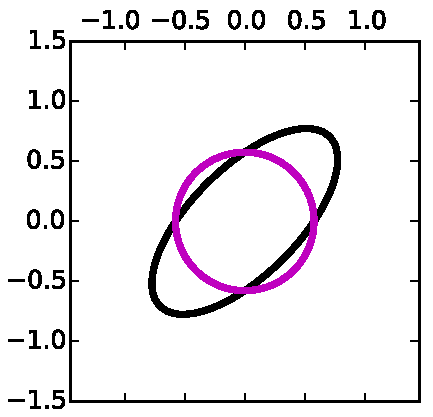
\includegraphics[width=0.25\linewidth]{Chapter2/vi/mean_field.pdf}
\caption{Mean-field approximation to the exact posterior distribution in the Bayesian linear regression example (with one-sigma contours). The exact posterior contour is shown in black and the variational approximation is in purple.}
\label{fig:chap2_mean_field}
\end{figure}



\subsection{Monte Carlo variational inference}
\label{sec:chap2_mcvi}

So far we have discussed variational inference algorithms for linear regression. But real world problems are much more complicated. Often, the term $\mathbb{E}_q[\log p^*(\mparam)]$ in the variational free energy lacks an analytical form. A prevalent example of such cases is variational inference for \emph{large-scale data}: here the unnormalised distribution $p^*(\mparam) := p(\mparam, \data)$ is proportional to the product of many likelihood functions, and evaluating $\mathbb{E}_q[\log p(\data | \mparam)]$ requires a pass of the whole dataset, which can be very expensive. On the other hand, insisting on having an analytical form of the entropy term $\mathbb{H}[q]$ (or $\mathrm{KL}[q||p_0]$) would restrict the selection of $q$ distributions to simple distributions like Gaussians. Usually the exact posterior is very complicated, and these simple distributions are expected to be poor approximations to the target distribution. Hence a key challenge here is, can we design a variational algorithm that applies to complex models, and scales to big data?

One solution to the above request is to develop further approximation techniques \emph{specific to the chosen variational approximation}. Indeed in the early days researchers have attempted to do so, e.g.~see \cite{jaakkola:gmm1998, gershman:nonparametric_vi2012}.  However these solutions are applicable only to a handful of special cases, making them impractical in many other interesting scenarios. Instead in this section we will review another approach which can be quickly applied to many cases with little effort.  It has also been referred as a ``black-box'' approach \citep{ranganath:bbvi2014} due to this feature, but in the rest of the thesis we will refer it as Monte Carlo VI (MC-VI). 

To see how the algorithm works, consider approximating the exact posterior distribution $p(\mparam | \mathcal{D}) \propto \prod_n p(\x_n |\mparam) p_0(\mparam)$ by some simpler distribution $q(\mparam)$. Rewriting the variational lower-bound:
\begin{equation}
\mathcal{L}_{\text{VI}}(q; p) = \sum_{n=1}^N \mathbb{E}_q [\log p(\x_n | \mparam)] + \mathbb{E}_q[\log p_0(\mparam) - \log q(\mparam) ],
\end{equation}
we see that it is the analytical tractability requirement of computing the expectations that restrict the $q$ (and possibly the model $p$) distribution to be of simple form. This constraint can be removed by considering Monte Carlo (MC) approximation to the expectation, which estimates the expectation by, for example
\begin{equation}
\mathbb{E}_{q}[\log p(\x_n|\mparam )] \approx \frac{1}{K} \sum_{k=1}^K \log p(\x_n |\mparam^k ), \quad \mparam^k \sim q(\mparam).
\label{eq:chap2_mc_estimation}
\end{equation}
This forms an \emph{unbiased} estimation, and under mild assumptions (detailed in Chapter \ref{chap:vrbound}), the RHS term in (\ref{eq:chap2_mc_estimation}) converges to the exact expectation value as $K \rightarrow +\infty$. The KL-divergence term in the variational lower-bound can also be estimated with Monte Carlo in a similar manner. Also stochastic optimisation techniques can be extended here for scalability. In summary, with this ``black-box'' approach, one can approximate the variational lower-bound as
\begin{equation}
\mathcal{L}^{\text{MC}}_{\text{VI}}(q; p) = \frac{N}{|\mathcal{S}|} \sum_{n \in \mathcal{S}} \frac{1}{K} \sum_{k} \log p(\x_n | \mparam^k) + \frac{1}{K} \sum_{k} [\log p_0(\mparam^k) - \log q(\mparam^k) ], \quad \mparam^k \sim q(\mparam),
\label{eq:chap2_mcvi}
\end{equation}
and compute stochastic gradient descent on the MC approximation (\ref{eq:chap2_mcvi}) with mini-batch $\mathcal{S} \sim \mathcal{D}^{|\mathcal{S}|}$.

\vspace{1em}
\begin{tcolorbox}
\textbf{Remark} (MC samples for different observations)\textbf{.}
In the MC approximation (\ref{eq:chap2_mcvi}) we assumed using the same set of samples $\{ \mparam^k \}$ to estimate all the expectation terms. In general we can use different sets of samples to do so, for example, for every datapoint $\x_n \in \mathcal{S}$, we can sample different sets of $\mparam^k$ to estimate the associated reconstruction term $\mathbb{E}_{q}[\log p(\x_n | \mparam)]$. Prevalent examples of this approach include stochastic regularisation techniques (SRTs) such as dropout \citep{srivastava:dropout2014, gal:uncertainty2016}.

\end{tcolorbox}

\vspace{1em}
\begin{tcolorbox}
\textbf{Remark} (variance reduction for MC-VI)\textbf{.}
MC-VI relies on stochastic gradient descent/ascent for optimisation, and the gradient of (\ref{eq:chap2_mcvi}) wrt.~the variational parameters $\vparam$ could have very high variance, especially when the latent variable is discrete. Thus recent work has been focused on variance reduction, often employing a pre-computed quantity correlated with the stochastic gradient as a \emph{control variate} \citep{ross:book2002}. Discussions of these methods are out of the scope of the thesis. Interested readers are pointed to e.g.~\citet{paisley:bbvi2012, mnih:nvil2014, gu:muprop2016} for more details.

\end{tcolorbox}

\subsection{Amortised inference}
\label{sec:chap2_amortisation}
So far we have demonstrated how to apply VI to approximate the posterior distribution. However it can still be very slow for running VI on a probabilistic model with lots of unobserved variables, which is typically the case for \emph{latent variable models} -- probabilistic models that have unobserved variables attached to each data instance. For example, a well-known probabilistic model for text data -- latent Dirichlet allocation (LDA) \citep{blei:lda2003}, could involve millions of latent variables when applied to a large corpus. Thus it brings in prohibitive computational burden since each latent variable must have its approximate posterior iteratively refined. Furthermore, for models whose hyper-parameters are updated constantly, the inference procedure is also repeatedly required as a sub-routine. These issues had restricted the extensions of VI to many interesting cases, until the introduction of \emph{amortised inference} that is detailed in below.

Let us start from the mean-field approximation example we had in Section \ref{sec:chap2_mean_field_vi} but with a slightly different set-up. In this case we are interested in learning a latent variable model 
\begin{equation*}
\z_n \sim \mathcal{N}(\z; \bm{\mu}, \bm{\Lambda}^{-1}), \quad y_n | \x_n \sim \mathcal{N}(\y; \z_n^T \x_n, \sigma^2).
\end{equation*}
which is closely related to factor analysis \citep{harman:factor_analysis1976, roweis:linear1999}. In this case the model parameters $\mparam = \{ \bm{\mu}, \bm{\Lambda}, \sigma \}$ are to be learned by approximate maximum likelihood or variational EM, where the variational lower-bound is used as the surrogate loss. In this case we assume for each latent variable $\z_n \in \mathbb{R}^D$ we compute a mean-field approximate posterior $q_n(\z_n) = \prod_{i=1}^D q_n(z_{ni})$, in which we define each factorisation as $q_n(z_{ni}) = \mathcal{N}(z_{ni}; m_{ni}, \lambda_{ni}^{-1})$. 

One strategy to learn these $q$ distributions is to do gradient descent w.r.t.~all the variational parameters $\{ m_{ni}, \lambda_{ni} \}$ until reaching a local optimum. However this approach is inefficient for large-scale data. First, variational parameters must then be maintained for every observed input-output pairs $( \x_n, y_n )$, meaning a space complexity of $\mathcal{O}(ND)$ if $N$ is the total number of observations. Furthermore, when the model parameters are updated, the previously optimal variational parameters are no longer optimal thus requiring loops of gradient descent again. Depending on the changes of the model parameters, the previous optimal solution for the variational parameters might not always be a good initialisation for the current round's optimisation.

Fortunately, observe that in Section \ref{sec:chap2_mean_field_vi} we have the optimal solutions satisfying
\begin{equation*}
\lambda_{ni} = \bm{\Lambda}_{ii} + \frac{1}{\sigma^2} x_{ni}^2, \quad \bm{m}_n = (\bm{\Lambda} + \frac{1}{\sigma^2} \x_n \x_n^T )^{-1} (\bm{\Lambda} \bm{\mu} + \frac{1}{\sigma^2} y_n \x_n),
\end{equation*}
meaning that these optimal variational parameters are functions of the observations $\x_n$ and $y_n$. Hence if we explicitly define the variational parameters as a function of the observations, e.g.~by parameterising $\lambda_{ni} = a_i x_{ni}^{2} + b_i$, and optimise the parameters of these mappings (in our example $a_i$ and $b_i$), then we can drastically reduce the memory cost to $\mathcal{O}(D)$ which is scalable to big data. Furthermore the previous round's solution of $a_i, b_i$ is more likely to be a good initialiser for the current round's optimisation, as the ``local structure'' of $q$ (in our example the quadratic term $x_{ni}^2$) is already encoded in the mapping. In general we will explicitly define the approximate posterior as $q(\z_n | \x_n, y_n)$ to emphasise the dependency on the observations, and only parameterise the ``global structure'' that is shared across all $q$ distributions. 

The above method is termed as \emph{amortised inference} for VI \citep{salimans:reparam2013, kingma:vae2014, rezende:vae2014}, which is:
\begin{itemize}
\item memory efficient, as we only learn the shared information across the approximate posterior distributions for different $(\x_n, y_n, \z_n)$ tuples;
\item faster for training, as the previous round's solution is more likely to initialise the current step well; 
\item generalisable to unseen observations, as the learned variational parameters only capture the global structure of the variational approximation;
\item a good initialisation of $q$ for unseen data, which will then be refined\footnote{Usually amortised inference returns suboptimal approximation to each individual $p(\z_n | \x_n, y_n)$, -- see \citet{cremer:suboptimal2018} for a quantitative analysis -- so refinements upon the amortised distribution are often useful.} by e.g.~VI \citep{marino:vi2018, kim:semi2018} or MCMC \citep{stuhlmuller:inverse2013, hoffman:vae_mcmc2017}.
\end{itemize}
Obviously it also has disadvantages: as the ``global structure'' is typically unknown to the user, a careless design of such amortisation would return distributions with restrictive representation power. One might suggest using neural networks in a way that leads to very flexible $q$ distributions, however the computation of the (MC approximation of the) variational lower-bound requires $\log q(\mparam)$ to be tractable, which is again a very restrictive constraint. Indeed currently neural networks are mostly used to parameterise simple distributions (for example the mean and variance of a Gaussian $q$ distribution), or distributions that are carefully designed using invertible transform \citep{rezende:flow2015, kingma:iaf2016}. Solutions for these problems are further discussed in the second part of the thesis.

\vspace{1em}
\begin{tcolorbox}
\textbf{Remark} (a misconception of amortised inference)\textbf{.}
Amortised inference is sometimes misunderstood as being equivalent to the variational auto-encoder \citep{kingma:vae2014, rezende:vae2014} approach (discussed later) due to the huge popularity of the latter. In fact the general idea goes far beyond: amortisation can be applied to \emph{any} inference technique as long as the optimal solution for it can be described by a mapping from the observed data. 
%
Historically, amortised inference was first developed for non-Bayesian inference schemes. \cite{hinton:ws1995} developed the \emph{wake-sleep} algorithm to train the \emph{Helmholtz machine} \citep{dayan:helmholtz1995}, where the sleep step trains the $q(\z | \x)$ distribution using samples from the model, i.e.~$\z, \x \sim p(\z, \x)$. They also refer $q(\z | \x)$ as the ``recognition model''. \cite{morris:recognition2001} further applied the sleep step update to learn an approximation to the conditional distributions of a directed graphical model. We note that in both cases, there is no guarantee that $q$ approximate the exact posterior well as it never observes real-world data in the sleep step. 
%
In Gaussian process (GP) literature, amortised inference has been applied to GP latent variable models (GPLVMs) to infer the latent variables, under the name ``back constraints'' \citep{lawrence:gp_back_constraint2006}. 
%
Recent progress on amortising (approximate) Bayesian inference includes applications to MAP inference \citep{sonderby:mapsr2016}, importance sampling \citep{burda:iwae2016}, sequential Monte Carlo \citep{paige:smc2016, le:aesmc2017, maddison:fivo2017, naesseth:vsmc2017} and MCMC \citep{li:amcmc2017}. 

\end{tcolorbox}


% EP and power EP
\section{Expectation propagation with $\alpha$-divergences}
This section reviews another important class of approximate inference algorithms: expectation propagation (EP)\citep{minka:ep2001, opper:ec2005}. EP can be viewed as a generalisation of the well-known sum-product algorithm and belief propagation \citep{pearl:bp1982, pearl:book1988} for computing marginal distributions of a probabilistic (graphical) model. Also by generalising EP to minimising alpha-divergences, a broad class of approximate inference algorithms -- including variational inference -- is recovered. 
%
Many topics detailed below can also be founded in \citet{wainwright:graphical2008, koller:pgm2009}.


\subsection{Factor graphs and exponential families}

One way to represent a distribution is to draw a \emph{factor graph} \citep{kschischang:fg1998, kschischang:fg2001}. A simple example would be a joint distribution $P(\bm{x}_1, \bm{x}_2, \bm{x}_3)$ which can be factorised into $P(\bm{x}_1, \bm{x}_2, \bm{x}_3) = f_1(\bm{x}_1) f_2(\bm{x}_2) f_3(\bm{x}_3)$, illustrated in Figure \ref{fig:factor_graph}. To give a formal definition, a factor graph is a bipartite graph between variable nodes (circles) and factor nodes (squares), where a factor node $f$ is connected to a variable node $\bm{x}_i$ iff.~$\bm{x}_i$ belongs to the function $f$'s domain. A distribution may be represented by different factor graphs, since we can merge factors to a single one. In particular to our example, we may also write $P(\bm{x}_1, \bm{x}_2, \bm{x}_3) = f'_1(\bm{x}_1) f'_2(\bm{x}_2, \bm{x}_3)$, where $f'_1(\bm{x}_1) = f_1(\bm{x}_1)$ and $f'_2(\bm{x}_2, \bm{x}_3) = f_2(\bm{x}_2) f_3(\bm{x}_3)$. Factor graphs enable fast marginal computations using the sum-product algorithm, and in later sections we will see that the EP update procedure also depends on the factor graph structure directly. Therefore, factor graphs can also be viewed as ``hyper-parameters'' specified by the user, and selecting the appropriate factorisation is key to both the approximation accuracy and the computational efficiency. For simplicity in the rest of this chapter we assume the selected factorisation suits well for the learning method. To reduce notation clutter we use $\bm{x}_a$ to denote a subset of random variables $\{\bm{x}_i\}$ connected to a factor node $f_a$.

\begin{figure}
\centering
\subfigure[$P(\bm{x}_1, \bm{x}_2, \bm{x}_3) \propto f_1(\bm{x}_1) f_2(\bm{x}_2) f_3(\bm{x}_3)$]{
  % model_lda.tex
%
% Copyright (C) 2010,2011 Laura Dietz
% Copyright (C) 2012 Jaakko Luttinen
%
% This file may be distributed and/or modified
%
% 1. under the LaTeX Project Public License and/or
% 2. under the GNU General Public License.
%
% See the files LICENSE_LPPL and LICENSE_GPL for more details.

% Latent Diriclet allocation model

%\beginpgfgraWcnamed{model-lda}
\begin{tikzpicture}[x=1.7cm,y=1.8cm]

  % Nodes

  \node[latent]                   (X1) at (0, 0)      {$\bm{x}_1$} ; %
  \node[latent]    (X2) at (1, 0)     {$\bm{x}_2$} ; %
  \node[latent]    (X3) at (2, 0)     {$\bm{x}_3$} ; %


  % Factors
  \factor[above=of X1]     {X1-f1}     {above:$f_1$}{}{}%{left:$Q(W, H)$} {} {} ; %
  \factor[above=of X2]     {X2-f2}     {above:$f_2$}{}{}%{left:$Q(W, H)$} {} {} ; %
  \factor[above=of X3]     {X3-f3}     {above:$f_3$}{}{}%{left:$Q(W, H)$} {} {} ; %

  \factoredge[-] {X1}   {X1-f1}   {} ; %
 	\factoredge[-] {X2}    {X2-f2}	{}
  \factoredge[-] {X3}    {X3-f3}	{}

\end{tikzpicture}
%\endpgfgraphicnamed

%%% Local Variables: 
%%% mode: tex-pdf
%%% TeX-master: "example"
%%% End: 
}
\hspace{1.0in}%
\subfigure[$P(\bm{x}_1, \bm{x}_2, \bm{x}_3) \propto f'_1(\bm{x}_1) f'_2(\bm{x}_2, \bm{x}_3)$]{
  % model_lda.tex
%
% Copyright (C) 2010,2011 Laura Dietz
% Copyright (C) 2012 Jaakko Luttinen
%
% This file may be distributed and/or modified
%
% 1. under the LaTeX Project Public License and/or
% 2. under the GNU General Public License.
%
% See the files LICENSE_LPPL and LICENSE_GPL for more details.

% Latent Diriclet allocation model

%\beginpgfgraWcnamed{model-lda}
\begin{tikzpicture}[x=1.7cm,y=1.8cm]

  % Nodes

  \node[latent]                   (X1) at (0, 0)      {$\bm{x}_1$} ; %
  \node[latent]    (X2) at (1, 0)     {$\bm{x}_2$} ; %
  \node[latent]    (X3) at (2, 0)     {$\bm{x}_3$} ; %
  
  \factor[above=of X2]     {X2-f2-X3}     {above:$f'_2$}{}{}%{left:$Q(W, H)$} {} {} ; %


  % Factors
  \factor[above=of X1]     {X1-f1}     {above:$f'_1$}{}{}%{left:$Q(W, H)$} {} {} ; %


  \factoredge[-] {X1}   {X1-f1}   {} ; %
 	\factoredge[-] {X2}    {X2-f2-X3}	{X3}

\end{tikzpicture}
%\endpgfgraphicnamed

%%% Local Variables: 
%%% mode: tex-pdf
%%% TeX-master: "example"
%%% End: 
}
\caption{Two different factor graph representations for the same probability distribution, if defining $f'_1 = f_1$, $f'_2 = f_2 f_3$.}
  \label{fig:factor_graph} %% label for entire figure 
\end{figure} 

\subsubsection{Exponential family distributions}
Another important concept we introduce here is the \emph{exponential family} distribution \citep{koopman:expfam1936}.
%
As a motivating example, consider fitting a probabilistic model $p$ to some empirical distribution $\hat{p}_{\mathcal{D}}$ by matching some statistical quantity $\bm{\Phi}(\mparam)$. There exists infinitely many solutions for this problem, and here we would prefer the solution which has the maximum \emph{entropy} $\mathbb{H}[p] = - \int p(\mparam) \log p(\mparam) d\mparam$. This means the solution produces samples that have the same statistics as the data distribution, but also retains maximal uncertainty (in terms of the entropy). Solving this constrained optimisation algorithm reveals that the optimal fit has an exponential family form as follows.
%
\begin{definition}
(Exponential family)
An exponential family distribution is defined as 
\begin{equation}
p(\mparam) = \frac{1}{Z} h(\mparam) \exp \left[ \bm{\lambda}^{\text{T}} \bm{\Phi} ( \mparam )  \right],
\label{eq:chap2_vi_expfam}
\end{equation}
where $h(\mparam)$ is the base measure, $\bm{\lambda}$ is the natural parameter or canonical parameter, and $\bm{\Phi}(\mparam)$ is the sufficient statistic.
\end{definition}
%
The natural parameter $\bm{\lambda}$ of the maximum entropy solution is selected to satisfy the constraint $\mathbb{E}_p [\bm{\Phi}(\theta)] = \mathbb{E}_{\hat{p}_{\mathcal{D}} } [\bm{\Phi}(\theta)]$. If the exponential family is \emph{regular}, i.e.~the components of $\bm{\Phi}$ are linearly independent, then there exists a one-to-one mapping between the natural parameter and the expectation of the sufficient statistics $\bm{\mu} := \mathbb{E}_{p}[\bm{\Phi}(\mparam)]$. Thus $\bm{\mu}$ is also named \emph{moment parameter} or \emph{mean parameter} of an exponential family distribution. For notational simplicity we also assume the base measure $h(\mparam) = 1$ and the above exponential family is regular. Hence the partition function $Z$ is a function of the natural parameter $\bm{\lambda}$ (and equivalently a function of the moment parameter $\bm{\mu}$ as well) and we will also write $Z = Z(\bm{\lambda}) = Z(\bm{\mu})$ when necessary. 

Here we include some important properties of exponential family distributions \citep{wainwright:graphical2008}, which can be proved by simple calculations.
\begin{prop}
\label{prop:chap2_expfam}
A regular exponential family distribution (\ref{eq:chap2_vi_expfam}) satisfies the following: \\
(1) $\log Z(\bm{\lambda})$ is convex in $\bm{\lambda}$; \\
(2) $\bm{\mu} = \nabla_{\bm{\lambda}} \log Z(\bm{\lambda})$, and $\text{Cov}_{p}[\bm{\Phi}] = \nabla \nabla_{\bm{\lambda}} \log Z(\bm{\lambda})$; \\
(3) The Fenchel dual $(\log Z)^*(\bm{\mu}) = -\mathbb{H}[\bm{\mu}]$, where $\mathbb{H}[\bm{\mu}]$ denotes the entropy of the exponential family distribution (\ref{eq:chap2_vi_expfam}) with moment parameter $\bm{\mu}$.
\label{prop:chap2_vi_expfam}
\end{prop}
%
The last property is particularly interesting in variational inference context. Recall the Fenchel duality equation $\log Z(\bm{\lambda}) = \max_{\bm{\nu}} \bm{\lambda}^{\text{T}} \bm{\nu} + \mathbb{H}[\bm{\nu}]$, where the maximum is obtained at $\bm{\nu}^* = \bm{\mu}$. This means if the target distribution belongs to some complicated exponential family\footnote{Notice that we can also write the target distribution as $p(\mparam) = \frac{1}{Z} \exp \left[ 1 \cdot \log p^*(\mparam) \right]$. } and the $q$ distribution has moments $\bm{\nu}$, then the Fenchel duality equation is exactly the optimisation problem of VI (\ref{eq:chap2_vfe}). In particular, if $q$ also belongs to the same exponential family, then the optimal approximation can be obtained by matching the moments $\bm{\nu} \leftarrow \bm{\mu}$, thus $q = p$. 

\subsection{Expectation propagation}
\label{sec:chap2_ep_algorithm}

Now we consider a distribution $p(\bm{\theta}) \propto \prod_{a} \tilde{f}_a(\bm{\theta}_a)$, where $\tilde{f}_a$ are the factors in the corresponding factor graph with associated variables $\bm{\theta}_a$. A prevalent example for such a distribution is the exact posterior, where now $\tilde{f}_a$ represents either the prior distribution or the likelihood function associated with a datum. The marginal probability of a subset of $\bm{\theta}$ can be complicated. The highly successful Expectation Propagation (EP) \citep{minka:ep2001} algorithm approximates these exact marginals by another factor graph with a collection of simpler functions $q(\bm{\theta}) \propto \prod_{a} f_a(\bm{\theta}_a)$. It iteratively updates the approximating factors $\tilde{f}_a$ through the ``exclusion-moment matching-inclusion'' procedure, detailed in Algorithm \ref{alg:ep_general}.

%
To summarise the algorithm, we first define the ``leave-one-out'', or \emph{cavity distribution}\footnote{The name ``cavity'' comes from the \emph{cavity method} that is used to study Ising models \citep{mezard:spin1987}, again showing the deep connections between EP and belief propagation.}
\begin{equation}
q_{-a} \propto \prod_{b \neq a} f_b(\bm{\theta}_b) \propto q(\bm{\theta}) / f_a(\bm{\theta}_a),  
\end{equation}
which is computed by multiplying all the other factors except the selected one. Also an ordering of this factor selection is called a \emph{schedule} of the EP algorithm, and in the following we assume it is random. The second step is to compute the \emph{tilted distribution} by inserting back the true factor $\tilde{f}_a$ that $f_a$ approximates:
\begin{equation}
\tilde{p}_{a}(\bm{\theta}) \propto q_{-a}(\bm{\theta}) \tilde{f}_a(\bm{\theta}_a),
\end{equation}
and update the selected factor $f_a$ by minimising the KL divergence from $\tilde{p}_{a}$ to the approximation $q$ (with $f_a$ included), with the restriction that the new $q$ belongs to the same family of previous approximation. For exponential family approximations, we solve this optimisation problem by zeroing the gradients of the KL w.r.t.~the natural parameters of $q$. This is equivalent to matching the moments of the arguments between the two distributions. More precisely, assume the factors $f_a$ belong to the same exponential family with feature function $\bm{\Phi}(\bm{\theta}) = (\Phi_1(\bm{\theta}), ..., \Phi_d(\bm{\theta}))$, then we write the $q$ distribution as
\begin{equation}
q(\bm{\theta}) \propto \exp(\bm{\lambda}^{\text{T}} \bm{\Phi}(\bm{\theta})),
\label{eq:chap2_ep_expfam_param}
\end{equation}
where $\bm{\lambda}$ denote the natural parameters. Zeroing the gradient of $\mathrm{KL}[\tilde{p}_{a} || q]$ wrt.~$\bm{\lambda}$ (and viewing $\tilde{p}_{a}$ as constant) returns
\begin{equation}
\mathbb{E}_{q} \left[ \bm{\Phi}(\bm{\theta}) \right] = \mathbb{E}_{\tilde{p}_{a}} \left[ \bm{\Phi}(\bm{\theta}) \right],
\label{eq:chap2_ep_moment_matching}
\end{equation}
%
which gives the name of moment matching \citep{seeger:ep2005}. We denote this optimisation computation with $\mathrm{proj}$ operator
\begin{equation}
\mathrm{proj}[p] = \arg\min_{q} \mathrm{KL}[p|| q],
\end{equation}
which returns the minimiser of the KL-divergence $\mathrm{KL}[\tilde{p}_{a}||q]$ by passing the moments of $\tilde{p}_{a}$. This operator is also called M-projection \citep{cover:itbook1991}. After the computation of $q^* = \mathrm{proj}[\tilde{p}_a]$ we recover the update of $f_a$ by
\begin{equation}
f_a(\bm{\theta}_a) \leftarrow q^*(\bm{\theta}) / q_{-a}(\bm{\theta}).
\end{equation}
%
To improve convergence damping updates can be applied to step 4 in Algorithm \ref{alg:ep_general} as
\begin{equation}
f_a(\bm{\theta}_a) \leftarrow f_a(\bm{\theta}_{a})^{1 - \epsilon} \left(\mathrm{proj}[\tilde{p}_{a}] / q_{-a}(\bm{\theta}) \right)^{\epsilon},
\end{equation}
where $\epsilon$ denotes the step-size. The last step, corresponded to the inclusion step in Algorithm \ref{alg:ep_general}, is to incorporate the updated factor back to the approximation:
\begin{equation}
q(\bm{\theta}) \leftarrow q_{-a}(\bm{\theta}) f_a(\bm{\theta}_a).
\end{equation}
The reader may find that in Algorithm \ref{alg:ep_general} the updated distribution $q$ equals to $q^*$ in the moment matching step, while this yields EP without damping only.

%
\begin{algorithm}[t] 
\caption{Expectation Propagation (without damping)} 
\label{alg:ep_general} 
\begin{algorithmic}[1] 
%\STATE initialize $\{\tilde{f}_a\}$
\WHILE{not converged}
	\STATE choose a factor $f_a(\mparam_a)$ to refine (according to a schedule):
	\STATE exclusion: $q_{-a}(\bm{\theta}) \propto q(\bm{\theta}) / f_a(\bm{\theta}_a)$
	\STATE moment matching: $f_a(\bm{\theta}_a) \leftarrow \mathrm{proj}[q_{-a}(\bm{\theta}) \tilde{f}_a(\bm{\theta}_a)] / q_{-a}(\bm{\theta})$
	\STATE inclusion: $q(\bm{\theta}) \leftarrow q_{-a}(\bm{\theta}) f_a(\bm{\theta}_a)$
\ENDWHILE
%\RETURN $\{\tilde{f}_a\}$
\end{algorithmic}
\end{algorithm}
%


\vspace{1em}
\begin{tcolorbox}
\textbf{Remark} (misconceptions about EP)\textbf{.}
A misleading interpretation states that EP is the counterpart algorithm of VI which minimises the inclusive KL. The correct answer is more than ``yes or no'' and it strongly depends on the factor graph structure.
If the factor graph only contains a single factor node, then EP is minimising the inclusive KL globally. However, computing moments on this factor graph often requires further approximations, thus it is rarely considered in EP literature until the development of Chapter \ref{sec:vrbound_all}. Otherwise, EP does \emph{not} minimise the inclusive KL divergence to the target distribution. Thus we refer EP as a \emph{local approximation} algorithm since it works with the components of the target distribution directly. Conversely, VI does minimise the exclusive KL divergence \emph{globally}, regardless of the factor graph structure.
\end{tcolorbox}

\subsubsection{Why EP works}
%(how to describe the intuition well?)\\
In general, to obtain an accurate approximation for some complicated distribution is a difficult task, as estimating the approximate functions \textit{jointly} is often intractable. Factor graphs provide not only a factorised representation of the true distribution but also a guide for choosing the function families for approximation. Consider the minimisation task $q^* = \argmin_q \mathrm{D}[p || q]$.\footnote{Here the measurement can be any distance or divergence, each returns different benefits. In EP the divergence measure is the KL divergence.} Below we discuss 3 difference methods for the optimisation problem, where we understand them as different schedules.\footnote{This is an explanatory discussion rewritten from my first year report.}

The simplest way is independent factorised approximation, i.e.~to approximate each factor independently. This returns a fast and parallelisable algorithm that a simple map-reduce scheme can be applied to. However, is it common that factors share random variables, in which the marginals of the selected factor's random variables can deviate from that factor's function value. From the nature of product we know that small errors of each factor approximation can easily accumulate to large errors of the final result $q$. 

The statistics and control communities have noted the importance of including the dependence in approximation, resulting in the well-known assumed density filtering (ADF) algorithm \citep{maybeck:adf1982}. It can be viewed as a restricted version of factorised approximation by greedily adding in more factors to the $q$ distribution such that $q(\mparam) f_a(\mparam)$ matches $q(\mparam) \tilde{f}_a(\mparam)$ as close as possible. One simple example would be approximating $p(\mparam) = \tilde{f}_1(\mparam) \tilde{f}_2(\mparam) \tilde{f}_3(\mparam)$ with $q(\mparam) = f_1(\mparam) f_2(\mparam) f_3(\mparam)$. Assume we start from an accurate estimation of $f_1(\mparam) \approx \tilde{f}_1(\mparam)$ (where now $q(\mparam) = f_1(\mparam)$), ADF in current iteration incorporates $f_2(\mparam)$ (or $f_3(\mparam)$ depending on the schedule) to the $q$ distribution, updates $f_2(\mparam)$ such that it minimises $\mathrm{D}[q(\mparam) \tilde{f}_2(\mparam) || q(\mparam) f_2(\mparam)]$,
and includes the new approximation $f_2(\mparam)$ to the new $q(\mparam) \leftarrow f_1(\mparam) f_2(\mparam)$. 
The disadvantage of this approach is its sensitivity to the choice of the schedule, especially when a subset of variables is shared by most of the factors. 

EP tries to address the problem of sensitivity to scheduling by looping through the factors repeatedly, giving a chance for inaccurate factors to ``correct themselves''. This puts further restrictions to the mean-field update by including all the factors in moment matching. The precision may oscillate as the approximation in the first few loops can be very poor, especially considering EP is reduced to ADF in the first iteration if initialising all the approximating factors as 1 (which is often the case). Also there is no guarantee for EP to converge. But EP (and in general message passing) is still an efficient algorithm, especially when applying to only a subset of factors (see the application to error-correcting codes \citep{peterson:ecc1972} and TrueSkill algorithm \citep{herbrich:trueskill2006}). 

\subsubsection{Linking power EP and $\alpha$-divergence}
An extension of EP is power EP \citep{minka:powerep2004}, which excludes a fraction of the approximation (i.e. $f_a(\bm{\theta})^{\alpha}$) and includes the same fraction of the true factor for updates (see Algorithm \ref{alg:powerep_general}). Since we exclude/include only a fraction of the factors, damping should be applied to the natural parameters of $f_a(\bm{\theta})^{\alpha}$ directly before recovering the update for $f_a(\mparam)$.

\begin{algorithm}[t] 
\caption{Power EP with fraction $\alpha$} 
\label{alg:powerep_general} 
\begin{algorithmic}[1] 
%\STATE initialize $\{\tilde{f}_a\}$
\WHILE{not converged}
	\STATE choose a factor $f_a(\mparam_a)$ to refine:
	\STATE exclusion: $q_{-a}(\bm{\theta}) = q(\bm{\theta}) / f_a(\bm{\theta}_a)^{\alpha}$
	\STATE moment matching: $f_a(\bm{\theta}_a)^{\alpha} \leftarrow \mathrm{proj}[q_{-a}(\bm{\theta}) \tilde{f}_a(\bm{\theta}_a)^{\alpha}] / q_{-a}(\bm{\theta})$
	\STATE inclusion: $q(\bm{\theta}) \leftarrow q(\bm{\theta}) f_a(\bm{\theta}_a) / f_a(\bm{\theta}_a)^{old}$
\ENDWHILE
%\RETURN $\{\tilde{f}_a\}$
\end{algorithmic}
\end{algorithm}

Power EP with fraction $\alpha$ corresponds to minimising the $\alpha$-divergence from $\tilde{p}_{a}(\mparam) \propto q(\mparam) \tilde{f}_a(\mparam) / f_a(\mparam)$ to $q(\mparam)$. To see this, we first adapt Amari's definition \citep{amari:ig1985} of $\alpha$-divergence $\mathrm{D}_{\alpha}^{A}$ to the following form \citep{zhu:divergence1995, minka:divergence2005}, which we refer to as Minka's $\alpha$-divergence:
\begin{equation}
 \mathrm{D}_{\alpha}^{M}[p||q] = \frac{1}{\alpha (1 - \alpha)} \left( 1 - \int p(\bm{\theta})^{\alpha} q(\bm{\theta})^{1 - \alpha} d\bm{\theta}\right)\,
\end{equation}
which is equivalent to the original definition by setting $\alpha' = 2 \alpha - 1$ in Amari's notation $\mathrm{D}_{\alpha'}^A = \mathrm{D}_{\alpha}^M$.
%
So similarly the exclusive KL divergence $\mathrm{KL}[q || p] = \lim_{\alpha \rightarrow 0} \mathrm{D}_{\alpha}^M [p || q]$ and the inclusive one $\mathrm{KL}[p || q] = \lim_{\alpha \rightarrow 1} \mathrm{D}_{\alpha}^M [p || q]$ can be recovered. Now we investigate the case which replaces the moment matching step in the EP algorithm (Algorithm \ref{alg:ep_general}) by $q^* = \argmin D_{\alpha}^M[\tilde{p}_{a}||q]$, which is also called $\alpha$-projection \citep{amari:ig2000}. Similarly we assume $q$ has an exponential family form (\ref{eq:chap2_ep_expfam_param}), and we fix $\tilde{p}_{a}(\mparam)$ as the target. Then when $\alpha \neq 0, 1$,
\begin{equation*}
\begin{aligned}
\nabla_{\bm{\lambda}} D_{\alpha}^M[\tilde{p}_{a}||q] &= \frac{1}{\alpha} \left( \mathbb{E}_{q}[\bm{\Phi}(\bm{\theta})] - \mathbb{E}_{\tilde{p}_{a}^{(\alpha)}}[\bm{\Phi}(\bm{\theta})] \right), \\
\tilde{p}_{a}^{(\alpha)} &\propto \tilde{p}_a^{\alpha} q^{1 - \alpha}.
\end{aligned}
\end{equation*}
In this case the solution of $\nabla_{\bm{\lambda}} D_{\alpha}^M[\tilde{p}_{a}||q]$ is non-trivial since now $\tilde{p}_{a}^{(\alpha)}$ contains contributions from $q$. Instead power EP proposes a fixed point iterative update procedure, by initialising $q$ with last iteration's solution (which makes $\tilde{p}_{a}^{(\alpha)} \propto q \tilde{f}_a^{\alpha} / f_a^{\alpha}$, see the moment matching step in Algorithm \ref{alg:powerep_general}), fixing $\tilde{p}_{a}^{(\alpha)}$ as the target, and computing the next update for the natural parameter $\bm{\lambda}$ such that the moments of $q$ and $\tilde{p}_a^{(\alpha)}$ are matched. Again there is no guarantee for convergence here, but if power EP does converge, this means the fixed point iterative updates are also converged, thus the final solution $q$ does minimises Minka's $\alpha$-divergence (or Amari's $\alpha$-divergence but with a different $\alpha$ value) locally. \cite{minka:powerep2004} also sketched an algorithm called $\alpha$-EP which assumes the $\alpha$-projection is tractable.

Different $\alpha$-divergences show different characteristics, and the family includes the two KL-divergences. Variational methods minimise the exclusive KL-divergence and provides a lower bound on model evidence. Furthermore, the exclusive KL-divergence has an unique advantage in that local optimisation can return optima of global approximation. However, Bayesian predictions often require just the marginals, and the inclusive KL-divergence is the only $\alpha$-divergence which preserves them. Hence standard EP is preferred, which searches the optimisers with invariant sufficient statistics locally at $\bm{\theta}_a$. 

To understand how the choice of other $\alpha$ values might affect the result of approximate inference, consider the problem of approximating a complicated distribution $p$ with a tractable Gaussian distribution $q$ by minimizing $\mathrm{D}_{\alpha}^{M}[p||q]$. The resulting (unnormalized) approximations obtained for different values of $\alpha$ are visualized in Figure \ref{fig:alpha_divergence}. This shows that when $\alpha$ is a large positive number the approximation $q$ tends to cover all the modes of $p$, while for $\alpha \rightarrow -\infty$ (assuming the divergence is finite) $q$ is attracted to the mode with the largest probability mass. The optimal setting of $\alpha$ might reasonably be expected to depend on the learning task that is being considered.

\begin{figure}
\centering
 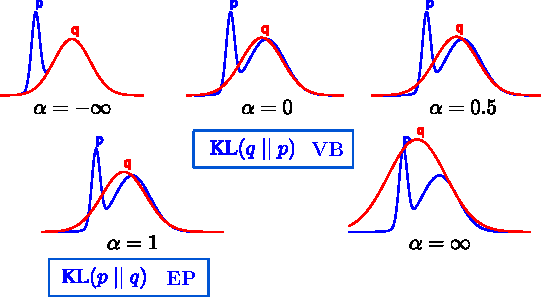
\includegraphics[width=0.7\linewidth]{Chapter3/bbalpha/figs/alpha_divergence}
 \caption{An illustration of approximating distributions by $\alpha$-divergence minimization. Here $p$ and $q$ shown in the graphs are unnormalized probability densities. Reproduced from \citet{minka:divergence2005}. Best viewed in color.}
 \label{fig:alpha_divergence}
\end{figure}

Setting aside the analytic tractability of the computations, we note that the
minimisation of a global $\alpha$-divergence might not always be desirable. If
the true posterior has many modes, then when a Gaussian approximation is deployed, a global approximation of this flavour that
is refined using $\alpha \geq 1$ will cover the modes, and can place
substantial probability in the area where the true posterior has low
probability (see the last plot in Figure \ref{fig:alpha_divergence}). 

\subsection{EP energy: a primal-dual story}
\label{sec:chap2_ep_energy}

EP has been criticised for not having convergence guarantees and instead being a heuristic for posterior approximation. On the other hand, it has been shown to have superior performance compared to VI on a variety of tasks, e.g.~Gaussian Process classification \citep{kuss:gpep2005}. To understand these seemingly contradicting observations, here we provide an energy minimisation view of EP,\footnote{material based on my NIPS 2016 approximate inference workshop abstract, see publication page.} and discuss why EP could potentially lead to better approximations, and why it is difficult to prove the convergence of EP. Similar derivations are also available in \citet{yedidia:bethe2001, heskes:ep2002, minka:divergence2005, opper:ec2005, wainwright:graphical2008}, and some extensions to handling latent variable models are provided in appendix \ref{sec:appendix_relaxation}.

To streamline the notation, we consider approximating the intractable posterior $p(\mparam|\mathcal{D}) = \frac{1}{Z} p_0(\mparam) \prod_{n=1}^N p(\bm{x}_n|\mparam)$ as a running example. In this case we denote $\tilde{f}_n(\mparam) = p(\bm{x}_n|\mparam)$ and leave the prior $p_0(\mparam)$ as it is. Using this notation we again write down the objective function of Variational inference (VI) called the \emph{variational free energy} (VFE) \citep{jordan:vi1999, beal:vi2003}:
\begin{equation}
\min_{q \in \mathcal{Q}} \mathrm{KL}[q||p] \Leftrightarrow \min_{q \in \mathcal{Q}} \mathcal{F}_{\text{VFE}}(q) = \mathbb{E}_{q} \left[ \log q(\mparam) - \log p_0(\mparam) - \sum_{n=1}^N \log \tilde{f}_n(\mparam) \right].
\label{eq:ep_section_vfe}
\end{equation}

\subsubsection{From VFE to Bethe Free Energy}
\label{sec:vfe_to_bethe}

First we make use of the additivity of logarithm to rewrite an equivalent optimisation problem (recall that $\mathcal{P}$ is the space of all probability distributions):
\begin{equation}
\begin{aligned}
\min_{q \in \mathcal{Q}} \mathcal{F}_{\text{VFE}}(q)
&= \min_{q \in \mathcal{Q}} \mathrm{KL}[q||p_0] - \sum_n \mathbb{E}_{q} \left[ \log \frac{p_0(\mparam) \tilde{f}_n(\mparam)}{q(\mparam)} \right] - N \mathrm{KL}[q || p_0] \\
& = \min_{ q \in \mathcal{Q}, \{ \tilde{p}_n \in \mathcal{P} \} } (1 - N) \mathrm{KL}[q||p_0] - \sum_n \mathbb{E}_{\tilde{p}_n} \left[ \log \frac{p_0(\mparam) \tilde{f}_n(\mparam)}{\tilde{p}_n(\mparam)} \right] \\ 
& \quad \quad \quad \quad \text{ subject to } \tilde{p}_n = q, \forall n. 
\end{aligned}
\label{eq:vi_constrained}
\end{equation}
%
Here in the first line we added $N$ copies of $\mathrm{KL}[q || p_0]$ to the VFE and subtracted the same, and in the second line we \emph{decoupled} the tilted distribution $\tilde{p}_n$ from $q$ by introducing equality constraints. This means the above optimisation has the same fixed points as minimising VFE. The constraints can be \emph{relaxed} to matching all the moments $\mathbb{E}_{\tilde{p}_n}[\mparam^{k}] = \mathbb{E}_q[\mparam^k]$ for $k \in \mathbb{N}$,\footnote{Having the same moments for $p$ and $q$ does not imply having the same \emph{moment generating function}.} and a further crude relaxation suggests moment matching just for the first $K$ moments\footnote{The zeroth moment matching constraint is replaced by the constraint that $\tilde{p}_n$ integrates to 1.}
$\mathbb{E}_{\tilde{p}_n}[\mparam^{k}] = \mathbb{E}_q[\mparam^k], k = 1, 2, ..., K$.
%
In the following we use a vectorial function $\bm{\Phi}(\mparam)$ to summarise these constraints as $\mathbb{E}_{\tilde{p}_n}[\bm{\Phi}] = \mathbb{E}_q[\bm{\Phi}]$, where as an example for Gaussian EP: $\bm{\Phi}(\mparam) = [\mparam, \mparam \mparam^T]$. In general $\bm{\Phi}$ can contain any polynomial terms or other basis functions. This relaxation returns the following constrained optimisation problem:
%
\begin{equation}
\begin{aligned}
 \min_{ q \in \mathcal{Q}, \{ \tilde{p}_n \in \mathcal{P} \} } \mathcal{F}_{\text{Bethe}}( \{ \tilde{p}_n \}, q) \quad \text{subject to } \mathbb{E}_{\tilde{p}_n}[\bm{\Phi}] = \mathbb{E}_q[\bm{\Phi}], \forall n, \\
\mathcal{F}_{\text{Bethe}}( \{ \tilde{p}_n \}, q) =  (1 - N) \mathrm{KL}[q||p_0] - \sum_n \mathbb{E}_{\tilde{p}_n} \left[ \log \frac{p_0(\mparam) \tilde{f}_n(\mparam)}{\tilde{p}_n(\mparam)} \right].
\end{aligned}
\label{eq:bethe}
\end{equation}
$\mathcal{F}_{\text{Bethe}}( \{ \tilde{p}_n \}, q)$ is the \emph{Bethe free energy} \citep{bethe:energy1935, yedidia:bethe2001} that is usually presented in the context of probabilistic graphical models and belief propagation. Below we show how to derive its dual form that is usually discussed in EP literature \citep{minka:ep_energy2001, opper:ec2005, seeger:ep2005}. 

\vspace{1em}
\begin{tcolorbox}
\textbf{Remark} (Tom Minka's original note)\textbf{.}
\cite{minka:ep_energy2001} formulated (\ref{eq:bethe}) as a minimax problem ($\min_{\{\tilde{p}_n \}} \max_{q}$) instead which seems questionable to me.  First (\ref{eq:bethe}) relaxes the constraints in (\ref{eq:vi_constrained}), meaning both should have the same optimisation direction. Then since (\ref{eq:vi_constrained}) just decouples VFE (\ref{eq:ep_section_vfe}) with equality constraints, it should be a pure minimisation and has the same stationary points. For graphical models the Bethe free energy optimisation problem is formulated as a pure minimisation problem like above (\ref{eq:bethe}), e.g.~in \cite{heskes:bp_fixed_point2002, wainwright:graphical2008} but also interestingly in pages 3-4 of \cite{minka:ep_energy2001}. On the other hand, Minka's derivation of the dual energy differs from solving the Lagrangian and does not require the minimax assumption of the primal problem. 
\end{tcolorbox}

\subsubsection{From Bethe to EP: a dual form representation}
\label{sec:ep_fixed_points}
We provide a derivation in a similar way as \cite{heskes:bp_fixed_point2002}, starting from a note on the KL duality\footnote{We include this step in order to connect to the EP energy with optimisation arguments all in the dual space.}
\begin{equation}
 -\mathrm{KL}[q||p_0] = \min_{\bm{\lambda}_{q}(\mparam)} - \mathbb{E}_q[\lambda_q(\mparam)] + \log \mathbb{E}_{p_0} \left[ \exp [\lambda_q(\mparam)] \right],
 \label{eq:kl_duality}
\end{equation}
with $\lambda_q(\mparam)$ a function to be specified later on. This duality is in the same spirit as deriving convex conjugate function for the log partition function of an exponential family distribution (see Proposition \ref{prop:chap2_expfam}), if viewing $p_0(\mparam)$ as the base measure.
The equality is achieved by $q(\mparam) \propto p_0(\mparam) \exp[\lambda_q(\mparam)]$.
%
Substitution into (\ref{eq:bethe}) then yields a transformed energy that we denoted as $\mathcal{F}_{\text{Bethe}}(\{ \tilde{p}_n \}, q, \lambda_q(\mparam))$.
%
\begin{equation}
\begin{aligned}
\mathcal{F}_{\text{Bethe}}(\{ \tilde{p}_n \}, q, \lambda_q(\bm{\theta})) = (1 - N) \mathbb{E}_q[\lambda_q(\bm{\theta})] + (N - 1) \log \mathbb{E}_{p_0} \left[ \exp [\lambda_q(\bm{\theta})] \right] \\
- \sum_n \mathbb{E}_{\tilde{p}_n} \left[ \log \frac{p_0(\bm{\theta}) \tilde{f}_n(\bm{\theta})}{\tilde{p}_n(\bm{\theta})} \right].
\label{eq:bethe_energy_transformed}
\end{aligned}
\end{equation}

%
Denote $\bm{\lambda}_{-n}$ as the Lagrange multiplier for moment matching and $\nu, \nu_n$ for the normalisation constraints of $q$ and $\tilde{p}_n$, respectively. This returns the following Lagrangian
\begin{equation}
\begin{aligned}
 \min_{q, \{ \tilde{p}_n \}, \lambda_q(\bm{\theta}) } \max_{\{ \bm{\lambda}_{-n}, \nu_n, \nu \} } \mathcal{F}_{\text{Bethe}}( \{ \tilde{p}_n \}, q, \lambda_q(\bm{\theta})) + \sum_n \bm{\lambda}_{-n}^{T}(\mathbb{E}_q[\bm{\phi}] - \mathbb{E}_{\tilde{p}_n}[\bm{\phi}]) \\
 + \sum_n \nu_n \left( \int \tilde{p}_n(\bm{\theta}) d\bm{\theta} - 1 \right) + \nu \left( \int q(\bm{\theta}) d\bm{\theta} - 1 \right) .
\end{aligned} 
\label{eq:bethe_lagranrian}
\end{equation}
Solving the fixed points for $\tilde{p}_n$ and $\nu_n$ returns 
$$
\tilde{p}_n(\mparam) = \frac{1}{Z_n} p_0(\mparam)\tilde{f}_n(\mparam) \exp \left[ \bm{\lambda}_{-n}^T \bm{\Phi}(\mparam) \right],
$$
where the normalising constant is $$Z_n = \int p_0(\mparam) \tilde{f}_n(\mparam) \exp \left[ \bm{\lambda}_{-n}^T \bm{\Phi}(\mparam) \right] d \mparam.$$ 
%
Also it is straight-forward to evaluate the fixed point condition for $q$: $$(N - 1) \lambda_q(\mparam) = \sum_n \bm{\lambda}_{-n}^T \bm{\Phi}(\mparam) + \nu.$$
We explicitly specify $\lambda_q(\mparam) = \bm{\lambda}_q^T \bm{\Phi}(\mparam) + \nu$ w.l.o.g., also the constant $\nu$ can be dropped since exponential family distributions are translation invariant to constants.
%
Importantly, substituting $\tilde{p}_n$ back to (\ref{eq:bethe_lagranrian}) and enforcing the fixed point condition for $q$ yields the \emph{EP energy} \citep{minka:ep_energy2001}:
\begin{equation}
\begin{aligned}
\min_{\bm{\lambda}_q} \max_{\{ \bm{\lambda}_{-n} \} } \mathcal{F}_{\text{EP}}(\bm{\lambda}_q, \{ \bm{\lambda}_{-n} \} ) =  (N - 1) \log \mathbb{E}_{p_0} \left[ \exp [\bm{\lambda}_q^T \bm{\Phi}(\mparam)] \right] - \sum_n \log Z_n,\\
 \text{subject to } (N - 1) \bm{\lambda}_q = \sum_n \bm{\lambda}_{-n}.
\end{aligned}
\label{eq:ep_energy}
\end{equation}
Notice now the optimisation problem over $q$ is dropped since (\ref{eq:ep_energy}) does not depend on it. To obtain the approximate posterior back, we make use of the tightness of the KL duality, and define 
$$q(\mparam) = \frac{1}{Z_q} p_0(\mparam) \exp \left[ \bm{\lambda}_q^T \bm{\Phi}(\mparam) \right],  \quad \log Z_q = \log \mathbb{E}_{p_0} \left[ \exp [\bm{\lambda}_q^T \bm{\Phi}(\mparam)] \right].$$
%
The expectation consistent approximate inference (EC) algorithm \citep{opper:ec2005} is a special case with $p_0(\mparam) \propto 1$ and $N = 2$. 

\subsubsection{EP as a fix point iteration method for solving the dual problem}

EP \citep{minka:ep2001} proposes parametrising the (natural parameters of) local approximating factors $f_n \approx \tilde{f}_n$ instead of the approximate posterior $q$, with the goal of $f_n$ capturing the effect of $\tilde{f}_n(\mparam)$ on the exact posterior, by defining $f_n(\mparam) = \exp [\bm{\lambda}_n^T \bm{\Phi}(\mparam)]$, $\bm{\lambda}_n = \bm{\lambda}_q - \bm{\lambda}_{-n}$. Thus by construction the constraint in (\ref{eq:ep_energy}) is automatically satisfied: $\bm{\lambda}_q = \sum_n \bm{\lambda}_n$ and $\bm{\lambda}_{-n} = \sum_{m \neq n} \bm{\lambda}_m$.
%
Then EP runs a fixed point iteration algorithm to find a stationary point for $\{ \bm{\lambda}_n \}_{n=1}^N$. More specifically the gradient of (\ref{eq:ep_energy}) w.r.t.~the local parameter $\bm{\lambda}_n$ is 
\begin{equation}
\nabla_{\bm{\lambda}_n} \mathcal{F}_{\text{EP}} = (N-1) \mathbb{E}_{q} [ \bm{\Phi}(\mparam) ] - \sum_{m \neq n} \mathbb{E}_{\tilde{p}_m} [ \bm{\Phi}(\mparam) ].
\end{equation} 
Zeroing the above gradient for all $\bm{\lambda}_n$ results in the fixed point condition
$$\mathbb{E}_q[\bm{\Phi}(\mparam)] = \mathbb{E}_{\tilde{p}_n}[ \bm{\Phi}(\mparam) ], \quad \forall n,$$
which motivates the moment matching update (\ref{eq:chap2_ep_moment_matching}) in EP.

\subsubsection{A pictorial view on why EP can be better than VI}
Folk wisdom suggests that EP, if it convergences, often provide more accurate approximations to the target distribution when compared with VI. This observation is explained pictorially in Figure \ref{fig:chap2_ep_vi_comparison}. 
%
Recall that both algorithms can be viewed as minimising the Bethe free energy under constraints: for VI the constraints are equality constraints $q = \tilde{p}_n$, whereas EP instead uses moment matching constraints $\mathbb{E}_q[\bm{\Phi}] = \mathbb{E}_{\tilde{p}_n}[\bm{\Phi}]$. In an augmented space $\mathcal{P}^{N+1}$, the search space of VI $\{ (q, \tilde{p}_n): q = \tilde{p}_n, q \in \mathcal{Q} \}$ is contained in the search space of EP $ \{ (q, \tilde{p}_1, ..., \tilde{p}_N): q \in \mathcal{Q}, \mathbb{E}_{\tilde{p}_n}[\bm{\Phi}] = \mathbb{E}_q[\bm{\Phi}] \}$, and can be of much smaller dimensions (e.g.~the green line segment versus the blue region as shown in the Figure \ref{fig:chap2_ep_vi_comparison}). Therefore if EP converges, then it is more likely to find a better minimum compared to VI. Empirical evidence also suggests that constrained Bethe free-energy evaluated at a fixed point is often a better approximation to the (negative log) marginal likelihood.

\begin{figure}
\centering
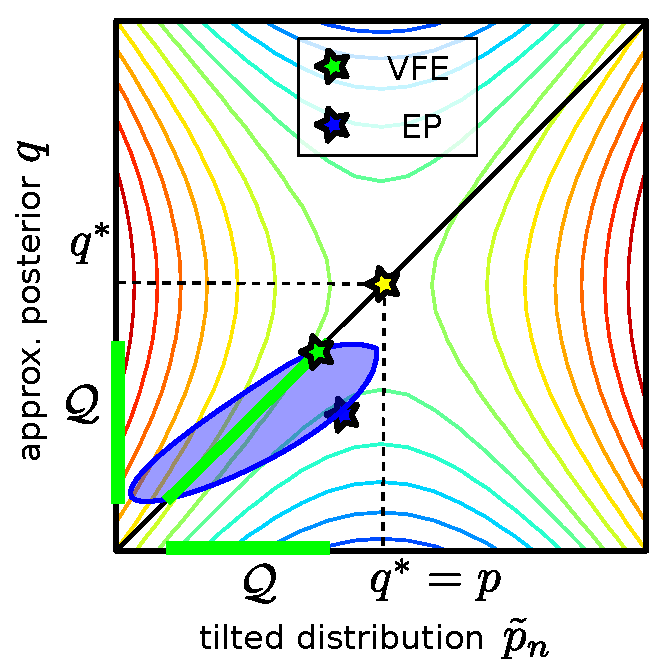
\includegraphics[width=0.4\linewidth]{Chapter2/ep/energy.pdf}
\caption{EP versus VI as constrained energy optimisation problems, visualised by projecting the energy surface from the augmented space $\mathcal{P}^{N+1}$ to $\mathcal{P}^{2}$. Here the slash line across the space represents the subspace $\{ (q, \tilde{p}_n): q = \tilde{p}_n \}$, and the search space for VI (the green segment) is contained in the EP candidate set (the blue region). The stars indicate the optimal solutions returned by the exact (in yellow) and the approximate inference algorithms (green/blue). See main text for details.}
\label{fig:chap2_ep_vi_comparison}
\end{figure}

\subsubsection{Criticisms for EP's iterative update}
%
The above fixed point iteration update has no convergence guarantee, which is one of the drawbacks of EP. The reason is that EP solves the dual problem of constrained Bethe free energy minimisation, and that dual problem turns out to be a minimax optimisation problem with constraints. Indeed, a double-loop algorithm \citep{heskes:ep2002} should be applied to (\ref{eq:ep_energy}) if convergence is required. However in practice such a double-loop method has been shown to be much slower than EP. Also disappointedly, even when the exact posterior is contained in $\mathcal{Q}$, EP is not guaranteed to return it. Similar problems exist for belief propagation when the graph contains many loops, or when the relaxed polytope is not \emph{tight} \citep{wainwright:graphical2008}.

%\hl{Another myth about EP is the choice of using fixed point update instead of gradient descent for the local parameters. Here it should be emphasised that the optimisation aims to find a \emph{saddle point} rather than a local minimum/maximum of the energy function. Since it is a minimisation problem for $\bm{\lambda}_q$ and maximisation problem for $\bm{\lambda}_{-n}$, is is also unclear to determine the optimisation problem for the local parameters $\bm{\lambda}_n$. Finally there exists no proof that the EP energy is upper or lower bounded, i.e. the existence of minimum/maximum is unclear as well. All the above situations make the analysis of gradient descent convergence very difficult.}


\subsubsection{From VFE to power EP}
\label{sec:vfe_to_pep}
We now extend the above approach to power EP \citep{minka:powerep2004} which is a new contribution, although fairly straightforward. This procedure includes one modification to the Bethe free energy. Assume for each factor $\tilde{f}_n$ a power value $\alpha_n \neq 0$ is associated, with $\bm{\alpha} = (\alpha_1, ..., \alpha_N)$ and $\sum_n \frac{1}{\alpha_n} \neq 1$. Then the Bethe free energy with moment matching constraints is modified to:
\begin{equation}
\mathcal{F}_{\bm{\alpha}}(q, \{ \tilde{p}_n \}) = \left( 1 - \sum_n \frac{1}{\alpha_n} \right) \mathrm{KL}[q||p_0] - \sum_{n=1}^N \frac{1}{\alpha_n} \mathbb{E}_{\tilde{p}_n} \left[ \log \frac{p_0(\mparam) \tilde{f}_n(\mparam)^{\alpha_n}}{\tilde{p}_n(\mparam)} \right].
\label{eq:alpha_bethe}
\end{equation}
%
Similar to the derivation of (\ref{eq:vi_constrained}), here we first added and subtracted $(\sum_n \frac{1}{\alpha_n})$ copies of $\mathrm{KL}[q||p_0]$, then decoupled $\tilde{p}_n$ from $q$, and relaxed the equality constraints to moment matching. Calculations following Section \ref{sec:ep_fixed_points} also reveal the change of the fixed point condition for $q$ to $(\sum_n \frac{1}{\alpha_n} - 1) \bm{\lambda}_q = \sum_n \frac{1}{\alpha_n} \bm{\lambda}_{-n}$. Define $q$ as an exponential family distribution with natural parameter $\bm{\lambda}_q$ as before, and $\bm{\lambda}_n = (\bm{\lambda}_q - \bm{\lambda}_{-n}) / \alpha_n$. We arrive at the power EP objective:
\begin{equation}
\left( \sum_n \frac{1}{\alpha_n} - 1 \right) \log Z_q - \sum_n \frac{1}{\alpha_n} \log \int p_0(\mparam) \tilde{f}_n(\mparam)^{\alpha_n} \exp \left[ (\bm{\lambda}_q - \alpha_n \bm{\lambda}_n)^T \bm{\Phi}(\mparam) \right] d \mparam.
\label{eq:pep_energy}
\end{equation}
The iterative process also enforces $\bm{\lambda}_q = \sum_n \bm{\lambda}_n$.  \cite{minka:divergence2005} showed that (\ref{eq:pep_energy}) becomes an upper-bound of $\log Z$ when $\alpha_n > 0$ and $\sum_n \frac{1}{\alpha_n} < 1$. On the other hand, taking $\alpha_n \rightarrow 0, \forall n$ recovers $\mathcal{F}_{\text{VFE}}$ but now the $q$ distribution is restricted to have an exponential family form.
% comparison
\section{A battle between VI and EP: which I should prefer?}

We have presented VI and EP as two main classes of approximate inference methods. Newcomers to this subject might be unsure about which algorithm they should use for their task. Inspired by the comparison table on the Infer.NET \citep{microsoft:infernet2014} user guide webpage,\footnote{\url{http://infernet.azurewebsites.net/docs/working\%20with\%20different\%20inference\%20algorithms.aspx}} here I put in Table \ref{tab:chap2_compare} a comparison between VI and EP, with discussions in the following. We note here again that VI is a special case of power EP by setting the power $\alpha=0$ (which is also referred to the variational message passing (VMP) algorithm \citep{winn:vmp2005, minka:divergence2005} that uses fixed-point iterative updates to optimise the variational lower-bound), and all the comparisons below are on VI versus power-EP with other $\alpha$ values. 

\begin{itemize}
\item Global versus local approximations. \\
%
As explained, VI constructs a \emph{global} approximation $q(\mparam) \approx p(\mparam|\data)$ while EP exploits the structure of the posterior distribution and proposes approximations to each of the factors instead (thus we call it \emph{local}). Interesting observations apply for VMP: like local approximation methods, it also propagates messages between factors and store approximations locally; like global approximation methods, however, any stationary point of the VMP algorithm is also a stationary point of the variational lower-bound, no matter which factor graph structure is in use. Conversely, EP returns different approximation results when executed on different factor graph representations of the target distribution. Due to this reason we still call VMP a \emph{global} approximation method, even when it also performs local computations.

\item Zero-forcing versus mass-covering behaviour. \\
VI exhibits zero-forcing behaviour exactly because it minimises the exclusive KL-divergence (see discussions in Section \ref{sec:chap2_kl_divergence}). For power EP the story is complicated: it can prefer mass-covering when having large $\alpha > 0$ values, but it can also be zero-forcing if, though not very often, negative $\alpha$ values are in use.

\item Convergence guarantee. \\
VI and VMP are guaranteed to converge, mainly because the variational lower-bound is upper-bounded. EP, like belief propagation on graphs, has no convergence guarantees in general, although practices suggest that it often converges to a local optimum.

\item Running time/speed. \\
VI with gradient descent often takes many iterations to converge, though each gradient step can be very cheap. EP, on the other hand, takes less iterations to run, but typically requires more time to compute the moment matching step. This is especially the case when there is no closed form solution for the moments, where an additional approximate inference procedure (e.g. MCMC) will be called as a sub-routine, which can be very expensive. VMP combines the advantages from both sides, often being the fastest method to find a local optimum.

\item Accuracy. \\
Assume both EP and VI use the same family of approximate distributions $\mathcal{Q}$. It is well known that variational free-energy approaches are biased and often severely so \citep{turner:two_problems2011}. Because of the zero-forcing behaviour, VI can be over-confident and miss important modes/correlation structure in the exact posterior. This often results in worse performance when calibrated uncertainty is required. EP is often more accurate when compared to VI, in some cases it can even be exact (e.g.~with a tree-structure graph containing simple factors like Gaussians). However EP can diverge on certain cases and in this case one might prefer VI to at least obtain a reasonable approximation.

\item Approximate posterior design. \\
VI with Monte Carlo methods allows the deployment of more complex approximate posterior distributions (e.g.~those parameterised by a neural network which will be introduced later). On the other hand, many applications of EP still use exponential family distributions (mainly Gaussians) until the development of Chapter \ref{chap:vrbound}.

\item Hyper-parameter optimisation and model selection. \\
One might want to optimise the hyper-parameters of the model, or perform model selection to choose the best model. Both cases require a reliable approximation to $\log p(\data)$. In this regard, VI provides a conservative (although possibly strongly biased) estimate of the marginal likelihood, which provides a safe option for approximate MLE. But EP's energy function can be hard to optimise: unless a fixed point is obtained, in theory the EP energy can be arbitrarily far from the exact marginal likelihood \citep{cunningham:gaussianEP2011}.\footnote{Although some empirical results suggest that it is possible to perform hyper-parameter optimisation at the same time as EP runs \citep{hernandez-lobato:gp2016}.} Even if EP converges, the corresponding energy function is not protected: it is neither an upper- nor a lower-bound to the model evidence.

\end{itemize}

Unfortunately I cannot provide a general case verdict for the two classes of algorithms, just like the folklore no-free lunch theorem \citep{wolpert:no_free_lunch1997} states ``there exists no machine learning algorithm that dominates the others in all cases''. To conclude the discussion, here comes two suggestions that have been validated by many results in the literature. Care should be taken for EP when the factor graph is densely connected and contains many loops. Also one should avoid using VI to approximate a non-smooth target density with a smooth $q$ distribution, because the zero-forcing behaviour of VI may push the approximate posterior towards undesirable solutions like delta mass. This happens, in binary classification for example, when the likelihood function is a Heaviside function or a very sharp sigmoid function. 

\begin{table}[t]
  \centering
  \caption{Comparing VI/VMP and power EP.}
  \renewcommand{\arraystretch}{1.2}
  \label{tab:chap2_compare}
  \begin{tabular}{ccc}
  	\toprule
      & VI/VMP & power EP ($\alpha \neq 0$)\\
    \hline
    %
    global or local? & \begin{tabular}{@{}c@{}} global \\ (same for VMP)  \end{tabular} &
    \begin{tabular}{@{}c@{}} local \\ (depends on the factor graph) \end{tabular}\\
    \hline
    behaviour & \begin{tabular}{@{}c@{}} zero-forcing \\  \end{tabular} &
    \begin{tabular}{@{}c@{}} zero-forcing/mass-covering \\ (depends on $\alpha$) \end{tabular}\\
    \hline
    \begin{tabular}{@{}c@{}} optimisation \\ procedure \end{tabular}  & \begin{tabular}{@{}c@{}} gradient descent (generic VI) \\ fixed-point iterative updates (VMP) \end{tabular} &
    \begin{tabular}{@{}c@{}} fixed-point iterative updates \\  \end{tabular}\\
    \hline
    convergence & \begin{tabular}{@{}c@{}} yes \\ (theoretical guarantee)  \end{tabular} &
    \begin{tabular}{@{}c@{}} yes (empirically) \\ (with log-concave potentials) \end{tabular}\\
    \hline
    accuracy & \begin{tabular}{@{}c@{}} often less accurate \\ (under-estimates uncertainty) \end{tabular} &
    \begin{tabular}{@{}c@{}} often more accurate \\ (depends on the factor graph) \end{tabular} \\
    \bottomrule
  \end{tabular}
  %\vspace{-0.1in}
\end{table}

\section{Applications: Bayesian deep learning}
Having discussed plenty of background material on divergences and approximate inference algorithms, in this section we turn to specify the probabilistic models that will be studied in the rest of the thesis. Historically, the Bayesian modelling community studied well-understood probabilistic models (conjugate models, generalised linear models, etc). Very recently the research theme of \emph{Bayesian deep learning} has received much increasing interest, where \emph{deep generative models} and \emph{Bayesian neural networks} are mainly studied. Advances in approximate inference sit at the core of Bayesian deep learning research: we will briefly sketch how VI can be used to perform inference and learning in both models. In later chapters we will also develop advanced approximate inference methods, and demonstrate improved performances on Bayesian deep learning tasks.

\subsection{Deep generative models}
\label{sec:chap2_dgm}
Generating realistic images, sound and text has always been one of the main themes in AI research. One approach towards this goal that is very popular now is building a \emph{deep generative model} to transform some random noise to desired outputs. Similar to the latent variable model we discussed in Section \ref{sec:chap2_amortisation}, the model starts from a latent variable $\z$ sampled from a prior distribution $p_0(\z)$, and then samples the observations $\x$ from a conditional distribution $p_{\mparam}(\x | \z)$ parameterised by $\mparam$.\footnote{It is possible to have a hierarchy of latent variable models, but here we will stick to the simplest case.} Unlike the linear case discussed before, here deep neural networks are applied to form the the likelihood $p_{\mparam}(\x | \z)$, usually by determining the parameters of the distribution by neural networks taking $\z$ as their input.\footnote{Another case where $p(\x | \z)$ is implicitly defined by neural network transforms will be discussed in the second part of the thesis.} 
%
As a concrete example, let us consider the following model:
\begin{equation*}
\z_n \sim \mathcal{N}(\z; \bm{0}, \bm{I}), \quad \x_n \sim \mathcal{N}(\x; \bm{\mu}_{\mparam}(\z_n), \text{diag}(\bm{\sigma}^2_{\mparam}(\z_n) ) ),
\end{equation*}
where $\bm{\mu}_{\mparam}$ and $\bm{\sigma}_{\mparam}$ are defined by deep neural network transforms of $\z$. With the observed dataset $\data = \{ \x_n \}_{n=1}^N$ in hand, we are interested in finding the most likely configuration of the neural network parameters $\mparam$ by maximum likelihood:
\begin{equation}
\max_{\mparam} \sum_{n=1}^N \log p_{\mparam}(\x_n),
\end{equation} 
which involves integrating out all the latent variables $\z_n$ out and which is thus analytically intractable. Traditionally, the expectation maximisation (EM) algorithm \citep{dempster:em1977} is used here to train the parameters $\mparam$. But here we deploy another approach which uses the variational lower-bound as a surrogate loss:
\begin{equation}
\max_{\mparam, \vparam} \sum_{n=1}^N \mathcal{L}_{\text{VI}}(\vparam, \mparam; \x_n), \quad \mathcal{L}_{\text{VI}}(\vparam, \mparam; \x) = \mathbb{E}_{q_{\vparam}(\z | \x)} \left[ \log \frac{p_{\mparam}(\x, \z)}{q_{\vparam}(\z|\x)} \right].
\end{equation}
The amortised variational inference algorithm is deployed (see Section \ref{sec:chap2_amortisation}). 

Here we introduce a neat trick called \emph{reparameterisation} \citep{kingma:vae2014, rezende:vae2014},\footnote{As we shall see this is \emph{not} a new trick, although \cite{kingma:vae2014} and \cite{rezende:vae2014} were the first to apply it in deep generative modelling context.} which, along with MC approximation, makes the variational lower-bound easy to handle. This trick comes from a very simple observation: given a distribution $p(\z)$, if sampling $\z \sim p(\z)$ is equivalent to first sampling a ``noise'' variable $\bm{\epsilon} \sim p(\bm{\epsilon})$ and then computing a mapping $\z = \bm{f}(\bm{\epsilon})$, then the expectation of some function $F(\z)$ under distribution $p(\z)$ can be rewritten as
$$ \mathbb{E}_{p(\z)} [ F(\z) ] = \mathbb{E}_{p(\bm{\epsilon})} [ F(\bm{f}(\bm{\epsilon})) ]. $$
%
This convenient computation is also called the \emph{law of the unconscious statistician} (LOTUS). To see how this trick works in the context of deep generative models, we consider a simple approximate posterior distribution, namely the factorised Gaussian:
\begin{equation*}
q_{\vparam}(\z | \x) = \mathcal{N}(\z; \bm{\mu}_{\vparam}(\x), \text{diag}(\bm{\sigma}^2_{\vparam}(\x) ) ).
\end{equation*}
Again $\bm{\mu}_{\vparam}$ and $\bm{\sigma}_{\vparam}$ are mappings parameterised by deep neural networks with parameter $\vparam$. One can easily notice that drawing samples from this Gaussian is done by the following procedure
\begin{equation}
\z \sim q_{\vparam}(\z|\x) \Leftrightarrow \bm{\epsilon} \sim q(\bm{\epsilon}) = \mathcal{N}(\bm{\epsilon}; \bm{0}, \bm{I}), \z = \bm{\mu}_{\vparam}(\x) + \bm{\sigma}_{\vparam}(\x) \odot \bm{\epsilon},
\label{eq:chap2_gaussian_reparam}
\end{equation}
where $\odot$ denotes element-wise product, and essentially (\ref{eq:chap2_gaussian_reparam}) performs a change-of-variable operation. Usually the two mappings $\bm{\mu}_{\vparam}(\cdot)$ and $\bm{\sigma}_{\vparam}(\cdot)$ are represented by (deep) neural networks (with $\vparam$ the network weight matrices), and in this context the $q$ distribution is also called the \emph{recognition model} or the \emph{inference network}. Following the LOTUS rule, the variational lower-bound can be rewritten as
\begin{equation}
\mathcal{L}_{\text{VI}}(\vparam, \mparam; \x) = \mathbb{E}_{q(\bm{\epsilon})} \left[ \log \frac{p_{\mparam}(\x, \bm{\mu}_{\vparam}(\x) + \bm{\sigma}_{\vparam}(\x) \odot \bm{\epsilon})}{q_{\vparam}(\bm{\mu}_{\vparam}(\x) + \bm{\sigma}_{\vparam}(\x) \odot \bm{\epsilon}  |\x)} \right],
\end{equation}
and it can be further approximated using simple Monte Carlo (MC):
\begin{equation}
\mathcal{L}^{\text{MC}}_{\text{VI}}(\vparam, \mparam; \x) = \frac{1}{K} \sum_{k=1}^K  \log \frac{p_{\mparam}(\x, \bm{\mu}_{\vparam}(\x) + \bm{\sigma}_{\vparam}(\x) \odot \bm{\epsilon}_k)}{q_{\vparam}(\bm{\mu}_{\vparam}(\x) + \bm{\sigma}_{\vparam}(\x) \odot \bm{\epsilon}_k  |\x)}, \quad \bm{\epsilon}_k \sim q(\bm{\epsilon}).
\label{eq:chap2_vae_objective_mc}
\end{equation}
%
In practice the MC estimate is computed with very few samples, and in the case of drawing only one sample ($K=1$), the resulting algorithm is very similar to training a standard auto-encoder with a noise-injected encoding operation, thus the name \emph{variational auto-encoder} \citep{kingma:vae2014, rezende:vae2014}. Its graphical model is also visualised in Figure \ref{fig:vae_figure}.

\begin{figure}[t]
\begin{center}
\begin{tikzpicture}[scale=1, transform shape]
\node[obs] (x1) {$\x$};
\node[latent, above=of x1] (z1) {$\z$};
\node[const, left=of z1] (phi1) {$\vparam$};
\node[const, right=of z1] (theta1) {$\mparam$};
\edge [dashed] {phi1} {z1};
\edge {theta1} {z1};
\edge {theta1} {x1};
\draw (x1) edge[out=135,in=225,->,dashed] (z1);
%\draw (z1) edge[out=315,in=45,->] (x1);
\edge {z1} {x1};
\plate [xscale=1.5] {} {(x1)(z1)} {$N$} ;
\end{tikzpicture}
\end{center}
\caption{
The graphical model of VAE, showing the generative model and the inference network. Dash arrows imply dependencies in the $q$ distribution. Reproduced from \cite{kingma:vae2014}.
}
\label{fig:vae_figure}
\end{figure}

%\vspace{1em}
%\begin{tcolorbox}
%\textbf{Remark} (Does the wake-sleep algorithm perform amortised inference?)\textbf{.}
%Deep learning community also refers the $q(\z | \x)$ distribution as \emph{recognition model/network} or \emph{inference network}. The name ``recognition model" is at least dated back to the development of Helmholtz machine \citep{dayan:helmholtz1995} which is trained using the wake-sleep algorithm \citep{hinton:ws1995}. Similar notions have also been adopted in \citep{morris:recognition2001} in the context of directed graphical models. Interestingly, the wake-sleep method uses exactly the MC-VI objective (\ref{eq:chap2_vae_objective_mc}) to learn the generative model, but optimises the ``recognition weights'' $\vparam$ by minimising $\mathbb{E}_{p_{\mparam}(\x)}[\mathrm{KL}[p_{\mparam}(\z | \x) || q_{\vparam}(\z | \x)]]$. Hence I do \emph{not} reckon the wake-sleep algorithm as performing amortised inference: the $q$ distribution is trained using samples $\x \sim p_{\mparam}(\x)$ rather than those from the training data, meaning that it is difficult to describe the approximation quality of $q$ when evaluated on $\x \sim \data$, and has no guarantee to return a good approximation to $p_{\mparam}(\z | \x)$. 
%%
%
%The above argument is still debatable: indeed $q$ is used to infer the latent variables $\z$ which is then used to train the $p$ model. The lower-bounding property of (\ref{eq:chap2_vae_objective_mc}) is true for \emph{any} $q_{\vparam}(\z | \x)$, so for those who does not care about the quality of the inference network $q$, this is indeed performing ``amortised inference'' in some sense. 
%%
%However as explained in Section \ref{sec:chap2_amortisation}, the goal of amortised inference is to \emph{find the global dependency in the approximate posterior distribution returned by a valid approximate inference method}.
%%
%Hence by examining this requirement, one can easily see that the wake-sleep algorithm does \emph{not} belong to such class of algorithms.
%%
%
%On the other hand, recent work on improving the wake-sleep algorithm \citep{bornschein:rws2015} proposed an adjusted sleep-step in order to incorporate the observations $\x \sim \data$. This makes the improved algorithm essentially equivalent to the importance weighted auto-encoder (IWAE) algorithm \citep{burda:iwae2016} which is indeed performing amortised inference in my opinion.
%
%\end{tcolorbox}


\subsection{Bayesian neural networks}
\label{sec:chap2_bnn}
Another exciting application of Bayesian inference is a class of methods called Bayesian neural networks (Bayesian NNs, BNNs), which maintains the uncertainty of the weight matrix assignments. Originated in the late 80s and early 90s in the last century \citep{peterson:mean_field1987, mackay:practical1992, neal:bnn1992, hinton:mdl1993, neal:thesis1995},\footnote{For a detailed history see \citep[Section 2.2.1]{gal:uncertainty2016}.} it has recently attracted a lot of attention again, mainly due to the advance of modern approximate inference techniques. In this thesis we will also study BNNs as a test case for the developed approximate algorithms, and here we provide a concise review of the related key concepts. 

We start by describing a normal deep neural network mapping $\y = \f_{\mparam}(\x)$ parameterised by a set of weights (and bias vectors which we omit here for simplicity) $\mparam = \{ \W^l \}_{l=1}^L$. Then given a training dataset $\data = \{ (\x_n, \y_n) \}_{n=1}^N$, one would first define a loss function $l(\y, \f_{\mparam}(\x))$ to measure the error between the supervision signal and the prediction, then train the neural network by minimising the empirical loss on the dataset
$$\min_{\mparam} \ \mathcal{F}(\mparam) = \sum_{n=1}^N l(\y_n, \f_{\mparam}(\x_n)).$$
Examples for such loss function include the mean squared error (or $\ell_2$ error) $l(\y, \f_{\mparam}(\x)) = || \y - \f_{\mparam}(\x) ||_2^2 $ for regression and cross entropy loss $l(\y, \f_{\mparam}(\x)) = -\y \log f_{\mparam}(\x) - (1 - \y) \log (1 - \f_{\mparam}(\x))$ for (binary) classification. To avoid overfitting, regularisers are often included in the optimisation objective, for example, adding an $\ell_2$ regulariser would return the following optimisation problem
\begin{equation}
\min_{\mparam} \ \mathcal{F}_{\text{MAP}}(\mparam) = \sum_{n=1}^N l(\y_n, \f_{\mparam}(\x_n) + \frac{\lambda}{2} || \mparam ||_2^2.
\label{eq:chap2_nn_map}
\end{equation}

Let us consider the above training objective again but from a probabilistic modelling perspective. In this case the network weight matrices $\mparam$ are treated as random variables, and a Gaussian prior $p_0(\mparam) = \N(\mparam; \bm{0}, \lambda^{-1} \mathbf{I})$ is attached.\footnote{Sometimes other prior distributions might be preferred, e.g.~spike-and-slab prior \citep{neal:thesis1995, louizos:bayesian_compression2017}.} For many loss functions (e.g.~$\ell_2$ loss), the likelihood function of $\mparam$ is then defined as\footnote{This definition requires $\int \exp( - l(\y, \f_{\mparam}(\x)) d\y$ to be finite, which is true for many loss functions but not always the case.} 
$$ p(\y | \x, \mparam) = \frac{1}{Z} \exp( - l(\y, \f_{\mparam}(\x)).$$
See \cite{lecun:energy2006} for an example justification. For most loss functions (e.g. mean square error and cross entropy) the normalising constant $Z$ does not depend on the weights $\mparam$. Given the training dataset $\data$ the joint distribution is 
$$ p(\data, \mparam) = p_0(\mparam) \prod_{n=1}^N p(\y_n | \x_n, \mparam),$$
thus one can easily show that the maximum a posteriori (MAP) training $\max_{\mparam} \log p(\data, \mparam) $ is exactly equivalent to the problem of (\ref{eq:chap2_nn_map}). 

After framing the deep neural network as a probabilistic model, a Bayesian approach would find the posterior of the network weights $p(\mparam| \data)$ and use the uncertainty information encoded in it for future predictions. Again the exact posterior is intractable, and approximate inference would fit an approximate posterior distribution $q_{\vparam}(\mparam)$ parameterised by the variational parameters $\vparam$ to the exact posterior, and then use it to compute the (approximate) predictive distribution.
%
As an example, here we consider a variational inference approach and write down the variational lower-bound accordingly \citep{hinton:mdl1993, barber:ensemble1998}
\begin{equation}
\mathcal{L}_{\text{VI}}(\vparam) = \sum_{n=1}^N \mathbb{E}_{q_{\vparam}} [ \log p(\y_n | \x_n, \mparam) ] - \KL[q_{\vparam}||p_0].
\label{eq:chap2_nn_vi}
\end{equation}
Solving problem (\ref{eq:chap2_nn_vi}) with a degenerate variational approximation $q_{\vparam}(\mparam) = \delta_{\mparam = \vparam}$ would result in a MAP solution (\ref{eq:chap2_nn_map}), which is less desirable in terms of capturing uncertainty. However $q_{\vparam}$ should also not be too complicated in terms of the entailed computational complexity, as now $\mparam$ is typically a very long vector of thousands, or even millions of dimensions. Popular choices of such ``efficient'' variational approximations include the mean-field Gaussian approximation
$$q_{\vparam}(\mparam) = \prod_{l=1}^L \prod_{i, j} \N(W_{ij}^l; \mu_{ij}^l, (\sigma_{ij}^l)^2 ), \quad \vparam = \{ \mu_{ij}^l, \sigma_{ij}^l \}_{i, j, l},$$
which doubles the number of parameters to be optimised, and which is thus less memory demanding than a correlated Gaussian approximation for example. Also now the KL term in (\ref{eq:chap2_nn_vi}) has an analytical solution
$$\KL[q_{\vparam}||p_0] = \sum_{i, j, l} \frac{1}{2} \left( \lambda (\mu_{ij}^l)^2 - 1 + \lambda (\sigma_{ij}^l)^2 - \log \lambda - 2 \log \sigma_{ij}^l \right) .$$ 
But even so the error term $\mathbb{E}_{q}[\log p(\y | \x, \mparam)]$ is intractable due to the highly non-linear NN mapping $\f_{\mparam}$. Fortunately this issue is mitigated by employing the Monte Carlo (MC) approximation again:
\begin{equation}
\mathcal{L}_{\text{VI}}^{\text{MC}}(\vparam) = \sum_{n=1}^N \frac{1}{K} \sum_{k=1}^K [ \log p(\y_n | \x_n, \mparam^k) ] - \KL[q_{\vparam}||p_0], \quad \mparam^k \sim q_{\vparam}(\mparam).
\end{equation}
Usually to reduce the number of forward passes (i.e. computing $\log p(\y | \x, \mparam)$) $K$ is often a small number, even as little as $K=1$. Also for large datasets stochastic optimisation techniques are also applied, meaning that for mini-batch training with a subset $\{ (\x_m, \y_m) \}_{m=1}^M \sim \data^M$, the objective is (e.g.~for $K=1$)
\begin{equation}
\mathcal{L}_{\text{VI}}^{\text{MC}}(\vparam) = \frac{N}{M} \sum_{m = 1}^M \log p(\y_m | \x_m, \mparam) - \KL[q_{\vparam}||p_0], \quad \mparam \sim q_{\vparam}(\mparam).
\label{eq:chap2_nn_mc_svi}
\end{equation}
If the KL divergence is intractable it can also be approximated by Monte Carlo, i.e. 
$$\KL[q_{\vparam}||p_0] \approx \log q_{\vparam}(\mparam) - \log p_0(\mparam), ~ \mparam \sim q_{\vparam}.$$
The reparameterisation trick discussed earlier is often applied to allow gradient back-propagation, and in the case of mean-field Gaussian approximations the weight matrices are sampled as $W_{ij}^l = \mu_{ij}^l + \sigma_{ij}^l \epsilon, ~ \epsilon \sim \N(\epsilon; 0, 1)$, and the log-likelihood terms in (\ref{eq:chap2_nn_mc_svi}) is then computed by $\log p(\y_m | \x_m, \bm{\mu} + \bm{\sigma} \odot \bm{\epsilon}) $.


\vspace{1em}
\begin{tcolorbox}
\textbf{Remark} (Other approximate inference methods for BNNs)\textbf{.}
Although we presented BNNs using VI, I shall point out that other approximate inference methods do apply.
Milestone papers of approximate inference techniques developed for BNNs include: Laplace approximation \citep{mackay:practical1992}, minimum description length \citep{hinton:mdl1993} (which is equivalent to VI), hybrid/Hamiltonian Monte Carlo \citep{neal:thesis1995}, and variational inference \citep{barber:ensemble1998, graves:practical2011, blundell:bnn2015, gal:dropout2016}. Recent applications of BNNs using non-VI Bayesian methods include stochastic gradient MCMC \citep[for example]{korattikara:dark2015, li:sgld_nn2016}, assumed density filtering/EP \citep{hernandez-lobato:pbp2015} and those that will be presented in the later Chapters.
\end{tcolorbox}


\section{Summary and outlook}

In this chapter we have established the idea of divergence minimisation, and reviewed two classes of commonly used approximate inference techniques: variational inference (VI) and expectation propagation (EP). These two methods are closely related to each other but also have notable differences, both algorithmically and in terms of the solutions they return. In the rest of the first part (chapters \ref{chap:factor_tying} and \ref{chap:vrbound}), we will study in depth these similarities and differences, and as a motivation for the detailed analysis we provide a brief discussion as follows.

First, compared to VI, EP brings more serious computational burden, in that its memory cost scales linearly with the number of factors in the graph representing the target density. Scalable approximations to EP are then discussed in Chapter \ref{chap:factor_tying}, in which we demonstrate the scalability of our proposals to machine learning tasks in which EP is too expensive to handle.

Second, both methods can be motivated by divergence minimisation, in which VI minimises the exclusive KL divergence and EP minimises an inclusive KL divergence. The generalisation, i.e.~power EP, minimises alpha-divergences which have the two KL divergences as special cases. However, VI performs \emph{global} divergence minimisation, while EP minimises the selected divergence \emph{locally}. The resulting differences in local optima and optimisation behaviour are further investigated in Chapter \ref{chap:vrbound}.
\chapter{Stochastic Expectation Propagation}
\label{chap:factor_tying}

% **************************** Define Graphics Path **************************
\ifpdf
    \graphicspath{{Chapter3/Figs/Raster/}{Chapter3/Figs/PDF/}{Chapter3/Figs/}}
\else
    \graphicspath{{Chapter3/Figs/Vector/}{Chapter3/Figs/}}
\fi

Scalable approximate inference is key to the recent success of Bayesian deep learning \citep{hernandez-lobato:pbp2015, blundell:bnn2015, gal:dropout2016}. Here scalability entails that the algorithm has low enough time and space complexity figures to be deployed on real-world datasets. By leveraging stochastic optimisation techniques, variational inference \citep{jordan:vi1999,beal:vi2003, hoffman:svi2013} has been shown to be highly scalable even for modelling datasets comprising millions of documents \citep{broderick:stream2013}. On the other hand, we have discussed at length in the last chapter why EP-like algorithms can be superior, which is indeed confirmed by a large set of \emph{small} scale experiments \citep{kuss:gpep2005,barthelme:ep_likelihood2014,cunningham:gaussianEP2011}.
%
As a reminder: EP constructs a posterior approximation by iterating simple local computations that refine factors which approximate the posterior contribution from \emph{each} datapoint. 

At first sight, EP might therefore appear well suited to large-data problems: the locality of computation makes the algorithm simple to be extended to stochastic optimisation scenarios. Indeed EP is certainly suited for fast approximate inference, and folklore suggests that it usually converges even faster than VI in practice, due to the exploitation of fixed-point iterative search. 
%
Despite the huge gain in time complexities, EP has garnered much less attention in the regard of large-scale learning tasks. This is because, the elegance of local computation has been bought at the price of a prohibitive memory overhead that grows with the number of data-points $N$, since each local approximating factor typically has the same complexity as the global approximation. In contrast, VI utilises global approximations that are refined directly, which prevents memory overheads from scaling with $N$. Thus VI is arguably better-suited for approximate Bayesian inference at large-scale, precisely because it is much more memory efficient (albeit if not utilising parallel computing).

Can we have the best of both worlds? That is, accurate global approximations that are derived from truly local computation. In this chapter we propose \emph{stochastic expectation propagation} (SEP) to address this question, which are developed based upon the standard EP algorithm. Importantly, SEP only maintains a global approximation (like VI), thus reducing the memory footprint by a factor of $N$ when compared to EP. However SEP updates the global approximation in a local way (like EP), with (damped) stochastic estimates on data sub-samples in an analogous fashion to stochastic variational inference (SVI) \citep{hoffman:svi2013}. Indeed, the generalisation of the algorithm to the power-EP setting directly recovers SVI as a special case. 
%
We further extend the method to control the granularity of the approximation, and to treat models with latent variables without compromising on accuracy or entailing unnecessary memory demands. Finally, we demonstrate the scalability and accuracy of the method on a number of real world and synthetic datasets, also spanning a number of canonical machine learning tasks.


%
To the best of my knowledge, the development of SEP back in 2015 was the first successful attempt\footnote{except for those using parallel computing where the memory constraint is not in consideration.} to scale-up EP-like algorithms to large-scale data and stochastic optimisation settings, which also inspired many innovations in Chapter \ref{chap:vrbound}, the black-box alpha algorithm \citep{hernandez-lobato:bbalpha2016}, and other applications.



%\section{Stochastic expectation propagation}
\label{sec:sep_all}

\vspace{1em}
\begin{tcolorbox}
\textbf{Remark} (Previous attempts to scale-up EP) \textbf{.}
As EP appears to be the method of choice for some applications, researchers have attempted to push it to scale. A first approach is to swallow the large computational burden and simply use large data-structures to store the approximating factors (e.g.~TrueSkill \citep{herbrich:trueskill2006}). This approach can only be pushed so far. A second approach is to use the \emph{assumed density filtering} (ADF) algorithm as a simple variant, which only requires a global approximation to be stored \citep{maybeck:adf1982}. ADF, however, provides poorly calibrated uncertainty estimates \citep{minka:ep2001} which was one of the main motivating reasons for developing EP in the first place. 
A third idea, complementary to the one described here, is to use approximating factors that have simpler structure (e.g.~low rank, \citep{qi+minka:sparseGP2010}). This reduces memory consumption (e.g.~for Gaussian factors from $\mathcal{O}(ND^2)$ to $\mathcal{O}(ND)$), but does not stop the scaling with $N$. A fourth idea uses EP to carve up the dataset \citep{gelman:dep2014,xu:sms2014} using approximating factors for collections of data-points. This results in coarse-grained, rather than local, updates and other methods must be used to compute them. (Indeed, the spirit of \cite{gelman:dep2014,xu:sms2014} is to extend sampling methods to large-datasets by exploiting EP's ability to split up inference problems into smaller parts, not EP itself.) 
\end{tcolorbox}

\section{Memory efficient factor tying}

\subsection{A quick comparison between EP and ADF}
%short review on EP
We begin by briefly setting-up the EP and assumed density filtering (ADF) algorithms for posterior approximation, and the readers are referred to Section \ref{sec:chap2_ep_algorithm} for a more detailed review. Recall that EP constructs the approximation $q(\mparam)$ to the exact posterior as the following:\footnote{Here we consider tractable prior distributions, e.g.~Gaussians, otherwise further approximation can be applied and the presented results carry in that case. } 
\begin{equation}
p(\mparam | \data) \approx q(\mparam), \quad p(\mparam | \data) \propto p_0(\mparam) \prod_{n=1}^{N} p(\bm{x}_n | \mparam), \quad q(\mparam) \propto p_0(\mparam) \prod_{n=1}^{N} f_n(\mparam).
\end{equation}
%
The goal of EP is to refine the approximate factors so that they capture the contribution of each of the likelihood terms to the posterior i.e.~$f_n(\mparam) \approx p(\bm{x}_n | \mparam)$. In this spirit, one approach would be to find each approximating factor $f_n(\mparam)$ by minimising the Kullback Leibler (KL) divergence between the posterior and the distribution formed by replacing one of the likelihoods by its corresponding approximating factor,  $\mathrm{KL}[p(\mparam|\data) || p(\mparam|\data) f_n(\mparam)/ p(\bm{x}_n | \mparam)]$. Unfortunately, such an update is still intractable as it involves computing the full posterior. Instead, EP approximates this procedure by replacing the exact leave-one-out posterior $p_{-n}(\mparam) \propto p(\mparam|\data) / p(\bm{x}_n | \mparam)$ on both sides of the KL by the approximate leave-one-out posterior (also called the \emph{cavity} distribution) $q_{-n}(\mparam) \propto q(\mparam)/f_n(\mparam)$. Since this couples the updates for the approximating factors, the updates must now be iterated.

We summarise the update procedure for a single factor in Algorithm \ref{alg:ep}. Critically, the approximation step of EP involves local computations since one likelihood term is treated at a time. The assumption is that these local computations, although possibly requiring further approximation, are far simpler to handle compared to the full posterior $p(\mparam| \data)$. In practice, EP often performs well when the updates are parallelised \citep{microsoft:infernet2014}. Moreover, by using approximating factors for groups of data-points, and then running additional approximate inference algorithms to perform the EP updates (which could include nested EP), EP carves up the data making it suitable for distributed approximate inference.

\begin{figure}[!t]
% UGLY USE OF \vspace & \hspace follows
\begin{minipage}[t]{0.32\linewidth}
\centering
\begin{algorithm}[H] 
\caption{EP} \small
\label{alg:ep} 
\begin{algorithmic}[1] 
	\STATE choose a factor $f_n$ to refine:
	\STATE compute cavity distribution \\$q_{-n}(\mparam) \propto q(\mparam) / f_n(\mparam)$ 
	\STATE compute tilted distribution \\$\tilde{p}_n(\mparam) \propto p(\bm{x}_n|\mparam) q_{-n}(\mparam)$
	\STATE moment matching: \\ \hspace{-5mm}$f_n(\mparam) \leftarrow \mathtt{proj}[\tilde{p}_n(\mparam)] / q_{-n}(\mparam) $
	\STATE inclusion:\\ $q(\mparam) \leftarrow q_{-n}(\mparam) f_n(\mparam)$\\\hspace{1mm}\\ \vspace{1.0mm} \hspace{1mm}\\
\end{algorithmic}
\end{algorithm}
\end{minipage}
%
\begin{minipage}[t]{0.32\linewidth}
\centering
\begin{algorithm}[H] 
\caption{ADF} \small
\label{alg:adf} 
\begin{algorithmic}[1] 
	\STATE choose a datapoint $\bm{x}_n\sim \data$:
	\STATE compute cavity distribution \\$q_{-n}(\mparam) = q(\mparam)$
	\STATE compute tilted distribution \\$\tilde{p}_n(\mparam) \propto p(\bm{x}_n|\mparam) q_{-n}(\mparam)$
	\STATE moment matching: \\ \hspace{-5mm}$f_n(\mparam) \leftarrow \mathtt{proj}[\tilde{p}_n(\mparam)] / q_{-n}(\mparam) $
	\STATE inclusion:\\ $q(\mparam) \leftarrow q_{-n}(\mparam) f_n(\mparam)$\\\hspace{1mm}\\ \vspace{1.0mm} \hspace{1mm}\\
\end{algorithmic}
\end{algorithm}
\end{minipage}
%\quad
\begin{minipage}[t]{0.32\linewidth}
\centering
\begin{algorithm}[H]
\caption{SEP} \small
\label{alg:sep} 
\begin{algorithmic}[1] 
%\STATE initialize $\{\tilde{f}_a\}$
	\STATE choose a datapoint $\bm{x}_n\sim \data$:
	\STATE compute cavity distribution \\ $q_{-1}(\mparam) \propto q(\mparam) / f(\mparam)$
	\STATE compute tilted distribution \\$\tilde{p}_n(\mparam) \propto p(\bm{x}_n|\mparam) q_{-1}(\mparam)$
	\STATE moment matching: \\\hspace{-5mm}$f_n(\mparam) \leftarrow \mathtt{proj}[\tilde{p}_n(\mparam)] / q_{-1}(\mparam) $
	\STATE inclusion:\\ $q(\mparam) \leftarrow q_{-1}(\mparam) f_n(\mparam)$
	\STATE \textit{implicit update}:\\ $f(\mparam) \leftarrow f(\mparam)^{1 - \frac{1}{N}} f_n(\mparam)^{\frac{1}{N}}$
\end{algorithmic}
\end{algorithm}
\end{minipage} 
%
%\caption{Comparing the Expectation Propagation (EP), Assumed Density Filtering (ADF), and Stochastic Expectation Propagation (SEP) update steps. Typically, the algorithms will be initialised using $q(\mparam) = p_0(\mparam)$ and, where appropriate, $f_n(\mparam)=1$ or $f(\mparam)=1$.}
\end{figure}

% ADF
There is, however, one wrinkle that complicates deployment of EP at scale. Computation of the cavity distribution requires removal of the current approximating factor, which means any implementation of EP must store them explicitly necessitating an $\mathcal{O}(N)$ memory footprint. One option is to simply ignore the removal step and replace the cavity distribution with the full approximation, resulting in the assumed density filtering (ADF) algorithm (Algorithm \ref{alg:adf}) \citep{maybeck:adf1982} that only maintains global approximation in memory. But as the moment matching step now over-counts the underlying approximating factor (consider the new form of the objective $\mathrm{KL}[q(\mparam) p(\bm{x}_n | \mparam) || q(\mparam)]$) the variance of the approximation shrinks to zero as multiple passes are made through the dataset. Early stopping, e.g.~after a single pass through the data, is therefore required to prevent overfitting, and generally speaking ADF does not return uncertainties that are well-calibrated to the posterior. 
%
In the next section we introduce a new algorithm that sidesteps EP's large memory demands whilst avoiding the pathological behaviour of ADF. 

\subsection{Stochastic expectation propagation}
%
% SEP
In this section we introduce a new algorithm, inspired by EP, called stochastic expectation propagation (SEP) that combines the benefits of local approximation (tractability of updates, distributability, and parallelisability) with global approximation (reduced memory demands).  The algorithm can be interpreted as a version of EP in which the approximating factors are tied, or alternatively as a corrected version of ADF that prevents overfitting. 
%
The key idea is that, at convergence, the approximating factors in EP can be interpreted as parameterising a global factor,  $f(\mparam)$, that captures the average effect of a likelihood on the posterior  $f(\mparam)^{N} = \prod_{n=1}^{N} f_n(\mparam) \approx \prod_{n=1}^{N} p(\bm{x}_n | \mparam)$. In this spirit, the new algorithm employs direct iterative refinement of a global approximation comprising the prior and $N$ copies of a single approximating factor, $f(\mparam)$, that is $q(\mparam) \propto f(\mparam)^N p_0(\mparam)$.

SEP uses updates that are analogous to EP's in order to refine $f(\mparam)$ in such a way that it captures the \emph{average} effect a likelihood function has on the posterior. First the cavity distribution is formed by removing one of the copies of the factor, $q_{-1}(\mparam) \propto q(\mparam)/f(\mparam)$. 
Second, the corresponding likelihood is included to produce the tilted distribution $\tilde{p}_n(\mparam) \propto q_{-1}(\mparam) p(\bm{x}_n | \mparam)$ and, third, SEP finds an intermediate factor approximation by moment matching, $f_n(\mparam) \leftarrow \mathtt{proj}[\tilde{p}_n(\mparam)] / q_{-1}(\mparam) $. Finally, having updated the factor, it is included into the approximating distribution. It is important here \emph{not} to make a full update since $f_n(\mparam)$ captures the effect of just a single likelihood function  $p(\bm{x}_n | \mparam)$. Instead, damping should be employed to make a partial update $f(\mparam) \leftarrow f(\mparam)^{1 - \epsilon} f_n(\mparam)^{\epsilon}$, and a natural choice uses $\epsilon = 1/N$ which can be interpreted as minimising  $\mathrm{KL}[\tilde{p}_n(\mparam) || p_{0}(\mparam)  f(\mparam)^N]$ in the moment update.

\begin{figure}
\centering
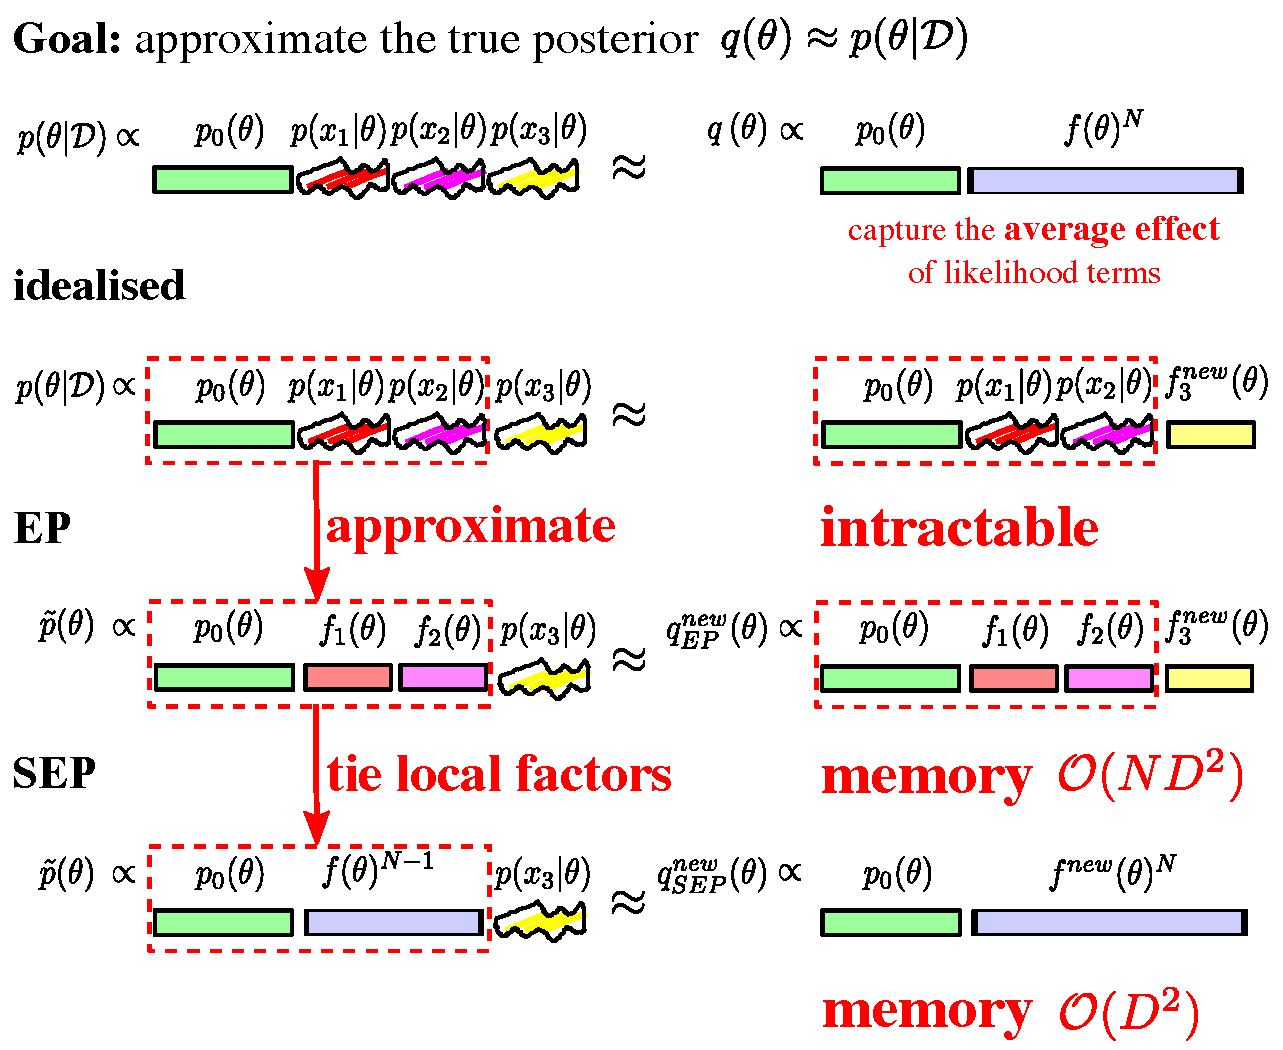
\includegraphics[width=1\linewidth]{Chapter3/sep/fig/algorithm_cartoon}
\caption{A cartoon visualisation for the comparison of three algorithms. Here the boxes represent the prior and the approximating factors, and both of them are assumed to be tractable. The wiggled objects are the complicated likelihood terms to be approximated. An idealised algorithm would approximate each of the likelihood terms given the others fixed as contextual information, which is intractable. EP replaces the ``contextual'' likelihood terms with the approximating factors to form a cavity distribution, making the moment matching step tractable. Finally, SEP ties all the approximating factors, and updates the tied factor by including one randomly sampled likelihood term at each iteration. The space complexity figures are calculated with the assumption of Gaussian approximation.}
\label{fig:chap3_sep_cartoon}
\end{figure}

SEP is summarised in Algorithm \ref{alg:sep}. Unlike ADF, the cavity is formed by dividing out $f(\mparam)$ which captures the average effect of the likelihood and prevents the posterior from collapsing. Like ADF, however, SEP only maintains the global approximation $q(\mparam)$ since $f(\mparam) \propto (q(\mparam) / p_0(\mparam))^{\frac{1}{N}}$ and $q_{-1}(\mparam) \propto q(\mparam)^{1 - \frac{1}{N}} p_0(\mparam)^{\frac{1}{N}}$. When Gaussian approximating factors are used, for example, SEP reduces the storage requirement of EP from  $\mathcal{O}(ND^2)$ to $\mathcal{O}(D^2)$ which is a substantial saving that enables models with many parameters to be applied to large datasets. We also provide a cartoon visualisation for motivating SEP in Figure \ref{fig:chap3_sep_cartoon}.


%




\section{Algorithmic extensions to SEP}
%
SEP has been motivated from a practical perspective by the limitations inherent in EP and ADF. In this section we extend SEP in four orthogonal directions and through these extensions relate SEP to SVI. Many of the algorithms described in this section are summarised in Figure \ref{fig:relationship-algorithms} and they are detailed in the following discussions.

\begin{figure}
\centering
\def\svgwidth{1\linewidth}
%\subfigure[\label{fig:relationship-algorithms}]{
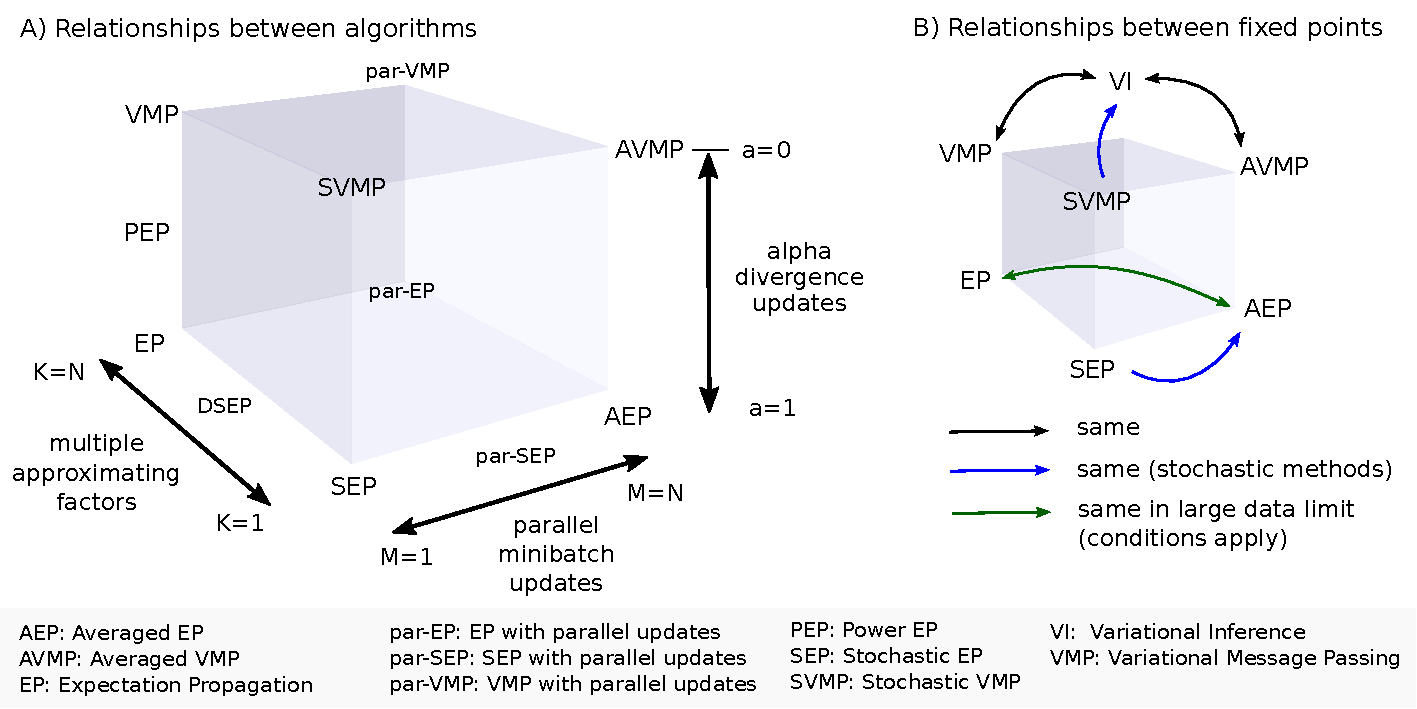
\includegraphics[height=6.5cm]{Chapter3/sep/fig/relationship-algorithms.pdf}%}
\caption{Relationships between algorithms. Note that care needs to be taken when interpreting Minka's alpha-divergence as $a \rightarrow 0$. See the main text for further discussions.}
\label{fig:relationship-algorithms}
\end{figure}

%
\subsection{Parallel SEP: relating the EP fixed points to SEP}
%

The SEP algorithm outlined above approximates one likelihood at a time which can be computationally slow. However, it is simple to parallelise the SEP updates by following the same recipe by which EP is parallelised. Consider a minibatch comprising $M$ datapoints (for a full parallel (batch) update use $M=N$). First we form the cavity distribution for each likelihood. Unlike EP these are all identical. Next, in parallel, compute $M$ intermediate factors $f_m(\mparam) \leftarrow \mathtt{proj}[\tilde{p}_m(\mparam)] / q_{-1}(\mparam)$. In EP these intermediate factors become the new likelihood approximations and the approximation is updated to $q(\mparam) = p_0(\mparam) \prod_{n \ne m} f_n(\mparam) \prod_{m} f_m(\mparam) $. In SEP, the same update is used for the approximating distribution, which becomes $q(\mparam) \leftarrow p_0(\mparam) f_{old}(\mparam)^{N-M} \prod_{m} f_m(\mparam) $ and, by implication, the approximating factor is $f_{new}(\mparam) = f_{old}(\mparam)^{1-M/N} \prod_{m=1}^M f_m(\mparam)^{1/N}$. One way of understanding parallel SEP is as a double loop algorithm. The \emph{inner loop} produces intermediate approximations  $q_m(\mparam) \leftarrow \arg\min_q \mathrm{KL}[\tilde{p}_m(\mparam) ||q(\mparam)]$; these are then combined in the \emph{outer loop}: $q(\mparam) \leftarrow \arg\min_q \sum_{m=1}^M \mathrm{KL}[q(\mparam) ||q_m(\mparam)] + (N-M) \mathrm{KL}[q(\mparam) || q_{old}(\mparam)]$.
%

For $M=1$ parallel SEP reduces to the original SEP algorithm. For $M=N$ parallel SEP is equivalent to the so-called Averaged EP (AEP) algorithm proposed in a concurrent work \citep{dehaene:aep2015,dehaene:aep2018} as a theoretical tool to study the convergence properties of normal EP. This work showed that when using Gaussian approximations, under fairly restrictive conditions,\footnote{e.g.~log likelihood functions that are smooth with bounding conditions up to the 4th-order derivative, although this is not a necessary condition.} AEP converges to the same fixed points as EP in the large data limit ($N \rightarrow \infty$).

There is another illuminating and arguably more direct connection between SEP and AEP. Since SEP's approximating factor $f(\mparam)$ converges to the geometric average of the intermediate factors $\bar{f}(\mparam) \propto [\prod_{n=1}^N f_n(\mparam)]^{\frac{1}{N}}$, SEP converges to the same fixed points as AEP, and therefore under certain conditions \citep{dehaene:aep2015,dehaene:aep2018}, to the same fixed points as EP. In practice decreasing learning rates, e.g. $\{\epsilon_t\}$ satisfying the Robbins and Monro criterion \citep{robbins:stochastic1951} $\sum_t \epsilon_t = \infty$, $\sum_t \epsilon_t^2 < \infty$, may be used to achieve convergence.
%
It is possible that there are more direct relationships between EP and SEP's dynamics, but that is still an open question.

\subsection{Stochastic power EP: relationships to variational methods}
The SEP algorithm generalises to the power-EP case in a straight-forward manner. Instead of removing one copy of the tied factors in Algorithm \ref{alg:sep}, when power $\alpha$ is in use we remove $\alpha$ fraction of the tied factors:
$$q_{-\alpha} \propto q(\mparam) / f(\mparam)^{\alpha}.$$
The moment matching step proceeds as in the power EP algorithm, precisely, 
$$f_n(\mparam)^{\alpha} \leftarrow \mathrm{proj}[ q_{-\alpha}(\mparam) p(\x_n | \mparam)^{\alpha} ] / q_{-\alpha}(\mparam) .$$
Similar to the power-EP case, the projection operator becomes I-projection when setting $\alpha \rightarrow 0$.

%
%NEED A PASS-THROUGH AGAIN
The relationship between variational inference and stochastic variational inference \citep{hoffman:svi2013} mirrors the relationship between EP and SEP. 
%
Can these relationships be made more formal? In the following we show that, if the moment projection step in EP is replaced by a natural parameter matching step (i.e.~I-projection) then the resulting algorithm is equivalent to the Variational Message Passing (VMP) algorithm \citep{winn:vmp2005, minka:divergence2005}. 

We first briefly sketch the VMP algorithm using the EP framework but replacing the moment matching step with natural parameter matching. We assume the approximate posterior $q(\mparam)$ is in some exponential family: 
\begin{equation}
q(\mparam) \propto \exp \left[ \langle \bm{\lambda}_q, \bm{\Phi}(\mparam) \rangle \right].
\end{equation}
At time $t$ we have the current estimate of the natural parameter $\bm{\lambda}_q^t$, which is defined as the sum of local variational parameters:
%
$\bm{\lambda}_q^t \buildrel\triangle\over = \bm{\lambda}_0 + \sum_{n=1}^N \bm{\lambda}_n^t$.\footnote{This notation implicitly assumes that the prior also belongs to the approximate distribution family $\mathcal{Q}$. In general we can propose another factor to approximate $p_0(\mparam)$, and our result still applies.}
%
Here $\bm{\lambda}_0$ represents the natural parameter of the prior distribution $p_0(\mparam)$. VMP iteratively computes the update of each local estimate $\bm{\lambda}_n^{t+1}$ in the following procedure. First VMP computes the expected sufficient statistics $\hat{\bm{s}}_n$ about datapoint $\bm{x}_n$ using $\bm{\lambda}_q^t$, e.g.~$\hat{\bm{s}}_n = E_{q}[t(z_n, x_n)]$ in the original SVI paper \citep{hoffman:svi2013}. Then VMP forms the gradient by differentiating the variational lower-bound but with $q_{-1}(\mparam)$ as the prior:
\begin{equation}
\nabla_{\bm{\lambda}_q^t} \mathcal{L}_{\text{VI}} \propto \bm{\lambda}_{-1}^t + \hat{\bm{s}}_n - \bm{\lambda}_q^t, \quad
\bm{\lambda}_{-1}^t := \bm{\lambda}_q^t - \bm{\lambda}_{n}^t.
\end{equation}
Next VMP zeros the gradient and recovers the current update $\bm{\lambda}_n^{t+1} = \hat{\bm{s}}_n$. The stochastic version of VMP, if extended in a way as SEP is developed from EP, defines the global variational parameters as $\bm{\lambda}_q^t \buildrel\triangle\over = \bm{\lambda}_0 + N \bm{\lambda}^t$. It computes the expected sufficient statistics $\hat{\bm{s}}_n$ in the same way as VMP but changes the cavity to $\bm{\lambda}_{-1}^t = \bm{\lambda}_q^t - \bm{\lambda}^t$ in the variational lower-bound maximisation steps. Readers can verify that this returns the current update $\bm{\lambda}^{t+1} = \hat{\bm{s}}_n$ using the important fact that the local update (for example $\hat{\bm{s}}_n = E_{q}[t(z_n, x_n)]$) \emph{only} depends on the global parameter $\bm{\lambda}_q^t$. Now since we tie all the local updates, the global parameter update $\bm{\lambda}_q^{t+1} = \bm{\lambda}_0 + N \bm{\lambda}^{t+1} = \bm{\lambda}_0 + N \hat{\bm{s}}_n$. In practice we perform a damped update, where a typical choice of step size is $\epsilon = 1/N$ like in SEP:
\begin{equation}
\bm{\lambda}_q^{t+1} \leftarrow (1 - \frac{1}{N}) \bm{\lambda}_q^t + \frac{1}{N}(\bm{\lambda}_0 + N \bm{\lambda}^{t+1}) = \bm{\lambda}_0 + (N-1) \bm{\lambda}^t + \hat{\bm{s}}_n.
\end{equation} 

On the other hand, \cite{mandt:smoothedSVI2014} summarises SVI as to compute the current update by zeroing the gradient
\begin{equation}
\nabla_{\bm{\lambda}_q} \mathcal{L}_{\text{VI}} \propto \bm{\lambda}_0 + N \hat{\bm{s}}_n - \bm{\lambda}_q,
\end{equation}
which returns $\bm{\lambda}_q^{t+1} = \bm{\lambda}_0 + N \hat{\bm{s}}_n$ as well. This implies that SVI, when using learning rate $\epsilon = 1/N$, is equivalent to SVMP. 
%
More generally, the procedure can be applied any member of the PEP family of algorithms, but care has to be taken when taking the limiting cases $\alpha \rightarrow 0$.
%
These results lend weight to the view that SEP is a natural stochastic generalisation of EP.

\subsection{Distributed SEP: controlling granularity of the approximation}
\label{sec:chap3_sep_dep}
EP uses a fine-grained approximation comprising a single factor for each likelihood. SEP, on the other hand, uses a coarse-grained approximation comprising a signal global factor to approximate the average effect of all likelihood terms. One might worry that SEP's approximation is too severe if the dataset contains sets of data-points that have very different likelihood contributions (consider classifying handwritten digits into odd and even classes, for example). 
It might be more sensible in such cases to partition the dataset into $J$ disjoint pieces $\{ \data_j = \{\bm{x}_n\}_{n=N_{j-1}}^{N_j} \}_{j=1}^{J}$ with $N = \sum_{j=1}^J N_j$ and use an approximating factor for each partition. If normal EP updates are performed on the subsets, i.e.~treating $p(\data_j |\mparam)$ as a single true factor to be approximated, we arrive at the distributed EP (DEP) algorithm \citep{gelman:dep2014, xu:sms2014}, summarised in Algorithm \ref{alg:dep} and detailed as the following.

%But such updates are challenging as multiple likelihood terms must be included during each update necessitating additional approximations (e.g.~MCMC). 
%A simpler alternative uses SEP/AEP \textbf{inside} each partition, which implies a posterior approximation of the form $q(\mparam) \propto p_0(\mparam) \prod_{j=1}^J f_{j}(\mparam)^{N_j}$ with $f_{j}(\mparam)^{N_j}$ approximating $p(\data_j|\mparam)$. The limiting cases of this algorithm, when $J=1$ and $J=N$, recover SEP and EP respectively. 

%We have shown in the main paper that a proper design of data partitioning improves SEP's approximation accuracy. This distributed algorithm is inspired by the Distributed EP (DEP) algorithm \cite{gelman:dep2014, xu:sms2014} presented in Algorithm \ref{alg:dep}. 

After data partitioning, the posterior distribution and likelihood functions are denoted as
\begin{align}
p(\mparam|\data) &\propto p_0(\mparam) \prod_{j=1}^J p(\data_j|\mparam), \\
p(\data_j|\mparam) &= \prod_{\bm{x}_n \in \data_j} p(\bm{x}_n | \mparam).
\end{align}
%
Next DEP assigns factors to each sub-dataset likelihood, i.e.~$q(\mparam) \propto p_0(\mparam) \prod_{j = 1}^J F_j(\mparam)$ with each $F_j(\mparam)$ approximating $p(\data_j|\mparam)$. The projection step is no longer analytically tractable in general since the tilted distribution with multiple data-points often lacks a simple form. Instead DEP handles moment matching by nesting additional approximations, e.g.~MCMC, which might be undesirable in terms of time complexity figures.

How does the factor tying idea apply in this case? A naive implementation would simply tie the sub-dataset level factors, but one should notice that $N_j$ might not be equal for different subsets. Instead we still construct datapoint level approximate factors similar to SEP, i.e.~$q(\mparam) \propto p(\mparam) f(\mparam)^N$, but construct the update in DEP fashion. In other words, $N_j$ factors are replaced by the likelihood terms in the $j$th subset in order to form the tilted distribution. Later these $N_j$ copies are updated by exactly the same moment matching step as in DEP. We name this algorithm stochastic EP \emph{on} data partitions and to distinguish from another algorithm presented later we abbreviate it as stochastic distributed EP (SDEP) (see Algorithm \ref{alg:sdep}). It is trivial to parallelise this method just as one would do for DEP, and we abbreviate the corresponding version as ADEP. 

%
To have a deterministic\footnote{in the sense that the moment matching step does not employ Monte Carlo.} counterpart of DEP, we consider SEP/AEP \emph{inside} each partition. This strategy might be preferred when one wish to carve up the data and carry out deterministic inference routines distributed across machines. We name this approach as Distributed SEP/AEP (DSEP/DAEP). Different to both DEP and SDEP, the approximate posterior for DSEP is defined as $q(\mparam) \propto p_0(\mparam) \prod_j f_j(\mparam)^{N_j}$, with $f_j(\mparam)^{N_j}$ approximating $p(\data_j|\mparam)$. The computations are almost the same as SEP/AEP except that the updates only modifies the copies of the corresponded subset. This method is also detailed in Algorithm \ref{alg:dsep}, and the differences between the two factor tying proposals are also visualised in Figure \ref{fig:chap3_dsep_compare}.

In summary, a flexible class of EP-like approximate inference algorithms can be derived, by carving up the dataset and designing the approximating factor structures and update procedures. Computational complexity figures are further presented in Section \ref{sec:chap3_complexity} to allow selections of algorithms confronting computation constraints.

\begin{figure}[t]
% UGLY USE OF \vspace & \hspace follows
\begin{minipage}[t]{0.32\linewidth}
\centering
\begin{algorithm}[H] 
\caption{DEP} \small
\label{alg:dep} 
\begin{algorithmic}[1]
	\STATE compute cavity distribution \\$q_{-j}(\mparam) \propto q(\mparam) / F_j(\mparam)$ \\  
	\STATE compute tilted distribution \\$\tilde{p}_j(\mparam) \propto p(\data_j|\mparam) q_{-j}(\mparam)$
	\STATE moment matching: \\ \hspace{-5mm}$F_j(\mparam) \leftarrow \mathtt{proj}[\tilde{p}_j(\mparam)] / q_{-j}(\mparam) $ \\
\hspace{1mm}\\ \vspace{12.2mm} \hspace{1mm}\\
\end{algorithmic}
\end{algorithm}
\end{minipage}
%\quad
\begin{minipage}[t]{0.32\linewidth}
\centering
\begin{algorithm}[H]
\caption{SDEP} \small
\label{alg:sdep} 
\begin{algorithmic}[1] 
%\STATE initialize $\{\tilde{f}_a\}$

	\STATE compute cavity distribution \\ $q_{-j}(\mparam) \propto q(\mparam) / f(\mparam)^{N_j}$
	\STATE compute tilted distribution \\$\tilde{p}_j(\mparam) \propto p(\data_j|\mparam) q_{-j}(\mparam)$
	\STATE moment matching: \\\hspace{-6mm}$F_j(\mparam) \leftarrow \mathtt{proj}[\tilde{p}_j(\mparam)] / q_{-j}(\mparam) $
	\STATE inclusion:\\\hspace{-6mm}$f(\mparam) \leftarrow f(\mparam)^{1 - N_j / N} F_j(\mparam)^{1/N}$ \\
\hspace{1mm}\\ \vspace{2.7mm} \hspace{1mm}\\
\end{algorithmic}
\end{algorithm}
\end{minipage} 
%
\begin{minipage}[t]{0.33\linewidth}
\centering
\begin{algorithm}[H] 
\caption{DSEP} \small
\label{alg:dsep} 
\begin{algorithmic}[1] 
	\STATE compute cavity distribution \\$q_{-1}(\mparam) = q(\mparam) / f_j(\mparam)$
	\STATE choose a datapoint \\ $\bm{x}_n \sim \data_j$
	\STATE compute tilted distribution \\$\tilde{p}_j^{(n)}(\mparam) \propto p(\bm{x}_n|\mparam) q_{-1}(\mparam)$
	\STATE moment matching: \\\hspace{-9mm}$f_j^{(n)}(\mparam) \leftarrow \mathtt{proj}[\tilde{p}_j^{(n)}(\mparam)] / q_{-1}(\mparam)$
	\STATE inclusion:\\\hspace{-8mm} $f_j(\mparam) \leftarrow f_j(\mparam)^{1 - 1/N_j} f_j^{(n)}(\mparam)^{1/N_j}$
\end{algorithmic}
\end{algorithm}
\end{minipage}
%
\end{figure}
%
\begin{figure}[ht]
\centering
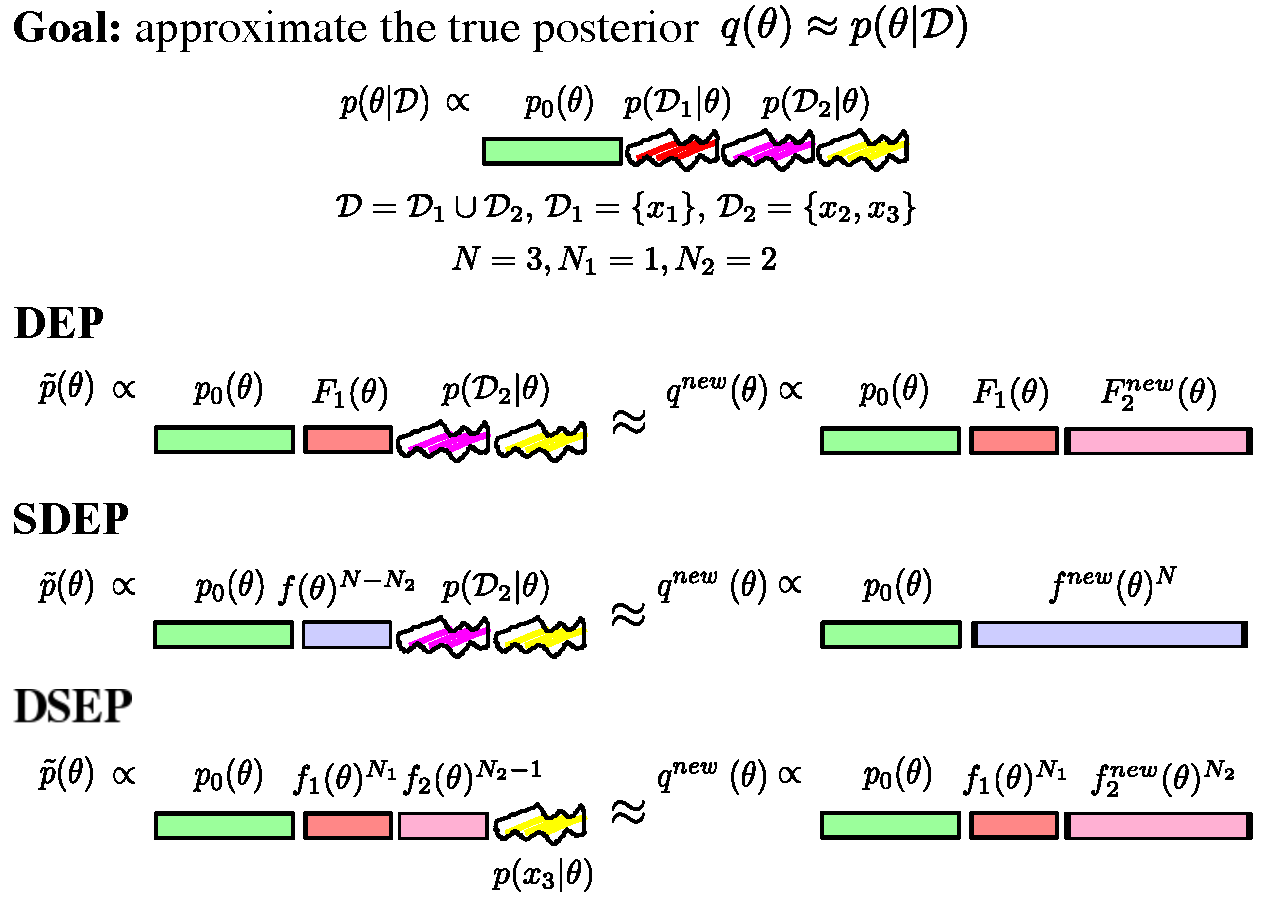
\includegraphics[width=1\linewidth]{Chapter3/sep/fig/dsep.pdf}
\caption{A cartoon visualisation on comparing DEP, SDEP and DSEP. One should notice that the definitions of $F_j(\mparam)$ in DEP is different from $f_j(\mparam)$ in DSEP. Here SDEP's moment matching step would typically require another approximate inference procedure, e.g.~simulating MCMC dynamics for a long time. On the other hand DSEP still use cheap updates computed on a single datum, which can be faster.}
\label{fig:chap3_dsep_compare}
\end{figure}

\subsection{SEP for latent variable models}

Many applications of EP involve latent variable models. Although this is not the main focus of the development, we show that SEP is applicable in this case and again it prevents the memory footprint from scaling with $N$. Critically as we shall see, the local factors $g_n(\z_n)$ do not need to be maintained in memory, although retaining them in memory might provide better initialisations that speeds up convergence potentially. This means that all of the advantages of SEP carry over to more complex models involving latent variables.

%
We consider a model containing latent variables $\z_n$ associated with each observation $\bm{x}_n$, which are drawn i.i.d.~from a prior $p_0(\z_n)$. SEP proposes approximations to the exact posterior over parameters and hidden variables 
\begin{equation}
p(\mparam, \{ \z_n\} | \data) \propto p_0(\mparam) \prod_n p_0(\z_n) p(\bm{x}_n | \z_n, \mparam)
\end{equation}
by tying the factors for the global parameter $\mparam$ but retaining the local factors for the hidden variables:
%
\begin{equation}
q(\mparam, \{ \z_n\}) \propto p_0(\mparam) f(\mparam)^N \prod_{n=1}^N g_n(\z_n) .
\end{equation}
In other words, SEP uses $f(\mparam) g_n(\z_n)$ to approximate $p(\bm{x}_n | \z_n, \mparam)p_0(\z_n)$.

Next we show a critical advantage of SEP for approximating latent variable posterior: the local factors $g_n(\z_n)$ do not need to be maintained in memory (again it might help to do so for better initialisation).
%
More formally, the cavity distribution is $q_{-n}(\mparam, \{ \z_n\}) \propto q(\mparam, \{ \z_n\})/(f(\mparam) g_n(\z_n)) $ and the tilted distribution is $$\tilde{p}_n(\mparam, \{ \z_n\}) \propto q_{-n}(\mparam, \{ \z_n\}) p(\bm{x}_n | \z_n, \mparam)p_0(\z_n).$$ This leads to a moment-update that minimises 
%
\begin{equation}
\mathrm{KL}[ p_0(\mparam) f(\mparam)^{N-1} p(\bm{x}_n | \z_n, \mparam)p_0(\z_n) \prod_{m\ne n} g_m(\z_m) || p_0(\mparam) f(\mparam)^{N-1} f'(\mparam) g_n(\z_n) \prod_{m\ne n} g_m(\z_m)] .\nonumber
\end{equation}
%
with respect to $f'(\mparam) g_n(\z_n)$. Importantly, the terms involving $\prod_{m\ne n} g_m(\z_m)$ are cancelled, meaning that these factors do not contribute to the local approximation step. For simple models the moments of $\z_n$ can be computed analytically given $q_{-1}(\mparam)$, thus $g_n(\z_n)$ is never stored in memory, resulting in a reduced memory footprint by a factor of $N$ again. 
%
It is also possible to have latent variables globally shared or shared in a data piece $\data_j$. But we can also extend SEP to these latent variables accordingly, which still provides computation gains in space complexity. In mathematical form, assume $\z_j$ a latent variable shared in $\data_j$. A prevalent example for this is the latent Dirichlet allocation (LDA) model \citep{blei:lda2003}, where $\data_j$ represents the $j^{\text{th}}$ document in the corpus and $\z_j$ represents the topic of the document. Then we construct $q(\z_j) \propto p_0(\z_j) g_k(\z_j)^{N_j}$ to approximate its posterior. This procedure still reduces memory by roughly a factor of $N/J$.
%

\vspace{1em}
\begin{tcolorbox}
\textbf{Remark} (amortised inference nested in SEP) \textbf{.}
In practice people may prefer maintaining the $g$ factors in memory, if the moment computation requires another optimisation inner-loop (which might be more expensive than the moment matching step itself). Examples of methods where this may be the case include latent Dirichlet allocation \citep{blei:lda2003} that has a hierarchy of latent variables, where VI methods also store variational $q$ distributions for some of the hidden variables. One potential recipe in this scenario is to apply amortised inference techniques, where in this case we can optimise the variational parameter $g_{\vparam}(\z_n | \x_n )$ for the factors attached to the latent variables. 
%Initial work with Vera Gangeskar Johne (for her Mphil thesis in Cambridge) on toy datasets suggested that this is a promising direction.
%
Another very closed related idea is to learn a model for the moments/messages passed in each SEP step with confidence estimates. A particular compelling feature of this approach is that one can control the use of the proposed message update by the model, and if rejected the algorithm can resort to the more expensive exact message computation using e.g.~MCMC. Interested readers are directed to \citep{heess:learning_messages2013, jitkrittum:kernel2015} for more details. 
\end{tcolorbox}

\section{Computational complexity}
\label{sec:chap3_complexity}
Besides the approximation accuracy, time and space complexities are also crucial for an efficient approximate inference algorithm to be widely-applicable, especially in systems that handle very large-scale datasets and also require fast computations. To provide a direct comparison between the methods discussed so far, we present the space and time complexity factors by considering Gaussian approximations with full covariance matrices. 

We assume an MCMC method is used for the DEP moment matching step, and assume it has time complexity $\mathcal{O}(H(n, D))$ if $n$ likelihood terms are involved and the random variable $\mparam$ is of dimension $D$, since it handles multiple likelihood functions at the same time for a single factor update. We also denote the time complexity factor of a normal EP moment matching step as $\mathcal{O}(h(D))$. Also since EP-like methods handle the natural parameters, for Gaussian approximations it requires $\mathcal{O}(D^3)$ time for matrix inversion and $\mathcal{O}(D^2)$ for matrix-vector multiplication in the inclusion step. By assumption EP's update step for a single factor can be done in a fast way, which means for a full pass through of the dataset $H(N, D) + D^3 + D^2 \geq N ( h(D) + D^3 + D^2)$. Furthermore in practice low-rank approximations can be applied to remove the $\mathcal{O}(D^3)$ factor if the random variable is very high dimensional, e.g.~see \cite{qi+minka:sparseGP2010} in EP literature. For the concern of memory usage, every factor in use occupies $\mathcal{O}(D^2)$ storage, although sparse approximations can significantly improve space complexity figures as well.

With all the above set-ups, we present the complexity figures in Table \ref{table:chap3_sep_complexity}, which apply to fully observed models, e.g.~Bayesian neural networks for classification tasks. Like the comparison between batch and stochastic learning methods, AEP-type methods produce more robust updates, and can be significantly faster than SEP-type methods if executed in parallel. However DEP/AEP algorithms require storing the factors in local worker machines, so in this regard SEP provides significant advantage in memory consumption in the price of slower convergence. 

\begin{table}[t]
\caption{Complexity figures for the EP algorithms discussed (with Gaussian approximations, full covariance matrices). The time complexity numbers are counted on a full pass of dataset, and the global approximations are updated after each moment computation. We assume the dataset is evenly split into $J$ disjoint subsets when applicable.}
\label{table:chap3_sep_complexity}
\begin{center}
\begin{tabular}{lll}
\multicolumn{1}{c}{\bf Algorithm}  &\multicolumn{1}{c}{\bf Time complexity} &\multicolumn{1}{c}{\bf Space complexity}
\\ \hline 
DEP (parallel)        	&$\mathcal{O}(D^3 + H(N/J, D) + D^2)$			&$\mathcal{O}(JD^2)$ \\
SDEP (sequel)        	&$\mathcal{O}(J(D^3 + H(N/J, D) + D^2))$			&$\mathcal{O}(D^2)$ \\
ADEP (parallel)        	&$\mathcal{O}(D^3 + H(N/J, D) + D^2)$			&$\mathcal{O}(JD^2)$ \\
DSEP (sequel)          &$\mathcal{O}(N(D^3 + h(D) + D^2))$ 		&$\mathcal{O}(D^2)$ \\
DAEP (parallel)         &$\mathcal{O}(J(D^3 + h(D) + D^2))$ 		&$\mathcal{O}(JD^2)$ \\
\hline
SEP 			         &$\mathcal{O}(N(D^3 + h(D) + D^2))$ 		&$\mathcal{O}(D^2)$ \\
AEP (parallel)		         &$\mathcal{O}(D^3 + h(D) + D^2)$ 		&$\mathcal{O}(ND^2)$ \\
ADF (multi.~pass) 		&$\mathcal{O}(N(h(D)))$ 		&$\mathcal{O}(D^2)$ \\
Normal EP         		&$\mathcal{O}(N(D^3 + h(D) + D^2))$ 		&$\mathcal{O}(ND^2)$ \\
\hline
Sampling 				&$\mathcal{O}(H(N, D))$			&$\mathcal{O}(D^2)$ \\
SVI 					&$\mathcal{O}(N(D^3 + \tilde{h}(D) + D^2))$	&$ \mathcal{O}(D^2)$ 
\end{tabular}
\end{center}
\end{table}

To conclude the discussion of computational efficiency we compare the complexity figures of SEP against those of SVI. Here we refer SVI to the general version which uses gradient descent, since the likelihood terms are very unlikely to be conjugate to the Gaussian approximation (thus the natural gradient descent algorithm \citep{hoffman:svi2013} does not apply). It is straightforward to see that both algorithms require the same amount of storage, which is $\mathcal{O}(D^2)$ in the Gaussian case. For the gradient descent update, as the gradient of the entropy term $\mathbb{H}[q]$ in the variational lower-bound requires computing the covariance matrix, this means the precision matrix as one of the natural parameters needs to be inverted. Therefore the cost for each gradient descent step in SVI is $\mathcal{O}(\tilde{h}(D) + D^3 + D^2)$, with $\mathcal{O}(D^3)$ the matrix inversion time, $\mathcal{O}(D^2)$ the update time for the precision matrix, and $\mathcal{O}(\tilde{h}(D))$ the computation time for the gradients of other terms in the variational lower-bound.
%
SVI might be more efficient in time complexity per iteration (i.e.~the runtime for processing one incoming observation, therefore $\tilde{h}(D) \leq h(D)$). However, as SEP uses fixed-point iterative updates, in practice SEP often converges in less passes of data than SVI thus is faster in total runtime, which is something that the above complexity analysis cannot take into account. For example \cite{hernandez-lobato:gp2016} showed that SEP, when applied to sparse GP classification, is significantly faster than SVI. SEP can be further accelerated using low-rank approximations when $D$ is large, which typically reduces the matrix inversion time to $\mathcal{O}(Dd^2)$ if we use rank-$d$ approximations.


\section{Experiments}

The purpose of the experiments was to evaluate SEP on a number of datasets (synthetic and real-world, small and large) and on a number of models (probit regression, mixture of Gaussians for clustering, and Bayesian neural networks).

%%%% SECOND EXAMPLE %%%%
\subsection{Bayesian probit regression}
\label{sec:chap3_exp_bayesian_probit}
%
The first experiments considered a simple Bayesian classification problem and investigated the stability and quality of SEP in relation to EP and ADF as well as the effect of using mini-batches and varying the granularity of the approximation. The model comprised a probit likelihood function $P(\bm{y}_n = 1|\theta) = \Phi(\bm{\theta}^T \bm{x}_n)$ and a Gaussian prior over the hyper-plane parameter  $p(\bm{\theta}) = \mathcal{N}(\bm{\theta}; \bm{0}, \gamma I)$.  
%
The synthetic data comprised $N=5,000$ datapoints $\{ (\bm{x}_n, \bm{y}_n) \}$, where $\bm{x}_n$ were $D=4$ dimensional and were either sampled from a single Gaussian distribution (Fig.~\ref{fig:sep_probit}) or from a mixture of Gaussians (MoGs) with 5 components (Fig.~\ref{fig:daep_probit}) to investigate the sensitivity of the methods to the homogeneity of the dataset. The labels were produced by sampling from the generative model. We followed \cite{xu:sms2014} to measure the performance by computing an approximation of $\mathrm{KL}[p(\bm{\theta}|\mathcal{D}) || q(\bm{\theta})]$, where $p(\bm{\theta}|\mathcal{D})$ was replaced by a Gaussian that had the same mean and covariance as samples drawn from the posterior using the No-U-Turn sampler (NUTS) \citep{hoffman:nuts2014}. This evaluation metric measures how close the approximated first and second moments are to those of the exact posterior, and emphasises well calibrated uncertainty estimations.

Results in Fig.~\ref{fig:sep_probit} indicate that EP is the best performing method and that ADF collapses towards a delta function. SEP converges to a solution which appears to be of similar quality to that obtained by EP for the dataset containing Gaussian inputs, but slightly worse when the MoGs was used. Variants of SEP that used larger mini-batches fluctuated less, but typically took longer times to converge (although for the small mini-batches shown this effect is not clear). The utility of finer grained approximations depended on the homogeneity of the data. For the second dataset containing MoGs inputs (shown in Fig.~\ref{fig:daep_probit}), finer grained approximations were found to be advantageous if the datapoints from each mixture component are assigned to the same approximating factor. Generally it was found that there is no advantage to retaining more approximating factors than there were clusters in the dataset.  

Although not a main purpose, we further test the performance of SEP with sampling methods to compute moments (i.e.~SDEP).\footnote{code adjusted from \texttt{ep-stan}: \url{https://github.com/gelman/ep-stan}} We re-use the settings of probit regression but change the probit unit to sigmoid function, making the moment projection analytically intractable. We randomly partition the dataset into $J = 20$ subsets $\{\mathcal{D}_j\}$, construct the approximate posterior with local factors over the subsets, and tie them in SEP/AEP as before. Note that we perform sequential computations for DEP and AEP although they are ideally suited for parallel computing. Again as presented in Figure \ref{fig:sep_logit}, SEP performs almost as well as EP, which further justifies SEP even with sampling methods. Also AEP is indistinguishable from DEP, but it reduces memory by a factor of $N/J$.

To see if the trends carry to real-world datasets, we tested SEP's performance on six small binary classification datasets from the UCI machine learning repository.\footnote{\url{https://archive.ics.uci.edu/ml/index.html}} We did not consider the effect of mini-batches or the granularity of the approximation, using $J=M=1$. We ran the tests with damping and stopped learning after convergence (by monitoring the updates of approximating factors). The classification results are summarised in Table \ref{tab:chap3_sep_probit_results}. ADF performs reasonably well on the mean classification error metric, presumably because it tends to learn a good approximation to the posterior mode. However, the posterior variance is poorly approximated and therefore ADF returns poor test log-likelihood scores. EP achieves significantly higher test log-likelihood than ADF indicating that a superior approximation to the posterior variance is attained. Crucially, SEP performs very similarly to EP, implying that SEP is an accurate alternative to EP even though it is refining a cheaper global posterior approximation.

\begin{figure}
\centering
\subfigure[\label{fig:sep_probit}]{
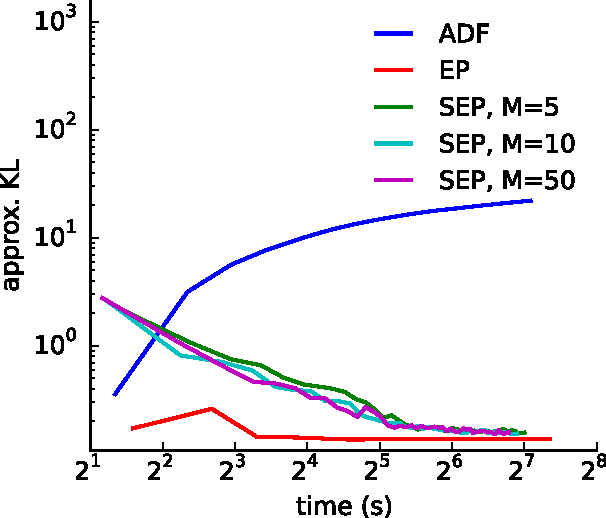
\includegraphics[width=0.30\linewidth]{Chapter3/sep/fig/sep_probit}}
%
\subfigure[\label{fig:daep_probit}]{
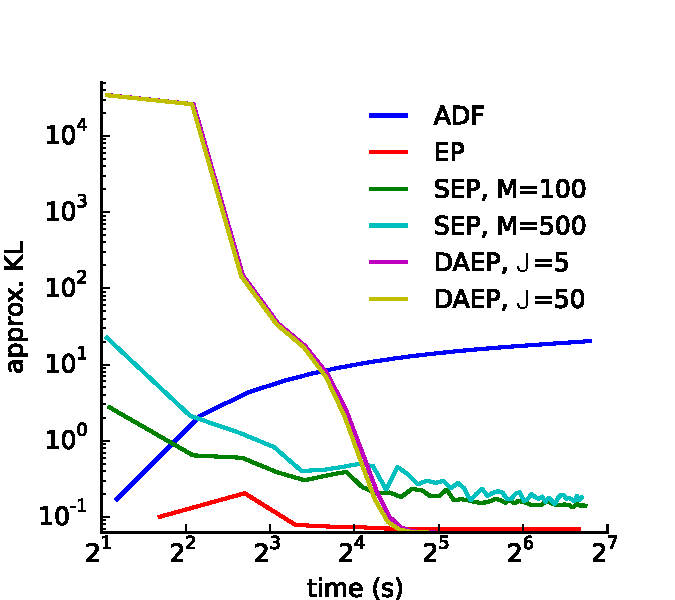
\includegraphics[width=0.35\linewidth]{Chapter3/sep/fig/daep.pdf}}
%
\subfigure[\label{fig:sep_logit}]{
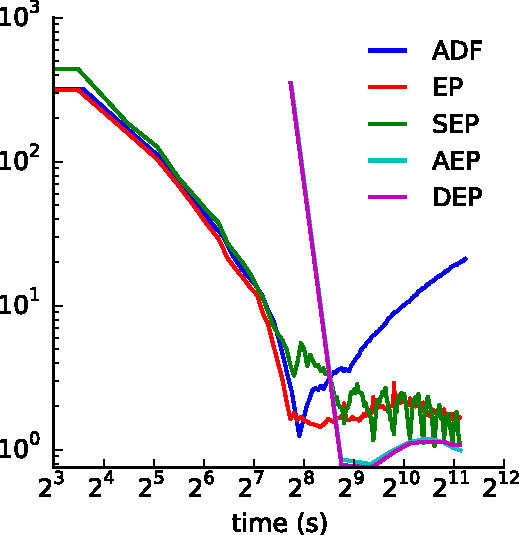
\includegraphics[width=0.26\linewidth]{Chapter3/sep/fig/sep_logit}}
\caption{Bayesian logistic regression experiments. Panels (a) and (b) show synthetic data experiments. Panel (c) shows the performance of EP-like methods on Bayesian logistic regression with the moment matching step computed by NUTS. $M$ denotes the mini-batch size for data sub-sampling (may be within a data piece for panel (c)). EP (in red curves) is the best performing method in terms of the approximate KL metric.  SEP works slightly worse but with its performance approaching to EP as the running time grows. ADF over-counts the number of observations and thus returns worst results as expected.}
\end{figure}

\begin{table} 
\small
\centering
 \caption{ Average test results all methods on probit regression (mean and standard error reported). All methods capture a good posterior mode, however EP outperforms ADF in terms of test log-likelihood on almost all the datasets, with SEP performing similarly to EP.}
  \label{tab:chap3_sep_probit_results} 
  \scalebox{0.9}{
\begin{tabular}{l@{\ica}r@{$\pm$}l@{\ica}r@{$\pm$}l@{\ica}r@{$\pm$}l | @{\ica}r@{$\pm$}l@{\ica}r@{$\pm$}
	l@{\ica}r@{$\pm$}l@{\ica}r@{$\pm$}}\hline 
{} & \multicolumn{6}{c}{mean error} & \multicolumn{6}{c}{test log-likelihood} \\
\bf{Dataset}&\multicolumn{2}{c}{\bf{ ADF }}&\multicolumn{2}{c}{\bf{ SEP }}&\multicolumn{2}{c}{\bf{ EP }} &\multicolumn{2}{c}{\bf{ ADF }}&\multicolumn{2}{c}{\bf{ SEP }}&\multicolumn{2}{c}{\bf{ EP }} \\ \hline 
%
Australian&0.328&0.0127&\bf{0.325}&\bf{0.0135}&0.330&0.0133
	&-0.634&0.010&\bf{-0.631}&\bf{0.009}&\bf{-0.631}&\bf{0.009}\\
%
Breast&0.037&0.0045&\bf{0.034}&\bf{0.0034}&\bf{0.034}&\bf{0.0039}
	&-0.100&0.015&-0.094&0.011&\bf{-0.093}&\bf{0.011}\\
%
% Crabs results after convergence
Crabs&0.056&0.0133&\bf{0.033}&\bf{0.0099}&0.036&0.0113
	&-0.242&0.012&-0.125&0.013&\bf{-0.110}&\bf{0.013}\\
% Crabs results for only 40 iterations (not converged)
%Crabs&0.062&0.0125&\bf{0.040}&\bf{0.0106}&0.048&0.0117
%	&-0.290&0.010&\bf{-0.177}&\bf{0.012}&-0.217&0.011\\
%
Ionos&\bf{0.126}&\bf{0.0166}&0.130&0.0147&0.131&0.0149
	&-0.373&0.047&-0.336&0.029&\bf{-0.324}&\bf{0.028}\\
%
Pima&0.242&0.0093&0.244&0.0098&\bf{0.241}&\bf{0.0093}
	&-0.516&0.013&-0.514&0.012&\bf{-0.513}&\bf{0.012}\\
%
Sonar&\bf{0.198}&\bf{0.0208}&\bf{0.198}&\bf{0.0217}&\bf{0.198}&\bf{0.0243}
	&-0.461&0.053&-0.418&0.021&\bf{-0.415}&\bf{0.021}\\
 \hline \end{tabular} }
 \end{table} 
 
\subsection{DSEP experiments and grouping tests}

The assumption we made in the main text to achieve SEP $\approx$ full EP is that the contributions of each likelihood term to the posterior are very similar. We show further results here on the approximation produced by different EP methods when we believe there exists heterogeneity in data.
%
We generated synthetic XOR classification data by sampling from 4 unit Gaussians with means $(3, 3)$, $(-3, -3)$, $(3, -3)$ and $(-3, 3)$, and labelling the clusters centred at the former two as negative examples (and positive for the others). The model $p(y_n|\bm{x}_n, \bm{\theta})$ is kernel probit regression using RBF kernel with width $l=1.0$, which is the same as the model presented in Section \ref{sec:chap3_exp_bayesian_probit} except that the features are changed to kernel representations. This makes the feature vectors high dimensional, and the local nature of kernels also makes them very different if the datapoints belong to different clusters. We generated $50 \times 4$ test data and $\{10 \times 4, 20 \times 4, 50 \times 4\}$ training data and ran SEP/DSEP/full EP to approximate the posterior distribution of $\bm{\theta}$. For DSEP we partitioned the dataset into 4 subsets according to the associated centroid. Each experiment was repeated 10 times to collect average test data log-likelihood and classification error.

Table \ref{tab:kernel} shows the quantitative numbers of performances and Figure \ref{fig:kernel_increase_n} visualises the contours of probability $p(y = 1|\bm{x}, \mathcal{D})$ with true posterior approximated by $q(\bm{\theta})$. Interestingly SEP is slightly better then the others on the classification error metric. But importantly EP achieves the best test log-likelihood numbers and in general DSEP produces very similar results (shown by both the table and the figure), meaning that even for small datasets running full EP might be unnecessary. Also the three methods become indistinguishable when the size of the dataset $N$ increases. We argue the main reason is that the posterior contributions are getting similar since more datapoints are observed in the circle of kernel width.

We further tested the robustness of all three methods to outliers. We reused the settings above and randomly flipped $10\%$ labels of training data. Qualitative results in Figure \ref{fig:kernel_flip} show that SEP is almost as robust as DSEP/EP in this example. We had tried different types of outliers and failed to find the cases where EP/DSEP significantly outperforms SEP. Future work should answer the questions that when SEP gives bad approximations and whether it fails in the same way as EP fails.


\begin{table} 
\small
\centering
 \caption{ Average test results of all methods on kernel probit regression.}
  \label{tab:kernel} 
  \scalebox{0.9}{
\begin{tabular}{l@{\ica}r@{$\pm$}l@{\ica}r@{$\pm$}l@{\ica}r@{$\pm$}l@{\ica}r@{$\pm$}l@{\ica}r@{$\pm$}
	l@{\ica}r@{$\pm$}l@{\ica}r@{$\pm$}}\hline 
{} & \multicolumn{6}{c}{mean error} & \multicolumn{6}{c}{test log-likelihood} \\
\bf{$N$}&\multicolumn{2}{c}{\bf{ SEP }}&\multicolumn{2}{c}{\bf{ DSEP }}&\multicolumn{2}{c}{\bf{ EP }} &\multicolumn{2}{c}{\bf{ SEP }}&\multicolumn{2}{c}{\bf{ DSEP }}&\multicolumn{2}{c}{\bf{ EP }} \\ \hline 
%
$10 \times 4$&\bf{0.032}&\bf{0.0058}&0.055&0.0127&\bf{0.032}&\bf{0.0097} 
	&-0.405&0.011&-0.380&0.010&\bf{-0.378}&\bf{0.009} \\
%
$20 \times 4$&\bf{0.007}&\bf{0.0014}&0.008&0.0024&0.012&0.0031 
	&-0.326&0.007&-0.320&0.006&\bf{-0.317}&\bf{0.003} \\
%
$50 \times 4$&\bf{0.003}&\bf{0.0010}&\bf{0.003}&\bf{0.0014}&0.006&0.0009 
	&-0.243&0.004&\bf{-0.233}&\bf{0.007}&-0.238&0.003 \\
%
 \hline \end{tabular} }
 \end{table} 

\begin{figure}
\centering
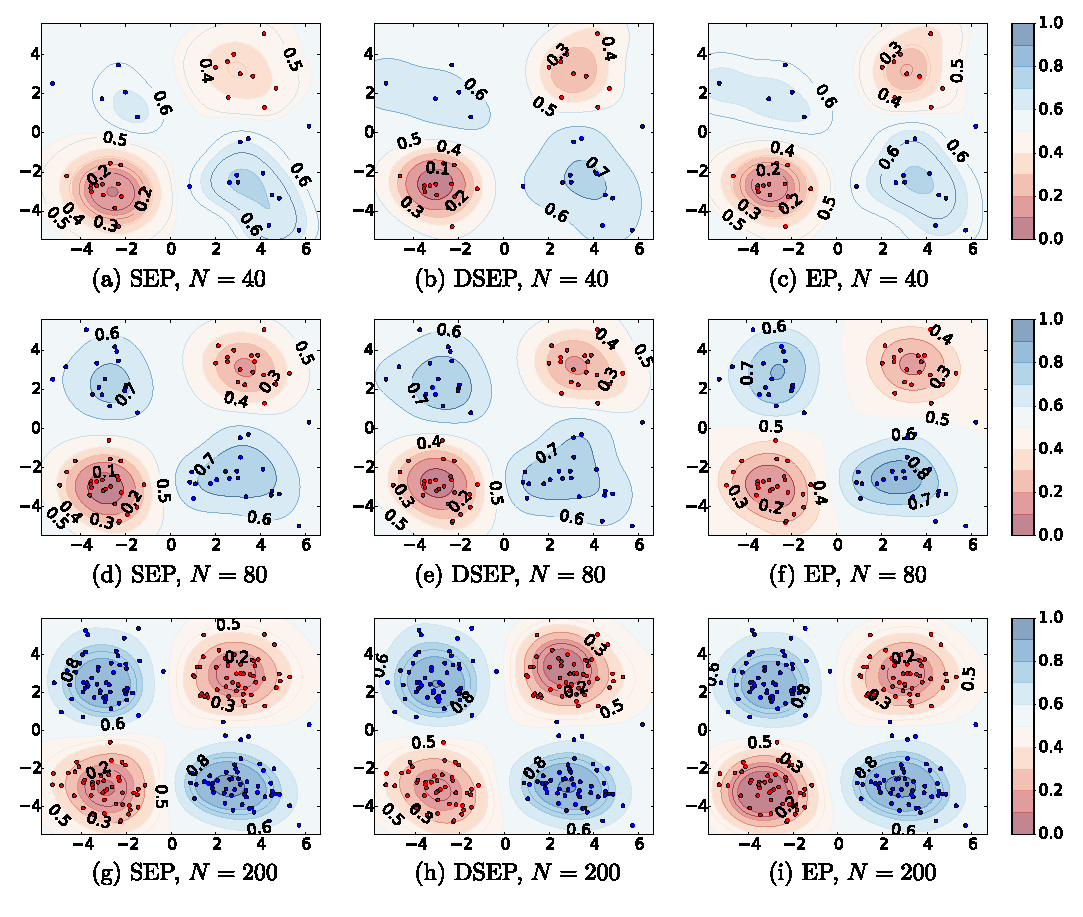
\includegraphics[width=1\linewidth]{Chapter3/sep/fig/increase_n_kernel}
\caption{Comparing predictions of kernel Probit regression trained by SEP/DSEP/EP, with increasing training data size $N$. Although not very significant, for $N=40$ the decision boundary obtained by the DSEP method is more similar to that of the full-EP method. This difference vanishes as $N$ increases. }
\label{fig:kernel_increase_n}
\end{figure}

\begin{figure}
\centering
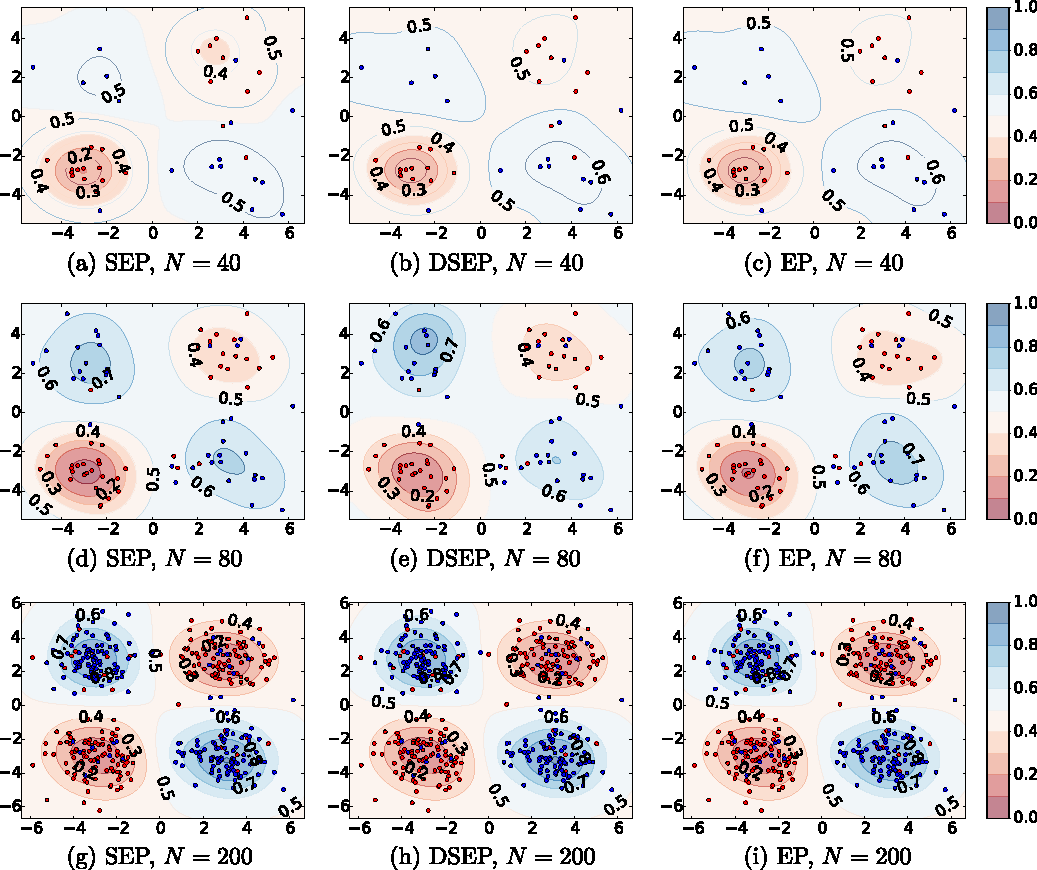
\includegraphics[width=1\linewidth]{Chapter3/sep/fig/flip_kernel}
\caption{Comparing predictions of kernel probit regression trained by SEP/DSEP/EP, with $10\%$ labels flipped. The same observations as to the results in \ref{fig:kernel_increase_n} apply.}
\label{fig:kernel_flip}
\end{figure}

To verify whether these conclusions about the granularity of the approximation hold in real datasets, we sampled $N=1,000$ datapoints for each of the digits in MNIST and performed odd-vs-even classification. Each digit class was assigned its own global approximating factor, $J=10$. We compare the log-likelihood of a test set using ADF, SEP ($J=1$), full EP and DSEP ($J=10$) in Figure \ref{fig:mnist}. EP and DSEP significantly outperform ADF. DSEP is slightly worse than full EP initially, however it reduces the memory to 0.001\% of full EP without losing substantial accuracy. SEP's accuracy was still increasing at the end of learning and was slightly better than ADF.

\begin{figure}
\centering
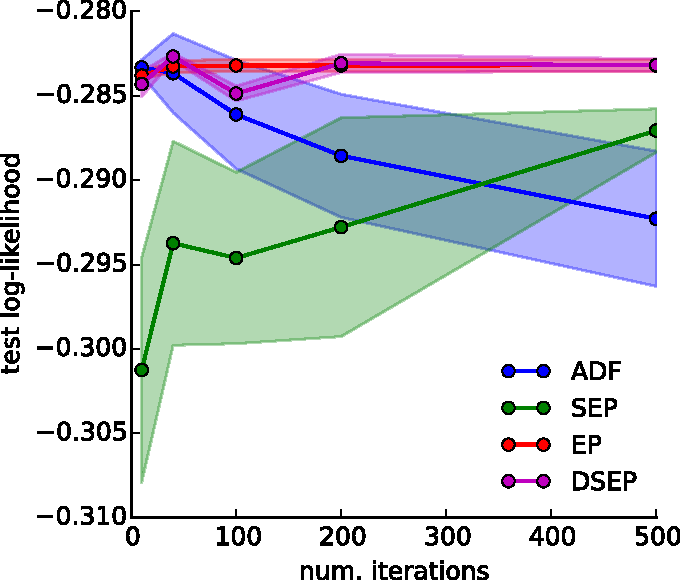
\includegraphics[width=0.4\linewidth]{Chapter3/sep/fig/mnist_error}
\caption{DSEP experimental result on MNIST (mean and standard error reported, see text for full details).}
\label{fig:mnist}
\end{figure} 
 
 %
%%%% FIRST EXAMPLE %%%%
\subsubsection{Mixture of Gaussians for clustering}
%
The small scale experiments on probit regression indicate that SEP performs well for fully-observed probabilistic models. Although it is not the main focus of the section, we sought to test the flexibility of the method by applying it to a latent variable model, specifically a mixture of Gaussians (MoGs). A synthetic MoGs dataset containing $N=200$ datapoints was constructed comprising 4 Gaussians. The means were sampled from a Gaussian distribution, $p(\bm{\mu}_j)= \mathcal{N}(\bm{\mu}; \bm{m}, \mathbf{I})$, the cluster identity variables $\bm{h}_n$ were sampled from a uniform categorical distribution, and each mixture component was isotropic $p(\bm{x}_n | \bm{h}_n) = \mathcal{N}(\bm{x}_n; \bm{\mu}_{\bm{h}_n}, 0.5^2 \mathbf{I})$. EP, ADF and SEP were performed to approximate the joint posterior over the cluster means $\{ \bm{\mu}_j\}$ and cluster identity variables $\{ \bm{h}_n \}$ (the other parameters were assumed known). 

Figure \ref{fig:gmm_visualised} visualises the approximate posteriors after 200 iterations. All methods return good estimates for the means, but ADF collapses towards a point estimate as expected. SEP, in contrast, captures the uncertainty and returns nearly identical approximations to EP. The accuracy of the methods is quantified in Fig.~\ref{fig:gmm_error} by comparing the approximate posteriors to those obtained from NUTS. In this case the approximate KL-divergence measure is analytically intractable, instead we used the averaged Frobenius-norm (F-norm) of the difference of the Gaussian parameters fitted by NUTS and EP methods. These measures confirm that SEP approximates EP well.

\begin{figure}
\centering
\subfigure[\label{fig:gmm_visualised}]{
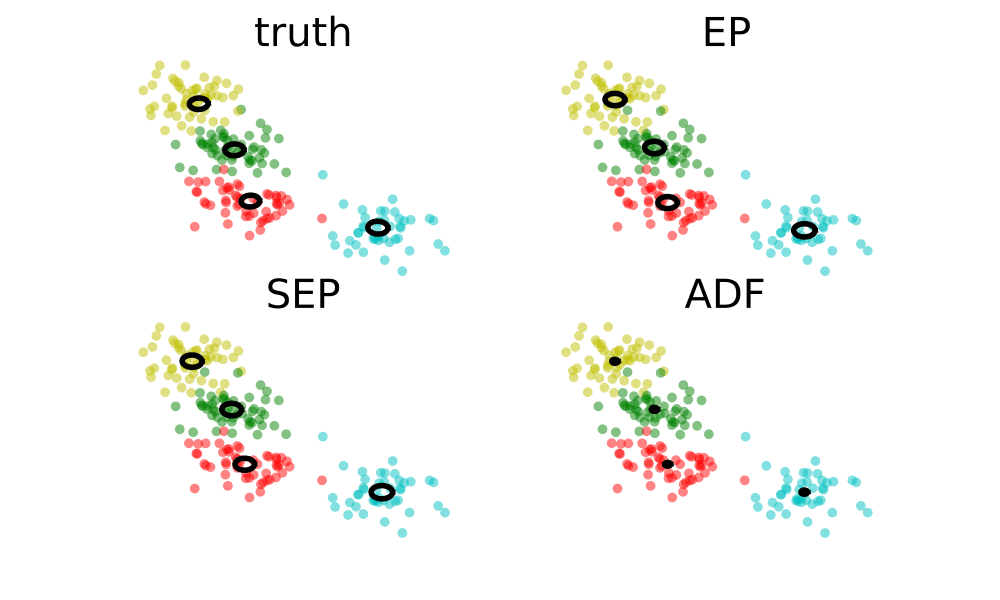
\includegraphics[width=0.5\linewidth]{Chapter3/sep/fig/gmm1.png}}
%
\hspace{0.1in}
%
\subfigure[\label{fig:gmm_error}]{
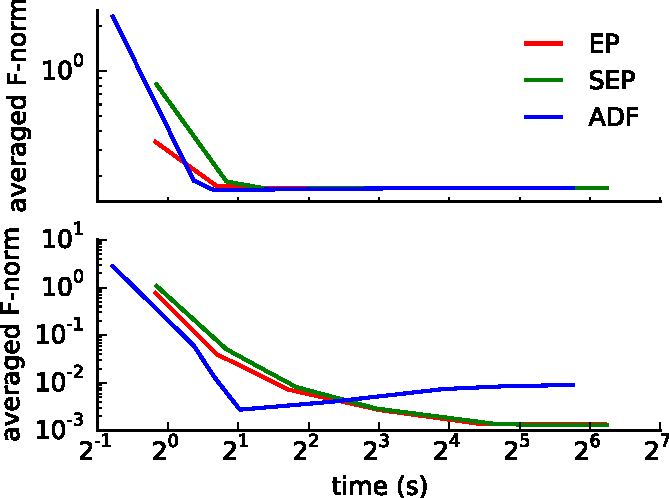
\includegraphics[width=0.42\linewidth]{Chapter3/sep/fig/gmm_error}}
\caption{Posterior approximation for the mean of the Gaussian components. (a) visualises posterior approximations over the cluster means (98\% confidence level). The coloured dots indicate the true label (top-left) or the inferred cluster assignments (the rest). In (b) we show the error (in F-norm) of the approximate Gaussians' means (top) and covariances (bottom). }
\end{figure}

\subsection{Probabilistic back-propagation for Bayesian neural nets}

The final set of tests consider more complicated models and large datasets. Specifically we evaluate the methods for probabilistic back-propagation (PBP) \citep{hernandez-lobato:pbp2015}, a
recent state-of-the-art method for scalable Bayesian learning in neural
network models.\footnote{See Appendix \ref{sec:appendix_pbp} for detailed update equations.} Previous implementations of PBP perform several iterations of ADF over the training
data. The moment-matching operations required by ADF are themselves intractable and they are approximated by first propagating the uncertainty on the synaptic weights forward through the network in a sequential way, 
and then computing the gradient of the marginal likelihood by back-propagation.
Previous implementations of PBP are based on ADF to reduce the large memory cost that would be required by EP when the amount of available data is very large.

We performed neural network regression experiments with publicly available data sets and neural networks with one hidden layer.  Table~\ref{tab:chap3_sep_datasets_neural_networks} lists the analysed data sets and shows summary statistics.  We used neural networks with 50 hidden units in all cases except in the two largest ones, i.e., \emph{Year Prediction
MSD} and \emph{Protein Structure}, where we used 100 hidden units. The different methods, SEP, EP and ADF were run by performing 40 passes over the available training data, updating the parameters of the posterior approximation after seeing each data point.  The data sets were split into random training and test sets with 90\% and 10\% of the data, respectively. This splitting process was repeated 20 times for the small datasets, and the average test performances of each method were reported. In the two largest data sets, \emph{Year Prediction MSD} and \emph{Protein Structure}, we did the train-test splitting only one and five times respectively. The datasets were normalised so that the input features and the targets have zero mean and unit variance in the training set. The normalisation on the targets was removed for prediction.

Table \ref{tab:chap3_sep_pbp_results} shows the average test RMSE and test log-likelihood for each method. Interestingly, SEP can outperform EP in this setting (possibly because the stochasticity enabled it to find better solutions), and typically it performed similarly. Surprisingly ADF often outperformed EP, although the results presented for ADF use a near-optimal number of sweeps and further iterations generally degraded performance. ADF's good performance is most likely due to an interaction with additional the moment-approximation that is required in PBP.

\begin{table} 
\small
\centering 
\caption{Average test results for all methods on Bayesian neural networks (mean and standard error reported). Datasets are also from the UCI machine learning repository.} 
\label{tab:chap3_sep_pbp_results} 
\scalebox{0.9}{
\begin{tabular}{l@{\ica}r@{$\pm$}l@{\ica}r@{$\pm$}l@{\ica}r@{$\pm$}l | @{\ica}r@{$\pm$}l@{\ica}r@{$\pm$}l@{\ica}r@{$\pm$}l@{\ica}r@{$\pm$}}\hline 
{} & \multicolumn{6}{c}{RMSE} & \multicolumn{6}{c}{test log-likelihood} \\
\bf{Dataset}&\multicolumn{2}{c}{\bf{ ADF }}&\multicolumn{2}{c}{\bf{ SEP }}&\multicolumn{2}{c}{\bf{ EP }} &\multicolumn{2}{c}{\bf{ ADF }}&\multicolumn{2}{c}{\bf{ SEP }}&\multicolumn{2}{c}{\bf{ EP }} \\ \hline 
%
Kin8nm&0.098&0.0007&\bf{0.088}&\bf{0.0009}&0.089&0.0006
	&0.896&0.006&\bf{1.013}&\bf{0.011}&1.005&0.007\\ 
%
Naval&0.006&0.0000&\bf{0.002}&\bf{0.0000}&0.004&0.0000
	&3.731&0.006&\bf{4.590}&\bf{0.014}&4.207&0.011\\  
%
Power&\bf{4.124}&\bf{0.0345}&4.165&0.0336&4.191&0.0349
	&\bf{-2.837}&\bf{0.009}&-2.846&0.008&-2.852&0.008\\
% 
Protein&4.727&0.0112&\bf{4.670}&\bf{0.0109}&4.748&0.0137
	&-2.973&0.003&\bf{-2.961}&\bf{0.003}&-2.979&0.003\\ 
%
Wine&\bf{0.635}&\bf{0.0079}&0.650&0.0082&0.637&0.0076
	&-0.968&0.014&-0.976&0.013&\bf{-0.958}&\bf{0.011}\\  
%
Year&\bf{8.879}&\bf{   NA}&8.922&   NA&8.914&   NA
&\bf{-3.603}&\bf{  NA}&-3.924&  NA&-3.929&  NA\\
 \hline \end{tabular} }
 \end{table} 


We also provide the memory consumption details for experiments using PBP in Table \ref{tab:chap3_sep_datasets_neural_networks}, where some of the results are also visualised in Figure \ref{fig:chap3_sep_memory_saving}. We observe substantial memory reductions by running SEP instead of EP, while still attaining similar accuracies. Especially for Year Prediction MSD dataset, which is a typical large-scale dataset both in the number of observations $N$ and the dimensionality $D$, SEP achieves tens of gigabytes savings.\footnote{In this case we used mean-field Gaussian approximations, meaning that a Gaussian factor costs $\mathcal{O}(HD)$ storage with $H=50$ the number of hidden units.} We performed the test for EP using a machine with more than 100GB RAM, while SEP only required 2.7GB memory, including the space of storing the dataset (roughly 1.9GB). These numbers reveal the huge memory requirement of full EP and further support SEP as a practical alternative in big data, big model settings.

To summarise, in all the experiments presented in this section, we observed that SEP performed almost equally well as full EP, and at the same time provided substantial memory complexity gains. By noticing that the posterior only cares about the product of the likelihood terms, we conjecture that, whilst SEP provides worse approximations to individual likelihood terms, it approximates the product of the product of the likelihood terms almost as well as the full EP case. This again justifies the motivation of SEP that it focuses only on the approximation to the ``averaged likelihood'', and full EP, which considering accurate approximations to each individuals, might seem like an over-kill in practice.

\begin{table} 
\caption{Datasets used in the experiments with neural networks. The memory figures reported include dataset storage and temporal maintenance of computation graphs in Theano \citep{Bastien-Theano-2012} ($\sim100MB$ for small datasets and $\sim 1.9GB$ for Year Prediction MSD).}
\label{tab:chap3_sep_datasets_neural_networks} 
\centering 
\begin{tabular}{lrrrrr} 
\hline  
\textbf{Dataset} & $N$ & $D$ & MB (EP) & MB (SEP) & MB reduced \tabularnewline 
\hline 
Kin8nm & 8192 & 8 & 168.23 & 109.76 & 58.47 \tabularnewline 
Naval Propulsion & 11,934 & 16 & 261.75 & 113.92 & 147.83 \tabularnewline 
Combined Cycle Power Plant & 9568 & 4 & 148.70 & 110.99 & 37.71 \tabularnewline 
Protein Structure & 45,730 & 9 & 815.55 & 121.52 & 694.02 \tabularnewline 
Wine Quality Red & 1599 & 11 & 122.21 & 107.90 & 14.30 \tabularnewline 
\bf{Year Prediction MSD} & \bf{515,345} & \bf{90} & \bf{67837.90} & \bf{2730.55} & \bf{65107.34} \tabularnewline 
\hline 
\end{tabular}
\end{table}

\begin{figure}
\centering
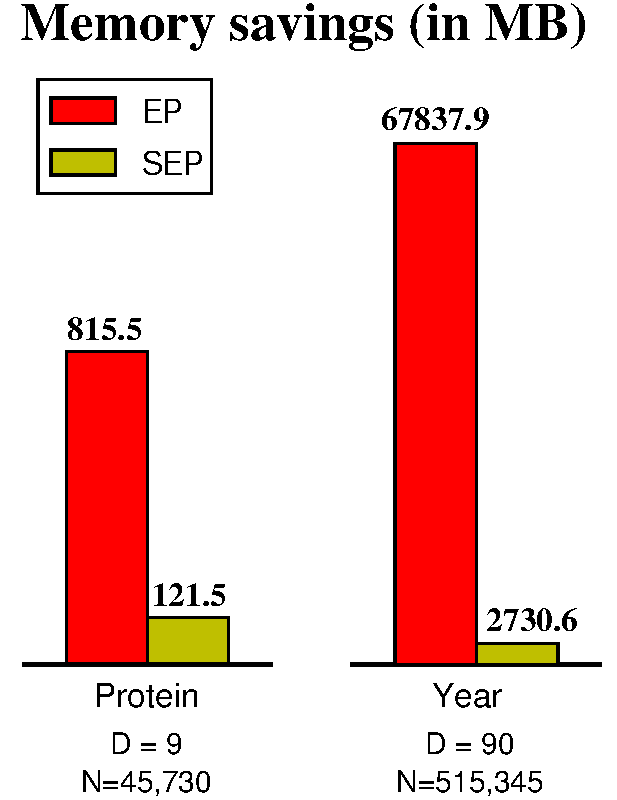
\includegraphics[width=0.4\linewidth]{Chapter3/sep/fig/memory_saving}
\caption{A visualisation of storage savings by SEP.}
\label{fig:chap3_sep_memory_saving}
\end{figure}


\section{Summary}
We have presented the stochastic expectation propagation (SEP) method for reducing EP's large memory consumption that is prohibitive for large datasets. We have connected the new algorithm to a number of existing methods including assumed density filtering, variational message passing, variational inference, stochastic variational inference and averaged EP.
%
Experiments on Bayesian logistic regression (both synthetic and real world) and mixture of Gaussians clustering indicated that the new method had an accuracy that was competitive with EP.  Experiments using the probabilistic back-propagation approach to training Bayesian neural networks on large real world regression datasets again showed that SEP comparably to EP with a vastly reduced memory footprint. 
%

One notable issue that is not addressed here is the theoretical properties of SEP. Does SEP have the same convergence properties as EP in expectation? What is the underlying energy function that SEP is minimising, or is there one at all? in the next chapter we will propose another unifying view of the existing variational methods, but from a very different angle: we will manipulate the energy functions to obtain both upper- and lower-bounds of the marginal likelihood, and discuss connections to VI and EP/SEP with further techniques. Our hope is that, by studying the energy functions, we can get more insights on how EP-like methods work, and better understand the principles of variational methods.


\vspace{1em}
\begin{tcolorbox}
\textbf{Remark} (Further applications of SEP/DSEP)\textbf{.}
The flexibility of the SEP algorithms allow further adjustments of the approximation procedure for different modelling scenarios. For example, we touched on the distributed version of SEP (DSEP) but did not push very far when this work was presented at NIPS 2015. Since then \cite{zhe:yahoo2016} adopted the factor tying idea to develop a highly scalable Bayesian algorithm for online click-through rate prediction on Yahoo! data. In more detail, their idea is DSEP essentially: they maintain the approximating factors for both positive and negative classes, and update them using cheap moment matching techniques. Their experimental results showed that DSEP returns better prediction accuracy compared to widely used algorithms like Vowpal Wabbit\footnote{\url{http://hunch.net/~vw/}} and follow the regularised leader (FTRL)-proximal method \citep{mcmahan:ftrl_proximal2013}.

Another promising direction is the application of SEP algorithms to continual learning \citep{ring:thesis1994, ring:child1997, kirkpatrick:ewc2017}, where information of previous data/task has to be maintained in some way in order to prevent catastrophic forgetting. Indeed the online elastic weight consolidation (EWC) method developed in \cite{schwarz:pc2018} can be viewed as a Laplace approximation version of SEP, which achieves state-of-the-art performance on multiple reinforcement learning tasks.
%
Another interesting idea would combine the \emph{coreset} algorithm with DSEP, where observed data-points in/out of the coreset are handled with different approximating factors.
\end{tcolorbox}

\chapter{R{\'e}nyi Divergence Variational Inference}
\label{chap:vrbound}

% **************************** Define Graphics Path **************************
\ifpdf
    \graphicspath{{Chapter4/Figs/Raster/}{Chapter4/Figs/PDF/}{Chapter4/figs/}}
\else
    \graphicspath{{Chapter4/Figs/Vector/}{Chapter4/figs/}}
\fi


We have discussed in the last chapter a class of EP-like algorithms, which unifies EP, SEP and VI from an algorithmic point of view. Approximate inference is also widely used as a sub-routine in approximate maximum likelihood algorithms and those used for model selections. Historically, VI has received most attentions in this regard. This is mainly because VI has elegant and useful theoretical properties, such as the fact that it proposes a lower-bound of the log-model evidence. 
%
On the other hand, as discussed in the previous chapter, the underlying objective function of SEP is unknown and might not even exist. Even the EP energy itself, although often providing more accurate approximations, has no bounding guarantees \citep{cunningham:gaussianEP2011}. These undesirable issues make EP-like algorithms less appropriate for model selection and approximate MLE. 

To (partially) address these issues, in this chapter we will present a new class of variational inference method using a variant of the $\alpha$-divergences called R{\'e}nyi divergence. We will develop both lower- and upper-bounds to the marginal likelihood, and draw connections to SEP and Black-box-$\alpha$ (introduced by us in \cite{hernandez-lobato:bbalpha2016} but not included in the thesis). This framework is also computationally compelling for Bayesian deep learning, as it is compatible with gradient descent methods (unlike SEP methods which use moment matching). These favourable features are demonstrated with examples including variational auto-encoders and Bayesian neural networks. Throughout the development we will also discuss some theoretical properties of Monte Carlo approximations and data sub-sampling.

%\section{R{\'e}nyi divergences for variational inference}
\label{sec:vrbound_all}

% general idea
%
%%%%%% why VR bound %%%%%%%%
In this section we try to provide a unified framework from an energy function perspective that encompasses a number of recent advances in variational methods, and we hope our effort could potentially motivate new algorithms in the future. This is done by extending traditional VI to R{\'e}nyi's $\alpha$-divergence \cite{renyi:divergence1961}, a rich family that includes many well-known divergences as special cases. After reviewing useful properties of R{\'e}nyi divergences and the VI framework, we make the following contributions:

\begin{itemize}
 \item We introduce the \emph{variational R{\'e}nyi bound} (VR) as an extension of VI/VB. We then discuss connections to existing approaches, including VI/VB, VAE, IWAE \cite{burda:iwae2016}, SEP and BB-$\alpha$, thereby showing the richness of this new family of variational methods.
 %\vspace{-0.03in} 
 \item We develop an optimisation framework for the VR bound. An analysis of the bias introduced by stochastic approximation is also provided with theoretical guarantees and empirical results.
 %\vspace{-0.03in} 
 \item We propose a novel approximate inference algorithm called \emph{VR-max} as a new special case. Evaluations on VAEs and Bayesian neural networks show that this new method is often comparable to, or even better than, a number of the state-of-the-art variational methods.
\end{itemize}

%%%%%%%%% trend of approximate inference %%%%%%%%%%%

\textbf{Remark.} Recent advances of approximate inference follow three major trends. These developments are rather separated and little work has been done to understand their connections, until this section was presented as a conference paper.

First, scalable methods, e.g.~stochastic variational inference (SVI) \cite{hoffman:svi2013} and stochastic expectation propagation (SEP)/AEP \cite{barthelme:aep2015}, have been developed for datasets comprising millions of datapoints. Recent approaches \cite{broderick:stream2013, gelman:dep2014, xu:sms2014} have also applied variational methods to coordinate parallel updates arising from computations performed on chunks of data.

Second, Monte Carlo methods and black-box inference techniques have been deployed to assist variational methods, e.g.~see \cite{paisley:bbvi2012, salimans:reparam2013, ranganath:bbvi2014, kucukelbir:advi2015} for VI and BB-$\alpha$ for EP. They all proposed ascending the Monte Carlo approximated variational bounds to the log-likelihood using noisy gradients computed with automatic differentiation tools.

Third, tighter variational lower-bounds have been proposed for (approximate) MLE. The importance weighted auto-encoder (IWAE) \cite{burda:iwae2016} improved upon the variational auto-encoder (VAE) \cite{kingma:vae2014, rezende:vae2014} framework, by providing tighter lower-bound approximations to the log-likelihood using importance sampling. 
\section{R{\'e}nyi's $\alpha$-divergence}

\label{sec:chap4_vrbound_renyi_divergence}
We first review R{\'e}nyi's $\alpha$-divergence \citep{renyi:divergence1961, van_erven:renyi2014}. R{\'e}nyi's $\alpha$-divergence, defined on $\{\alpha: \alpha > 0, \alpha \neq 1, |\mathrm{D}_{\alpha}^{R}| < +\infty \}$, measures the ``closeness'' of two distributions $p$ and $q$ on a random variable $\bm{\theta} \in \Theta$:
\begin{equation}
\label{eq:renyi_divergence}
\mathrm{D}_{\alpha}^{R} [p || q] = \frac{1}{\alpha - 1} \log \int p(\bm{\theta})^{\alpha} q(\bm{\theta})^{1 - \alpha} d \mu.
\end{equation}
Here the constraint $|D^{R}_{\alpha}[p||q]| < +\infty$ is crucial for rewriting the divergence as the expectation under $p$ or $q$ (i.e. to change the measure from $d\mu$ to $dP$ or $dQ$), i.e. 
$$D_{\alpha}[p||q] = \frac{1}{\alpha - 1} \log \mathbb{E}_{p} \left[ \left( \frac{p(\bm{\theta})}{q(\bm{\theta})}   \right)^{\alpha - 1} \right] = \frac{1}{\alpha - 1} \log \mathbb{E}_{q} \left[ \left( \frac{p(\bm{\theta})}{q(\bm{\theta})}   \right)^{\alpha} \right],$$
since it is possible that the definition (\ref{eq:renyi_divergence}) is infinity but one of the above expectations is finite. In the following we will use $d\mu = d\bm{\theta}$ w.l.o.g.

The definition is extended to $\alpha = 0, 1, +\infty$ by continuity. We note that when $\alpha \rightarrow 1$ the Kullback-Leibler (KL) divergence is recovered, which plays a crucial role in machine learning and information theory. Some other special cases are presented in Table \ref{tab:renyi_example}. The method proposed in this work also considers $\alpha \leq 0$ (although (\ref{eq:renyi_divergence}) is no longer a divergence for these $\alpha$ values), and we include from \cite{van_erven:renyi2014} some useful properties for forthcoming derivations.
%
\begin{prop}
(Monotonicity) R{\'e}nyi's $\alpha$-divergence definition (\ref{eq:renyi_divergence}), extended to negative $\alpha$, is \textbf{continuous} and \textbf{non-decreasing} on $\alpha \in \{\alpha: -\infty < \mathrm{D}_{\alpha}^{R} < +\infty \}$.
\label{prop:renyi_divergence}
\end{prop}
%
\begin{prop}
(Skew symmetry) For $\alpha \not\in \{0, 1\}$, 
$
\mathrm{D}_{\alpha}^{R} [p || q] = \frac{\alpha}{1 - \alpha} \mathrm{D}_{1 - \alpha}^{R} [q || p].
$
This implies $\mathrm{D}_{\alpha}^{R} [p || q] \leq 0$ for $\alpha < 0$. For the limiting case $\mathrm{D}_{-\infty}^{R} [p || q] = -\mathrm{D}_{+\infty}^{R} [q || p]$.
\label{prop:skew_symmetry}
\end{prop}
%
%
\begin{table}[t]
  \centering
  \caption{Special cases in the R{\'e}nyi divergence family.}
  \renewcommand{\arraystretch}{1.2}
  \label{tab:renyi_example}
  \begin{tabular}{ccl}
  	\toprule
    $\alpha$ & Definition & Notes\\
    \hline
    $\alpha \rightarrow 1$ & $\int p(\bm{\theta}) \log \frac{p(\bm{\theta})}{q(\bm{\theta})} d \bm{\theta}$ & 
    \begin{tabular}{@{}l@{}} \emph{Kullback-Leibler (KL) divergence}, \\ used in VI ($\mathrm{KL}[q||p]$) and EP ($\mathrm{KL}[p||q]$) \end{tabular} \\
    %
    $\alpha = 0.5$ & $-2 \log (1 - \mathrm{Hel}^2[p||q])$ & function of the square \emph{Hellinger distance}\\
    %
    $\alpha \rightarrow 0$ & $-\log \int_{p(\bm{\theta}) > 0} q(\bm{\theta}) d\bm{\theta}$ & 
    \begin{tabular}{@{}l@{}} zero when $\mathrm{supp}(q) \subseteq \mathrm{supp}(p)$ \\ (not a divergence) \end{tabular} \\
    %
    $\alpha = 2$ & $-\log (1 - \chi^2[p||q])$ & 
    \begin{tabular}{@{}l@{}} proportional to the $\chi^2$-divergence \end{tabular} \\
    %
    $\alpha \rightarrow +\infty$ & $\log \max_{\bm{\theta} \in \Theta} \frac{p(\bm{\theta})}{q(\bm{\theta})}$ &
    \begin{tabular}{@{}l@{}} \emph{worst-case regret} in \\ \emph{minimum description length principle} \citep{grunwald:mdl2007}\end{tabular} \\
    \bottomrule
  \end{tabular}
  %\vspace{-0.1in}
\end{table}
%
A critical question that is still in active research is how to choose a divergence in this rich family to obtain optimal solution for a particular application, an issue which is discussed in Section \ref{sec:chap4_vrbound_opt_mc}.
\section{Variational R{\'e}nyi bound}
\label{sec:vr_bound}
Recall from previous section that the family of R{\'e}nyi divergences includes the KL divergence. Perhaps variational free-energy approaches can be generalised to the R{\'e}nyi case? Consider approximating the exact posterior $p(\mparam|\mathcal{D})$ by minimizing R{\'e}nyi's $\alpha$-divergence $\mathrm{D}_{\alpha}^{R}[q(\mparam) || p(\mparam | \mathcal{D})]$ for some selected $\alpha > 0$.
%
Now we consider the equivalent optimisation problem 
$$\max_{q \in \mathcal{Q}} \quad  \log p(\mathcal{D}) - \mathrm{D}_{\alpha}^{R}[q(\mparam) || p(\mparam | \mathcal{D})],$$
when $\alpha \neq 1$, the objective can be rewritten as
\begin{equation}
\begin{aligned}
\mathcal{L}_{\alpha}(q; \mathcal{D}) := & \log p(\mathcal{D}) - \mathrm{D}_{\alpha}^{R}[q(\mparam) || p(\mparam | \mathcal{D})] \\
= & \log p(\mathcal{D}) - \frac{1}{\alpha - 1} \log \mathbb{E}_{q} \left[ \left( \frac{q(\mparam) p(\mathcal{D})}{p(\mparam, \mathcal{D})} \right)^{\alpha - 1} \right] \\
= & \frac{1}{1 - \alpha} \log \mathbb{E}_{q} \left[ \left( \frac{p(\mparam, \mathcal{D})}{q(\mparam)} \right)^{1 - \alpha} \right].
\end{aligned}
\label{eq:chap4_vrbound_exact_bound}
\end{equation}
%
We name this new objective the \emph{variational R{\'e}nyi (VR) bound}. Importantly the above definition can be extended to $\alpha \leq 0$, and the following theorem is a direct result of Proposition \ref{prop:renyi_divergence}.
\begin{theorem}
\label{thm:chap4_vrbound_alpha_vi}
The objective $\mathcal{L}_{\alpha}(q; \mathcal{D})$ is \textbf{continuous} and \textbf{non-increasing} on $\alpha \in \{\alpha: |\mathcal{L}_{\alpha}| < +\infty \}$. Especially for all $0 < \alpha_{+} < 1$ and $\alpha_{-} < 0$,
\begin{equation*}
\mathcal{L}_{\text{VI}}(q; \mathcal{D}) = \lim_{\alpha \rightarrow 1} \mathcal{L}_{\alpha}(q; \mathcal{D}) 
 \leq \mathcal{L}_{\alpha_{+}}(q; \mathcal{D}) \leq \mathcal{L}_{0}(q; \mathcal{D}) \leq \mathcal{L}_{\alpha_{-}}(q; \mathcal{D})
\end{equation*}
Also $\mathcal{L}_{0}(q; \mathcal{D}) = \log p(\mathcal{D})$ if and only if the support $ \mathrm{supp}(p(\mparam|\mathcal{D})) \subseteq  \mathrm{supp}(q(\mparam)) $.
\end{theorem}
%
Theorem \ref{thm:chap4_vrbound_alpha_vi} indicates that the VR bound can be useful for model selection by sandwiching the marginal likelihood with bounds computed using positive and negative $\alpha$ values, which we leave to future work. In particular $\mathcal{L}_{0} = \log p(\mathcal{D})$ under the mild assumption that $q$ is supported where the exact posterior is supported. This assumption holds for many commonly used distributions, e.g.~Gaussians are supported on the entire space, and in the following we assume that this condition is satisfied. 

\vspace{1em}
\begin{tcolorbox}
\textbf{Remark} (on marginal likelihood estimation)\textbf{.}
Though not fully discussed in this thesis, it is worth highlighting here the importance of robust marginal likelihood estimation, and thus the usefulness of sandwiching estimates (with both a lower- and an upper-bound). \citet{dieng:chi2016} applied the VR upper-bound to a number of real-world tasks. \cite{grosse:bidirectional2015, grosse:bidirectional2016} proposed bi-directional Monte Carlo method that can be viewed as computing the VR bounds with a sequence of proposal distributions, aiming at reducing the mismatch between $q$ and $p$ thus improving the Monte Carlo estimates. \cite{wu:quantitative2017} applied this idea to perform the first attempt of robust predictive log-likelihood estimation for VAEs and generative adversarial networks (GANs) \citep{goodfellow:gan2014}.   
\end{tcolorbox}
%

\subsection{Mean-field approximation revisited}
\label{sec:chap4_mean_field}

We revisit in the following the mean-field approximation by optimising the VR bound, with Bayesian linear regression as an illustrating example. Recall the mean-field approximation factorises over the components of $\mparam = (\theta_1, ..., \theta_D)$: $q(\mparam) = \prod_{i} q_i(\theta_i)$. Re-writing the VR bound (\ref{eq:chap4_vrbound_exact_bound}), we have
\begin{equation*}
\begin{aligned}
\mathcal{L}_{\alpha}(q; \mathcal{D}) &= \frac{1}{1 - \alpha} \log \int \prod_i q_i(\theta_i)  \left( \frac{p(\mparam, \mathcal{D})}{\prod_i q_i(\theta_i)} \right)^{1 - \alpha} d\mparam \\
&= \frac{1}{1 - \alpha} \log \int q_j(\theta_j)^{\alpha} \left( \int \prod_{i \neq j} q_i(\theta_i)  \left( \frac{p(\mparam, \mathcal{D})}{\prod_{i \neq j} q_i(\theta_i)} \right)^{1 - \alpha} d\mparam_{\neq j} \right) d\theta_j \\
&:= \frac{1}{1 - \alpha} \log \int q_j(\theta_j)^{\alpha} \tilde{p}_j(\theta_j)^{1 - \alpha} d\theta_j + \text{const},
\end{aligned}
\end{equation*}
where $\tilde{p}_j(\theta_j)$ denote the ``marginal'' distribution satisfying
\begin{equation*}
\log \tilde{p}_j(\theta_j) = \frac{1}{1 - \alpha} \log \int \prod_{i \neq j} q_i(\theta_i)  \left( \frac{p(\mparam, \mathcal{D})}{\prod_{i \neq j} q_i(\theta_i)} \right)^{1 - \alpha} d\mparam_{\neq j} + \text{const}.
\end{equation*}
Now maximising the VR bound (when $\alpha > 0$, and for $\alpha < 0$ we minimise the bound) is equivalent to minimising $\mathrm{D}_{\alpha}^{R}[q_j||\tilde{p}_j]$ (for $\alpha > 0$, and when $\alpha < 0$ we minimise $\mathrm{D}_{1 - \alpha}^{R}[\tilde{p}_j||q_j]$), which means $\log q_j(\theta_j) = \log \tilde{p}_j(\theta_j) + \text{const}$ is the only global optimum of the mean-field approximation procedure. One can verify that when $\alpha \rightarrow 1$ it recovers the traditional variational mean-field approximation (see Section \ref{sec:chap2_mean_field_vi})
\begin{equation*}
\lim_{\alpha \rightarrow 1} \log \tilde{p}_j(\theta_j) = \int \prod_{i \neq j} q_i(\theta_i) \log p(\mparam, \mathcal{D}) d\mparam_{\neq j} + \text{const},
\end{equation*}
and when $\alpha \rightarrow 0$ the fixed point equation returns the exact marginal of the posterior distribution:\footnote{This is \emph{not} the unique fixed point of $\lim_{\alpha \rightarrow 0} \mathcal{L}_{\alpha} = \mathcal{L}_0$, since $\mathcal{L}_0 = \text{const}$ when $q$ has full support.} 
$$\lim_{\alpha \rightarrow 0} \tilde{p}_j(\theta_j) = p(\theta_j |\mathcal{D}).$$

Now consider Bayesian linear regression with 2-D input $\bm{x}$ and 1-D output $y$, as an example:
\begin{equation*}
\mparam \sim \mathcal{N}(\mparam; \bm{\mu}_0, \bm{\Lambda}_0^{-1}), \quad 
y|\bm{x} \sim \mathcal{N}(y; \mparam^T \bm{x}, \sigma^2).
\end{equation*}
Given the observations $\mathcal{D} = \{\bm{x}_n, y_n \}$, the posterior distribution of $\mparam$ can be computed analytically as $p(\mparam|\mathcal{D}) = \mathcal{N}(\mparam; \bm{\mu}, \bm{\Lambda}^{-1})$ with $\bm{\Lambda} = \bm{\Lambda}_0 + \frac{1}{\sigma^2} \sum_n \bm{x}_n \bm{x}_n^T$ and $\bm{\Lambda} \bm{\mu} = \bm{\Lambda}_0 \bm{\mu}_0 + \frac{1}{\sigma^2} \sum_n y_n \bm{x}_n$. To see how the mean-field approach works we explicitly write down the elements of the posterior parameters
\begin{equation*}
\bm{\mu} = \begin{pmatrix} \mu_1 \\ \mu_2 \end{pmatrix}, \quad
\bm{\Lambda} = \begin{pmatrix} \Lambda_{11} & \Lambda_{12} \\ \Lambda_{21} & \Lambda_{22} \end{pmatrix}, 
\quad \Lambda_{12} = \Lambda_{21},
\end{equation*}
and define $q_i(\theta_i) = \mathcal{N}(\theta_i; m_i, \lambda_i^{-1})$ as a univariate Gaussian distribution. Then
\begin{equation*}
\begin{aligned}
\log q_1 &= \frac{1}{1 - \alpha} \log \int q_2(\theta_2)  \left( \frac{p(\mparam, \mathcal{D})}{q_2(\theta_2)} \right)^{1 - \alpha} d\theta_2 + \text{const} \\
&= \frac{1}{1 - \alpha} \log \int \exp \left[ -\frac{1 - \alpha}{2} (\mparam - \bm{\mu})^T \bm{\Lambda} (\mparam - \bm{\mu}) - \frac{\alpha}{2} \lambda_2 (\theta_2 - m_2)^2 \right] d\theta_2 + \text{const} \\
&= \frac{1}{1 - \alpha} \log \int \mathcal{N}(\mparam; \bm{\mu}, \tilde{\bm{\Sigma}}) d\theta_2 + \text{const} \\
&= \log \mathcal{N}(\theta_1; m_1, \lambda^{-1}) + \text{const}
\end{aligned}
\end{equation*}
where the new mean $m_1$ and the precision $\lambda_1$ satisfies
\begin{equation*}
\begin{aligned}
m_1 = \mu_1 + C_1(\mu_2 - m_2), \quad C_1 = \frac{\alpha \lambda_2 \Lambda_{12}}{(1 - \alpha) |\bm{\Lambda}| + \alpha \lambda_2 \Lambda_{11}}, \\
\lambda_1 = \Lambda_{11} - (1 - \alpha) \Lambda_{12} ((1 - \alpha) \Lambda_{22} + \alpha \lambda_2)^{-1} \Lambda_{21}.
\end{aligned}
\end{equation*}
One can derive the terms $m_2$ and $C_2$ for $q_2$ in the same way, and show that $\bm{m} = \bm{\mu}$ is the only stable fixed point of this iterative update. So we have $q_1 = \mathcal{N}(\theta_1; \mu_1, \lambda_1^{-1})$, and similarly $q_2 = \mathcal{N}(\theta_1; \mu_2, \lambda_2^{-1})$ with $\lambda_2 = \Lambda_{22} - (1 - \alpha) \Lambda_{21} ((1 - \alpha) \Lambda_{11} + \alpha \lambda_1)^{-1} \Lambda_{12}$. In this example $\lambda_1$, $\lambda_2$ are feasible for all $\alpha$, and solving the fixed point equations, finally we have the stable fixed point as
\begin{equation*}
\lambda_1 = \rho_{\alpha} \Lambda_{11}, \quad \lambda_2 = \rho_{\alpha} \Lambda_{22}, \quad 
\rho_{\alpha} = \frac{1}{2 \alpha} \left[ (2\alpha - 1) + \sqrt{1 - \frac{4\alpha (1 - \alpha) \Lambda_{12}^2}{\Lambda_{11} \Lambda_{22}}} \right].
\end{equation*}
The other solution for the quadratic formula is eliminated since it violates the assumptions that $\lambda_1 > 0$ (when $0 < \alpha < 1$) and $|\mathcal{L}_{\alpha}| < +\infty$ (when $\alpha < 0$ or $\alpha > 1$, since it requires $|\alpha \text{diag}(\bm{\lambda}) + (1 - \alpha)\bm{\Lambda}| > 0$). Thus the stable fixed point in this case is unique.

One can show that $\lim_{\alpha \rightarrow 1} \lambda_1 = \Lambda_{11}$ (the precision of the conditional distribution $p(\theta_1 | \theta_2, \data)$), $\lim_{\alpha \rightarrow 0} \lambda_1 = \Lambda_{11} - \Lambda_{12} \Lambda_{22}^{-1} \Lambda_{21}$ (the precision of the marginal distribution $p(\theta_1|\data)$), and $\lim_{\alpha \rightarrow \pm \infty} \lambda_1 = \Lambda_{11} \pm |\Lambda_{12}| \sqrt{\Lambda_{11} \Lambda_{22}^{-1}}$ (similar results for $\lambda_2$). Also $\rho_{\alpha}$ is continuous and non-decreasing in $\alpha$. This means one can interpolate between mass-covering ($\alpha \rightarrow -\infty$) and zero-forcing ($\alpha \rightarrow +\infty$, when using uni-modal approximations it is usually called mode-seeking) behaviour by increasing $\alpha$ values. 

We visualise the analytical results for Bayesian linear regression in Figure \ref{fig:chap4_vrbound_linear_regression_posterior} and  \ref{fig:chap4_vrbound_linear_regression_energy}. First as predicted, increasing $\alpha$ returns more confident estimate. Also notice that $\alpha \rightarrow +\infty$ (in cyan) returns non-zero uncertainty estimates (although it is more over-confident than VI) which is different from the maximum a posteriori (MAP) method that only returns a point estimate. Second, setting $\alpha = 0.0$ (in green) returns $q(\mparam) = \prod_i p(\theta_i|\mathcal{D})$ and the exact marginal likelihood $\log p(\mathcal{D})$ (Figure \ref{fig:chap4_vrbound_linear_regression_energy}). Also the approximate MLE is less biased for $\alpha = 0.5$ (in blue) since now the tightness of the bound is less hyper-parameter dependent.

\begin{figure}[t]
 \centering
 \subfigure[Approximated posterior.]{
 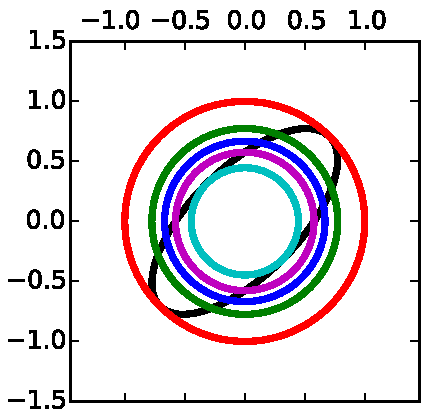
\includegraphics[width=0.24\linewidth]{Chapter4/figs/approx.pdf}
 \label{fig:chap4_vrbound_linear_regression_posterior}}
 \hspace{0.5in}
 \subfigure[Hyper-parameter optimisation.]{
 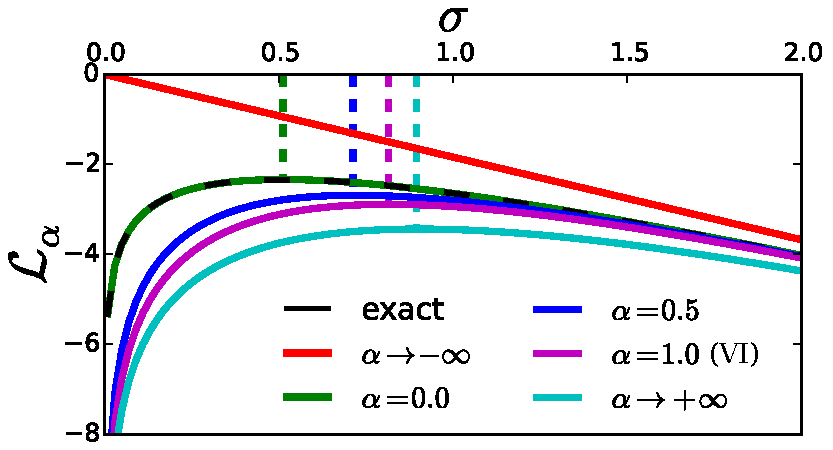
\includegraphics[width=0.45\linewidth]{Chapter4/figs/log_evidence.pdf}
 \label{fig:chap4_vrbound_linear_regression_energy}}
 \caption{Mean-Field approximation for Bayesian linear regression (with one-sigma contours). C.f. Figure \ref{fig:chap2_mean_field}. In this case $\bm{\varphi} = \sigma$ the observation noise variance. As expected when $\alpha = 0$ the resulting bound coincides with the exact log marginal (see the green-black curve). The bound is tight as $\sigma \rightarrow +\infty$, biasing the VI solution to large $\sigma$ values.}
\end{figure}


\subsection{Monte Carlo approximation of the VR bound}
\label{sec:chap4_vrbound_sampling}

Although we have seen some nice properties of the VR bound optimisation through the mean-field approximation example, we also note that when $\alpha \neq 1$, the VR bound is usually just as intractable as the marginal likelihood for many other useful models. Also Theorem \ref{thm:chap4_vrbound_alpha_vi} suggests that the VR bound is to be minimised when $\alpha < 0$, which performs disastrously in MLE context.
%
 As we shall see, these issues are addressed by the MC approximation that we will be developing as follows, under certain conditions. Therefore, MC-VR can be applied to precisely the same set of models as MC-VI \citep{paisley:bbvi2012, salimans:reparam2013, ranganath:bbvi2014, kucukelbir:advi2015}.

Consider learning a latent variable model with MLE as a running example, where the model is specified by a conditional distribution $p(\bm{x}|\z, \bm{\varphi})$ and a prior $p(\z| \bm{\varphi})$ on the latent variable $\z$. Examples include latent variable models treated by the variational auto-encoder (VAE) approach \citep{kingma:vae2014, rezende:vae2014} that parametrises the likelihood with a (deep) neural network. MLE requires $\log p(\bm{x})$ which is obtained by marginalising out $\z$ and is often intractable, so the VR bound is considered as an alternative optimisation objective. However instead of using exact bounds, a simple Monte Carlo (MC) method is deployed, which uses a finite number of samples $\z_k \sim q(\z|\bm{x}), k = 1, ..., K$ to approximate the VR bound $\mathcal{L}_{\alpha} \approx \hat{\mathcal{L}}_{\alpha, K}$:
\begin{equation}
\label{eq:sampling_estimate}
\hat{\mathcal{L}}_{\alpha, K}(q; \bm{x}) = \frac{1}{1 - \alpha} \log \frac{1}{K} \sum_{k=1}^K \left[\left( \frac{p(\z_k, \bm{x})}{q(\z_k|\bm{x})} \right)^{1 - \alpha} \right].
\end{equation}
The importance weighted auto-encoder (IWAE) \citep{burda:iwae2016} is a special case of this framework with $\alpha = 0$ and $K < +\infty$. But unlike traditional VI, here the MC approximation is biased. Fortunately we can characterise the bias by the following theorems (proofs provided in Appendix \ref{sec:appendix_proof_chap4}).
%
%
%%%%% theorem %%%%%
\begin{theorem}
\label{thm:chap4_vrbound_sampling_bound}
Assume $\mathbb{E}_{\{\z_k\}_{k=1}^K} [ |\hat{\mathcal{L}}_{\alpha, K}(q; \bm{x})| ] < + \infty$ and $|\mathcal{L}_{\alpha}| < +\infty$. Then $\mathbb{E}_{\{\z_k\}_{k=1}^K} [ \hat{\mathcal{L}}_{\alpha, K}(q; \bm{x}) ]$ as a function of $\alpha \in \mathbb{R}$ and $K \geq 1$ is: \\
1) \textbf{non-decreasing} in $K$ for fixed $\alpha \leq 1$, and \textbf{non-increasing} in $K$ for fixed $\alpha \geq 1$; \\
2) $\mathbb{E}_{\{\z_k\}_{k=1}^K} [ \hat{\mathcal{L}}_{\alpha, K}(q; \bm{x}) ] \rightarrow \mathcal{L}_{\alpha}$ as $K \rightarrow +\infty$; \\
3) \textbf{continuous} and \textbf{non-increasing} in $\alpha$ with fixed $K$.
\end{theorem}

%%%%%% corollary %%%%%
\begin{corollary}
\label{thm:chap4_vrbound_alpha_k_existence}
For finite $K$, either $\mathbb{E}_{\{\z_k\}_{k=1}^K} [ \hat{\mathcal{L}}_{\alpha, K}(q; \bm{x}) ] < \log p(\bm{x})$ for all $\alpha$, or there exists $\alpha_K \leq 0$ such that $\mathbb{E}_{\{\z_k\}_{k=1}^K} [ \hat{\mathcal{L}}_{\alpha_K, K}(q; \bm{x}) ] = \log p(\bm{x})$ and $\mathbb{E}_{\{\z_k\}_{k=1}^K} [ \hat{\mathcal{L}}_{\alpha, K}(q; \bm{x}) ] > \log p(\bm{x})$ for all $\alpha < \alpha_K$. Also $\alpha_K$ is \textbf{non-decreasing} in $K$ if exists, with $\lim_{K \rightarrow 1} \alpha_K = -\infty$ and $\lim_{K \rightarrow +\infty} \alpha_K = 0$.
\end{corollary}
%%%%%%%%%%%%%%%%

%
The intuition behind the theorems is visualised in Figure \ref{fig:chap4_vrbound_divergence_sampling}. By definition, the exact VR bound is a lower-bound or upper-bound of $\log p(\bm{x})$ when $\alpha > 0$ or $\alpha < 0$, respectively. However the MC approximation $\mathbb{E}[\hat{\mathcal{L}}_{\alpha, K}]$ biases the estimate towards $\mathcal{L}_{\text{VI}}$, where the MC approximation of the bound can be improved using more samples. Thus for finite samples and under mild conditions, negative alpha values can potentially be used to improve the accuracy of the approximation, although the MC approximation for these alpha values is no longer guaranteed to be an upper bound.
%
Figure \ref{fig:chap4_vrbound_divergence_simulation} shows an empirical evaluation by computing the exact and the MC approximation of the R{\'e}nyi divergence. In this example $p$, $q$ are 2-D Gaussian distributions with $\bm{\mu}_p = [0, 0]$, $\bm{\mu}_q = [1, 1]$ and $\bm{\Sigma}_p = \bm{\Sigma}_q = \bm{I}$. The sampling procedure is repeated 200 times to estimate the expectation. Clearly for $K = 1$ it is equivalent to an unbiased estimate of the KL-divergence for all $\alpha$ (even though now the estimation is biased for $\mathrm{D}_{\alpha}^{R}$). For $K > 1$ and $\alpha < 1$, the MC method under-estimates the VR bound, and the bias decreases with increasing $K$. For $\alpha > 1$ the inequality is reversed also as predicted.


\begin{figure*}[t]
 \centering
 \subfigure[MC approximated VR bounds.]{
 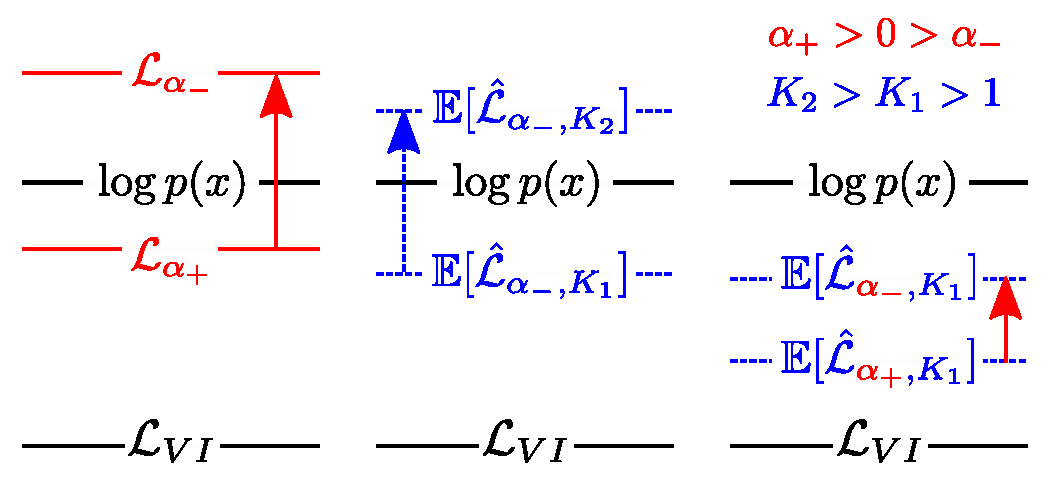
\includegraphics[width=0.6\linewidth]{sampling_bound_full.pdf}
 \label{fig:chap4_vrbound_divergence_sampling}}
 \hspace{0.1in}
 \subfigure[Simulated MC approximations.]{
 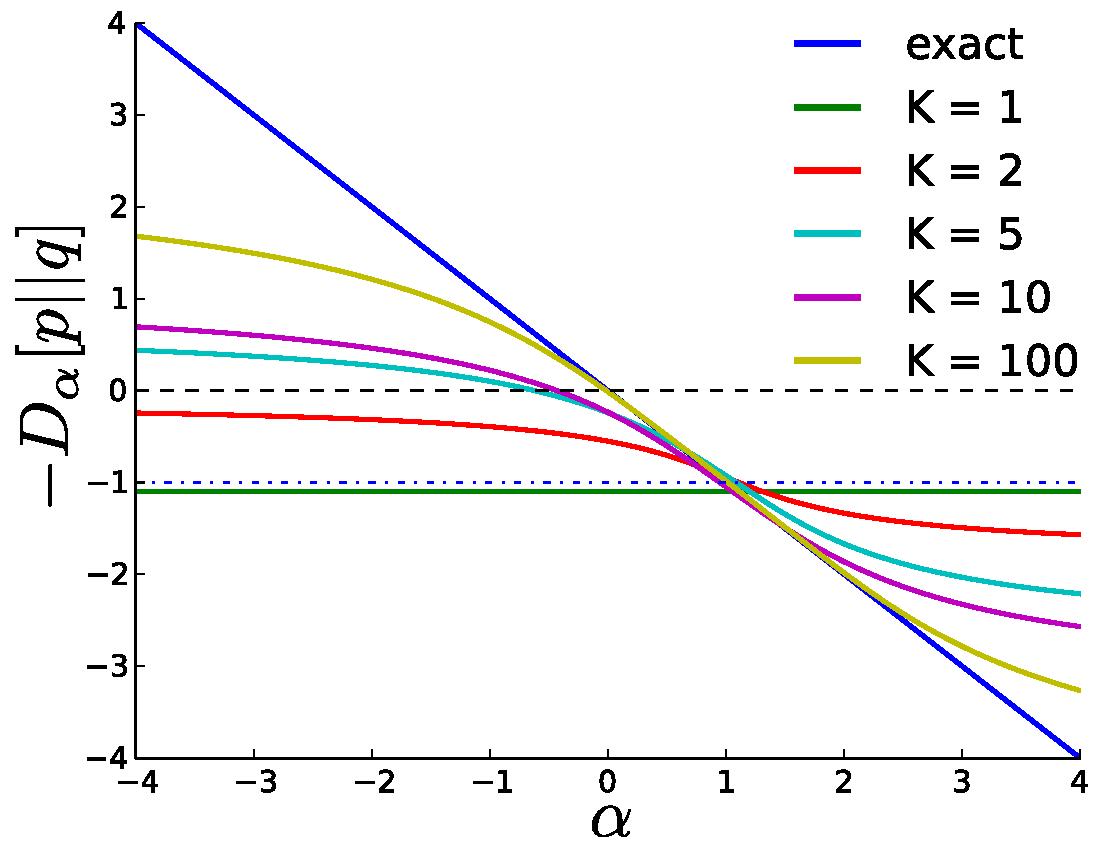
\includegraphics[width=0.34\linewidth]{divergence_sampling.pdf}
 \label{fig:chap4_vrbound_divergence_simulation}}
 \vspace{-0.1in}
 \caption{(a) An illustration for the bounding properties of MC approximations to the VR bounds (non-increasing in $\alpha$ and non-decreasing in $K$ when $\alpha \leq 1$). (b) The bias of the MC approximation, where the dash-dotted line on top of the green line ($K=1$) is the analytical value of $-\mathrm{KL}[p||q]$. Best viewed in colour and see the main text for details.}
\end{figure*}
%%%%%%%%%%%%%%%%%%%%
\subsection{A unified implementation with the reparameterisation trick}

Readers may have noticed that $\mathcal{L}_{\text{VI}}$ has a different form compared to $\mathcal{L}_{\alpha}$ with $\alpha \neq 1$. In this section we show how to unify the implementation for all finite $\alpha$ settings using the \emph{reparameterisation trick} \citep{salimans:reparam2013, kingma:vae2014} as an example. This trick assumes the existence of the mapping $\bm{\theta} = g_{\bm{\phi}}(\bm{\epsilon})$, where the distribution of the noise term $\bm{\epsilon}$ satisfies $q(\bm{\theta}) d\bm{\theta} = p(\bm{\epsilon}) d\bm{\epsilon}$. Then the expectation of a function $F(\bm{\theta})$ over distribution $q(\bm{\theta})$ can be computed as
%
$\mathbb{E}_{q(\bm{\theta})} [F(\bm{\theta})] = \mathbb{E}_{p(\bm{\epsilon})} [F(g_{\bm{\phi}}(\bm{\epsilon}))].$
%
One prevalent example is the Gaussian reparameterisation: $\bm{\theta} \sim \mathcal{N}(\bm{\mu}, \Sigma) \Rightarrow \bm{\theta} = \bm{\mu} + \Sigma^{ \frac{1}{2} } \bm{\epsilon}$, with $\bm{\epsilon} \sim \mathcal{N}(\bm{0}, I)$. 
%
Now we apply the reparameterisation trick to the VR bound
%
\begin{equation}
\mathcal{L}_{\alpha}(q_{\bm{\phi}}; \bm{x}) = \frac{1}{1 - \alpha} \log \mathbb{E}_{\bm{\epsilon}} \left[\left( \frac{p(g_{\bm{\phi}}(\bm{\epsilon}) , \bm{x})}{q(g_{\bm{\phi}}(\bm{\epsilon}))} \right)^{1 - \alpha} \right].
\end{equation}
%
For notational ease we also write $g_{\bm{\phi}} = g_{\bm{\phi}}(\bm{\epsilon})$. Then the gradient of the VR bound w.r.t.~$\bm{\phi}$ (similar for $\bm{\varphi}$) is
\begin{equation}
\begin{aligned}
\nabla_{\bm{\phi}} \mathcal{L}_{\alpha}(q_{\bm{\phi}}; \bm{x}) 
&= \frac{1}{1 - \alpha} \nabla_{\bm{\phi}} \log \mathbb{E}_{\bm{\epsilon}} \left[ \left( \frac{p(g_{\bm{\phi}}, \bm{x})}{q(g_{\bm{\phi}})} \right)^{1 - \alpha} \right] \\
&= \frac{1}{1 - \alpha} \left( \mathbb{E}_{\bm{\epsilon}} \left[ \left( \frac{p(g_{\bm{\phi}}, \bm{x})}{q(g_{\bm{\phi}})} \right)^{1 - \alpha} \right] \right)^{-1} \mathbb{E}_{\bm{\epsilon}} \left[ \nabla_{\bm{\phi}} \left( \frac{p(g_{\bm{\phi}}, \bm{x})}{q(g_{\bm{\phi}})} \right)^{1 - \alpha} \right] \\
&= \frac{1}{1 - \alpha} \left( \mathbb{E}_{\bm{\epsilon}} \left[ \left( \frac{p(g_{\bm{\phi}}, \bm{x})}{q(g_{\bm{\phi}})} \right)^{1 - \alpha} \right] \right)^{-1} \mathbb{E}_{\bm{\epsilon}} \left[ \left( \frac{p(g_{\bm{\phi}}, \bm{x})}{q(g_{\bm{\phi}})} \right)^{1 - \alpha} \nabla_{\bm{\phi}} (1 - \alpha) \log \frac{p(g_{\bm{\phi}}, \bm{x})}{q(g_{\bm{\phi}})} \right] \\
&= \mathbb{E}_{\bm{\epsilon}} \left[ w_{\alpha}(\bm{\epsilon}; \bm{\phi}, \bm{x}) \nabla_{\bm{\phi}} \log \frac{p(g_{\bm{\phi}}, \bm{x})}{q(g_{\bm{\phi}})} \right].
\end{aligned}
\label{eq:chap4_vrbound_gradient_reparam}
\end{equation}
%
where $w_{\alpha}(\bm{\epsilon}; \bm{\phi}, \bm{x}) = \left( \frac{p(g_{\bm{\phi}}(\bm{\epsilon}), \bm{x})}{q(g_{\bm{\phi}}(\bm{\epsilon}))} \right)^{1 - \alpha} \bigg/ \mathbb{E}_{\bm{\epsilon}} \left[ \left( \frac{p(g_{\bm{\phi}}(\bm{\epsilon}), \bm{x})}{q(g_{\bm{\phi}}(\bm{\epsilon}))} \right)^{1 - \alpha} \right]$ denotes the normalised importance weight. 
%
One can show that this recovers the the stochastic gradients of $\mathcal{L}_{\text{VI}}$ by setting $\alpha = 1$ in (\ref{eq:chap4_vrbound_gradient_reparam}) since now $w_{1}(\bm{\epsilon}; \bm{\phi}, \bm{x}) = 1$, which means the resulting algorithm unifies the computation for all finite $\alpha$ settings. For MC approximations, we use $K$ samples to approximately compute the weight $\hat{w}_{\alpha, k}(\bm{\epsilon}_k; \bm{\phi}, \bm{x}) \propto \left( \frac{p(g_{\bm{\phi}}(\bm{\epsilon}_k), \bm{x})}{q(g_{\bm{\phi}}(\bm{\epsilon}_k))} \right)^{1 - \alpha}$, $k = 1, ..., K$, and the stochastic gradient becomes
\begin{equation}
\nabla_{\bm{\phi}} \hat{\mathcal{L}}_{\alpha, K}(q_{\bm{\phi}}; \bm{x}) 
= \sum_{k=1}^K \left[ \hat{w}_{\alpha, k}(\bm{\epsilon}_k; \bm{\phi}, \bm{x}) \nabla_{\bm{\phi}} \log \frac{p(g_{\bm{\phi}}(\bm{\epsilon}_k), \bm{x})}{q(g_{\bm{\phi}}(\bm{\epsilon}_k))} \right].
\end{equation}
When $\alpha = 1$, $\hat{w}_{1, k}(\bm{\epsilon}_k; \bm{\phi}, \bm{x}) = 1/K$, and it recovers the stochastic gradient VI method \citep{kingma:vae2014}.

To speed-up learning \citet{burda:iwae2016} suggested back-propagating only one sample $\bm{\epsilon}_j$ with $j \sim p_j = \hat{w}_{\alpha, j}$, which can be easily extended to our framework. Importantly, the use of different $\alpha < 1$ indicates the degree of emphasis placed upon locations where the approximation $q$ under-estimates $p$, and in the extreme case $\alpha \rightarrow -\infty$, the algorithm chooses the sample that has the \emph{maximum} unnormalised importance weight. 
%
We name this approach \emph{VR-max} and summarise it and the general case in Algorithm \ref{alg:vr_max}. 
%
Note that VR-max (and VR-$\alpha$ with $\alpha < 0$ and MC approximations) does \emph{not} minimise $\mathrm{D}_{1-\alpha}^{R}[p||q]$. It is true that $\mathcal{L}_{\alpha} \geq \log p(\bm{x})$ for negative $\alpha$ values. However Corollary \ref{thm:chap4_vrbound_alpha_k_existence} suggests that the tightest MC approximation for given $K$ has non-positive $\alpha_K$ value, or might not even exist. Furthermore the optimal $\alpha_K$ value becomes more negative as the mismatch between $q$ and $p$ increases, e.g.~the VAE uses a uni-modal $q$ distribution to approximate the typically multi-modal exact posterior.



\begin{figure}[!t]
% UGLY USE OF \vspace & \hspace follows
\begin{minipage}[b]{0.55\linewidth}
\centering
\begin{algorithm}[H] 
\caption{One gradient step for VR-$\alpha$/VR-max with single backward pass. Here $\hat{w}(\bm{\epsilon}_k; \bm{x})$ short-hands $\hat{w}_{0, k}(\bm{\epsilon}_k; \bm{\phi}, \bm{x})$ in the main text.} \small
\label{alg:vr_max} 
\begin{algorithmic}[1] 
	\STATE given the current datapoint $\bm{x}$, sample \\$\bm{\epsilon}_1, ..., \bm{\epsilon}_K \sim p(\bm{\epsilon})$
	\STATE for $k = 1, ..., K$, compute the unnormalised weight \\
	$\log \hat{w}(\bm{\epsilon}_k; \bm{x}) = \log p(g_{\bm{\phi}}(\bm{\epsilon}_k), \bm{x}) - \log q(g_{\bm{\phi}}(\bm{\epsilon}_k)|\bm{x})$
	\STATE choose the sample $\bm{\epsilon}_{j}$ to back-propagate: \\
	if $|\alpha| < \infty$: $j \sim p_k$ where $p_k \propto \hat{w}(\bm{\epsilon}_k; \bm{x})^{1 - \alpha}$ \\
	if $\alpha = -\infty$: $j = \argmax_{k} \log \hat{w}(\bm{\epsilon}_k; \bm{x})$ 
	\STATE return the gradients $\nabla_{\bm{\phi}} \log \hat{w}(\bm{\epsilon}_{j}; \bm{x})$
\end{algorithmic}
\end{algorithm}
\end{minipage}
%
\hfill
\begin{minipage}[b]{0.4\linewidth}
\centering
 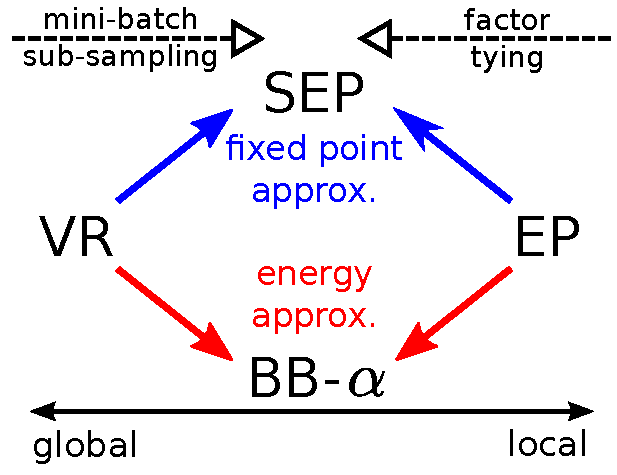
\includegraphics[width=0.9\linewidth]{vr_ep_relationship.pdf} 
 \vspace{-0.1in}
 \captionof{figure}{Connecting local and global divergence minimisation.}
 \label{fig:vr_ep_relationship}
\end{minipage}
%\quad
%
\end{figure}


%%%%%%%%%%%%%%
\subsection{Stochastic approximation for large-scale learning}
\label{sec:chap4_vrbound_large_scale_learning}
VR bounds can also be applied to full Bayesian inference with posterior approximation. However for large datasets full batch learning is very inefficient. Mini-batch training is non-trivial here since the VR bound cannot be represented by the expectation of a datapoint-wise loss, except when $\alpha = 1$ (VI). This section introduces two proposals for mini-batch training, and interestingly, this recovers two existing algorithms that were motivated from a different perspective.
%
In the following we define the (geometric) ``average likelihood'' $\bar{f}_{\mathcal{D}}(\bm{\theta}) = [\prod_{n=1}^N p(\bm{x}_n|\bm{\theta})]^{\frac{1}{N}}$. Hence the joint distribution can be rewritten as $p(\bm{\theta}, \mathcal{D}) = p_0(\bm{\theta}) \bar{f}_{\mathcal{D}}(\bm{\theta})^N$. Also for a mini-batch of $M$ datapoints $\mathcal{S} = \{\bm{x}_{n_1}, ..., \bm{x}_{n_M} \} \sim \mathcal{D}$, we define the ``subset average likelihood'' $\bar{f}_{\mathcal{S}}(\bm{\theta}) = [\prod_{m=1}^M p(\bm{x}_{n_m}|\bm{\theta})]^{\frac{1}{M}}$.

The first proposal considers \emph{fixed point approximations} with mini-batch sub-sampling. It first derives the fixed point conditions for the variational parameters (e.g.~the natural parameters of $q$) using the exact VR bound (\ref{eq:chap4_vrbound_exact_bound}), then designs an iterative algorithm using those fixed point equations, but with $\bar{f}_{\mathcal{D}}(\bm{\theta})$ replaced by $\bar{f}_{\mathcal{S}}(\bm{\theta})$.
%
The second proposal also applies this subset average likelihood approximation idea, but directly to the VR bound (\ref{eq:chap4_vrbound_exact_bound}) (so this approach is named \emph{energy approximation}):
\begin{equation}
\label{eq:alpha_vi_approx}
\tilde{\mathcal{L}}_{\alpha}(q; \mathcal{S}) 
	= \frac{1}{1 - \alpha} \log \mathbb{E}_{q} \left[ \left( \frac{p_0(\bm{\theta}) \bar{f}_{\mathcal{S}}(\bm{\theta})^N} {q(\bm{\theta})} \right)^{1 - \alpha} \right].
\end{equation}
%
Now we demonstrate with detailed derivations that fixed point approximation returns stochastic EP (SEP, see Chapter \ref{chap:factor_tying}) , and black box alpha (BB-$\alpha$) \citep{hernandez-lobato:bbalpha2016} corresponds to energy approximation. We derive the results in exponential family context, but in general these two principles of stochastic approximation also apply. Note that both methods use Minka's $\alpha$-divergence, and for clear distinction here we use $\beta$ instead to denote the corresponding $\alpha$ values for Minka's definition, and hence the two algorithms are returned respectively by taking $M = 1$ and $\alpha = 1 - \beta/N$.

Precisely, we assume the posterior approximation is defined as $q(\bm{\theta}) = \frac{1}{Z_q} p_0(\bm{\theta}) t(\bm{\theta})^N$.
Often $t(\bm{\theta})$ is chosen to have an exponential family form $t(\bm{\theta}) \propto \exp \left[ \langle \bm{\lambda}, \bm{\Phi}(\bm{\theta}) \rangle \right]$ with $\bm{\Phi}(\bm{\theta})$ denoting the sufficient statistic. Then picking $\alpha = 1 - \beta/N$, $\beta \neq 0$, we obtain the exact VR bound (by pulling out the normalising constant $Z_q$) as
\begin{equation}
\mathcal{L}_{\alpha}(q; \mathcal{D}) = \log Z_q + \frac{N}{\beta} \log \mathbb{E}_{q} \left[ \left( \frac{ \bar{f}_{\mathcal{D}}(\bm{\theta})} {t(\bm{\theta})} \right)^{\beta} \right].
\label{eq:vr_bound_sa_exact}
\end{equation}

The first proposal considers deriving the exact fixed point conditions, then approximating them with mini-batch sub-sampling. In our example the exact fixed point condition for the variational parameters $\bm{\lambda}$ is
\begin{equation}
\nabla_{\bm{\lambda}} \mathcal{L}_{\alpha}(q; \mathcal{D}) = 0 \quad \Rightarrow \quad \mathbb{E}_{q}[\bm{\Phi}(\bm{\theta})] = \mathbb{E}_{\tilde{p}_{\alpha}}[\bm{\Phi}(\bm{\theta})],
\end{equation} 
with the tilted distribution defined as 
$$\tilde{p}_{\alpha}(\bm{\theta}) \propto q(\bm{\theta})^{\alpha}p_0(\bm{\theta})^{1 - \alpha} \bar{f}_{\mathcal{D}}(\bm{\theta})^{N(1 - \alpha)} \propto p_0(\bm{\theta}) t(\bm{\theta})^{N - \beta} \bar{f}_{\mathcal{D}}(\bm{\theta})^{\beta}.$$ 
Now given a mini-batch of datapoints $\mathcal{S}$, the moment matching update can be approximated by replacing $\bar{f}_{\mathcal{D}}(\bm{\theta})$ with $\bar{f}_{\mathcal{S}}(\bm{\theta}) = [\prod_{m=1}^M p(\bm{x}_{n_m}|\bm{\theta})]^{\frac{1}{M}}$. More precisely, each iteration we sample a subset of data $\mathcal{S} = \{\bm{x}_{n_1}, ..., \bm{x}_{n_M} \} \sim \mathcal{D}$, and compute the new update for $\bm{\lambda}$ by first computing $\tilde{p}_{\alpha, \mathcal{S}}(\bm{\theta}) \propto p_0(\bm{\theta}) t(\bm{\theta})^{N - \beta} \bar{f}_{\mathcal{S}}(\bm{\theta})^{\beta}$ then taking $\mathbb{E}_{q}[\bm{\Phi}(\bm{\theta})] \leftarrow \mathbb{E}_{\tilde{p}_{\alpha, \mathcal{S}}}[\bm{\Phi}(\bm{\theta})]$. This method returns SEP when $M = 1$, i.e.~in each iteration only one datapoint is sampled to update the approximate posterior. Using larger mini-batch size $M > 1$ returns SDEP (see Section \ref{sec:chap3_sep_dep}) and in this case further approximation might be required to compute the fixed point iterative updates.

%
The second proposal also applies this subset average likelihood approximation idea, but directly to the VR bound (\ref{eq:vr_bound_sa_exact}), with $\mathbb{E}_{\mathcal{S}}$ denoting the expectation over mini-batch sub-sampling:
\begin{equation}
\mathbb{E}_{\mathcal{S}} \left[ \tilde{\mathcal{L}}_{\alpha}(q; \mathcal{S}) \right] = \log Z_q + \frac{N}{\beta} \mathbb{E}_{\mathcal{S}} \left[ \log \mathbb{E}_{q} \left[ \left( \frac{ \bar{f}_{\mathcal{S}}(\bm{\theta})} {t(\bm{\theta})} \right)^{\beta} \right] \right].
\label{eq:vr_bound_sa_approx}
\end{equation}
It recovers the energy function of BB-$\alpha$ when $M=1$. Note that the original BB-$\alpha$ algorithm uses an adapted form of Amari's $\alpha$-divergence, and the $\alpha$ value in the BB-$\alpha$ algorithm corresponds to $\beta$ in our exposition. Now the gradient of this approximated energy function becomes
\begin{equation}
\nabla_{\bm{\lambda}} \mathbb{E}_{\mathcal{S}} \left[ \tilde{\mathcal{L}}_{\alpha}(q; \mathcal{S}) \right] = N (\mathbb{E}_{q}[\bm{\Phi}(\bm{\theta})] - \mathbb{E}_{\mathcal{S}} \mathbb{E}_{\tilde{p}_{\alpha, \mathcal{S}}}[\bm{\Phi}(\bm{\theta})]).
\end{equation}
%
We also provide a characterisation of the energy approximation (\ref{eq:vr_bound_sa_approx}) by the following theorem, with a proof presented in Appendix \ref{sec:appendix_proof_chap4}.
%
\begin{theorem}
\label{thm:chap4_vrbound_stochastic_approx}
If the approximate distribution $q(\bm{\theta})$ is Gaussian $\mathcal{N}(\bm{\mu}, \bm{\Sigma})$, and the likelihood functions has an exponential family form $p(\bm{x}|\bm{\theta}) = \exp [\langle \bm{\theta}, \bm{\Phi}(\bm{x}) \rangle - A(\bm{\theta})]$, then for $\alpha \leq 1$ and $r > 1$ the stochastic approximation is bounded by
\begin{equation*}
\mathbb{E}_{\mathcal{S}} [\tilde{\mathcal{L}}_{\alpha}(q; \mathcal{S})] \leq \mathcal{L}_{1 - (1 - \alpha)r}(q; \mathcal{D}) + \frac{N^2(1-\alpha) r}{2(r - 1)}  \mathrm{tr}(\bm{\Sigma} \mathrm{Cov}_{\mathcal{S} \sim \mathcal{D}}( \bar{\bm{\Phi}}_{\mathcal{S}})).
\end{equation*}
\end{theorem}

The following corollary is a direct result of Theorem \ref{thm:chap4_vrbound_stochastic_approx} applied to BB-$\alpha$. Note here we follow the convention of BB-$\alpha$ to use $M = 1$ and overload the notation $\alpha = \beta$ and $\mathcal{L}_{BB-\alpha}(q; \mathcal{D}) = \mathbb{E}_{\{  \bm{x}_n\}} \left[ \tilde{\mathcal{L}}_{1 - \alpha/N}(q; \{ \bm{x}_n \}) \right]$.
\begin{corollary}
Assume the approximate posterior and the likelihood functions satisfy the assumptions in Theorem \ref{thm:chap4_vrbound_stochastic_approx}, then for $\alpha > 0$ and $r > 1$, the black-box alpha energy function is upper-bounded by
\begin{equation*}
\mathcal{L}_{BB-\alpha}(q; \mathcal{D}) \leq \mathcal{L}_{1 - \frac{\alpha r}{N}}(q; \mathcal{D}) + \frac{N \alpha r}{2(r - 1)}  \mathrm{tr}(\bm{\Sigma} \mathrm{Cov}_{\mathcal{D}}(\bm{\Phi})).
\end{equation*}
\end{corollary} 

It is interesting that both SEP and BB-$\alpha$ were originally proposed to approximate (power) EP \citep{minka:ep2001, minka:powerep2004}, which usually minimises $\alpha$-divergences \emph{locally}, and considers $M=1$, $\alpha \in [1 - 1/N, 1)$ and exponential family distributions. These approximations were performed by factor tying, which significantly reduces the memory overhead of full EP and makes both SEP and BB-$\alpha$ scalable to large datasets just as is the case for SVI. The new derivation provides a theoretical justification from an energy perspective, and also sheds lights on the connections between \emph{local} and \emph{global} divergence minimisations as depicted in Figure \ref{fig:vr_ep_relationship}. Note that all these methods recover SVI when $\alpha \rightarrow 1$, in which global and local divergence minimisation are equivalent. Also these results suggest again (but from a different perspective) that, recent attempts of distributed posterior approximation (by carving up the dataset into pieces with $M > 1$ \citep{gelman:dep2014, xu:sms2014}) can be extended to both SEP and BB-$\alpha$.

SEP is arguably better justified since it returns the exact posterior if the approximation family $\mathcal{Q}$ is large enough to include the correct solution, just like VI and VR computed on the whole dataset. BB-$\alpha$ might still be biased even in this scenario. However, BB-$\alpha$ is much simpler to implement since the energy function can be optimised with stochastic gradient descent. Indeed BB-$\alpha$ considers the same black-box approach as used for VI, by computing a stochastic estimate of the energy function then using automatic differentiation tools to obtain the gradients. 

%
%Monte Carlo methods can also be applied to both proposals. For SEP the moment computation can be approximated with MCMC \citep{gelman:dep2014, xu:sms2014}. For BB-$\alpha$ one can show in the same way as to prove Theorem \ref{thm:chap4_vrbound_sampling_bound} that simple MC approximation in expectation lower-bounds the BB-$\alpha$ energy when $\alpha \leq 1$. 

%%%% discussion on MC approximation %%%%
\subsection{Optimisation issues with $\alpha$-divergences and MC approximations}
\label{sec:chap4_vrbound_opt_mc}

It is in general an outstanding research question on how to select the divergence measure for a particular machine learning problem. In our case this corresponds to selecting the $\alpha$ value. Also an approximate inference algorithm can be evaluated with different performance measures, and it is generally impossible to find a single $\alpha$ value that returns the best performance on all evaluations. Thus we only present the evaluation in test error and test log-likelihood in the experiments, and use them to select the $\alpha$ values empirically. 

We discuss two conjectures to explain the difficulty of selecting $\alpha$ in the Bayesian neural network experiments presented in later sections. The first conjecture is that zero-forcing algorithms ($\alpha \geq 1$) tend to favour minimising the test error, while mass-covering methods ($\alpha < 1$) tend to improve the test log-likelihood. However zero-forcing methods can fail as they might miss an important mode due to local optima. Similarly mass-covering methods can be pathological if the exact posterior includes modes that are very far away from each other. Furthermore, the form of the posterior will change with the number of observed datapoints $N$, so the ``optimal'' setting of $\alpha$ for a fixed task may change with $N$. 

The second conjecture states that the MC approximation complicates the selection of $\alpha$, since it favours zero-forcing (because of the bias introduced). For example, in order to maximise the quantity of the MC approximation the algorithm need to make $\mathbb{E}[\hat{\mathcal{L}}_{\alpha, K}]$ finite first. However, as shown by Lemma \ref{lemma:chap4_vrbound_alpha_k_non_exist} in Appendix \ref{sec:appendix_proof_chap4}, the MC approximation goes wrong if the support of $q$ is strictly larger than the support of $p$. Hence to avoid this pathology the optimisation procedure will ensure $q = 0$ whenever $p$ is zero. Also in order to avoid missing an important mode we already assumed that $q$ is supported wherever $p$ is supported. Combining with Theorem \ref{thm:chap4_vrbound_sampling_bound}, we conjecture that the MC approximation makes the algorithm more ``VI-like'' compared to the exact case. In other words, when the MC approximation is deployed, the effective $\alpha$ value is closer to $\alpha = 1$ that is the value for VI (which is precisely the case if considering $K = 1$). This means, if there exists $\alpha_{\text{opt}} \neq 1$ for a specific task, in practice one should use $\alpha \leq \alpha_{\text{opt}}$ (for $\alpha_{\text{opt}} < 1$, and should use $\alpha \geq \alpha_{\text{opt}}$ if $\alpha_{\text{opt}} > 1$) when running the MC algorithm. In general one should be very careful when estimating the ratio between distribution with Monte Carlo methods. Also the introduced MC approach usually has higher variance compared to the variational case (and the variance can be as high as importance sampling \citep{bamler:perturbative_bbvi2017}), so further methods like control variate techniques should be applied to reduce the sampling variance.

Still we want to emphasise again that for many problems, minimising an $\alpha$-divergence other than the KL-divergence can be very useful, even when using MC approximations. Approximate EP has been applied to deep Gaussian process regression and has shown to achieve the state-of-the-art results for benchmark datasets \citep{bui:dgp2016}. A recent paper \citep{depeweg:bnn_rl2016} tested BB-$\alpha$ for model-based reinforcement learning with Bayesian neural networks. In their tests using $\alpha = 0.5$ successfully captured the bi-modality and heteroskedasticity in the predictive distribution, while VI failed disastrously.
\section{Experiments}
We evaluate the VR bound methods on Bayesian neural networks and variational auto-encoders. The implementation of all the experiments in Python is released at \url{https://github.com/YingzhenLi/VRbound}.

\subsection{Bayesian neural networks}

The first experiment considers Bayesian neural network regression. The datasets are collected from the UCI dataset repository.\footnote{\url{http://archive.ics.uci.edu/ml/datasets.html}} We use a Gaussian prior $\bm{\theta} \sim \mathcal{N}(\bm{\theta}; \bm{0}, \bm{I})$ for the network weights and Gaussian approximation to the true posterior $q(\bm{\theta}) = \mathcal{N}(\bm{\theta}; \bm{\mu}_q, diag(\bm{\sigma}_q))$. We fit the parameters of $q$ and the noise level $\sigma$ by optimising the lower-bound. We follow the toy example in Section \ref{sec:vr_bound} and consider $\alpha \in \{-\infty, 0.0, 0.5, 1.0, +\infty \}$ in order to examine the effect of mass-covering/zero-forcing behaviour. Stochastic optimisation uses the energy approximation strategy proposed in Section \ref{sec:chap4_vrbound_large_scale_learning}. 

For regression tests, we consider Protein and Year as the large datasets and the remainder as small datasets. For all small datasets we used single-layer neural networks with 50 hidden units (ReLUs), and for Protein and Year we used 100 units. The methods for comparison were run for $500$ epochs on the small datasets and $100$, $40$ epochs for the large datasets, respectively. We used ADAM \citep{kingma:adam2015} for optimisation with learning rate 0.001 and the standard setting for other parameters. For stochastic optimisation we used mini-batch size $M = 32$ and number of MC samples $K=100$ and $K=10$ for small and large datasets, respectively. The number of dataset random splits is 20 except for the large datasets, which is 5 and 1 for Protein and Year, respectively. 

\begin{figure}[t]
\centering
    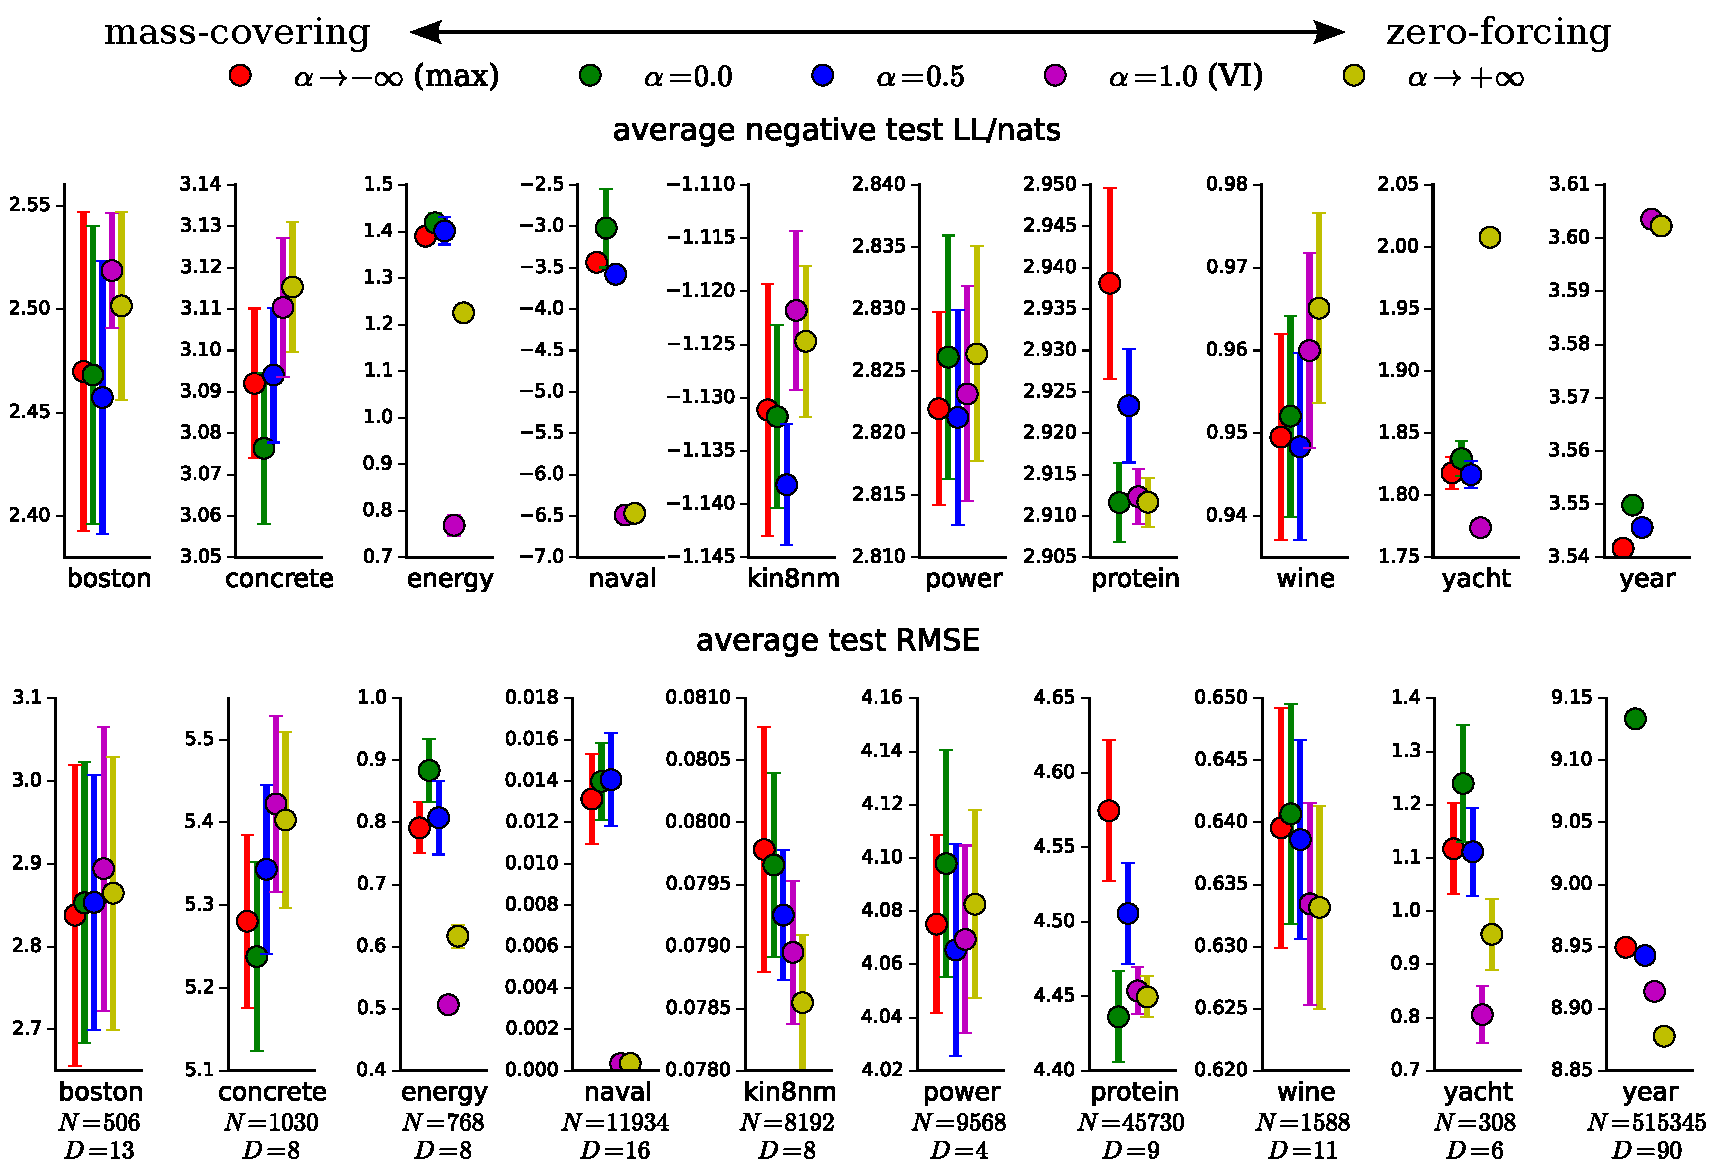
\includegraphics[width=1\linewidth]{Chapter4/vrbound/figs/results_all_bnn}
    \caption{Test LL and RMSE results for Bayesian neural network regression. The lower the better. The error bars show 1-standard deviation across 20 random splits of the data.}
    \label{fig:chap4_vrbound_bnn_results_all}
\end{figure}
%
\begin{figure}
%\begin{table}[ht]
\centering
\captionof{table}{Regression experiment: Average negative test log likelihood/nats}
\label{tab:chap4_vrbound_bnn_ll}
\begin{tabular}{l@{\ica}r@{\ica}r@{\ica}r@{$\pm$}l@{\ica}r@{$\pm$}l@{\ica}r@{$\pm$}l@{\ica}r@{$\pm$}l@{\ica}r@{$\pm$}l@{\ica}}
\hline
\bf{Dataset}&{N}&{D}&\multicolumn{2}{c}{\bf{$\alpha \rightarrow -\infty$}}&\multicolumn{2}{c}{\bf{$\alpha = 0.0$}}&\multicolumn{2}{c}{\bf{$\alpha = 0.5$}}&\multicolumn{2}{c}{\bf{$\alpha = 1.0$ (VI)}}&\multicolumn{2}{c}{\bf{$\alpha \rightarrow +\infty$}}\\
\hline
boston&506&13&2.47&0.08&2.47&0.07&\underline{\textit{2.46}}&\underline{\textit{0.07}}&\textbf{2.52}&\textbf{0.03}&2.50&0.05\\
concrete&1030&8&3.09&0.02&\underline{\textit{3.08}}&\underline{\textit{0.02}}&3.09&0.02&3.11&0.02&\textbf{3.12}&\textbf{0.02}\\
energy&768&8&1.39&0.02&\textbf{1.42}&\textbf{0.02}&1.40&0.03&\underline{\textit{0.77}}&\underline{\textit{0.02}}&1.23&0.01\\
naval&11934&16&-3.43&0.08&\textbf{-3.02}&\textbf{0.48}&-3.58&0.08&\underline{\textit{-6.49}}&\underline{\textit{0.04}}&-6.47&0.09\\
kin8nm&8192&8&-1.13&0.01&-1.13&0.01&\underline{\textit{-1.14}}&\underline{\textit{0.01}}&\textbf{-1.12}&\textbf{0.01}&-1.12&0.01\\
power&9568&4&2.82&0.01&2.83&0.01&\underline{\textit{2.82}}&\underline{\textit{0.01}}&2.82&0.01&\textbf{2.83}&\textbf{0.01}\\
protein&45730&9&\textbf{2.94}&\textbf{0.01}&\underline{\textit{2.91}}&\underline{\textit{0.00}}&2.92&0.01&2.91&0.00&2.91&0.00\\
wine&1588&11&0.95&0.01&0.95&0.01&\underline{\textit{0.95}}&\underline{\textit{0.01}}&0.96&0.01&\textbf{0.97}&\textbf{0.01}\\
yacht&308&6&1.82&0.01&1.83&0.01&1.82&0.01&\underline{\textit{1.77}}&\underline{\textit{0.01}}&\textbf{2.01}&\textbf{0.00}\\
year&515345&90&\underline{\textit{3.54}}&NA&3.55&NA&3.55&NA&\textbf{3.60}&NA&3.60&NA\\
\hline
\multicolumn{3}{c}{\textbf{Average Rank}}&2.80&0.34&3.00&0.45&\textbf{2.20}&\textbf{0.37}&3.20&0.51&3.80&0.39\\
\hline
\end{tabular}
%\end{table}

%\begin{table}[ht]
\centering
\captionof{table}{Regression experiment: Average test RMSE}
\label{tab:chap4_vrbound_bnn_rmse}
\begin{tabular}{l@{\ica}r@{\ica}r@{\ica}r@{$\pm$}l@{\ica}r@{$\pm$}l@{\ica}r@{$\pm$}l@{\ica}r@{$\pm$}l@{\ica}r@{$\pm$}l@{\ica}}
\hline
\bf{Dataset}&{N}&{D}&\multicolumn{2}{c}{\bf{$\alpha \rightarrow -\infty$}}&\multicolumn{2}{c}{\bf{$\alpha = 0.0$}}&\multicolumn{2}{c}{\bf{$\alpha = 0.5$}}&\multicolumn{2}{c}{\bf{$\alpha = 1.0$ (VI)}}&\multicolumn{2}{c}{\bf{$\alpha \rightarrow +\infty$}}\\
\hline
boston&506&13&\underline{\textit{2.84}}&\underline{\textit{0.18}}&2.85&0.17&2.85&0.15&\textbf{2.89}&\textbf{0.17}&2.86&0.17\\
concrete&1030&8&5.28&0.10&\underline{\textit{5.24}}&\underline{\textit{0.11}}&5.34&0.10&\textbf{5.42}&\textbf{0.11}&5.40&0.11\\
energy&768&8&0.79&0.04&\textbf{0.88}&\textbf{0.05}&0.81&0.06&\underline{\textit{0.51}}&\underline{\textit{0.01}}&0.62&0.02\\
naval&11934&16&0.01&0.00&0.01&0.00&\textbf{0.01}&\textbf{0.00}&\underline{\textit{0.00}}&\underline{\textit{0.00}}&0.00&0.00\\
kin8nm&8192&8&\textbf{0.08}&\textbf{0.00}&0.08&0.00&0.08&0.00&0.08&0.00&\underline{\textit{0.08}}&\underline{\textit{0.00}}\\
power&9568&4&4.08&0.03&\textbf{4.10}&\textbf{0.04}&\underline{\textit{4.07}}&\underline{\textit{0.04}}&4.07&0.04&4.08&0.04\\
protein&45730&9&\textbf{4.57}&\textbf{0.05}&\underline{\textit{4.44}}&\underline{\textit{0.03}}&4.51&0.03&4.45&0.02&4.45&0.01\\
wine&1588&11&0.64&0.01&\textbf{0.64}&\textbf{0.01}&0.64&0.01&0.63&0.01&\underline{\textit{0.63}}&\underline{\textit{0.01}}\\
yacht&308&6&1.12&0.09&\textbf{1.24}&\textbf{0.11}&1.11&0.08&\underline{\textit{0.81}}&\underline{\textit{0.05}}&0.96&0.07\\
year&515345&90&8.95&NA&\textbf{9.13}&NA&8.94&NA&8.91&NA&\underline{\textit{8.88}}&NA\\
\hline
\multicolumn{3}{c}{\textbf{Average Rank}}&3.40&0.38&3.70&0.51&3.20&0.31&2.40&0.45&\textbf{2.30}&\textbf{0.38}\\
\hline
\end{tabular}
%\end{table}

       
\end{figure}

We summarise the test negative log-likelihood (LL) and RMSE with standard error (across different random splits except for Year) for selected datasets in Figure \ref{fig:chap4_vrbound_bnn_results_all} and Table \ref{tab:chap4_vrbound_bnn_ll}, \ref{tab:chap4_vrbound_bnn_rmse}. In the tables the best performing results are underlined, while the worse cases are also bold-faced. These results indicate that for posterior approximation problems, the optimal $\alpha$ may vary for different datasets (although for Boston and Power the performances are very similar). 
%

It can be particularly tricky to approximate the posterior distribution of the weight matrices for a neural network. Since one can obtain the same output by swapping the positions of two hidden units and adjusting the corresponding in- and out-going weights, there exist symmetric modes in the exact posterior of the weight matrices. In this case mass-covering can be harmful, e.g.~for Naval and Energy datasets, methods with $\alpha < 1.0$ values seem to be under-performing, not only for predictive error but also for test log-likelihood measure. 
But still, we observed two major trends. Zero-forcing/mode-seeking methods tend to focus on improving the predictive error. Mass-covering methods, on the other hand, returns better test log-likelihood, which has been shown empirically to be correlated with the quality of the approximated uncertainty estimate \citep{hernandez-lobato:pbp2015, gal:uncertainty2016, depeweg:bnn_rl2016}. In particular VI returns lower test log-likelihood for most of the datasets. Furthermore, $\alpha = 0.5$ produced overall good results for both test LL and RMSE, possibly because the skew symmetry is centred at $\alpha = 0.5$ and the corresponding divergence is the only symmetric distance measure in the family. Future work should develop algorithms to automatically select the best $\alpha$ values, although a naive approach could use validation sets. 

\subsection{Variational auto-encoders}

The second experiments considers variational auto-encoders for unsupervised learning. We mainly compare three approaches: VAE ($\alpha = 1.0$), IWAE ($\alpha = 0$), and VR-max ($\alpha = -\infty$), which are implemented upon the publicly available code.\footnote{\url{https://github.com/yburda/iwae}}
%
Four datasets are considered: Frey Face\footnote{\url{http://www.cs.nyu.edu/~roweis/data.html}} (with 10-fold cross validation), Caltech 101 Silhouettes\footnote{\url{https://people.cs.umass.edu/~marlin/data.shtml}}, MNIST\footnote{\url{http://yann.lecun.com/exdb/mnist/}} and OMNIGLOT\footnote{\url{https://github.com/brendenlake/omniglot}}. The VAE model has $L=1, 2$ stochastic layers with deterministic layers stacked between.  The detailed numbers of stochastic layers $L$, number of hidden units, and the activation function are summarised in Table \ref{tab:vae_arch}. The prefix of the number indicates whether this layer is \textbf{d}eterministic or \textbf{s}tochastic, e.g.~d500-s200 stands for a neural network with one deterministic layer of 500 units followed by a stochastic layer of 200 units. For Frey Face data we train the models using learning rate 0.0005 and mini-batch size 100. For MNIST and OMNIGLOT we reuse the settings from \cite{burda:iwae2016}: the training process runs for $3^i$ passes with learning rate $0.0001 \cdot 10^{-i/7}$ for $i = 0, ..., 7$, and the batch size is 20. For Caltech Silhouettes we use the same settings as MNIST and OMNIGLOT except that the training proceeded for $\sum_{i=0}^7 2^i = 255$ epochs. We reproduce the IWAE experiments to obtain a fair comparison, since the results in the original publication \citep{burda:iwae2016} mismatches those evaluated on the publicly available code.
%

\begin{table}[!ht]
\centering
\captionof{table}{Network architecture of tested VAE algorithms.}
\label{tab:vae_arch}
\begin{tabular}{lccccc}
\hline
\bf{Dataset}&$L$&architecture&activation&probability type (p/q)\\
\hline
Frey Face&1& d200-d200-s20&softplus&Gaussian/Gaussian\\
\hline
Caltech 101& 1&d500-s200&tanh&Bernoulli/Gaussian\\
\hline
MNIST \& & 1&d200-d200-s50&tanh&Bernoulli/Gaussian\\
OMNIGLOT     & 2&d200-d200-s100-d100-d100-s50&tanh&Bernoulli/Gaussian\\
\hline
\end{tabular}
\end{table}

%

\begin{figure}
\begin{minipage}{0.6\linewidth}

%\begin{table}[t]
\centering
%\caption
\captionof{table}{ Average Test log-likelihood. Results for VAE on MNIST and OMNIGLOT are collected from \cite{burda:iwae2016}.}
\label{tab:vae_ll}
\begin{tabular}{lccccc}
\toprule
\bf{Dataset}&$L$&$K$&\bf{ VAE }&\bf{ IWAE }&\bf{ VR-max }\\
\hline
Frey Face&1&5&1322.96&\bf{1380.30}&1377.40\\
($\pm$ std. err.)& & &$\pm$10.03&\bf{$\pm$4.60}&$\pm$4.59 \\
\hline
Caltech 101& 1& 5&-119.69&\bf{-117.89}&-118.01\\
Silhouettes&  &50&-119.61&-117.21&\bf{-117.10}\\
\hline
MNIST& 1&5 &-86.47&\bf{-85.41}&-85.42\\
     &  &50&-86.35&\bf{-84.80}&-84.81\\
     & 2&5 &-85.01&\bf{-83.92}&-84.04\\
     &  &50&-84.78&\bf{-83.05}&-83.44\\
\hline
OMNIGLOT & 1&5 &-107.62&\bf{-106.30}&-106.33\\
		 & 1&50&-107.80&\bf{-104.68}&-105.05\\
		 & 2&5 &-106.31&\bf{-104.64}&-104.71\\
		 & 2&50&-106.30&\bf{-103.25}&-103.72\\
\bottomrule
\end{tabular}
%\end{table}

\end{minipage}
\hfill
\begin{minipage}{0.35\linewidth}
\centering
 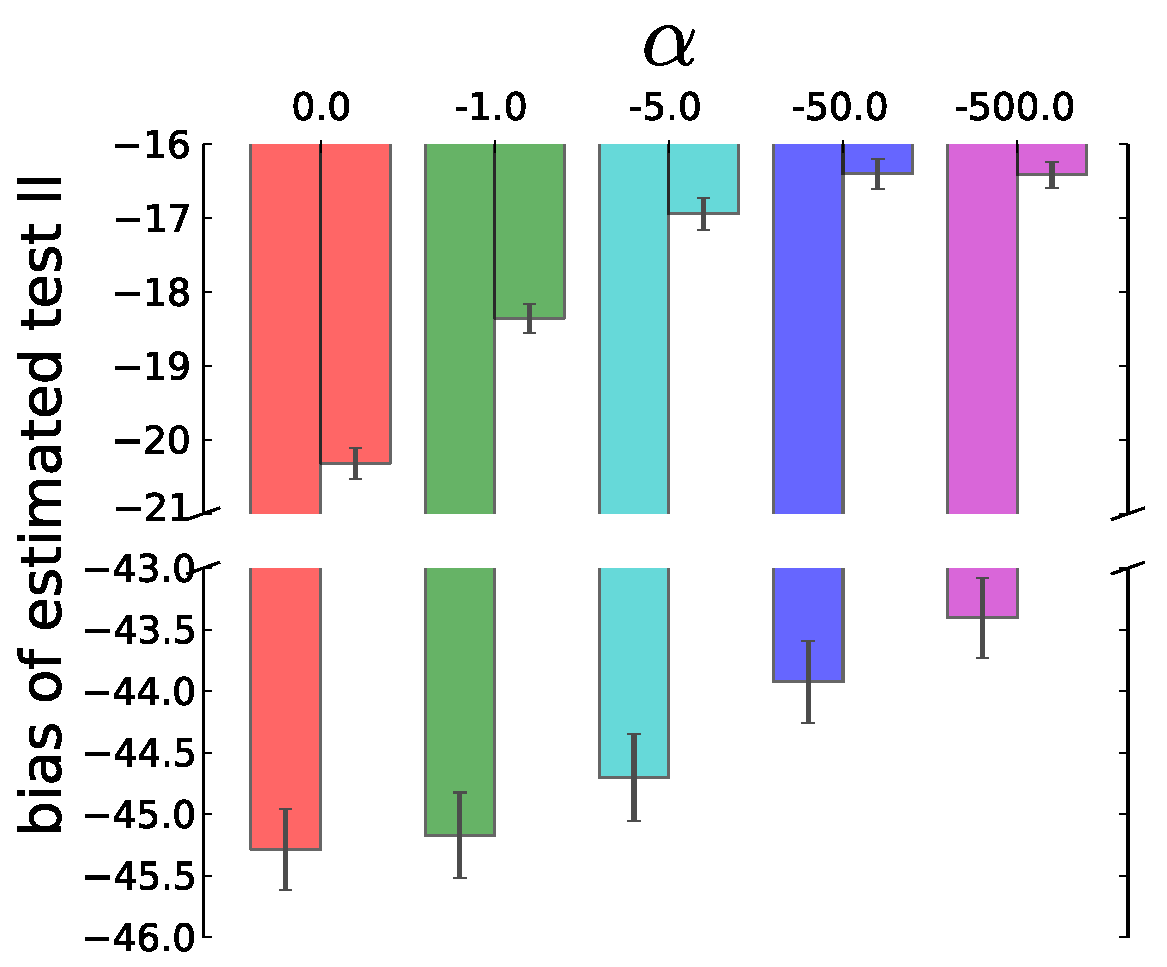
\includegraphics[width=1.00\linewidth]{Chapter4/vrbound/figs/bias_estimate.pdf} 
 \captionof{figure}{Bias of sampling approximation to. Results for $K=5, 50$ samples are shown on the left and right, respectively.}
 \label{fig:vae_bias}
\end{minipage}
\end{figure}
%
\begin{figure*}[!ht]
 \centering
 \subfigure[Log of ratio $R = w_{max} / (1 - w_{max})$]{
 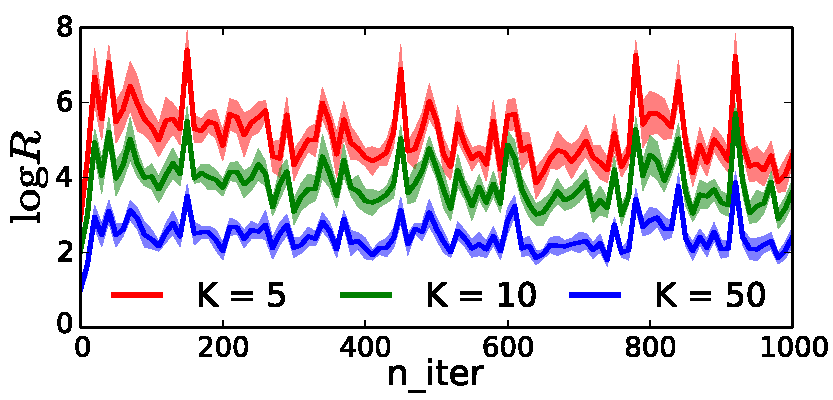
\includegraphics[width=0.37\linewidth]{Chapter4/vrbound/figs/weight_ratio.pdf}
 \label{fig:weight_ratio}}
 \hspace{0.4in}
 \subfigure[Weights of samples.]{
 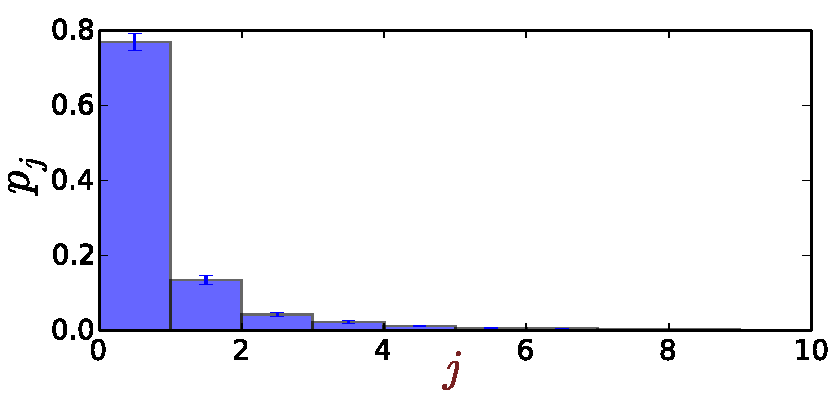
\includegraphics[width=0.37\linewidth]{Chapter4/vrbound/figs/weight_distribution.pdf}
 \label{fig:weight_distribution}}
 \caption{Importance weights during training, see main text for details. Best viewed in colour.}
\end{figure*}

We report test log-likelihood results in Table \ref{tab:vae_ll} by computing $\log p(\bm{x}) \approx \hat{\mathcal{L}}_{0, 5000}(q; \bm{x})$ following \cite{burda:iwae2016}. We also present some samples from the VR-max trained auto-encoders in Figure \ref{fig:vae_samples}.
%
\begin{figure}
 \centering
  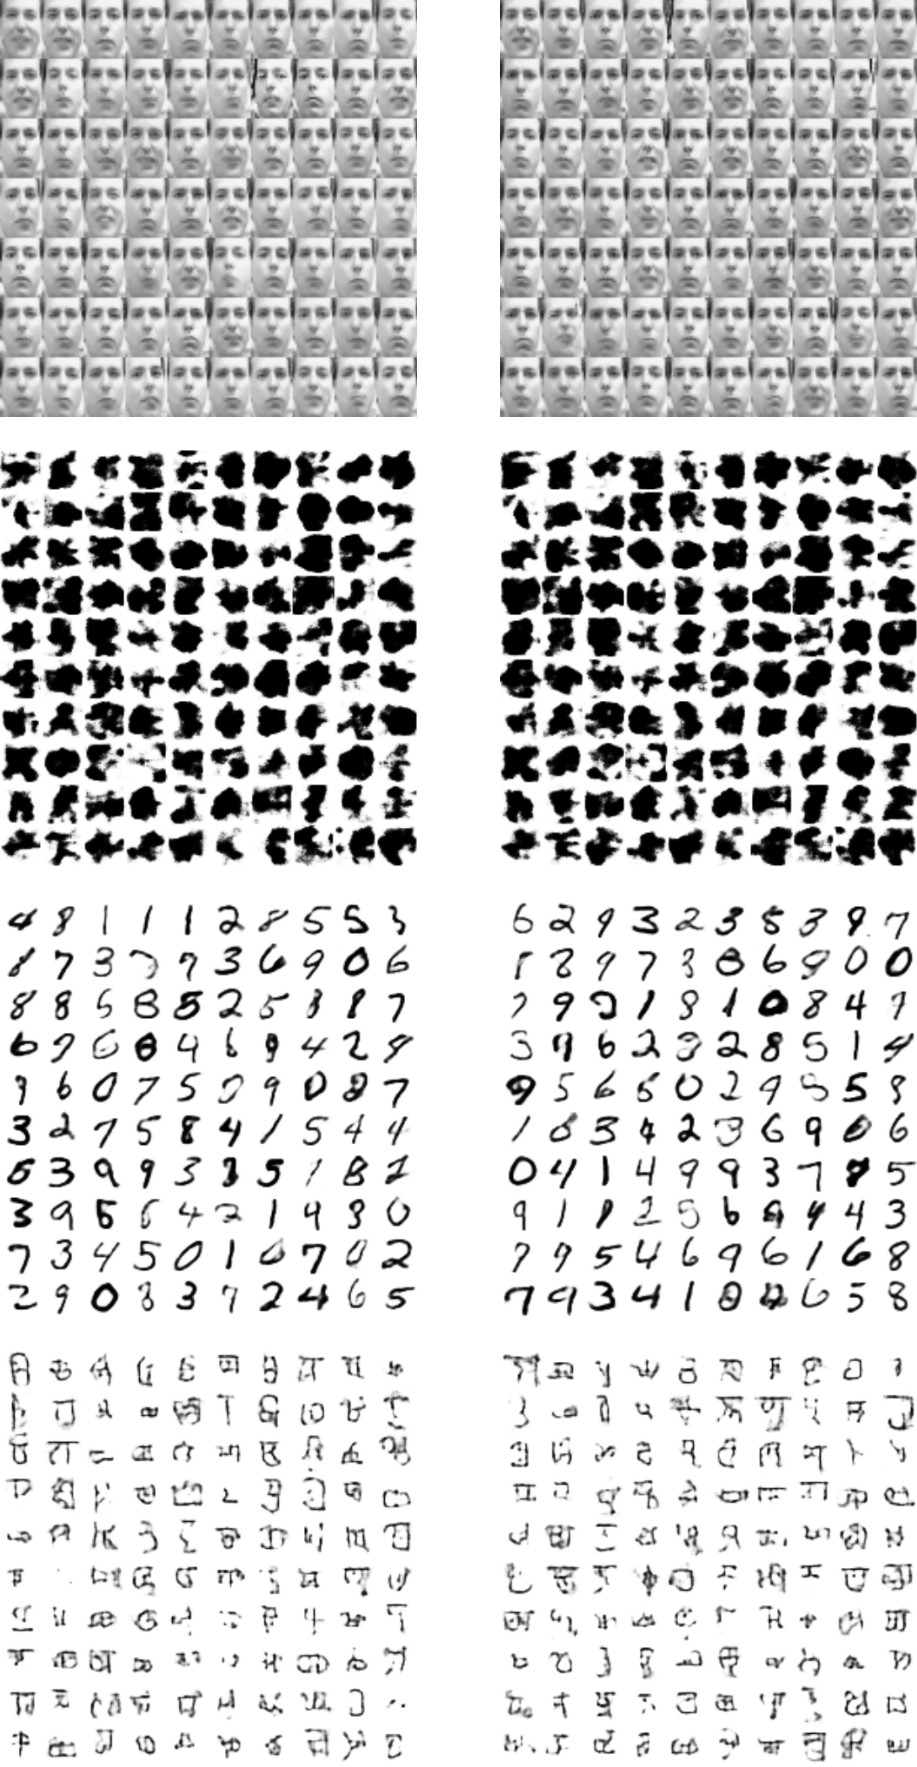
\includegraphics[width=0.6\linewidth]{Chapter4/vrbound/figs/vae_samples.pdf}
  \caption{Sampled images from the the best models trained with IWAE (left) and VR-max (right).}
  \label{fig:vae_samples}
\end{figure}
%
Overall VR-max is almost indistinguishable from IWAE. Other positive alpha settings (e.g.~$\alpha = 0.5$) return worse results, e.g. $1374.64\pm5.62$ for Frey Face and $-85.50$ for MNIST with $\alpha = 0.5$, $L=1$ and $K=5$. These worse results for $\alpha > 0$ indicate the preference of getting tighter approximations to the likelihood function for MLE problems. Small negative $\alpha$ values (e.g.~$\alpha = -1.0, -2.0$) return better results on different splits of the Frey Face data, and overall the best $\alpha$ value is dataset-specific.\footnote{Since presentation of this work at NIPS 2016, \cite{bui:dgm2016} revisited this idea with slightly different architecture set-up, and showed that $\alpha \neq 0$ values are usually favoured over the IWAE approach. }

VR-max's success might be explained by the tightness of the bound. To evaluate this, we compute the VR bounds on $100$ test datapoints using the 1-layer VAE trained on Frey Face, with $K=\{5, 50\}$ and $\alpha \in \{0, -1, -5, -50, -500 \}$. Figure \ref{fig:vae_bias} presents the estimated gap $\hat{\mathcal{L}}_{\alpha, K} - \hat{\mathcal{L}}_{0, 5000}$. The results indicates that $\hat{\mathcal{L}}_{\alpha, K}$ provides a lower-bound, agreeing with the theoretical results presented in Section \ref{sec:chap4_vrbound_sampling}, and that gap is narrowed as $\alpha \rightarrow -\infty$. Also increasing $K$ provides improvements. The standard error of estimation is almost constant for different $\alpha$ (with $K$ fixed), and is negligible when compared to the MC approximation bias.

%
Another explanation for VR-max's success is that, the sample with the largest normalised importance weight $w_{max}$ dominates the contributions of all the gradients.
This is confirmed by tracking $R = \frac{w_{max}}{1 - w_{max}}$ during training on Frey Face (Figure \ref{fig:weight_ratio}). Also Figure \ref{fig:weight_distribution} shows the $10$ largest importance weights from $K=50$ samples in descending order, which exhibit an exponential decay behaviour, with the largest weight occupying more than $75\%$ of the probability mass. This means, the IWAE algorithm is not efficient in terms of sample efficiency, since the learning signal from back-propagation is dominated by the gradients computed on the particle with the largest weight.
%
It also indicates that, VR-max can provide a fast approximation to IWAE when tested on CPUs or multiple GPUs with high communication costs. Indeed our numpy implementation of VR-max achieves up to a 3 times speed-up compared to IWAE (9.7s vs.~29.0s per epoch, tested on Frey Face data with $K = 50$ and batch size $M = 100$, CPU info: Intel Core i7-4930K CPU @ 3.40GHz). However this speed advantage is less significant when the gradients can be computed very efficiently on a single GPU.
\section{Summary}
We have introduced the variational R{\'e}nyi bound and an associated optimisation framework. We have shown the richness of the new family, not only by connecting to existing approaches including VI/VB, SEP, BB-$\alpha$, VAE and IWAE, but also by proposing the VR-max algorithm as a new special case. Empirical results on Bayesian neural networks and variational auto-encoders indicate that VR bound methods are widely applicable and can obtain state-of-the-art results.
%
%
Future work will focus on both experimental and theoretical aspects. Theoretical work will study the interaction of the biases introduced by MC approximation and datapoint sub-sampling. Also a quantitative analysis of the MC approximation bias will be very useful, especially for model selection. 

%\section{Free-energy construction with decoupling and constraint relaxations}
%\label{sec:constraint_relaxation_all}
%\subsection{EP energy: a primal-dual story}
\label{sec:chap2_ep_energy}

EP has been criticised for not having convergence guarantees and instead being a heuristic for posterior approximation. On the other hand, it has been shown to have superior performance compared to VI on a variety of tasks, e.g.~Gaussian Process classification \citep{kuss:gpep2005}. To understand these seemingly contradicting observations, here we provide an energy minimisation view of EP,\footnote{material based on my NIPS 2016 approximate inference workshop abstract, see publication page.} and discuss why EP could potentially lead to better approximations, and why it is difficult to prove the convergence of EP. Similar derivations are also available in \citet{yedidia:bethe2001, heskes:ep2002, minka:divergence2005, opper:ec2005, wainwright:graphical2008}, and some extensions to handling latent variable models are provided in appendix \ref{sec:appendix_relaxation}.

To streamline the notation, we consider approximating the intractable posterior $p(\mparam|\mathcal{D}) = \frac{1}{Z} p_0(\mparam) \prod_{n=1}^N p(\bm{x}_n|\mparam)$ as a running example. In this case we denote $\tilde{f}_n(\mparam) = p(\bm{x}_n|\mparam)$ and leave the prior $p_0(\mparam)$ as it is. Using this notation we again write down the objective function of Variational inference (VI) called the \emph{variational free energy} (VFE) \citep{jordan:vi1999, beal:vi2003}:
\begin{equation}
\min_{q \in \mathcal{Q}} \mathrm{KL}[q||p] \Leftrightarrow \min_{q \in \mathcal{Q}} \mathcal{F}_{\text{VFE}}(q) = \mathbb{E}_{q} \left[ \log q(\mparam) - \log p_0(\mparam) - \sum_{n=1}^N \log \tilde{f}_n(\mparam) \right].
\label{eq:ep_section_vfe}
\end{equation}

\subsubsection{From VFE to Bethe Free Energy}
\label{sec:vfe_to_bethe}

First we make use of the additivity of logarithm to rewrite an equivalent optimisation problem (recall that $\mathcal{P}$ is the space of all probability distributions):
\begin{equation}
\begin{aligned}
\min_{q \in \mathcal{Q}} \mathcal{F}_{\text{VFE}}(q)
&= \min_{q \in \mathcal{Q}} \mathrm{KL}[q||p_0] - \sum_n \mathbb{E}_{q} \left[ \log \frac{p_0(\mparam) \tilde{f}_n(\mparam)}{q(\mparam)} \right] - N \mathrm{KL}[q || p_0] \\
& = \min_{ q \in \mathcal{Q}, \{ \tilde{p}_n \in \mathcal{P} \} } (1 - N) \mathrm{KL}[q||p_0] - \sum_n \mathbb{E}_{\tilde{p}_n} \left[ \log \frac{p_0(\mparam) \tilde{f}_n(\mparam)}{\tilde{p}_n(\mparam)} \right] \\ 
& \quad \quad \quad \quad \text{ subject to } \tilde{p}_n = q, \forall n. 
\end{aligned}
\label{eq:vi_constrained}
\end{equation}
%
Here in the first line we added $N$ copies of $\mathrm{KL}[q || p_0]$ to the VFE and subtracted the same, and in the second line we \emph{decoupled} the tilted distribution $\tilde{p}_n$ from $q$ by introducing equality constraints. This means the above optimisation has the same fixed points as minimising VFE. The constraints can be \emph{relaxed} to matching all the moments $\mathbb{E}_{\tilde{p}_n}[\mparam^{k}] = \mathbb{E}_q[\mparam^k]$ for $k \in \mathbb{N}$,\footnote{Having the same moments for $p$ and $q$ does not imply having the same \emph{moment generating function}.} and a further crude relaxation suggests moment matching just for the first $K$ moments\footnote{The zeroth moment matching constraint is replaced by the constraint that $\tilde{p}_n$ integrates to 1.}
$\mathbb{E}_{\tilde{p}_n}[\mparam^{k}] = \mathbb{E}_q[\mparam^k], k = 1, 2, ..., K$.
%
In the following we use a vectorial function $\bm{\Phi}(\mparam)$ to summarise these constraints as $\mathbb{E}_{\tilde{p}_n}[\bm{\Phi}] = \mathbb{E}_q[\bm{\Phi}]$, where as an example for Gaussian EP: $\bm{\Phi}(\mparam) = [\mparam, \mparam \mparam^T]$. In general $\bm{\Phi}$ can contain any polynomial terms or other basis functions. This relaxation returns the following constrained optimisation problem:
%
\begin{equation}
\begin{aligned}
 \min_{ q \in \mathcal{Q}, \{ \tilde{p}_n \in \mathcal{P} \} } \mathcal{F}_{\text{Bethe}}( \{ \tilde{p}_n \}, q) \quad \text{subject to } \mathbb{E}_{\tilde{p}_n}[\bm{\Phi}] = \mathbb{E}_q[\bm{\Phi}], \forall n, \\
\mathcal{F}_{\text{Bethe}}( \{ \tilde{p}_n \}, q) =  (1 - N) \mathrm{KL}[q||p_0] - \sum_n \mathbb{E}_{\tilde{p}_n} \left[ \log \frac{p_0(\mparam) \tilde{f}_n(\mparam)}{\tilde{p}_n(\mparam)} \right].
\end{aligned}
\label{eq:bethe}
\end{equation}
$\mathcal{F}_{\text{Bethe}}( \{ \tilde{p}_n \}, q)$ is the \emph{Bethe free energy} \citep{bethe:energy1935, yedidia:bethe2001} that is usually presented in the context of probabilistic graphical models and belief propagation. Below we show how to derive its dual form that is usually discussed in EP literature \citep{minka:ep_energy2001, opper:ec2005, seeger:ep2005}. 

\vspace{1em}
\begin{tcolorbox}
\textbf{Remark} (Tom Minka's original note)\textbf{.}
\cite{minka:ep_energy2001} formulated (\ref{eq:bethe}) as a minimax problem ($\min_{\{\tilde{p}_n \}} \max_{q}$) instead which seems questionable to me.  First (\ref{eq:bethe}) relaxes the constraints in (\ref{eq:vi_constrained}), meaning both should have the same optimisation direction. Then since (\ref{eq:vi_constrained}) just decouples VFE (\ref{eq:ep_section_vfe}) with equality constraints, it should be a pure minimisation and has the same stationary points. For graphical models the Bethe free energy optimisation problem is formulated as a pure minimisation problem like above (\ref{eq:bethe}), e.g.~in \cite{heskes:bp_fixed_point2002, wainwright:graphical2008} but also interestingly in pages 3-4 of \cite{minka:ep_energy2001}. On the other hand, Minka's derivation of the dual energy differs from solving the Lagrangian and does not require the minimax assumption of the primal problem. 
\end{tcolorbox}

\subsubsection{From Bethe to EP: a dual form representation}
\label{sec:ep_fixed_points}
We provide a derivation in a similar way as \cite{heskes:bp_fixed_point2002}, starting from a note on the KL duality\footnote{We include this step in order to connect to the EP energy with optimisation arguments all in the dual space.}
\begin{equation}
 -\mathrm{KL}[q||p_0] = \min_{\bm{\lambda}_{q}(\mparam)} - \mathbb{E}_q[\lambda_q(\mparam)] + \log \mathbb{E}_{p_0} \left[ \exp [\lambda_q(\mparam)] \right],
 \label{eq:kl_duality}
\end{equation}
with $\lambda_q(\mparam)$ a function to be specified later on. This duality is in the same spirit as deriving convex conjugate function for the log partition function of an exponential family distribution (see Proposition \ref{prop:chap2_expfam}), if viewing $p_0(\mparam)$ as the base measure.
The equality is achieved by $q(\mparam) \propto p_0(\mparam) \exp[\lambda_q(\mparam)]$.
%
Substitution into (\ref{eq:bethe}) then yields a transformed energy that we denoted as $\mathcal{F}_{\text{Bethe}}(\{ \tilde{p}_n \}, q, \lambda_q(\mparam))$.
%
\begin{equation}
\begin{aligned}
\mathcal{F}_{\text{Bethe}}(\{ \tilde{p}_n \}, q, \lambda_q(\bm{\theta})) = (1 - N) \mathbb{E}_q[\lambda_q(\bm{\theta})] + (N - 1) \log \mathbb{E}_{p_0} \left[ \exp [\lambda_q(\bm{\theta})] \right] \\
- \sum_n \mathbb{E}_{\tilde{p}_n} \left[ \log \frac{p_0(\bm{\theta}) \tilde{f}_n(\bm{\theta})}{\tilde{p}_n(\bm{\theta})} \right].
\label{eq:bethe_energy_transformed}
\end{aligned}
\end{equation}

%
Denote $\bm{\lambda}_{-n}$ as the Lagrange multiplier for moment matching and $\nu, \nu_n$ for the normalisation constraints of $q$ and $\tilde{p}_n$, respectively. This returns the following Lagrangian
\begin{equation}
\begin{aligned}
 \min_{q, \{ \tilde{p}_n \}, \lambda_q(\bm{\theta}) } \max_{\{ \bm{\lambda}_{-n}, \nu_n, \nu \} } \mathcal{F}_{\text{Bethe}}( \{ \tilde{p}_n \}, q, \lambda_q(\bm{\theta})) + \sum_n \bm{\lambda}_{-n}^{T}(\mathbb{E}_q[\bm{\phi}] - \mathbb{E}_{\tilde{p}_n}[\bm{\phi}]) \\
 + \sum_n \nu_n \left( \int \tilde{p}_n(\bm{\theta}) d\bm{\theta} - 1 \right) + \nu \left( \int q(\bm{\theta}) d\bm{\theta} - 1 \right) .
\end{aligned} 
\label{eq:bethe_lagranrian}
\end{equation}
Solving the fixed points for $\tilde{p}_n$ and $\nu_n$ returns 
$$
\tilde{p}_n(\mparam) = \frac{1}{Z_n} p_0(\mparam)\tilde{f}_n(\mparam) \exp \left[ \bm{\lambda}_{-n}^T \bm{\Phi}(\mparam) \right],
$$
where the normalising constant is $$Z_n = \int p_0(\mparam) \tilde{f}_n(\mparam) \exp \left[ \bm{\lambda}_{-n}^T \bm{\Phi}(\mparam) \right] d \mparam.$$ 
%
Also it is straight-forward to evaluate the fixed point condition for $q$: $$(N - 1) \lambda_q(\mparam) = \sum_n \bm{\lambda}_{-n}^T \bm{\Phi}(\mparam) + \nu.$$
We explicitly specify $\lambda_q(\mparam) = \bm{\lambda}_q^T \bm{\Phi}(\mparam) + \nu$ w.l.o.g., also the constant $\nu$ can be dropped since exponential family distributions are translation invariant to constants.
%
Importantly, substituting $\tilde{p}_n$ back to (\ref{eq:bethe_lagranrian}) and enforcing the fixed point condition for $q$ yields the \emph{EP energy} \citep{minka:ep_energy2001}:
\begin{equation}
\begin{aligned}
\min_{\bm{\lambda}_q} \max_{\{ \bm{\lambda}_{-n} \} } \mathcal{F}_{\text{EP}}(\bm{\lambda}_q, \{ \bm{\lambda}_{-n} \} ) =  (N - 1) \log \mathbb{E}_{p_0} \left[ \exp [\bm{\lambda}_q^T \bm{\Phi}(\mparam)] \right] - \sum_n \log Z_n,\\
 \text{subject to } (N - 1) \bm{\lambda}_q = \sum_n \bm{\lambda}_{-n}.
\end{aligned}
\label{eq:ep_energy}
\end{equation}
Notice now the optimisation problem over $q$ is dropped since (\ref{eq:ep_energy}) does not depend on it. To obtain the approximate posterior back, we make use of the tightness of the KL duality, and define 
$$q(\mparam) = \frac{1}{Z_q} p_0(\mparam) \exp \left[ \bm{\lambda}_q^T \bm{\Phi}(\mparam) \right],  \quad \log Z_q = \log \mathbb{E}_{p_0} \left[ \exp [\bm{\lambda}_q^T \bm{\Phi}(\mparam)] \right].$$
%
The expectation consistent approximate inference (EC) algorithm \citep{opper:ec2005} is a special case with $p_0(\mparam) \propto 1$ and $N = 2$. 

\subsubsection{EP as a fix point iteration method for solving the dual problem}

EP \citep{minka:ep2001} proposes parametrising the (natural parameters of) local approximating factors $f_n \approx \tilde{f}_n$ instead of the approximate posterior $q$, with the goal of $f_n$ capturing the effect of $\tilde{f}_n(\mparam)$ on the exact posterior, by defining $f_n(\mparam) = \exp [\bm{\lambda}_n^T \bm{\Phi}(\mparam)]$, $\bm{\lambda}_n = \bm{\lambda}_q - \bm{\lambda}_{-n}$. Thus by construction the constraint in (\ref{eq:ep_energy}) is automatically satisfied: $\bm{\lambda}_q = \sum_n \bm{\lambda}_n$ and $\bm{\lambda}_{-n} = \sum_{m \neq n} \bm{\lambda}_m$.
%
Then EP runs a fixed point iteration algorithm to find a stationary point for $\{ \bm{\lambda}_n \}_{n=1}^N$. More specifically the gradient of (\ref{eq:ep_energy}) w.r.t.~the local parameter $\bm{\lambda}_n$ is 
\begin{equation}
\nabla_{\bm{\lambda}_n} \mathcal{F}_{\text{EP}} = (N-1) \mathbb{E}_{q} [ \bm{\Phi}(\mparam) ] - \sum_{m \neq n} \mathbb{E}_{\tilde{p}_m} [ \bm{\Phi}(\mparam) ].
\end{equation} 
Zeroing the above gradient for all $\bm{\lambda}_n$ results in the fixed point condition
$$\mathbb{E}_q[\bm{\Phi}(\mparam)] = \mathbb{E}_{\tilde{p}_n}[ \bm{\Phi}(\mparam) ], \quad \forall n,$$
which motivates the moment matching update (\ref{eq:chap2_ep_moment_matching}) in EP.

\subsubsection{A pictorial view on why EP can be better than VI}
Folk wisdom suggests that EP, if it convergences, often provide more accurate approximations to the target distribution when compared with VI. This observation is explained pictorially in Figure \ref{fig:chap2_ep_vi_comparison}. 
%
Recall that both algorithms can be viewed as minimising the Bethe free energy under constraints: for VI the constraints are equality constraints $q = \tilde{p}_n$, whereas EP instead uses moment matching constraints $\mathbb{E}_q[\bm{\Phi}] = \mathbb{E}_{\tilde{p}_n}[\bm{\Phi}]$. In an augmented space $\mathcal{P}^{N+1}$, the search space of VI $\{ (q, \tilde{p}_n): q = \tilde{p}_n, q \in \mathcal{Q} \}$ is contained in the search space of EP $ \{ (q, \tilde{p}_1, ..., \tilde{p}_N): q \in \mathcal{Q}, \mathbb{E}_{\tilde{p}_n}[\bm{\Phi}] = \mathbb{E}_q[\bm{\Phi}] \}$, and can be of much smaller dimensions (e.g.~the green line segment versus the blue region as shown in the Figure \ref{fig:chap2_ep_vi_comparison}). Therefore if EP converges, then it is more likely to find a better minimum compared to VI. Empirical evidence also suggests that constrained Bethe free-energy evaluated at a fixed point is often a better approximation to the (negative log) marginal likelihood.

\begin{figure}
\centering
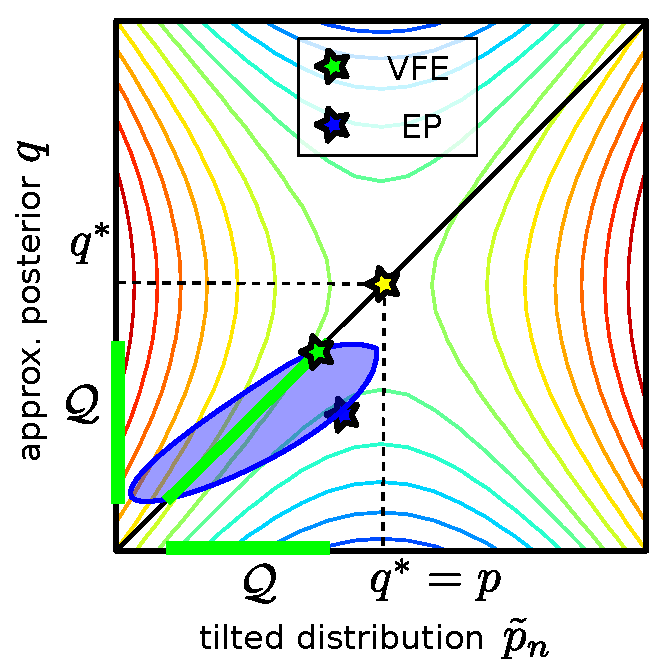
\includegraphics[width=0.4\linewidth]{Chapter2/ep/energy.pdf}
\caption{EP versus VI as constrained energy optimisation problems, visualised by projecting the energy surface from the augmented space $\mathcal{P}^{N+1}$ to $\mathcal{P}^{2}$. Here the slash line across the space represents the subspace $\{ (q, \tilde{p}_n): q = \tilde{p}_n \}$, and the search space for VI (the green segment) is contained in the EP candidate set (the blue region). The stars indicate the optimal solutions returned by the exact (in yellow) and the approximate inference algorithms (green/blue). See main text for details.}
\label{fig:chap2_ep_vi_comparison}
\end{figure}

\subsubsection{Criticisms for EP's iterative update}
%
The above fixed point iteration update has no convergence guarantee, which is one of the drawbacks of EP. The reason is that EP solves the dual problem of constrained Bethe free energy minimisation, and that dual problem turns out to be a minimax optimisation problem with constraints. Indeed, a double-loop algorithm \citep{heskes:ep2002} should be applied to (\ref{eq:ep_energy}) if convergence is required. However in practice such a double-loop method has been shown to be much slower than EP. Also disappointedly, even when the exact posterior is contained in $\mathcal{Q}$, EP is not guaranteed to return it. Similar problems exist for belief propagation when the graph contains many loops, or when the relaxed polytope is not \emph{tight} \citep{wainwright:graphical2008}.

%\hl{Another myth about EP is the choice of using fixed point update instead of gradient descent for the local parameters. Here it should be emphasised that the optimisation aims to find a \emph{saddle point} rather than a local minimum/maximum of the energy function. Since it is a minimisation problem for $\bm{\lambda}_q$ and maximisation problem for $\bm{\lambda}_{-n}$, is is also unclear to determine the optimisation problem for the local parameters $\bm{\lambda}_n$. Finally there exists no proof that the EP energy is upper or lower bounded, i.e. the existence of minimum/maximum is unclear as well. All the above situations make the analysis of gradient descent convergence very difficult.}


\subsubsection{From VFE to power EP}
\label{sec:vfe_to_pep}
We now extend the above approach to power EP \citep{minka:powerep2004} which is a new contribution, although fairly straightforward. This procedure includes one modification to the Bethe free energy. Assume for each factor $\tilde{f}_n$ a power value $\alpha_n \neq 0$ is associated, with $\bm{\alpha} = (\alpha_1, ..., \alpha_N)$ and $\sum_n \frac{1}{\alpha_n} \neq 1$. Then the Bethe free energy with moment matching constraints is modified to:
\begin{equation}
\mathcal{F}_{\bm{\alpha}}(q, \{ \tilde{p}_n \}) = \left( 1 - \sum_n \frac{1}{\alpha_n} \right) \mathrm{KL}[q||p_0] - \sum_{n=1}^N \frac{1}{\alpha_n} \mathbb{E}_{\tilde{p}_n} \left[ \log \frac{p_0(\mparam) \tilde{f}_n(\mparam)^{\alpha_n}}{\tilde{p}_n(\mparam)} \right].
\label{eq:alpha_bethe}
\end{equation}
%
Similar to the derivation of (\ref{eq:vi_constrained}), here we first added and subtracted $(\sum_n \frac{1}{\alpha_n})$ copies of $\mathrm{KL}[q||p_0]$, then decoupled $\tilde{p}_n$ from $q$, and relaxed the equality constraints to moment matching. Calculations following Section \ref{sec:ep_fixed_points} also reveal the change of the fixed point condition for $q$ to $(\sum_n \frac{1}{\alpha_n} - 1) \bm{\lambda}_q = \sum_n \frac{1}{\alpha_n} \bm{\lambda}_{-n}$. Define $q$ as an exponential family distribution with natural parameter $\bm{\lambda}_q$ as before, and $\bm{\lambda}_n = (\bm{\lambda}_q - \bm{\lambda}_{-n}) / \alpha_n$. We arrive at the power EP objective:
\begin{equation}
\left( \sum_n \frac{1}{\alpha_n} - 1 \right) \log Z_q - \sum_n \frac{1}{\alpha_n} \log \int p_0(\mparam) \tilde{f}_n(\mparam)^{\alpha_n} \exp \left[ (\bm{\lambda}_q - \alpha_n \bm{\lambda}_n)^T \bm{\Phi}(\mparam) \right] d \mparam.
\label{eq:pep_energy}
\end{equation}
The iterative process also enforces $\bm{\lambda}_q = \sum_n \bm{\lambda}_n$.  \cite{minka:divergence2005} showed that (\ref{eq:pep_energy}) becomes an upper-bound of $\log Z$ when $\alpha_n > 0$ and $\sum_n \frac{1}{\alpha_n} < 1$. On the other hand, taking $\alpha_n \rightarrow 0, \forall n$ recovers $\mathcal{F}_{\text{VFE}}$ but now the $q$ distribution is restricted to have an exponential family form.
%\input{Chapter4/constraint/bbalpha}
%\input{Chapter4/constraint/distributed}
%\input{Chapter4/constraint/lvm}
%\input{Chapter4/constraint/sequential}
%
%\section{Derivations and proofs}
%\label{sec:proofs_chap4}
%\input{Chapter4/proofs/details_vrbound}

\vspace{3em}
{\Large
\noindent \hrulefill \hspace{0.2cm} \raisebox{-4pt}[10pt][10pt]{\decofourleft ~  \decosix ~ \decofourright} \hspace{0.1cm} \hrulefill
\vspace{2em}
}

This ends the first part of the thesis, which has reviewed existing variational methods (Chapter \ref{chap:background}), and proposed two unifying frameworks for both algorithmic (Chapter \ref{chap:factor_tying}) and optimisation objective (Chapter \ref{chap:vrbound}) aspects. Experiments on Bayesian deep learning tasks also proved the successfulness of our efforts, on pushing variational algorithms towards wider applicability (far beyond conjugate models) and better scalability to ``big data, big models''. I do admit that, however, the lack of theoretically rigorous selection of approximate inference algorithms is one of the imperfections of the analysis presented here. 
%
Indeed, a guide on choosing the optimal inference method are needed for practitioners when applying the framework to their applications, which will be one of my research directions in the future.

So far we only studied different optimisation procedures assuming a given approximating distribution family (mean-field Gaussians in the empirical results), which is just one side of the story for approximate inference. The whole picture for this huge subject will never be comprehensive without discussing the other side, i.e.~the construction of $q$ distributions. In the second part of the thesis ``wild approximate inference'', I will revisit the fundamental questions in approximate inference, providing my point of view on the principles of approximate distribution design, and present one of the algorithms I developed during my PhD following these principles.



\part{Wild Approximate Inference}
\chapter{Wild Approximate Inference: Why and How}
\label{chap:wild}

% **************************** Define Graphics Path **************************
\ifpdf
    \graphicspath{{Chapter5/figs/Raster/}{Chapter5/figs/PDF/}{Chapter5/figs/}}
\else
    \graphicspath{{Chapter5/figs/Vector/}{Chapter5/figs/}}
\fi

The design of approximating distributions is equally, if not more, crucial to the invention of optimisation algorithms such as the two algorithms presented in previous chapters. Mean-field approximations are often ineffective! Apparently if the $\mathcal{Q}$ family is expressive enough to contain the exact posterior, variational inference, either with KL divergence or R{\'e}nyi divergence, would return it as the only global optimum. Hence if a more complex structure is included in the q distribution, the approximation might become much more accurate and potentially even exact. For this purpose, it would be useful to use universal functional approximators, e.g.~neural networks, to expand the distribution family of approximations. However, it becomes very challenging to use these flexible approximations due to many restrictions, which cannot be addressed by simply investing more computational resources (say more running time and memory). 

In recent years, one major research direction is to go beyond mean-field methods via development of flexible $q$ distributions, which specifically addresses the intractability issues when applied to VI. For example, invertible transformations are utilised to construct $q$ distributions which allow analytical evaluations of the approximate posterior density \citep{rezende:flow2015, kingma:iaf2016, louizos:multiplicative2017}. Mixture distributions of more flexible forms are also introduced to capture the possible multi-modality of the exact posterior, with further approximations being proposed to account for extra computational challenges \citep{salimans:mcmcvi2015, tran:vgp2016, ranganath:hvm2016,maaloe:agdm2016}. Though effective, these methods are complicated for practitioners to understand, let alone the design work itself that requires lots of care.

In the second theme of the thesis, an alternative research direction will be presented towards using flexible approximations in approximate inference. Concretely, instead of designing approximate posterior distributions that fit into standard frameworks like VI, we would like to develop optimisation algorithms that enable approximations of \emph{arbitrary} form. This goal is further justified by revisiting the fundamental problem that approximate inference is trying to solve -- approximating an integral both accurately and quickly. Throughout the discussions, readers will realise that many computational constraints are irrelevant to inference itself: it is the chosen optimisation algorithm that introduces additional constraints on the $q$ distribution design. Consequently, successful development of algorithms that present no more constraints would enable the usage of \emph{arbitrary} approximate distributions, allowing practitioners to choose the $q$ distribution that fits best to their particular tasks. 
%
In the following, we will discuss several research directions towards this goal, with one specific example detailed in the next chapter. 

The rest of the chapter is organised as follows. In Section \ref{sec:chap5_wild_concept} we revisit the tractability issues in Bayesian inference and argue that \emph{fast sampling} should be the only condition required by Monte Carlo based approximate inference algorithms. Based on this observation, we suggest using \emph{implicit} distributions as approximate posterior distributions, with some examples provided in Section \ref{sec:chap5_wild_dist} to demonstrate the flexibility of this distribution class. As implicit distributions do not exhibit tractable densities, we propose a few research directions towards fitting these approximate posteriors in Section \ref{sec:chap5_wild_solutions}. Lastly we briefly discuss a research theme -- meta-learning for approximate inference algorithms -- in Section \ref{sec:chap5_wild_applications}, which is enabled by wild approximate inference methods.

\vspace{1em}
\begin{tcolorbox}
\textbf{Remark} (Related work)\textbf{.}
The material in this chapter was originally presented in a NIPS 2016 approximate inference workshop abstract ``Wild Variational Approximations'' which is a joint work with Qiang Liu \citep{li:wild2016} (see publication page). Before that the research scheme had not been established in a formal way, except for very few attempts \citep{ranganath:ovi2016, wang:amortisedsvgd2016}. Later on, several groups explored an approach that blends VI and (adversarial) density ratio estimation \citep{huszar:implicit2017, tran:implicit2017, mescheder:avb2017, karaletsos:adversarial_mp2016, shi:kivi2018}, which corresponds to one of the algorithmic options described in this chapter. We argue that our work is more formal and general: we justify this line of research by examining the central topics in approximate inference, and point out four research directions for developing algorithms that can fit arbitrary $q$ distributions that enable fast sampling.
\end{tcolorbox}

\section{Revisiting tractability issues in approximate inference}
\label{sec:chap5_wild_concept}

In Chapter \ref{chap:intro} the definition of an approximate inference procedure is identified. However, here I invite the readers to consider the following question again:
\begin{center}
\emph{What does tractability mean for an approximate inference algorithm?}
\end{center}

This question touches the fundamental principles of approximate inference and it is very important answer it carefully. It helps us to understand the challenges that we face, and identify those that can be addressed by investing more \emph{computational} resources, and those that require advanced \emph{mathematical} tools. 
%
Think about the history of neural networks research as an analogy. The first challenge in the late 1960s came from \emph{theoretical} limitations of perceptrons \citep{minsky:perceptrons1969}, and the second issue in the last ten years of the 20th century was mainly the lack of \emph{computational resources} (e.g.~slow computers and small datasets) \citep{lecun:deeplearning2015}. It was only after identifying and addressing these two issues (back-propagation \citep{rumelhart:backprop1986}, faster machine, GPU computing and big data) that the deep learning community started to revolutionise AI applications in the real world. But still, there are mathematical and computational challenges for modern deep learning which are waiting for discoveries and solutions, but these issues are out of the scope of our discussions.

To answer the above question, we first start by revisiting the definition of \emph{approximate inference}, with Bayesian posterior inference as an illustrating example. Assume a model with prior distribution $p(\z)$ and likelihood function $p(\x | \z)$. Then \emph{inference} means computing the expectation of some function $F(\z)$ of interest under the exact posterior, which is $\mathbb{E}_{p(\z|\x)} [ F(\z)]$. 
Examples of such $F$ functions include $F(\z) = \z$, $F(\z) = \z \z^{\text{T}}$ (i.e.~computing the moments of $p$), $F(\z) = p(\y^*|\z, \x^*)$ if in supervised learning and $\z$ represents the model parameters (i.e.~computing a predictive distribution), and $F(\z) = \delta_{A}$ if one wishes to evaluate the distribution directly $p(\z \in A | \x) = \mathbb{E}_{p(\z | \x)}[ \delta_{A} ]$.
%
For simplicity in the rest of the discussion we assume the evaluation of $F(\z)$ can be done using available computational resources, otherwise it needs more approximations.

%
The core idea of (optimisation based) approximate inference is to fit an approximate posterior distribution $q(\bm{z}|\bm{x})$ in a ``tractable'' distribution family $\mathcal{Q}$ to the exact posterior $p(\z | \x)$, such that $\mathbb{E}_{p(\z|\x)}[F(\z)]$ can be well approximated by
\begin{equation}
\mathbb{E}_{p(\z|\x)}[F(\z)] \approx \mathbb{E}_{q(\z|\x)}[F(\z)]. 
\label{eq:chap5_approx_predict}
\end{equation}
Critically, the primary tractability requirement here for the approximate posterior is the \emph{fast computation} of the \emph{approximate expectation} on the RHS given the function $F$.

Historically, approximate distributions of simple forms, such as mean-field approximations and factorised Gaussians \citep{jordan:vi1999}, have been proposed to obtain analytical solutions of the approximated expectation. These approaches often require the probabilistic model to comprise conjugate exponential families, which excludes a broad range of powerful models, e.g.~those which warp noise variables through non-linear mappings. Instead, modern approximate inference introduces Monte Carlo (MC) estimation techniques to approximate the predictive likelihood \citep{paisley:bbvi2012,ranganath:bbvi2014} that we reviewed in Section \ref{sec:chap2_mcvi}. The MC method enables a wider class of models to be amendable to VI (the requirement is that the log-joint can be computed point-wise), and is key to modern training methods of generative models such as deep latent variable models. \citep{kingma:vae2014, rezende:vae2014}.
%

Precisely, at inference time, the MC approximation method samples $\{\z^1, ..., \z^K \}$ from the approximate posterior $q$, and estimates the required quantity by
\begin{equation}
\mathbb{E}_{q(\z|\x)}[F(\z)] \approx \frac{1}{K} \sum_{k=1}^K F(\z^k), \quad \z^k \sim q(\z|\x).
\label{eq:chap5_approx_predict_mc}
\end{equation}
Consequently, this converts the fast expectation computation requirement to \emph{fast sampling} from the approximate posterior, as the expectation is further approximated by the empirical average. Fast sampling is arguably a stronger condition compared to \emph{fast expectation computation} for a \emph{given} function $F$. 
%
The latter option typically prefers traditional numerical integration methods since for different functions one would select different quadrature rules. On the other hand, fast sampling can also be a weaker condition: once we have obtained the samples from the approximate posterior, we can use them to compute an empirical estimate of the expectation for \emph{any} integrable function. Hence methods that entail fast sampling might be preferred for tasks that require estimating expectations of a set of functions.

Unfortunately, except a few very recent attempts that will be detailed later, most approximate inference algorithms impose further constraints to the design of $q$. For example, MC-VI requires \emph{fast density evaluation} and/or \emph{fast density gradient evaluation} for $q(\z | \x)$ given a configuration of $\z$. Importantly, this requirement is only presented in the VI optimisation procedure to seek for the best fit of $q$: once a (local) optimum is obtained, inference only requires evaluating the empirical expectation, thus there is no need to compute the density point-wise. Therefore the MC inference at test time enables the usage of \emph{implicit distributions} \citep{diggle:prescribe_implicit1984,mohamed:gan2016} and \emph{stochastic regularisation techniques (SRTs)} \citep[e.g.~dropout techniques, see][]{srivastava:dropout2014, wan:dropconnect2013, singh:swapout2016, krueger:zoneout2017, kingma:variational_dropout2015, gal:uncertainty2016} that allow for the computation of the MC predictive inference but not for fast density evaluation. But again at training time they are not applicable to traditional variational methods due to the fast density evaluation constraint. 

These observations raise an outstanding research question: 
\begin{center}
\emph{Can we design efficient approximate inference algorithms to train arbitrary posterior approximations (including implicit distributions and SRTs)?}
\end{center}

We will answer this in the next sections, by discussing proposals for training \emph{wild approximate inference algorithms}.\footnote{Not to be confused with \emph{black-box} variational inference \citep{ranganath:bbvi2014}.} We will also provide some examples of implicit posterior approximations that are not possible to be fitted using conventional approximate inference algorithms. Before that, I first address potential skepticism below, and argue why this is an outstanding but under-examined research direction.

\vspace{1em}
\begin{tcolorbox}
\textbf{Remark} (a comparison between implicit distributions and SRTs)\textbf{.}
As presented, it is desirable to remove the fast density evaluation constraint from the fitting procedure. However the reasons for doing so are different for implicit distributions and SRTs. First for implicit distributions, MC samples $\z^1, ..., \z^K$ are generated (e.g.~by warping noise variables with a neural network), in order to compute the empirical estimate $\frac{1}{K} \sum_{k=1}^K F(\z^k)$. The fast density evaluation constraint becomes an obstacle for fitting implicit distributions, as the underlying distribution of the samples does not exhibit a tractable form. 

On the other hand, in Bayesian neural networks the function $F$ is usually defined using the outputs of the neural network, i.e.~$F(\z) = \frac{1}{N} \sum_{n=1}^N \tilde{F}(\y_n = \text{NN}_{\z}(\x_n))$. Unlike implicit distributions, SRTs often apply random transformations to the hidden units, which leads to random outputs $\y_n^k, n=1, ..., N, k=1, ..., K$ and the empirical estimate $\frac{1}{KN} \sum_{k=1}^K \sum_{n=1}^N \tilde{F}(\y_n^k)$. More importantly, the random transformations applied to \emph{different} inputs $\x_n$ are \emph{different}, which is equivalent to sampling $NK$ sets of weights $\z^{k, n}, n=1, ..., N, k=1, ..., K$ \emph{implicitly}. 
%
Therefore even the underlying density of $\z^{k, n}$ might be tractable point-wise (consider Gaussian dropout \citep{srivastava:dropout2014, kingma:variational_dropout2015} as an example), evaluating them explicitly would cost $\mathcal{O}(NK)$ time or $\mathcal{O}(NK)$ memory for parallel computing. Therefore the fast density evaluation constraint becomes an obstacle again but for a different reason: intractability due to limited computational budget.
\end{tcolorbox}

\subsection{Is it necessary to evaluate the approximate posterior distribution?}

One might argue that having an accessible $q$ distribution allows the user to understand the properties of the exact posterior better. It might be true for low dimensional cases, as we can easily visualise the density function, and compare density values between samples to determine which is more probable. But I would disagree with this argument for the scenario of approximating multi-modal posterior distributions in high dimensions, which is often the application regime of interest. Some reasons are:
\begin{itemize}
\item First, enforcing the tractable density constraint means that in many cases, either we fit the posterior with a rather simple distribution (which has limited representational power), or a complex model such as a mixture density (which entails high computational costs). 

\item Second, even when setting aside the computational issues for density evaluation, visualising high dimensional distributions is itself still an open research problem. In this regard, many data visualisation techniques consider dimension reduction methods such as principal component analysis (PCA) \citep{pearson:pca1901}, self-organising map \citep{kohonen:som1998, venna:som2003} and t-SNE \citep{maaten:tsne2008}, which in fact only require samples from the distribution, not the density values. 

\item Finally as motivated above, many MC-based inference tasks do not require evaluating or comparing density values on samples. For those which do require density evaluation, one can then fit a density estimator on the samples from $q$. It can still be very convenient as in the MC estimation setting we typically assume fast sampling from the approximate posterior.
\end{itemize}

\subsection{Comparisons to sampling-based methods}
Many Bayesian statisticians prefer sampling methods -- and in fact it is the emergence of sampling methods such as importance sampling (IS), sequential Monte Carlo (SMC) \citep{doucet:smc2001} and Markov chain Monte Carlo (MCMC) that contributed to the rapid development of Bayesian statistics. They have very nice theoretical guarantees, for example, IS and SMC provide unbiased estimates of the integral and are asymptotically exact when the number of samples $K \rightarrow +\infty$. MCMC has similar asymptotic exactness guarantee but it also requires the number of transitions $T \rightarrow +\infty$. However, I view all these sampling methods as approximate inference algorithms, simply due to the fact that in practice one can never obtain an infinite number of samples, nor can one simulate the MCMC dynamics for an infinite amount of time. Furthermore, even some of these methods do construct \emph{implicit} approximate posterior distributions in practice, they still add more constraints to the inference procedures, detailed in below.

\begin{itemize}
\item (Adaptive) importance sampling (IS) and sequential Monte Carlo (SMC). \\
Importance sampling has a long history in statistics, e.g.~see \cite{geweke:mc1989}. Roughly speaking, it proposes samples from a rather simple distribution $\pi(\z | \x)$, then ``corrects'' the sampling estimate by incorporating the importance weight
\begin{equation}
\mathbb{E}_{p(\z|\x)}[F(\z)] \approx \frac{1}{K} \sum_{k=1}^K w_k F(\z^k), \quad w_k = \frac{p(\z^k | \x)}{\pi(\z^k | \x)}, \quad \z^k \sim \pi(\z | \x).
\label{eq:chap5_is_estimator}
\end{equation}
One can easily see the unbiasedness of the IS estimate, and under mild conditions one can also show it is consistent. Also self-normalised IS is sometimes used to obtain approximate posterior samples, which effectively constructs $q$ as 
\begin{equation}
q(\z | \x) = \sum_{k=1}^K \hat{w}_k \delta(\z = \z^k), \quad \hat{w}_k = \frac{w_k}{\sum_{k=1}^K w_j}, \quad \z^k \sim \pi(\z | \x).
\end{equation}
In this case the $q$ distribution depends on the proposal $\pi$ and the number of samples $K$, and again under mild conditions $q \rightarrow p$ when $K \rightarrow +\infty$. In this case the estimation is no longer unbiased, but practically the self-normalised IS estimate often enjoys the advantage of lower variance. Importantly, the $q$ distribution is tractable and requires fast evaluation of the $\pi$ density (up to a potentially unknown normalising constant). SMC can be viewed as importance sampling applied to time-series models (such as hidden Markov models), typically with extra techniques to improve sample efficiency.

However, IS and SMC provide terrible approximations to the desired integral if the proposal $\pi$ is very different from the target distribution $p$, mainly due to the high variance of the estimator. To address this issue, researchers have considered adapting the initial distribution to reduce the variance, therefore improving sample efficiency that is key to the success of IS in practice, Indeed the (unnormalised) optimal proposal distribution for IS is proportional to $| F(\z) | p(\z | \x)$, and in some cases the resulting estimator has zero variance, indicating that it requires only one (!) sample to compute the exact integral. Recently there is a plenty of research work on how to adapt the initial distribution and combine the approach with amortised inference \citep{cornebise:smc2009, gu:nasmc2015, burda:iwae2016, paige:smc2016, le:aesmc2017, naesseth:vsmc2017, maddison:fivo2017}. But still, the tractability constraint of $\pi(\z | \x)$ largely restricts its analytic form to those have been used for VI.

\item Markov Chain Monte Carlo (MCMC). \\
An MCMC algorithm for posterior sampling is typically specified by a \emph{transition distribution} (or transition kernel) $\mathcal{T}(\z' | \z)$, with the following conditions often assumed:
\begin{itemize}
\item[(i)] $\mathcal{T}$ has the target distribution $p(\z|\x)$ as the \emph{unique} stationary distribution:
$$ p(\z' | \x) = \int \mathcal{T}(\z' | \z) p(\z | \x) d \z. $$
\item[(ii)] If defining 
$$ \mathcal{T}_{T}(\z_T | \z_0) = \int \prod_{t=0}^{T-1} \mathcal{T}(\z_{t+1} | \z_t) d \z_{0:T-1},$$
then for any initial distribution $q_0(\z | \x)$ the MCMC dynamics converges to the target distribution as $T \rightarrow +\infty$:
$$\lim_{T \rightarrow +\infty} q_{T}(\z | \x) = p(\z | \x), \quad q_{T}(\z | \x) := \int \mathcal{T}_{T}(\z | \z') q_0(\z' | \x) d \z' . $$
\end{itemize}
Conditions that such transition kernel $\mathcal{T}$ requires are described in e.g. chapter 11 of \cite{gelman:bda1995} and \cite{brooks:mcmcbook2011}.

In practice one often specifies an initial distribution $q_0(\z | \x)$ to draw starting particles, and stops simulating the transitions after $T$ steps according to his/her computational budget. Consequently, this truncated Markov chain also induces an implicit $q$ distribution
\begin{equation}
q(\z | \x) = \int \mathcal{T}_{T}(\z | \z') q_0(\z' | \x) d \z' .
\end{equation}
In many applications the computational budget only allows simulations of a small number of transitions, e.g.~when training big models with EM. Thus having a rapidly mixed chain would significantly reduce $T$, and to achieve this goal a lot of work has explored different designs of the transition kernel, to name a few see \cite{ahn:sgfs2012, duane:hmc1987, neal:mcmc2011, girolami:riemann_hmc2011, ding:sgnht2014}. However, these methods are often designed as a generic sampling algorithm, which might not be best suited for e.g.~sampling from Bayesian neural network posterior distributions.
\end{itemize}

Observing the above, I would argue that recent advances of sampling-based inference method do not achieve the best \emph{speed-accuracy trade-off} that is one of the most important topics in approximate inference. Indeed there are two potential directions to improve an MCMC procedure. First, as we will not be able to obtain the exact posterior from $T$-step MCMC simulations anyway, removing the asymptotic exactness requirement can potentially allow the best fit of the transition kernel, which makes $q(\z | \x) = q_{T}(\z | \x)$ the best approximator to the exact posterior in such a $\mathcal{Q}$ class. Second, even when the transition kernel is constrained to leave the exact posterior invariant, learning the transition kernel would enable fast convergence and bias reduction for the MCMC algorithm.
%
These examples are closely related to meta-learning \citep{schmidhuber:thesis1987, bengio:meta1992, naik:meta1992, thrun:meta1998} for approximate inference, which is further discussed in Section \ref{sec:chap5_wild_applications}.
%
Similarly for IS, there exist estimators that use some ``super-efficient'' weights to enable significantly faster convergence rates than $\mathcal{O}(K^{-\frac{1}{2}})$ the usual convergence rate for the IS estimator (\ref{eq:chap5_is_estimator}) \citep{del:smc2006, liu:bbis2017, ohagan:bayesian_quadrature1991, ghahramani:bayesianMC2003, oates:mc_integration2017}. More specifically, the recipe provided by \cite{liu:bbis2017} does not require a tractable initial distribution $\pi$ at all. Although these estimators can be biased, in practice they often provide better speed-accuracy trade-off due to their better sample efficiency.

%In summary, from an approximation perspective, it is also an interesting to allow constructions of implicit initial distributions and transition kernels for sampling-based inference methods. We leave it to future investigations, and in the following we only discuss wild approximate inference methods to directly fit an approximate posterior.


\section{Examples of implicit distributions}
\label{sec:chap5_wild_dist}
In this section we provide further examples of implicit distributions that can be fitted to the exact posterior using the algorithmic proposals introduced later.
%
As a reminder, we use $\vparam$ to denote the parameters for $q$, and will explicitly write $q(\z|\x) = q_{\vparam}(\z | \x)$ when necessary. 

Ultimately for any uni-variate distribution, the sampling process can be described by deterministically transforming a uniform noise variable with the inverse \emph{cumulative density function} (CDF) or quantile function:
\begin{equation}
z \sim p(z) \quad \Leftrightarrow \quad u \sim \text{Uniform}(0, 1), \quad z = \text{CDF}_{p}^{-1}(u).
\end{equation}
For multivariate distributions, a similar process would return a set of possible configurations $\text{CDF}_{p}^{-1}(u) = \{ \inf ~ \z : \text{CDF}_{p}(\z) \geq u \}$, and one could then uniformly sample from it. However, computing the (inverse) CDF can be even harder than evaluating the density $p(\z)$ at a given configuration. Nevertheless, the observation above inspires us to define the approximate distribution $q$ by transforming a random noise variable $\bm{\epsilon}$ through a deterministic mapping $\f$:
\begin{equation}
\z \sim q(\z | \x) \quad \Leftrightarrow \quad \bm{\epsilon} \sim \pi(\bm{\epsilon}), \quad \z = \f(\bm{\epsilon}, \x).
\end{equation}
This definition exhibits similar flavour as the reparameterisation trick \citep{kingma:vae2014}, and in the following we will also say $q$ is \emph{reparameterisable} if the sampling process of $q$ follows the above procedure.

An important note here is that $\f$ might not be invertible, which differs from the invertible transform techniques discussed in \citep{rezende:flow2015,kingma:iaf2016}. Thus the $q$ density cannot be evaluated by just calculating the Jacobian matrix as in the other case. It also implies that one cannot directly apply VI to find the best mapping $\f$ simply because the entropy term $\mathbb{H}[q]$ is again intractable.%\footnote{For non-invertible $\f$, directly applying the Jacobian terms to the entropy equations (like what is done for invertible transforms) would over-estimate the entropy, thus losing the lower-bounding guarantee of VI.} 
%
Thus additional mathematical tools are required to handle this type of approximations, which will be detailed in later sections. 

\subsection{Neural network transform with noise inputs}
The simplest way to define the transformation $\f$ is to construct a deterministic deep neural network $\text{NN}_{\vparam}$ which takes both the observation $\x$ and the noise variable $\bm{\epsilon}$ as input:
\begin{equation}
\z \sim q(\z | \x) \quad \Leftrightarrow \quad \bm{\epsilon} \sim \pi(\bm{\epsilon}), \quad \z = \text{NN}_{\vparam} (\bm{\epsilon}, \x).
\end{equation}
The density network \citep{mackay:density1999} further generalises this idea using ``Bayesian'' neural networks, by putting a prior distribution on the neural network parameters. In this case the sampling procedure changes to
\begin{equation}
\z \sim q(\z | \x) \quad \Leftrightarrow \quad \bm{\epsilon} \sim \pi(\bm{\epsilon}), \bm{W} \sim \pi(\bm{W}), \quad \z = \text{NN}_{\bm{W}} (\bm{\epsilon}, \x).
\end{equation}
%
Since neural networks are well known to be universal functional approximators \citep{hornik:universal_approx1989}, the hope is that the constructed neural network is expressive enough to learn how to return a point in the set of $ \text{CDF}_{p}^{-1} \circ \text{CDF}_{\pi}$. This type of distributions is also called \emph{variational programs} in \citep{ranganath:ovi2016}, or \emph{implicit generative models} in the generative model context \citep{mohamed:gan2016}. 

\subsection{Stochastic deep neural networks and recurrent neural networks}
There has been a number of recent work that investigated latent variable models as $q$ distributions, e.g.~see \cite{salimans:mcmcvi2015, ranganath:hvm2016, tran:vgp2016, maaloe:agdm2016}. In short, the $q$ distribution is constructed by a series of conditional probabilities
\begin{equation}
q(\z | \x) = \int q(\z, \z_0, \z_1, ..., \z_{T-1} | \x) d\z_{0:T-1} = \int q(\z | \z_{T-1}, \x) \prod_{t=1}^{T-1} q(\z_{t} | \z_{t-1}, \x) d\z_{0:T-1}.
\end{equation}
In the remainder of this section we will also write $\z_T = \z$. The most general form allows $q(\z_{t} | \z_{t-1}, \x)$ to have a different form at each time step $t$. Previous uses of this type of approximate distribution focused on the simple case where $q(\z_{t} | \z_{t-1}, \x)$ has tractable density (so that for small $T$ the $q$ distribution is explicit). We review some of the algorithms for fitting them in Appendix \ref{chap:optional}.

What if $q(\z_t | \z_{t-1}, \x)$ is implicit? Following the discussions of neural network approximations to the inverse CDF function, generally one can implicitly define the conditional distribution using a neural network taking $\z_{t-1}$ and an extra ``nuisance'' noise variable $\bm{\epsilon}_t$ as the input:
\begin{equation}
\z_{t} \sim q(\z_t | \z_{t-1}, \x) \quad \Leftrightarrow \quad \z_t = \f_{t}(\z_{t-1}, \bm{\epsilon}_t, \x). \quad \bm{\epsilon}_t \sim \pi(\bm{\epsilon}_t).
\end{equation}
The joint distribution $q(\z_{0:T} | \x)$ is then parameterised by a stochastic deep neural network. Again the marginal distribution $q(\z_T | \x)$ does not have a tractable density so that traditional approximate inference methods do no apply.

An interesting special case of the stochastic neural network approach considers tying the parameters of $q(\z_t|\z_{t-1}, \x)$ at every time step, which essentially makes the network a stochastic recurrent neural network (RNN). In fact this special case can be viewed as a truncated Markov chain, making the stochastic RNN approach closely related to MCMC. Although we will never be able to achieve the exactness guarantee for an MCMC algorithm, we can still use the intuition there to design an approximate $q$ distribution that works well for our data. For example, \cite{ma:mcmc_recipe2015} claimed that a stochastic gradient MCMC (SG-MCMC) algorithm within the It\^{o} diffusion framework can be framed into the following form (with discretisation)
\begin{equation}
\z_{t} = \z_{t+1} + \zeta_t [ (\bm{D}(\z_t) + \bm{Q}(\z_t) ) \nabla_{\z_t} \log p(\z = \z_t | \x) + \Gamma(\z_t) ] + \sqrt{2 \zeta_t \bm{D}(\z_t)} \bm{\epsilon}_t, \quad \bm{\epsilon}_t \sim \mathcal{N}(\bm{0}, \mathbf{I}),
\label{eq:chap5_mcmc_recipe}
\end{equation}
where $\bm{D}(\z_t)$ and $\bm{Q}(\z_t)$ control the drift and diffusion of the dynamics, and $\Gamma(\z_t)$ is a correction term to ensure asymptotic exactness (with infinitesimal discretisation step-size).
%
But recall that asymptotic exactness is not required if one only cares about the approximation quality of $q_T(\z|\x)$.
%
This inspires us to derive the following stochastic RNN using NN-defined drift and diffusion: with $\nabla_t$ short-hands for $ \nabla_{\z_t} \log p(\z = \z_t | \x)$,
\begin{equation}
\z_{t} = \z_{t+1} + \zeta_t \f_1 (\z_t, \x, \nabla_t) +  \zeta_t \f_2 (\z_t, \x, \nabla_t) \bm{\epsilon}_t, \quad \bm{\epsilon}_t \sim \mathcal{N}(\bm{0}, \mathbf{I}),
\end{equation}
with each of the $\f_i$ functions parameterised by a neural network, or even an RNN with memory modules \citep{hochreiter:lstm1997, graves:ntm2014}. A promising direction would consider learning this stochastic RNN based approximate posterior distribution so that it generalises well to unseen target distributions. This meta-learning task can be addressed in a similar fashion as in \citet{andrychowicz:gradient2016, li:optimize2016} -- see discussions in later sections and an initial experiment in Chapter \ref{chap:grad_approx}. 

\vspace{1em}
\begin{tcolorbox}
\textbf{Remark} (stochastic gradient descent (SGD) as an approximate inference method)\textbf{.}
SG-MCMC has a close relationship to SGD in that it can be viewed as adding a properly scaled noise term to a (pre-conditioned) SGD procedure. Therefore one can also draw inspiration from SGD for approximate posterior design. Indeed recently \cite{maclaurin:sgd2016} has shown that the end points obtained by early stopping SGD (i.e.~using finite $T$) results in a nonparametric variational posterior approximation. Later \cite{mandt:sgd2016, mandt:sgd2017} also showed that under some constraints, the stationary distribution of SGD also forms an approximation to the posterior. The authors further proposed tuning the parameters (learning rate, pre-conditioning matrix, etc.) using variational inference. Similar results have also been discussed in \citet{smith:sgd2018}.
\end{tcolorbox}
%

\subsection{Learning to pass messages}

An important research direction of graphical models is the fast computation of the marginal distributions of the random variables associated with the nodes in a graph. In formula, given a graphical model with graph $G = (V, E)$, marginal inference means the computation of $p(x_i) = \int p(x_i, \x_{\backslash i}) d \x_{\backslash i}$ for all $i \in V$.
%
Message passing methods, such as belief propagation and EP as reviewed in the first theme, are popular approximate inference methods for such a purpose. Historically these graphs are constructed to have simple functions attached to each factor, making the computation of local messages tractable and fast. But the message computation is no longer analytic if non-linear mappings are adopted to describe the conditional distributions or potentials. Though not a primary focus of this chapter, below we discuss two recent approaches handling this challenging case with non-conventional methods, of which both do not require tractable densities of the messages or beliefs.

\begin{itemize}
\item Adversarial training for message approximation. \\
In directed graphical model setting, we often specify the model distribution as $p(\x) = \prod_{i} p(x_i | \text{pa}(x_i))$, in which $\text{pa}(x_i)$ represent the variables attached to the parent nodes of $x_i$ in the graph. Given observed variables $\x_{o}$, we utilise the graphical structure to design $q(\x) = q(\x_o) \prod_{i \not\in o} q(x_i | \tilde{\text{mb}}(x_i))$ where $\tilde{\text{mb}}(x_i)$ denotes the variables in the Markov blanket of $x_i$ needed for d-separation given $\x_o$, and the goal is to make $q$ as close as possible to $p$. Assuming an implicit $q$ density here, a naive idea defines a \emph{global} Jensen-Shannon divergence \citep{lin:jensen_shannon1991} then using the generative adversarial network (GAN) \citep{goodfellow:gan2014} idea to (approximately) minimise it. However computing this global divergence needs an ``interpolated'' distribution $m(\x) = \frac{1}{2} p(\x) + \frac{1}{2} q(\x)$, which effectively destroys the graphical structure and thus requires the discriminator to take the entire set of variables $\x$ as the input. This can be very computationally demanding for very big graphs. Instead, \cite{karaletsos:adversarial_mp2016} sketched an algorithm using \emph{local} Jenson-Shanon divergences between $q(x_i, \tilde{\text{mb}}(x_i))$ and $p(x_i, \text{pa}(x_i))$,\footnote{In general $q(x_i, \tilde{\text{mb}}(x_i))$ can be unnormalised (usually happens in message passing), and one can define divergences between unnormalised densities accordingly, see \citet{minka:divergence2005}. } where a GAN approximation for this divergence requires only inputs for a subset of variables $\{ x_i, \text{pa}(x_i), \tilde{\text{mb}}(x_i) \}$ thus can be nested into a message passing procedure. This idea can also be extended to EP/SEP (see Chapters \ref{chap:background} and \ref{chap:factor_tying}), in which we replace the M-projection step by minimising $\mathrm{JS}[\tilde{p}_n(\mparam) || q(\mparam)]$ that is further approximated by a GAN procedure.

\item Discriminative learning of the messages. \\
Learning the parameters of an undirected graphical model often requires (loopy) belief propagation (LBP) repeatedly to infer the unobserved variables, which can be computationally challenging. However, notice that in many supervised learning tasks the latent variables are mostly served as a feature representation for later usage, in which for a test datum LBP is executed to obtain this embedding anyway. Therefore the prediction pipeline only requires the ``approximate model'' returned by message passing, and never touches the true distribution of the graphical model. Observing this, \cite{zheng:crf_rnn2015} and \cite{dai:embed_infer2016} proposed directly training the ``approximate model'' in an end-to-end fashion using supervision data. In particular, \cite{song:kbp2011} took the intuition from kernel mean embeddings \citep{smola:kernel_embedding2007} that a distribution can be summarised with a point in a reproducing kernel Hilbert space (RKHS), and proposed a belief propagation algorithm to estimate the RKHS embeddings of marginal distributions. The graph neural network \citep{gori:graph2005, scarselli:graph2009, li:gated2015, dai:embed_infer2016} further extended this idea and parameterised the outgoing belief features as neural networks taking the incoming belief features as inputs. \\
%
We note that this idea is \emph{different} from directly using $q$ as the underlying model. Unless the graph exhibits a tree structure (where $q$ converges to $p$), the local beliefs obtained from LBP might not be \emph{consistent}, i.e.~these pseudo marginals \emph{do not} always come from the same joint distribution. Rather, the modelling pipeline still uses an intractable but valid graphical model, where the discussed algorithms focus on improving the predictive inference performance directly.

\end{itemize}


\section{Algorithmic options for fitting arbitrary posterior approximations}
\label{sec:chap5_wild_solutions}
The implicit distributions discussed in Section \ref{sec:chap5_wild_dist} cannot be fitted using many existing approximate inference methods such as MC-VI. In this section, we discuss four algorithmic options for training these approximations to the posterior.\footnote{Again we note here that the discussed options are applicable to tractable $q$ distributions as well. See discussions in the remark in Section \ref{sec:chap5_wild_concept}.}
%
One of the schemes is further developed in the next chapter. Other approaches that my colleagues and I proposed (following these ideas) include \citet{li:dropout2017, li:amcmc2017} which are not presented in the thesis due to page limit. 

\subsection{Energy approximation}
Assume $q$ is reparameterisable,\footnote{For non-reparameterisable distributions $\nabla_{\bm{\phi}} \f$ can be computed with further approximations such as the generalised reparameterisation trick \citep{ruiz:generalized_reparam2016}.} i.e. $\z \sim q_{\vparam}(\z|\x) \Leftrightarrow \z = \f_{\vparam}(\x)$.
%
Then by the chain rule, the gradient of a given objective function $\mathcal{L}(\vparam)$ w.r.t.~$\vparam$ is $\nabla_{\bm{\phi}} \mathcal{L} = \nabla_{\bm{\phi}} \f \nabla_{\f} \mathcal{L} $. Therefore, if we have an approximation $\hat{\mathcal{L}}$ to the objective function, then we can approximate the gradient as $\nabla_{\bm{\phi}} \mathcal{L} \approx \nabla_{\bm{\phi}} \f \nabla_{\f} \hat{\mathcal{L}}$. We name this approach as \emph{energy/objective approximation}.

Since the loss function $\mathcal{L}(\vparam)$ is often defined as $\mathcal{L}(q_{\vparam})$, a naive method of energy approximation considers density estimation of $q_{\vparam}$ and a direct plug-in of the approximate density to the energy function. Typically a density estimator $\hat{q}$, e.g. kernel density estimators (KDE) \citep{fukunaga:mean_shift1975} or neural density estimators \citep{mackay:density1999, larochelle:nade2011}, is fitted to the samples $\{\bm{z}^k = \f(\bm{\epsilon}^k, \bm{x}) \} \sim q$, and the gradient of $\log q$ is approximated as $\nabla_{\bm{\phi}} \log q(\bm{z}|\bm{x}) \approx \nabla_{\bm{z}} \log \hat{q}(\bm{z}|\bm{x}) \nabla_{\bm{\phi}} \f$. One might even want to directly estimate $\log q$ if it turns out to be more accurate. However, practitioners should be careful with implementations using automatic differentiation tools, since the parameters of the density estimator $\hat{q}$ should not be differentiated through (even though they might depend on the samples $\bm{z}^k$). 

The next idea considers analytical approximations to (part of) the energy function, e.g.~the entropy term $\mathbb{H}[q]$ or the KL-divergence $\mathrm{KL}[q||p_0]$ in $\mathcal{L}_{\text{VI}}$, and let the MC approach handle the rest. In MC-dropout \citep{gal:dropout2016} $\mathrm{KL}[q||p_0]$ is approximated by an $\ell_2$ regulariser of the neural network weights. In \citet{li:dropout2017} we extended this framework to $\alpha$-divergence methods with further approximations. Due to the page limit, we skip the detailed discussions of this work.


A new direction for energy approximation applies density ratio estimation methods \citep{qin:ratio1998, sugiyama:ratio2009, sugiyama:ratio2012}. This is done by introducing an auxiliary distribution $\tilde{q}$ and rewriting the variational lower-bound:
\begin{equation}
 \quad \mathcal{L}_{\text{VI}}(\bm{\theta}, q; \bm{x}) =  \mathbb{E}_{q} \left[ \log \frac{p_0(\bm{z}) p(\bm{x}|\bm{z} ; \bm{\theta})}{\tilde{q}(\bm{z}|\bm{x})} + \log \frac{\tilde{q}(\bm{z}|\bm{x})}{q(\bm{z}|\bm{x})} \right].
\end{equation}
The auxiliary distribution $\tilde{q}$ is required to have tractable density and is easy to sample from. Then one can use sample-based density ratio estimation methods to fit an estimator $\tilde{R}$ to the ratio between $\tilde{q}$ and $q$. The gradient approximation for general $\tilde{q}$ distributions can be derived similarly as
\begin{equation}
 \nabla_{\bm{\phi}} \mathcal{L}_{\text{VI}} = \mathbb{E}_{q} \left[ \nabla_{\bm{\phi}} \log \frac{p_0(\bm{z}) p(\bm{x}|\bm{z}; \bm{\theta})}{\tilde{q}(\bm{z}|\bm{x})} + \nabla_{\bm{z}} \tilde{R}(\bm{z}) \nabla_{\bm{\phi}} \f \right].
\end{equation}
%
A simple example considers $\tilde{q} = p_0$ and the classification approach for ratio estimation. In short, we train a classifier 
$$D(\bm{z} \text{ sampled from } p_0 ~|~\z, \x) = (1 + \exp[-\tilde{R}(\bm{z})])^{-1}$$
to distinguish samples from $p_0$ and $q$. A related approach is the adversarial auto-encoder \citep{makhzani:adversarial_ae2015} which uses the prior distribution as an auxiliary. However, the objective function proposed in \citet{makhzani:adversarial_ae2015} replaces the $\mathrm{KL}[q||p_0]$ in the variational lower-bound with Jensen-Shannon divergence \citep{lin:jensen_shannon1991}, which lacks a justification from a Bayesian point of view.\footnote{An optimal transport \citep{villani:optimal_transport2008} perspective of adversarial auto-encoders is presented in \citet{tolstikhin:wae2018}. } Also the density ratio estimation idea can be extended to a sequence of auxiliary distributions (in a similar spirit to annealed importance sampling \citep{neal:ais2001}), which can also be adapted slowly during training to obtain a better approximation.

\vspace{1em}
\begin{tcolorbox}
\textbf{Remark} (concurrent work on the density ratio estimation idea)\textbf{.}
Since the presentation of the original material at the NIPS 2016 approximate inference workshop, this density ratio estimation proposal has also been independently considered in \cite{karaletsos:adversarial_mp2016, mescheder:avb2017, huszar:implicit2017, tran:implicit2017}. Specifically in the adversarial variational Bayes (AVB) paper \citep{mescheder:avb2017}, the authors first considered prior distribution as the auxiliary $\tilde{q}$, then discussed an advanced technique termed as \emph{adaptive contrast}, which takes $\tilde{q}$ as a Gaussian approximation to $q$. In this case the estimation of $\tilde{q}$ requires many samples from $q$ which can significantly slow down training. To address this issue, the authors further constructed a specific type of implicit $q$ distributions, which allows sharing of randomness between different $q(\z_n | \x_n)$ distributions and thus reducing the total number of MC samples computed on a mini-batch of data. This trick improves the approximation accuracy by a significant margin as density ratio estimation is accurate when the two distributions are similar to each other.
\end{tcolorbox}

\subsection{Direct gradient approximation}
\label{sec:chap5_grad_approx}
The recent development of machine learning algorithms, including VI and SG-MCMC, relies on advanced optimisation tools such as stochastic gradient descent with adaptive learning rates. Informally the optimisation procedure works as the following: given the current mini-batch of data, we first compute the gradients, then feed them to the optimiser to construct the final update of the training parameters. In the above energy approximation example, this gradient computation is done by first approximating the original objective function $\hat{\mathcal{L}} \approx \mathcal{L}$, then differentiating this approximate energy to obtain an approximate descending direction. However, even when $\hat{\mathcal{L}}$ approximates $\mathcal{L}$ very well at the points visited by gradient descent, the approximate gradient $\nabla_{\vparam} \hat{\mathcal{L}}$ can still be a poor estimator for the exact gradient $\nabla_{\vparam} \mathcal{L}$. We depict this phenomenon in Figure \ref{fig:chap_wild_loss_pathology}. Recall that practically, an optimiser only visits \emph{finite} number of locations in the parameter space. As one would typically use a deep neural network to approximate the exact loss function, without careful control the deep net can potentially overfit to the observed evaluations, leading to strongly biased gradient updates and bad local optima.

\begin{figure}
\centering
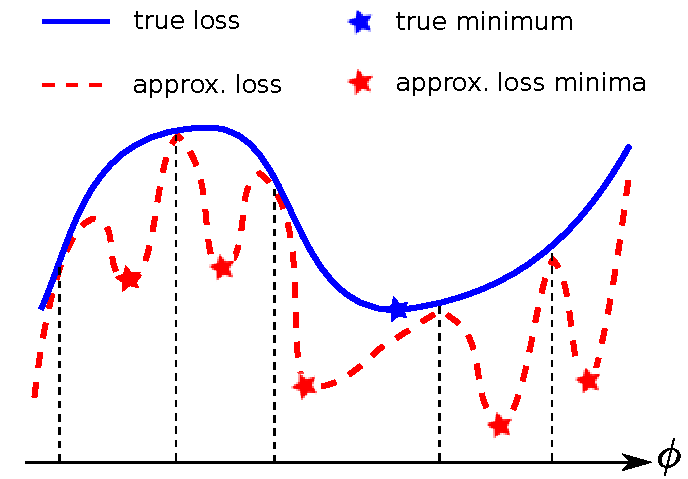
\includegraphics[width=0.5\linewidth]{Chapter5/approx_loss.pdf}
\caption{A visualisation of the exact/approximate loss. See main text for further intuition.}
\label{fig:chap_wild_loss_pathology}
\end{figure}

Here are two concrete examples for further explanation.

\begin{itemize}
\item Variational EM as an approximation to MLE. \\
The VAE algorithm can be viewed as an approximate MLE procedure, with the maximum likelihood objective $\mathcal{L}(\mparam) = \mathbb{E}_{\data}[\log p_{\mparam}(\x)]$ approximated by the variational lower-bound $\hat{\mathcal{L}}(\mparam, \vparam) = \mathbb{E}_{\data}[\mathcal{L}_{\text{VI}}(q_{\vparam}(\z | \x); \x)]$. As shown in the mean-field example in Section \ref{sec:chap4_mean_field}, this would bias the generative model $p_{\mparam}(\z | \x)$ towards simple solutions, unless $q_{\vparam}(\z | \x)$ perfectly approximates the exact posterior which is rarely the case. This issue is related to the ``hidden unit over-pruning'' problem \citep{burda:iwae2016, sonderby:ladder_vae2016}: even when $\z$ is of relatively high dimensions like a hundred, the VAE algorithm would turn off many of them, and learn a model which effectively uses much fewer units.

\item GAN training. \\
Recently generative adversarial networks (GANs) \citep{goodfellow:gan2014} have attracted large attention from the deep learning community. In a nutshell, the original GAN algorithm proposes training the generator $p_{\mparam}(\x)$ by minimising the Jensen-Shannon divergence
\begin{equation}
\min_{\mparam} \mathcal{L}(\mparam) = \mathrm{JS}[p_{\data} || p_{\mparam}] = \frac{1}{2} \mathrm{KL}\left[ p_{\data} || \frac{p_{\data} + p_{\mparam}}{2} \right] + \frac{1}{2} \mathrm{KL}\left[ p_{\mparam} || \frac{p_{\data} + p_{\mparam}}{2} \right].
\end{equation}
However, the generative model $p_{\mparam}(\x)$ is implicitly defined in an analogous way as the deterministic transform discussed above. Thus point-wise evaluation of $p_{\mparam}(\x)$ is intractable. Then the seminal GAN paper proposes approximating the Jenson-Shannon divergence \citep{lin:jensen_shannon1991} with a variational lower-bound, described by a \emph{discriminator}:
\begin{equation}
\min_{\mparam} \max_{\vparam} \hat{\mathcal{L}}(\mparam, \vparam) = \mathbb{E}_{\data} [\log D_{\vparam}(\x)] + \mathbb{E}_{p_{\mparam}} [\log (1 - D_{\vparam}(\x))].
\label{eq:chap5_original_gan}
\end{equation}
\cite{arjovsky:gan_problems2017} pointed out a fundamental problem with this approach: since both $p_{\data}$ and $p_{\mparam}$ have low-dimensional support in a high-dimensional space, the discriminator, if powerful enough (which is typically the case when using neural networks), is very likely to overfit, thus it can perfectly separate the two support sub-spaces and provide meaningless gradients. Then in their follow-up work \cite{arjovsky:wgan2017} proposed the Wasserstein GAN (WGAN), which uses Wasserstein distance \citep{villani:optimal_transport2008} as the training objective, and in this case, the approximate loss function turns out to be
\begin{equation}
\min_{\mparam} \max_{\vparam: || D_{\vparam}||_L \leq 1} \hat{\mathcal{L}}(\mparam, \vparam) = \mathbb{E}_{\data} [D_{\vparam}(\x)] - \mathbb{E}_{p_{\mparam}} [D_{\vparam}(\x)].
\label{eq:chap5_wgan}
\end{equation}
This modification, when adding more tricks to enforce the constraint $|| D_{\vparam}||_L \leq 1$ such as a gradient penalty \citep{gulrajani:wgan_gp2017}, has largely solved the instability issue of GAN training.

Another interesting explanation for why WGAN works is that the power of the discriminator, or the test function $D_{\vparam}$, has been restrained. On the other hand, in the original GAN case, over-fitting frequently happens, particularly at the beginning of training, as neural network classifiers can easily fit almost any data, even that with random labels as claimed by \cite{zhang:understanding2017}. Since smoothness is typically lost when over-fitting appears, it leads to poor approximations to the actual gradient and then a bad-performing model. Indeed \cite{kodali:dragan2017} also showed that the original GAN training can be stabilised when the discriminator is also constrained to be $1$-Lipschitz. 

\end{itemize}

From the above two examples, we see that the energy approximation approach can be problematic if not done in a correct way, therefore a \emph{direct gradient approximation} to the exact gradient might be preferred. There exists a rich literature on (non-parametric) derivative estimation \citep{stone:spline1985, zhou:spline2000, ruppert:lpr1994, fan:local_poly1996, debrabanter:lpr2013}; however, many of them require at least a noisy version of $\log q$ at the sampled locations, which is intractable in our case. Instead, \cite{singh:kernel_gradient1977} applied a kernel estimator directly to the first and higher order derivatives, and \cite{sasaki:gradient2015} improved upon this idea by performing kernel ridge regression directly on the derivatives. 
%
Also \cite{hyvarinen:score2005} considered score matching methods for approximating $\nabla_{\z} \log q(\z | \x)$, where follow-up papers \citep{sasaki:gradient2014, strathmann:kmc2015} derived kernel-based solutions and applied them to tasks such as approximate Bayesian computation (ABC) \citep{beaumont:abc2002}.
%
The core idea of these methods is the use of integration by parts to avoid evaluations of the actual gradients, making them applicable in our context. In Chapter \ref{chap:grad_approx} we will further discuss gradient approximation techniques and propose new gradient estimators for implicit models and wild approximate inference.

\vspace{1em}
\begin{tcolorbox}
\textbf{Remark} (denoising auto-encoder as a score function estimator)\textbf{.}
It has been shown in \citet{sarela:denoising2005, alain:denoising2014} that denoising auto-encoders (DAEs) \citep{vincent:denoising2008}, once trained, can be used to compute the score function approximately. Briefly speaking, a DAE learns to reconstruct a datum $\x$ from a corrupted input $\tilde{\x} = \x + \sigma \bm{\epsilon}, \bm{\epsilon} \sim \mathcal{N}(\bm{0}, \mathbf{I})$ by minimising the mean square error. Then the optimal DAE can be used to approximate the score function as $\nabla_{\x} \log p(\x) \approx \frac{1}{\sigma^2} (\text{DAE}^*(\x) - \x)$. \cite{sonderby:mapsr2016} deployed this idea to train an implicit model for image super-resolution, providing some promising results in some metrics. However applying similar ideas to variational inference can be very expensive, because the estimation of $\nabla_{\z} \log q(\z | \x)$ is a sub-routine for VI which is repeatedly required.
\end{tcolorbox}

\subsection{New optimisation objectives}
In variational inference, the KL-divergence $\mathrm{KL}[q||p]$ is minimised to obtain the approximate posterior. In general, the KL-divergence minimisation can be replaced by other optimisation-based approximation methods, as long as with the guarantee of recovering the exact posterior if $\mathcal{Q}$ contains it. However simply replacing the objective with some other $f$-divergence \citep{csiszar:divergence1963, morimoto:divergence1963, ali:divergence1966} does not simplify the problem as $q$ has an intractable density. Variational and adversarial techniques for estimating $f$-divergences \citep{nguyen:divergence2007, nguyen:divergence2010, nowozin:fgan2016} do not apply either, as the exact posterior is difficult to sample. 

One promising direction is to replace the KL divergence with Stein discrepancy \citep{stein:stein_method1972, barbour:stein_method1988, gorham:stein_method2015}, which has a special form that does not require evaluating $q$ nor sampling from $p$. 
Briefly speaking, Stein discrepancy involves a linear functional operator $\mathbf{O}_p$, called Stein operator, on a set of test functions $\mathcal{H} = \{ h(\z) \}$ such that $\mathbb{E}_{p(\bm{z}|\bm{x})}[(\mathbf{O}_p h)(\bm{z})] = 0$ for $\forall h \in \mathcal{H}$. Then the associated \emph{Stein discrepancy} is defined as $\mathcal{S}(q,  p) = \sup_{h \in \mathcal{H}} \mathbb{E}_{q}[(\mathbf{O}_p h)(\bm{z})]$. 
For continuous density functions, a generic Stein operator derived from Stein's identity \citep{stein:stein_method1972, stein:stein_method_multi1981} is $(\mathbf{O}_p h)(\z) = \nabla_{\z}\log p(\z, \x) h(\z) + \langle \nabla, h(\z) \rangle$, for which $\mathbb{E}_{p(\bm{z}|\bm{x})}[(\mathbf{O}_p h)(\bm{z})] = 0$. Putting them together, we have the Stein discrepancy (equipped with norm $|| \cdot ||$) \citep{gorham:stein_method2015}
\begin{equation}
\mathcal{S}(q, p) = \sup_{h \in \mathcal{H}} || \mathbb{E}_{q} [ \nabla_{\z}\log p(\z, \x) h(\z) + \langle \nabla, h(\z) \rangle ] ||,
\label{eq:chap5_stein_discrepancy}
\end{equation}
which only requires samples from $q$ and the score function $\nabla_{\z} \log p(\z, \x)$ and is thus indeed tractable.

Very recently Stein's method has been introduced to the approximate inference community. \cite{ranganath:ovi2016} defined $\mathcal{H}$ as parametric functions represented by neural networks, and obtained an approximate posterior by solving $\min_{q} \mathcal{S}(q, p)$. The authors approximated the minimax optimisation with gradient descent in an analogous way to GAN training \citep{goodfellow:gan2014}. In contrast, analytic solution of the supremum in (\ref{eq:chap5_stein_discrepancy}) exists if $\mathcal{H}$ is defined as the unit ball in an RKHS, where \cite{liu:ksd2016} and \cite{chwialkowski:ksd2016} termed the corresponding measure as the kernelised Stein discrepancy (KSD) that will be further discussed in Chapter \ref{chap:grad_approx}. \cite{liu:two_wild2016} further developed an approximate inference algorithm by directly minimising the KSD between the exact and approximate posterior distributions.

\subsection{Amortising stochastic dynamics}
MCMC and particle-based approximate inference methods \citep{dai:pmd2015, liu:svgd2016}, though very accurate, become inefficient when inference from multiple different distributions is repeatedly required. As an example consider learning a (deep) generative model, where fast (approximate) marginalisation of latent variables is desirable. Here we consider amortised inference to learn an inference network to mimic a selected stochastic dynamics. More precisely, we sample $\z \sim q(\z|\x)$, simulate $T$-step stochastic dynamics to obtain the updated particle $\z_{T}$, and update the $q$ distribution to ``catch-up'' those updated particles. For example, \cite{wang:amortisedsvgd2016} used this idea to amortise a deterministic dynamics called Stein variational gradient descent (SVGD) \citep{liu:svgd2016}, where the ``catch-up'' step is defined by deliberately chaining the gradients $\bm{\phi} \leftarrow \bm{\phi} + \epsilon \mathbb{E}_{q} [ \nabla_{\bm{\phi}} \bm{z} (\z_T - \z) ] $. In  \citet{li:amcmc2017} we extended this principle to MCMC methods and introduced different update rules for the (implicit) $q$ distribution. The theoretical intuition behind this approach is illustrated in Figure \ref{fig:chap5_amc_cartoon}. Since the MCMC ``oracle'' always improves the sample quality in terms of approximating the target distribution, by following the MCMC dynamics, the $q$ distribution will also get improved, until the stage when $\z_T$ has the same distribution as $\z$ which means $q = p$. Similar intuition also applies to other deterministic dynamics as long as they generate particles that are always approaching to the target distribution.

\begin{figure}
\centering
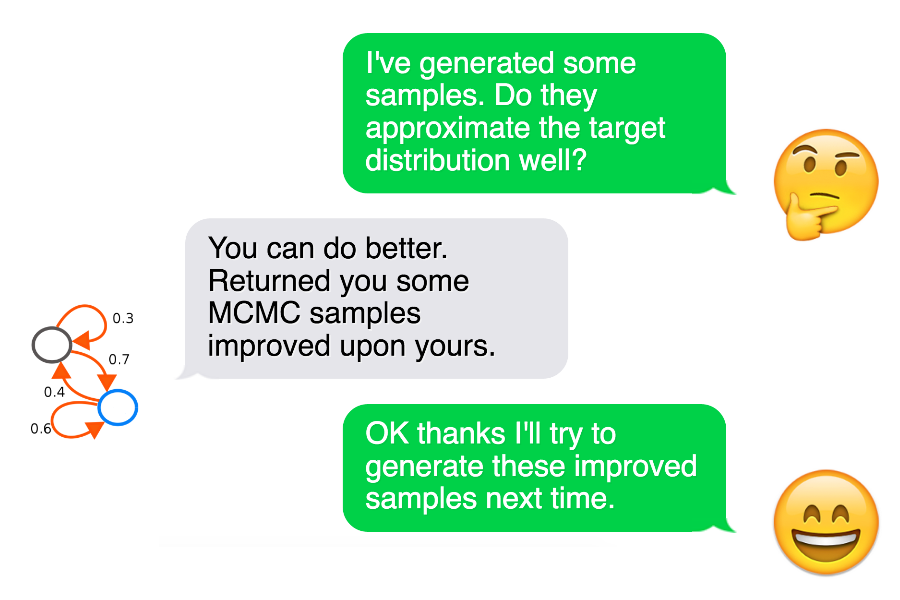
\includegraphics[width=0.6\linewidth]{Chapter5/amccartoon.png}
\caption{A cartoon illustration of the amortised MCMC idea in \cite{li:amcmc2017}. }
\label{fig:chap5_amc_cartoon}
\end{figure}



\section{Application: meta-learning for approximate inference}
\label{sec:chap5_wild_applications}

Many inference algorithms discussed in this thesis, e.g.~variational inference (with KL or R{\'e}nyi divergences) and sampling (importance sampling, SMC, MCMC, etc.), are designed as generic algorithms that can be directly applied to any integration problem. Can we automate the design of inference algorithms that are tailored to specific types of machine learning tasks (e.g.~Bayesian neural network regression)? In this section we briefly discuss a meta-learning \citep{schmidhuber:thesis1987, bengio:meta1992, naik:meta1992, thrun:meta1998} approach towards this goal.
%
The research scope of meta-learning is very broad, but in general the idea is to train a \emph{learner} on one or multiple tasks, in order to acquire common knowledge on \emph{how} to learn and generalise the learner to future tasks. Therefore meta-learning enables an inference algorithm to exploit commonly shared dependencies in a class of densities (say the posterior distribution of Bayesian neural network weights), and it is expected to produce a better approximation to the exact posterior.

In approximate inference context we define a learner as an algorithm $\mathcal{A}: \mathcal{P} \rightarrow \mathcal{Q}$ that maps the target distribution $p \in \mathcal{P}$ to an approximate distribution $q \in \mathcal{Q}$. For example, the classic variational inference algorithm can be rewritten as
\begin{equation}
\mathcal{A}_{\text{VI}}(p(\z | \x)) = \argmax_{q \in \mathcal{Q}} \mathbb{E}_q \left[ \log \frac{p(\x, \z)}{q(\z)} \right].
\end{equation}
Also the $T$-step simulation of an MCMC procedure with kernel $\mathcal{T}$ and initial distribution $q_0(\z | \x)$ is 
\begin{equation}
\mathcal{A}_{\mathcal{T}, T, q_0}(p(\z | \x)) = \int \mathcal{T}_T(\z | \z') q_0(\z' | \x) d\z' .
\end{equation}
Often these algorithms are approximated executed, e.g.~for variational inference the maximisation operator is approximated by $T$-step gradient ascent.

We consider meta-learning for approximate inference, which optimises $\mathcal{A}$ on a set of training densities $\{ p_n(\z) \}_{n=1}^N$, and generalises the learned algorithm $\mathcal{A}^*$ to unseen distributions. The training densities might come from a multi-task learning set-up, i.e.~$p_n(\z) = p(\z | \data_n)$ where $\data_n$ is the dataset for task $n$. Then one can define $\mathcal{A}(p(\z | \data)) = q_{\vparam}(\z | \data)$ with e.g.~a neural network, and then optimise the associated variational parameters $\vparam$ on the datasets $\data_1, ..., \data_N$. Further approximation techniques such as coresets \citep{huggins:coresets2016} and inducing points \citep{snelson:sparse_gp2006} can also be utilised If the dataset $\data_n$ is very big. In this case meta-learning for approximate inference algorithms can be viewed as amortised inference on \emph{task} level, therefore many of the recently developed techniques can be deployed. But it might require the use of techniques discussed in previous sections, as one might prefer the learned algorithm $\mathcal{A}$ to produce implicit posterior approximations to the target densities.

In general the $p_n$ densities might be derived from different probabilistic models with different observations and different latent variables, and the above neural network parameterisation is very likely to be sub-optimal. Instead of directly parameterising the $q$ distributions, we propose learning an approximate inference algorithm $\mathcal{A}_{\vparam}$ based on optimisation and/or sampling. 
%
%The first proposal takes inspirations from $f$-divergences \citep{csiszar:divergence1963} and the recently proposed perturbative variational objective \citep{bamler:perturbative_bbvi2017} that provides a lower-bound to the log marginal $\log p_n(\data_n)$:
%\begin{equation}
%\mathcal{A}_{f}(p_n(\z | \data_n)) = \argmax_{q \in Q} \ \mathbb{E}_q \left[ \log f \left( \frac{p_n(\data_n, \z)}{q(\z)} \right) \right]
%\end{equation}
%subject to that $f$ is a concave function on $\mathbb{R}^{+}$. A meta-learning approach would parameterise $f(\cdot) = f_{\vparam}(\cdot)$ and learn the parameters $\vparam$ by optimising some meta-objective $\mathcal{L}_{\text{meta}}$ on $\mathcal{A}_{f_{\vparam}}(p_n(\z | \data_n))$ for all $n = 1, ..., N$. Thus the learned variational objective will encourage the $q$ distribution to have desirable properties, e.g.~better interpolation between mode-seeking and mass-covering behaviours.
%
Consider learning a Markov process for posterior inference as an example. By parameterising $\mathcal{T}_n(\z'_n | \z_n) = \mathcal{T}_{\vparam}(\z'_n | \z_n; p_n)$ for all $n = 1, ..., N$, the sampler is learned by optimising some meta-objective $\mathcal{L}_{\text{meta}}$ on $\mathcal{A}_{\mathcal{T}_{\vparam}, T, q_0}(p_n(\z_n))$ for all $n = 1, ..., N$. 
%
Thus the trained transition kernel $\mathcal{T}_{\vparam}$ will have its stationary distribution close to the target $p_n$, and/or it will have fast convergence and low bias properties if $\mathcal{T}_{\vparam}(\z'_n | \z_n; p_n)$ is implicitly defined by a diffusion process with $p_n$ as the stationary distribution \citep{ma:mcmc_recipe2015}. The design of the meta-objective $\mathcal{L}_{\text{meta}}$ should avoid evaluating the density of the approximate posterior as an MCMC algorithm typically returns an implicit distribution. An initial experiment for learning samplers is presented in Chapter \ref{chap:grad_approx}.




\section{Summary}
We presented \emph{wild approximate inference} as a new research area within approximate inference. We established this area by investigating the fundamental question of what constitutes tractable approximate inference, and discussed potential restrictions introduced by both analytical approximate posteriors and conventional sampling methods. Then we provided examples of implicit approximations, and briefly discussed four algorithmic options for fitting them. Note that the recipes provided here are still mostly incomplete, and I must have missed many creative solutions developed by other researchers very recently. Nevertheless, it seems reasonable to believe that elucidating existing problems and pointing new research directions would help the community develop better approximate inference methods, thus leading to better Bayesian modelling.

%
In the next chapter, I will present one of our recent work that follows the gradient approximation proposal for wild approximate inference. There we will propose a new estimator of the score function $\nabla_{\z} \log q(\z | \x)$, and evaluate its approximating accuracy by considering applications in Bayesian deep learning. 
%\include{Chapter6/chapter6}
\chapter{Gradient Estimators for Implicit Models}
\label{chap:grad_approx}

% **************************** Define Graphics Path **************************
\ifpdf
    \graphicspath{{Chapter7/figs/Raster/}{Chapter7/figs/PDF/}{Chapter7/figs/}{Chapter7/}}
\else
    \graphicspath{{Chapter7/figs/Vector/}{Chapter7/figs/}{Chapter7/}}
\fi

%\section{Introduction}
%\label{sec:intro}

Modelling is fundamental to the success of technological innovations for artificial intelligence. A powerful model learns a useful representation of the observations for a specified prediction task, and generalises to unknown instances that follow similar generative mechanics. 
%
A well established area of machine learning research focuses on developing \emph{prescribed probabilistic models} \citep{diggle:prescribe_implicit1984}, where learning is based on evaluating the probability of observations under the model. \emph{Implicit probabilistic models}, on the other hand, are defined by a stochastic procedure that allows for direct generation of samples, but not for the evaluation of model probabilities. These are omnipresent in scientific and engineering research involving data analysis, for instance ecology, climate science and geography, where simulators are used to fit real-world observations to produce forecasting results. 

Within the machine learning community, there is a recent interest in a specific type of implicit models, generative adversarial networks (GANs) \citep{goodfellow:gan2014}, which has been shown to be one of the most successful approaches to image generation \citep{radford:dcgan2016, arjovsky:wgan2017, berthelot:began2017}. Very recently, implicit distributions have also been considered as approximate posterior distributions for Bayesian inference, e.g.~see discussions in the last chapter and recent papers including \citet{liu:two_wild2016, wang:amortisedsvgd2016, karaletsos:adversarial_mp2016, mescheder:avb2017, huszar:implicit2017, li:amcmc2017, tran:implicit2017, shi:kivi2018}. These examples demonstrate the superior flexibility of implicit models, which provide highly expressive means of modelling complex data structures.


%Many machine learning papers mainly focus on developing \emph{prescribed probabilistic models} \citep{diggle:prescribe_implicit1984} for their tasks, where learning is usually done by evaluating the probability of observations under the model. However, \emph{implicit probabilistic models}, which are defined by a stochastic procedure that directly generates samples, have also attracted major attention. In many scientific fields that involve data analysis, for instance ecology, climate science and geography, simulators are commonly used to fit the real-world data and produce forecasting results. Another example of such implicit models are generative adversarial networks (GAN) \citep{goodfellow:gan2014} which have been shown to be one of the most successful approaches to image and text generation \citep{radford:dcgan2016, yu:seqgan2017, arjovsky:wgan2017, berthelot:began2017}. Very recently, implicit distributions have also been considered as approximate posterior distributions for Bayesian inference, e.g.~see \citep{liu:two_wild2016, wang:amortise_svgd2016, li:wild2016, karaletsos:adversarial_mp2016, mescheder:avb2017, huszar:implicit2017, li:amcmc2017, tran:implicit2017}. These examples demonstrate the superior flexibility of implicit models, which are highly expressive in modelling many data structures.

Whilst prescribed probabilistic models can be learned by standard (approximate) maximum likelihood or Bayesian inference, implicit probabilistic models require substantially more severe approximations due to the intractability of the model distribution. Many existing approaches first approximate the model distribution or optimisation objective function and then use those approximations to learn the associated parameters. However, such approximation can lead to unstable training and poor results, where a prevalent example is the original GAN framework \citep{goodfellow:gan2014} that has been briefly sketched in Section \ref{sec:chap5_grad_approx}.
%
Recent ideas to address this issue for GANs suggest that restricting the representational power of the discriminator is effective in stabilising training \citep[e.g. see][]{arjovsky:wgan2017, kodali:dragan2017}. However, such restrictions, if not carefully crafted, often introduce undesirable biases, responsible for problems such as mode collapse in the context of GANs, and uncertainty underestimation in variational inference methods \citep{turner:two_problems2011}.

\begin{figure}
\subfigure[approximate loss function \label{fig:approx_loss}]{
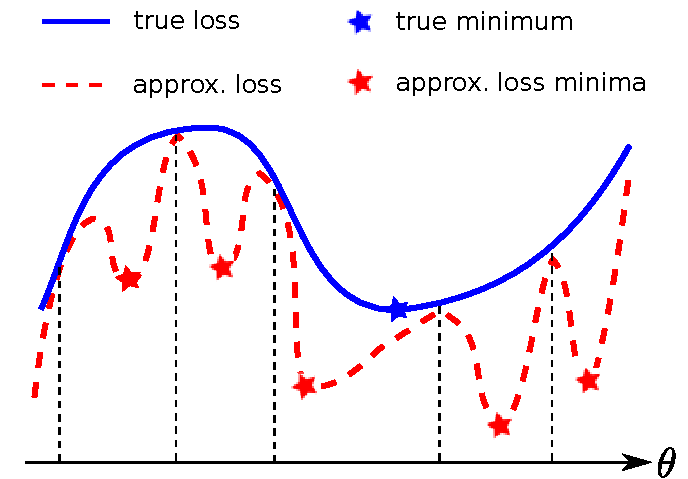
\includegraphics[width=0.45\linewidth]{figs/approx_loss.pdf}}
\hfill
\subfigure[approximate gradients \label{fig:approx_gradient}]{
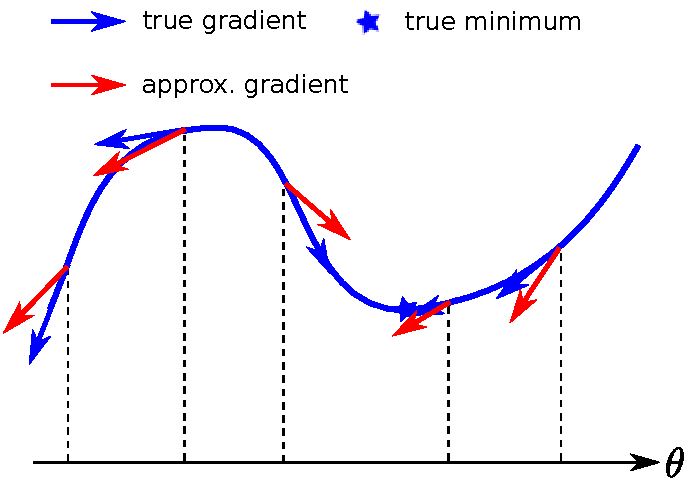
\includegraphics[width=0.45\linewidth]{figs/approx_gradient.pdf}}
\caption{A comparison between the two approximation schemes. Since in practice the optimiser only visits finite number of locations in the parameter space, it can lead to over-fitting if the neural network based functional approximator is not carefully regularised, and therefore the curvature information of the approximated loss can be very different from that of the original loss (shown in (a)). On the other hand, the gradient approximation scheme (b) can be more accurate since it only involves estimating the sensitivity of the loss function to the parameters in a local region.}
\label{fig:loss_grad_approx_compare}
\end{figure}

%Whilst prescribed probabilistic models can be learned by standard approximate maximum likelihood or Bayesian inference, implicit probabilistic models require more severe approximations due to the intractability of the model distribution. Many existing approaches first approximate the model distribution and/or optimisation objective functions, then learn the associated parameters using the defined approximations. For example, GANs use a discriminator which serves as a critic of the generative model, and let both networks play a minimax game until convergence. However, for finite number of data-points, there are infinite number of functions that could perfectly approximate the exact objective function evaluated at those observations, and for some of these approximating functions the gradient directions can be arbitrary far away from the exact ones. This is especially true when the approximated objective function is represented by neural network critics, where recent advances for stabilising GANs suggest restricting the representation power of the discriminator (e.g. see \citep{arjovsky:wgan2017}). There exist similar issues for variational methods as well, i.e.~proposing a lower-bound/upper-bound to the exact loss function. Similar to the variational lower-bound, these bounds are unlikely to be equally tight everywhere \citep{turner:two_problems2011}. It often biases the approximate posterior towards under-estimating uncertainty, and similarly for GANs the same problem exists as mode collapsing.

In the previous chapter a number of proposals for wild approximate inference are presented. Critically, we believe these techniques are extendable to learning implicit models, and in this chapter we explore the \emph{direct gradient approximation} idea as an alternative. A visualisation of the two approximation schemes is provided in Figure \ref{fig:loss_grad_approx_compare}. More specifically we focus on approximating the score function, in which an accurate approximation of it then allows the application of many well-studied algorithms, such as maximum likelihood, maximum entropy estimation, variational inference and gradient-based MCMC, to implicit models. Concretely, our contributions include:  
\begin{itemize}
\item the \emph{Stein gradient estimator}, a novel generalisation of the score matching estimator \citep{hyvarinen:score2005}, with both parametric and non-parametric versions;
\item a comparison of the proposed estimator with the score matching and the KDE plug-in estimators on performing gradient-free MCMC, meta-learning of approximate posterior samplers for Bayesian neural networks, and entropy based regularisation of GANs.
\end{itemize}

%In this paper we explore an alternative idea of training implicit models, which directly approximates the gradient of the implicit model distribution. More precisely we focus on approximating the score function $\nabla_{\x} \log q(\x)$ for some distribution $q$ to be learned. The score function is widely used in machine learning algorithms, e.g.~maximum likelihood, variational inference and gradient-based MCMC. Hence an accurate approximation to the score function would enable the application of these well-studied algorithms to implicit models. After reviewing recent advances in implicit models and gradient approximation techniques, we make the following contributions:  
%\begin{itemize}
%\item We propose the \emph{Stein gradient estimator} as a novel generalisation of the score matching estimator \citep{hyvarinen:score2005}, with both parametric and non-parametric versions presented;
%\item We compare the Stein estimator with the score matching estimator and the KDE plug-in estimator on three different tasks: gradient-free MCMC, entropy regularised GANs, and meta-learning of approximate posterior samplers for Bayesian neural networks.
%\end{itemize}

\section{Learning implicit probabilistic models}

Given a dataset $\mathcal{D}$ containing i.i.d.~samples we would like to learn a probabilistic model $p(\x)$ for the underlying data distribution $p_{\data}(\x)$. In the case of implicit models, $p(\x)$ is defined by a generative process. For example, to generate images, one might define a generative model $p(\x)$ that consists of sampling randomly a latent variable $\z \sim p_0(\z)$ and then defining $\x = \f_{\mparam}(\z)$. Here $\f$ is a function parametrised by $\mparam$, usually a deep neural network or a simulator. We assume $\f$ to be differentiable w.r.t.~$\mparam$. An extension to this scenario is presented by \emph{conditional} implicit models, where the addition of a supervision signal $\y$, such as an image label, allows us to define a conditional distribution $p(\x| \y)$ implicitly by the transformation $\x = \f_{\mparam}(\z, \y)$. A related methodology, \emph{wild approximate inference} (Chapter \ref{chap:wild}) assumes a tractable joint density $p(\x, \z)$, but uses implicit proposal distributions to approximate an intractable exact posterior $p(\z|\x)$. Here the approximate posterior $q(\z|\x)$ can likewise be represented by a deep neural network, but also by a truncated Markov chain, such as that given by Langevin dynamics with learnable step-size. 

%Given a dataset $\mathcal{D}$ containing i.i.d.~samples of the data distribution $p_{\data}(\x)$, we would like to learn it with a probabilistic model $p(\x)$. Implicit models usually define this distribution by describing a generative process. Taking image generation as an example, the generative model $p(\x)$ is defined by first sampling some random configuration of a latent variable $\z \sim p_0(\z)$, then transforming it into $\x = \f_{\mparam}(\z)$ with a function $\f$ parametrised by $\mparam$. In the rest of the paper we assume $\f$ is differentiable w.r.t.~$\mparam$. Such function can be represented by a deep neural network or a simulator. \emph{Conditional} implicit models have also been studied in the literature, for example, one can add in supervision signals $\y$, e.g.~labels of the image, and define $p(\x| \y)$ implicitly by the transformation $\x = \f_{\mparam}(\z, \y), \z \sim p_0(\z)$. On the other hand, \emph{wild variational inference} \citep{liu:two_wild2016, li:wild2016} assumes a tractable joint density $p(\x, \z)$ but proposes using implicit distributions to approximate the intractable exact posterior $p(\z|\x)$. Here the approximate posterior $q(\z|\x)$ can also be represented by a deep neural network, or a truncated Markov chain such as Langevin dynamics with learnable step-size. 

Whilst providing extreme flexibility and expressive power, the intractability of density evaluation also brings serious optimisation issues for implicit models. This is because many learning algorithms, e.g.~maximum likelihood estimation (MLE), rely on minimising a distance/divergence/discrepancy measure $\mathrm{D}[p || p_{\data}]$, which often requires evaluating the model density \citep[c.f.][]{ranganath:ovi2016, liu:two_wild2016}. Thus good approximations to the optimisation procedure are the key to learning implicit models that can describe complex data structure. In the context of GANs, the Jensen-Shannon divergence is approximated by a variational lower-bound represented by a discriminator \citep{barber:vim2003, goodfellow:gan2014}. 
%
Related work for wild variational inference \citep{li:wild2016, mescheder:avb2017, huszar:implicit2017, tran:implicit2017} uses a GAN-based technique to construct a density ratio estimator for $q / p_0$ \citep{sugiyama:ratio2009, sugiyama:ratio2012, uehara:gan2016, mohamed:gan2016} and then approximates the KL-divergence term in the variational lower-bound:
\begin{equation}
\mathcal{L}_{\text{VI}}(q) = \mathbb{E}_{q} \left[ \log p(\x | \z) \right] - \mathrm{KL}[q_{\vparam}(\z|\x) || p_0(\z)].
\end{equation} 
In addition, \cite{li:wild2016} and \cite{mescheder:avb2017} exploit the additive structure of the KL-divergence and suggest discriminating between $q$ and an auxiliary distribution that is close to $q$, making the density ratio estimation more accurate. Nevertheless all these algorithms involve a minimax optimisation, and the current practice of gradient-based optimisation is notoriously unstable. 

The stabilisation of GAN training is itself a recent trend of related research \citep[e.g.~see][]{salimans:training2016, arjovsky:wgan2017}. However, as the gradient-based optimisation only interacts with gradients, there is no need to use a discriminator if an accurate approximation to the intractable gradients could be obtained. As an example, consider a variational inference task with the approximate posterior defined as $\z \sim q_{\vparam}(\z | \x) \Leftrightarrow \bm{\epsilon} \sim \pi(\bm{\epsilon}), \z = \f_{\vparam}(\bm{\epsilon}, \x)$. Notice that the variational lower-bound can be rewritten as
\begin{equation}
\mathcal{L}_{\text{VI}}(q) = \mathbb{E}_{q} \left[ \log p(\x, \z) \right]  + \mathbb{H}[q_{\vparam}(\z | \x)],
\label{eq:vi_objective_entropy}
\end{equation}
the gradient of the variational parameters $\vparam$ can be computed by a sum of the path gradient of the first term (i.e.~$\mathbb{E}_{\pi} \left[ \nabla_{\f} \log p(\x, \f(\noise, \x))^{\text{T}} \nabla_{\vparam} \f(\noise, \x) \right] $) and the gradient of the entropy term $\nabla_{\vparam} \mathbb{H}[q(\z | \x)]$. Expanding the latter, we have 
%\begin{equation}
%-\nabla_{\vparam} \mathbb{H}[q(\z | \x)] = \mathbb{E}_{\pi} \left[ \nabla_{\f} \log q(\f(\noise, \x) | \x)^{\text{T}} \nabla_{\vparam} \f(\noise, \x)] \right] + \mathbb{E}_{q} \left[ \nabla_{\vparam} \log q_{\vparam}(\z | \x) \right],
%\label{eq:entropy_gradient}
%\end{equation}
\begin{equation}
\begin{aligned}
\nabla_{\vparam} \mathbb{H}[q_{\vparam}(\z | \x)] 
&= - \nabla_{\vparam} \mathbb{E}_{\pi(\bm{\epsilon})}[\log q_{\vparam}(\f_{\vparam}(\bm{\epsilon}, \x))] \\
&= - \mathbb{E}_{\pi(\bm{\epsilon})}[ \nabla_{\vparam} \log q_{\vparam}(\f_{\vparam}(\bm{\epsilon}, \x))] \\
&= - \mathbb{E}_{\pi(\bm{\epsilon})}[ \nabla_{\vparam} \log q_{\vparam}(\z | \x) |_{\z = \f_{\vparam}(\bm{\epsilon}, \x)} +  \nabla_{\vparam} \f_{\vparam}(\bm{\epsilon}, \x)  \nabla_{\f} \log q_{\vparam}(\f_{\vparam}(\bm{\epsilon}, \x) | \x) ] \\
&= - \mathbb{E}_{q_{\vparam}(\z | \x)} [ \nabla_{\vparam} \log q_{\vparam}(\z | \x)] - \mathbb{E}_{\pi(\bm{\epsilon})} [ \nabla_{\vparam} \f_{\vparam}(\bm{\epsilon}, \x) \nabla_{\f} \log q_{\vparam}(\f_{\vparam}(\bm{\epsilon}, \x) | \x)  ],
\end{aligned}
\label{eq:entropy_gradient}
\end{equation}
in which the first term in the last line is zero \citep{roeder:sticking2017}. As we typically assume the tractability of $\nabla_{\vparam} \f$, an accurate approximation to $\nabla_{\z} \log q(\z | \x)$ would remove the requirement of discriminators, speed-up the learning and obtain potentially a better model.
%
Many gradient approximation techniques exist \citep{stone:spline1985, fan:local_poly1996, zhou:spline2000, debrabanter:lpr2013}, and in particular, in the next section we will review kernel-based methods such as kernel density estimation \citep{singh:kernel_gradient1977} and score matching \citep{hyvarinen:score2005} in more detail, and motivate the main contribution of this chapter.


\section{Gradient approximation with the Stein gradient estimator}
\label{sec:gradient_approximation}

We propose the \emph{Stein gradient estimator} as a novel generalisation of the score matching gradient estimator. Before presenting it we first set-up the notation. Column vectors and matrices are boldfaced. The random variable under consideration is $\x \in \mathcal{X}$ with $\mathcal{X} = \mathbb{R}^{d \times 1}$ if not specifically mentioned. To avoid misleading notation we use the distribution $q(\x)$ to derive the gradient approximations for general cases. As Monte Carlo methods are heavily used for implicit models, in the rest of the paper we mainly consider approximating the gradient $\g(\x^k) :=\nabla_{\x^k} \log q(\x^k)$ for $\x^k \sim q(\x), k = 1, ..., K$. We use $x^i_j$ to denote the $j$th element of the $i$th sample $\x^i$. We also denote the matrix form of the collected gradients as
$\Grad := \left( \nabla_{\x^1} \log q(\x^1), \cdots, \nabla_{\x^K} \log q(\x^K) \right)^{\text{T}} \in \mathbb{R}^{K \times d}$, and its approximation $\hat{\Grad} := \left( \hat{g}(\x^1), \cdots, \hat{g}(\x^K) \right)^{\text{T}}$ with $\hat{g}(\x^k) = \nabla_{\x^k} \log \hat{q}(\x^k)$ for some $\hat{q}(\x)$.

\subsection{Stein gradient estimator: inverting Stein's identity}
We start from introducing \emph{Stein's identity} that was first developed for Gaussian random variables \citep{stein:stein_method1972, stein:stein_method_multi1981} then extended to general cases \citep{gorham:stein_method2015, liu:ksd2016}.
%
Let $\h: \mathbb{R}^{d \times 1} \rightarrow \mathbb{R}^{d' \times 1}$ be a differentiable multivariate test function which maps $\x$ to a column vector $\h(\x) = [h_1(\x), h_2(\x), ..., h_{d'}(\x)]^{\text{T}}$. We further assume the \emph{boundary condition} for $\h$: 
\begin{equation}
q(\x)\h(\x) |_{\partial \mathcal{X}} = \bm{0}, \text{ or } \lim_{\x \rightarrow \bm{\infty}} q(\x) \h(\x) = 0 \text{ if } \mathcal{X} = \mathbb{R}^d.
\label{eq:boundary_condition}
\end{equation}
This condition holds for almost any test function if $q$ has sufficiently fast-decaying tails (e.g.~Gaussian tails).
%
Now we introduce Stein's identity \citep{stein:stein_method_multi1981, gorham:stein_method2015, liu:ksd2016}
\begin{equation}
\mathbb{E}_{q}[\h(\x) \nabla_{\x} \log q(\x)^{\text{T}} + \nabla_{\x} \h(\x) ] = \bm{0}, 
\label{eq:stein_identity_multi}
\end{equation}
in which the gradient matrix term
$
\nabla_{\x} \h(\x) = \left( \nabla_{\x} h_1(\x), \cdots, \nabla_{\x} h_{d'}(\x) \right)^{\text{T}} \in \mathbb{R}^{d' \times d}.
$
This identity can be proved using \emph{integration by parts}: for the $i$th row of the matrix $\h(\x) \nabla_{\x} \log q(\x)^{\text{T}}$, we have
\begin{equation}
\begin{aligned}
\mathbb{E}_{q}[ h_i(\x) \nabla_{\x} \log q(\x)^{\text{T}}]
&= \int h_i(\x) \nabla_{\x} q(\x)^{\text{T}} d \x \\
&= q(\x)h_i(\x) |_{\partial \mathcal{X}} - \int q(\x)  \nabla_{\x} h_i(\x)^{\text{T}} d \x \\
&= - \mathbb{E}_{q} [\nabla_{\x} h_i(\x)^{\text{T}}].
\end{aligned}
\label{eq:integration_by_parts}
\end{equation}
Observing that the gradient term $\nabla_{\x} \log q(\x)$ of interest appears in Stein's identity (\ref{eq:stein_identity_multi}), we propose the \emph{Stein gradient estimator} by inverting Stein's identity. As the expectation in (\ref{eq:stein_identity_multi}) is intractable, we further approximate the above with Monte Carlo (MC):
\begin{equation}
\frac{1}{K} \sum_{k=1}^K -\h(\x^k) \nabla_{\x^k} \log q(\x^k)^{\text{T}} + \text{err} = \frac{1}{K} \sum_{k=1}^K \nabla_{\x^k} \h(\x^k), \quad \x^k \sim q(\x^k),
\label{eq:stein_multi_mc}
\end{equation}
with $\text{err} \in \mathbb{R}^{d' \times d}$ the random error due to MC approximation, which has mean $\bm{0}$ and vanishes as $K \rightarrow +\infty$. Now by temporarily denoting
$$
\Hmatrix = \left( \h(\x^1), \cdots , \h(\x^K) \right) \in \mathbb{R}^{d' \times K}, \quad
\hgrad = \frac{1}{K} \sum_{k=1}^K \nabla_{\x^k} \h(\x^k) \in \mathbb{R}^{d' \times d},
$$
equation (\ref{eq:stein_multi_mc}) can be rewritten as
$$-\frac{1}{K} \Hmatrix \Grad + \text{err} = \hgrad.$$
Thus we consider a ridge regression method (i.e. adding an $\ell_2$ regulariser) to estimate $\Grad$:
\begin{equation}
\hat{\Grad}_V^{\text{Stein}} := \argmin_{\hat{\Grad} \in \mathbb{R}^{K \times d} } || \hgrad + \frac{1}{K} \Hmatrix \hat{\Grad} ||_{F}^2 + \frac{\eta}{K^2} || \hat{\Grad} ||_{F}^2,
\label{eq:stein_objective}
\end{equation}
with $|| \cdot ||_{F}$ the Frobenius norm of a matrix and $\eta \geq 0$. Simple calculation shows that
\begin{equation}
\hat{\Grad}_V^{\text{Stein}} = -( \K + \eta \bm{I} )^{-1} \langle \nabla, \K \rangle,
\label{eq:stein_estimator}
\end{equation}
where 
$$\K := \Hmatrix^{\text{T}} \Hmatrix, \quad \K_{ij} = \mathcal{K}(\x^i, \x^j) := \h(\x^i)^{\text{T}} \h(\x^j),$$
$$\langle \nabla, \K \rangle := K \Hmatrix^{\text{T}} \hgrad, \quad \langle \nabla, \K \rangle_{ij} = \sum_{k=1}^{K} \nabla_{x^k_j} \mathcal{K}(\x^i, \x^k).$$
%
One can show that the RBF kernel satisfies Stein's identity \citep{liu:ksd2016}. In this case $\h(\x) = \mathcal{K}(\x, \cdot), d' = +\infty$ and by the reproducing kernel property  \citep{berlinet:rkhs2011},
$\h(\x)^{\text{T}} \h(\x') = \langle \mathcal{K}(\x, \cdot), \mathcal{K}(\x', \cdot) \rangle_{\mathcal{H}} = \mathcal{K}(\x, \x') .$

\subsection{Stein gradient estimator minimises the kernelised Stein discrepancy}
In this section we derive the Stein gradient estimator again, but from a divergence/discrepancy minimisation perspective. 
%
Stein's method also provides a tool for checking if two distributions $q(\x)$ and $\hat{q}(\x)$ are identical. If the test function set $\mathcal{H}$ (containing one-dimensional test functions $h \in \mathcal{H}$) is sufficiently rich, then one can define a Stein discrepancy measure (equipped with norm $|| \cdot ||$) by
\begin{equation}
\mathcal{S}(q, \hat{q}) := \sup_{\h \in \mathcal{H}} || \mathbb{E}_{q} \left[ \nabla_{\x} \log \hat{q}(\x) h(\x) + \nabla_{\x} h(\x) \right] ||,
\label{eq:stein_discrepancy}
\end{equation}
see \cite{gorham:stein_method2015} for an example derivation. The definition can be generalised to multi-dimension test functions $\h(\x)$, and in particular, when $\mathcal{H}$ is defined as a unit ball in an RKHS induced by a kernel $\mathcal{K}(\x, \cdot)$ and $|| \cdot ||$ is the $\ell_2$ norm, \cite{liu:ksd2016} and \cite{chwialkowski:ksd2016} showed that the supremum in (\ref{eq:stein_discrepancy}) can be analytically obtained as (recall $\g(\x) = \nabla_{\x} \log q(\x), \hat{\g}(\x) = \nabla_{\x} \log \hat{q}(\x)$): 
\begin{equation}
\mathcal{S}^2(q, \hat{q}) = \mathbb{E}_{\x, \x' \sim q} \left[ (\hat{\g}(\x) - \g(\x) )^{\text{T}} \mathcal{K}(\x, \x') (\hat{\g}(\x') - \g(\x') ) \right],
\label{eq:ksd}
\end{equation}
which is also named the \emph{kernelised Stein discrepancy} (KSD). \cite{chwialkowski:ksd2016} showed that for $C_0$-universal kernels satisfying the boundary condition, KSD is indeed a discrepancy measure: $\mathcal{S}^2(q, \hat{q}) = 0 \Leftrightarrow q = \hat{q}$.  \cite{gorham:ksd2017} further characterised the power of KSD on detecting non-convergence cases. Furthermore, if the kernel is twice differentiable, then using the same technique as to derive (\ref{eq:score_matching_objective}) one can compute KSD by  (with $\mathcal{K}_{\x \x'}$ shorthand for $\mathcal{K}(\x, \x')$):
\begin{equation}
\mathcal{S}^2(q, \hat{q}) = \mathbb{E}_{\x, \x' \sim q} \left[ \hat{\g}(\x)^{\text{T}} \mathcal{K}_{\x \x'} \hat{\g}(\x') + \hat{\g}(\x)^{\text{T}} \nabla_{\x'} \mathcal{K}_{\x \x'} + \nabla_{\x} \mathcal{K}_{\x \x'}^{\text{T}} \hat{\g}(\x') + \text{Tr}(\nabla_{\x, \x'} \mathcal{K}_{\x \x'} )\right].
\label{eq:ksd_transformed}
\end{equation}
In practice KSD is estimated with samples $\{ \x^k \}_{k=1}^K \sim q$, and simple derivations show that the V-statistic of KSD can be reformulated as $\mathcal{S}_{V}^2(q, \hat{q}) = \frac{1}{K^2} \text{Tr} (\hat{\Grad}^{\text{T}} \K \hat{\Grad} + 2 \hat{\Grad}^{\text{T}} \langle \nabla, \K \rangle) + C$.
%
Thus the $l_2$ error in (\ref{eq:stein_objective}) is equivalent to the V-statistic of KSD if $\h(\x) = \mathcal{K}(\x, \cdot)$, and we have the following:
\begin{theorem}
$\hat{\Grad}_V^{\text{\emph{Stein}}}$ is the solution of the following KSD V-statistic minimisation problem
\begin{equation}
\hat{\Grad}_V^{\text{\emph{Stein}}} = \argmin_{\hat{\Grad} \in \mathbb{R}^{K \times d}} \quad \mathcal{S}_{V}^2(q, \hat{q}) + \frac{\eta}{ K^2} ||\hat{\Grad}||_F^2 .
\end{equation}
\label{thm:stein_ksd}
\vspace{-0.2in}
\end{theorem}
%
One can also minimise the U-statistic of KSD to obtain gradient approximations, and a full derivation of which, including the optimal solution, can be found in Appendix \ref{sec:appendix_stein}. In experiments we use V-statistic solutions and leave comparisons between these methods to future work.

\subsection{Comparisons to existing kernel-based gradient estimators}
There exist other gradient estimators that do not require explicit evaluations of $\nabla_{\x} \log q(\x)$, e.g.~the denoising auto-encoder (DAE) \citep{vincent:denoising2008, vincent:denoising2011, alain:denoising2014} which, with infinitesimal noise, also provides an estimate of $\nabla_{\x} \log q(\x)$ at convergence. However, applying such gradient estimators result in a double-loop optimisation procedure since the gradient approximation is repeatedly required for fitting implicit distributions, which can be significantly slower than the proposed approach. Therefore we focus on ``quick and dirty'' approximations and only include comparisons to kernel-based gradient estimators in the following.

\subsubsection{KDE gradient estimator: plug-in estimator with density estimation}
A naive approach for gradient approximation would first estimate the intractable density $\hat{q}(\x) \approx q(\x)$ (up to a constant), then approximate the exact gradient by $\nabla_{\x} \log \hat{q}(\x) \approx \nabla_{\x} \log q(\x)$. Specifically, \cite{singh:kernel_gradient1977} considered kernel density estimation (KDE) 
$\hat{q}(\x) = \frac{1}{K} \sum_{k=1}^K \mathcal{K}(\x, \x^k) \times C.$, then differentiated through the KDE estimate to obtain the gradient estimator:
\begin{equation}
\hat{\Grad}^{\text{KDE}}_{ij} = \sum_{k=1}^K \nabla_{x^i_j} \mathcal{K}(\x^i, \x^k) / \sum_{k=1}^K \mathcal{K}(\x^i, \x^k).
\label{eq:kde_estimator}
\end{equation}
%
Interestingly for translation invariant kernels $\mathcal{K}(\x, \x') = \mathcal{K}(\x - \x')$ the \emph{KDE gradient estimator} (\ref{eq:kde_estimator}) can be rewritten as $\hat{\Grad}^{\text{KDE}} = -\text{diag}\left( \K \bm{1} \right)^{-1} \langle \nabla, \K \rangle.$
Inspecting and comparing it with the Stein gradient estimator (\ref{eq:stein_estimator}), one might notice that the Stein method uses the full kernel matrix as the pre-conditioner, while the KDE method computes an averaged ``kernel similarity'' for the denominator. We conjecture that this difference is key to the superior performance of the Stein gradient estimator when compared to the KDE gradient estimator (see later experiments). The KDE method only collects the similarity information between $\x^k$ and other samples $\x^j$ to form an estimate of $\nabla_{\x^k} \log q(\x^k)$, whereas for the Stein gradient estimator, the kernel similarity between $\x^i$ and $\x^j$ for all $i, j \neq k$ are also incorporated. Thus it is reasonable to conjecture that the Stein method can be more sample efficient, which also implies higher accuracy when the same number of samples are collected.

\subsubsection{Score matching gradient estimator: minimising MSE}
\label{sec:score_matching}
The KDE gradient estimator performs indirect approximation of the gradient via density estimation, which can be inaccurate. An alternative approach directly approximates the gradient $\nabla_{\x} \log q(\x)$ by minimising the expected $\ell_2$ error w.r.t.~the approximation $\hat{\g}(\x) = \left(\hat{g}_1(\x), \cdots, \hat{g}_d(\x) \right)^{\text{T}}$:
\begin{equation}
\mathcal{F}(\hat{\g}) := \mathbb{E}_{q} \left[ || \hat{\g}(\x) - \nabla_{\x} \log q(\x) ||_2^2 \right].
\label{eq:fisher_divergence}
\end{equation}
It has been shown in \cite{hyvarinen:score2005} that this objective can be reformulated as
\begin{equation}
\mathcal{F}(\hat{\g}) = \mathbb{E}_{q} \left[ || \hat{\g}(\x) ||_2^2 + 2 \langle \nabla, \hat{\g}(\x) \rangle \right] + C, \quad \langle \nabla, \hat{\g}(\x) \rangle = \sum_{j=1}^d \nabla_{x_j} \hat{g}_j(\x).
\label{eq:score_matching_objective}
\end{equation}
The key insight here is again the usage of integration by parts: after expanding the $\ell_2$ loss objective, the cross term can be rewritten as
$\mathbb{E}_q \left[ \hat{\g}(\x)^{\text{T}} \nabla_{\x} \log q(\x) \right] = -\mathbb{E}_q \left[ \langle \nabla, \hat{\g}(\x) \rangle \right],$
if assuming the boundary condition (\ref{eq:boundary_condition}) for $\hat{\g}$ (see (\ref{eq:integration_by_parts})). 
%
The optimum of (\ref{eq:score_matching_objective}) is referred as the \emph{score matching gradient estimator}. 
%
The $\ell_2$ objective (\ref{eq:fisher_divergence}) is also called \emph{Fisher divergence} \citep{johnson:itbook2004} which is a special case of KSD (\ref{eq:ksd}) by selecting $\mathcal{K}(\x, \x') = \delta_{\x = \x'}$. Thus the Stein gradient estimator can be viewed as a generalisation of the score matching estimator. 
%
%A slightly different approach \citep{sasaki:gradient2015} proposes an estimator for $\nabla_{\x} q(\x)$, by minimising the $l_2$ error $\int (\hat{g}_j(\x) - \nabla_{x_j} q(\x))^2 d\x$ and removing explicit calculations of $\nabla_{\x} q(\x)$ in an analogous way as to derive (\ref{eq:score_matching_objective}). 

The comparison between the two estimators is more complicated. Certainly by the Cauchy-Schwarz inequality the Fisher divergence is stronger than KSD in terms of detecting convergence \citep{liu:ksd2016}. However it is difficult to perform direct gradient estimation by minimising the Fisher divergence, since (i) the Dirac kernel is non-differentiable so that it is impossible to rewrite the divergence in a similar form to (\ref{eq:ksd_transformed}), and (ii) the transformation to (\ref{eq:score_matching_objective}) involves computing $\nabla_{\x} \hat{\g}(\x)$. So one needs to propose a \emph{parametric} approximation to $\Grad$ and then optimise the associated parameters accordingly, and indeed \cite{sasaki:gradient2014} and \cite{strathmann:kmc2015} derived a parametric solution by first approximating the log density up to a constant as
$\log \hat{q}(\x) := \sum_{k=1}^K a_k \mathcal{K}(\x, \x^k) + C$,
then minimising (\ref{eq:score_matching_objective}) to obtain the coefficients $\hat{a}^{\text{score}}_k$ and constructing the gradient estimator as
\begin{equation}
\hat{\Grad}^{\text{score}}_{i\cdot} = \sum_{k=1}^{K} \hat{a}^{\text{score}}_k \nabla_{\x^i} \mathcal{K}(\x^i, \x^k).
\label{eq:grad_parametric_estimator}
\end{equation}
%
Therefore the usage of parametric estimation can potentially remove the advantage of using a stronger divergence. Conversely, the proposed Stein gradient estimator (\ref{eq:stein_estimator}) is \emph{non-parametric} in that it directly optimises over functions evaluated at locations $\{ \x_k \}_{k=1}^K$. 
%
This brings in two key advantages over the score matching gradient estimator: (i) it removes the \emph{approximation error} due to the use of restricted family of parametric approximations and thus can be potentially more accurate; (ii) it has a much simpler and \emph{ubiquitous} form that applies to \emph{any kernel satisfying the boundary condition}, whereas the score matching estimator requires tedious derivations for different kernels repeatedly (see Appendix \ref{sec:appendix_stein}). 

In terms of computation speed, since in most of the cases the computation of the score matching gradient estimator also involves kernel matrix inversions, both estimators are of the same order of complexity, which is $\mathcal{O}(K^3 + K^2 d)$ (kernel matrix computation plus inversion). Low-rank approximations such as the Nystr\"om method \citep{smola:sparse2000, williams:kernel2001} can enable speed-up, but this is not investigated in the paper. Again we note here that kernel-based gradient estimators can still be faster than e.g.~the DAE estimator since no double-loop optimisation is required. Certainly it is possible to apply early-stopping for the inner-loop DAE fitting. However the resulting gradient approximation might be very poor, which leads to unstable training and poorly fitted implicit distributions.

\vspace{1em}
\begin{tcolorbox}
\textbf{Remark} (score matching methods)\textbf{.}
As a side note, score matching can also be used to learn the parameters of an unnormalised density. In this case the target distribution $q$ would be the data distribution and $\hat{q}$ is often a Boltzmann distribution with intractable partition function. As a parameter estimation technique, score matching is also related to contrastive divergence \citep{hinton:cd2002}, pseudo likelihood estimation \citep{hyvarinen:pseudolikelihood2006}, and denoising auto-encoders \citep{vincent:denoising2011}. Generalisations of score matching methods are also presented in \citep{lyu:score2009, marlin:rbm2010}.
\end{tcolorbox}

\subsection{Adding predictive power}
\label{sec:predictive_estimator}
Though providing potentially more accurate approximations, the non-parametric estimator (\ref{eq:stein_estimator}) has no predictive power as described so far. Crucially, many tasks in machine learning require predicting gradient functions at samples drawn from distributions other than $q$, for example, in MLE $q(\x)$ corresponds to the model distribution which is learned using samples from the data distribution instead. To address this issue, we derive two \emph{predictive} estimators, one generalised from the non-parametric estimator and the other minimises KSD using parametric approximations.

\paragraph{Predictions using the non-parametric estimator.}

Let us consider an unseen datum $\y$. If $\y$ is sampled from $q$, then one can also apply the non-parametric estimator (\ref{eq:stein_estimator}) for gradient approximation, given the observed data $\X = \{\x^1, ..., \x^K \} \sim q$. Concretely, if writing $\hat{\g}(\y) \approx \nabla_{\y} \log q(\y) \in \mathbb{R}^{d \times 1}$ then the non-parametric Stein gradient estimator computed on $\X \cup \{\y\}$ is
\begin{equation*}
\begin{bmatrix}
\hat{\g}(\y)^{\text{T}} \\
\hat{\Grad}
\end{bmatrix}
= -( \K^* + \eta \bm{I} )^{-1} 
\begin{bmatrix}
\nabla_{\y} \mathcal{K}(\y, \y) + \sum_{k=1}^{K} \nabla_{\x^k} \mathcal{K}(\y, \x^k) \\
\langle \nabla, \K \rangle + \nabla_{\y} \mathcal{K}(\cdot, \y)
\end{bmatrix}
, \quad 
\K^* = \begin{bmatrix}
    \K_{\y \y}       & \K_{\y\X} \\
    \K_{\X \y}       & \K
\end{bmatrix},
\end{equation*}
with $\nabla_{\y} \mathcal{K}(\cdot, \y)$ denoting a $K \times d$ matrix with rows $\nabla_{\y} \mathcal{K}(\x^k, \y)$, and $\nabla_{\y} \mathcal{K}(\y, \y)$ only differentiates through the second argument. Thus by simple matrix calculations, we have:
\begin{equation}
\begin{aligned}
\nabla_{\y} \log q(\y)^{\text{T}} \approx& -\left(\K_{\y\y} + \eta - \K_{\y\X} (\K + \eta \mathbf{I})^{-1} \K_{\X\y} \right)^{-1} \\&\left( \nabla_{\y} \mathcal{K}(\y, \y) + \sum_{k=1}^{K} \nabla_{\x^k} \mathcal{K}(\y, \x^k) + \K_{\y\X} \hat{\Grad}_{V}^{\text{Stein}} - \K_{\y\X} (\K + \eta \mathbf{I})^{-1} \nabla_{\y} \mathcal{K}(\cdot, \y) \right).
\end{aligned}
\label{eq:stein_estimator_predict}
\end{equation}
For translation invariant kernels, typically $\nabla_{\y} \mathcal{K}(\y, \y) = \bm{0}$, and more conveniently, 
$$ \nabla_{\x^k} \mathcal{K}(\y, \x^k) = \nabla_{\x^k} (\x^k - \y) \nabla_{(\x^k - \y)} \mathcal{K}(\x^k - \y) = - \nabla_{\y} \mathcal{K}(\x^k, \y).$$
Thus equation (\ref{eq:stein_estimator_predict}) can be further simplified to (with column vector $\bm{1} \in \mathbb{R}^{K \times 1}$)
\begin{equation}
\begin{aligned}
\nabla_{\y} \log q(\y)^{\text{T}} \approx& -\left(\K_{\y\y} + \eta - \K_{\y\X} (\K + \eta \mathbf{I})^{-1} \K_{\X\y} \right)^{-1} \\&\left( \K_{\y\X} \hat{\Grad}_{V}^{\text{Stein}} - \left( \K_{\y\X} (\K + \eta \mathbf{I})^{-1} + \bm{1}^{\text{T}} \right) \nabla_{\y} \mathcal{K}(\cdot, \y) \right).
\end{aligned}
\label{eq:stein_estimator_predict_simplified}
\end{equation}
%
In practice one would store the computed gradient $\hat{\Grad}_{V}^{\text{Stein}}$, the kernel matrix inverse $(\K + \eta \mathbf{I})^{-1}$ and $\eta$ as the ``parameters'' of the predictive estimator.
%
For a new observation $\y \sim p$ in general, one can ``pretend'' $\y$ is a sample from $q$ and apply the above estimator as well. The approximation quality depends on the similarity between $q$ and $p$, and we conjecture here that this similarity measure, if can be described, is closely related to the KSD.
 
\paragraph{Fitting a parametric estimator using KSD.}
The non-parametric predictive estimator could be computationally demanding. Setting aside the cost of fitting the ``parameters'', in prediction the time complexity for the non-parametric estimator is $\mathcal{O}(K^2 + Kd)$. Also storing the ``parameters'' needs $\mathcal{O}(Kd)$ memory for $\hat{\Grad}_{V}^{\text{Stein}}$ and $(\K + \eta \mathbf{I})^{-1}$. These costs make the non-parametric estimator undesirable for high-dimensional data, since in order to obtain accurate predictions it often requires $K$ scaling with $d$ as well. To address this, one can also minimise the KSD using parametric approximations, in a similar way as to derive the score matching estimator in Section \ref{sec:score_matching}. 
%
More precisely, we define a parametric approximation in a similar fashion as (\ref{eq:grad_parametric_estimator}), and in Appendix \ref{sec:appendix_stein} we show that if the RBF kernel is used for both the KSD and the parametric approximation, then the linear coefficients $\bm{a} = (a_1, ..., a_K)^{\text{T}}$ can be calculated analytically: $\hat{\bm{a}}_{V}^{\text{Stein}} = (\bm{\Lambda} + \eta \mathbf{I})^{-1} \bm{b}$, where
\begin{equation}
\begin{aligned}
\bm{\Lambda} =& \mathbb{X} \odot (\K \K \K) + \K (\K \odot \mathbb{X}) \K - ((\K\K) \odot \mathbb{X}) \K - \K ((\K\K) \odot \mathbb{X}), \\
\bm{b} =& ( \K \text{diag}(\mathbb{X}) \K + (\K \K) \odot \mathbb{X} - \K (\K \odot \mathbb{X}) - (\K \odot \mathbb{X}) \K ) \bm{1},
\end{aligned}
\end{equation}
%
with $\odot$ denoting element-wise product, and $\mathbb{X}$ denoting the ``gram matrix'' that has elements $\mathbb{X}_{ij} = (\x^i)^{\text{T}} \x^j$. Then for an unseen observation $\y \sim p$ the gradient approximation returns $\nabla_{\y} \log q(\y) \approx (\hat{\bm{a}}^{\text{Stein}}_{V})^{\text{T}} \nabla_{\y} \mathcal{K}(\cdot, \y)$. In this case one only maintains the linear coefficients $\hat{\bm{a}}^{\text{Stein}}_{V}$ and computes a linear combination in prediction, which takes $\mathcal{O}(K)$ memory and $\mathcal{O}(Kd)$ time and therefore is computationally cheaper than the non-parametric prediction model (\ref{eq:stein_estimator_predict}).



\section{Applications}
We present some case studies that apply the gradient estimators to implicit models. Detailed settings (architecture, learning rate, etc.) are presented in Appendix \ref{sec:appendix_stein}. Implementation is released at \url{https://github.com/YingzhenLi/SteinGrad}.

\subsection{Synthetic example: Hamiltonian flow with approximate gradients}
We first consider a simple synthetic example to demonstrate the accuracy of the proposed gradient estimator. More precisely we consider the kernel induced Hamiltonian flow (\emph{not} an exact sampler) \citep{strathmann:kmc2015} on a 2-dimensional banana-shaped object: $\x \sim \mathcal{B}(\x; b=0.03, v=100) \Leftrightarrow  x_1 \sim \mathcal{N}(x_1; 0, v), x_2 = \epsilon + b(x_1^2 - v), \epsilon \sim \mathcal{N}(\epsilon; 0, 1)$. The approximate Hamiltonian flow is constructed using the same operator as in Hamiltonian Monte Carlo (HMC) \citep{duane:hmc1987, neal:mcmc2011}, except that the exact score function $\nabla_{\x} \log \mathcal{B}(\x)$ is replaced by the approximate gradients. We still use the exact target density to compute the rejection step as we mainly focus on testing the accuracy of the gradient estimators. We test both versions of the predictive Stein gradient estimator (see Section \ref{sec:predictive_estimator}) since we require the particles of parallel chains to be independent with each other. 
%
We fit the gradient estimators on $K=200$ training datapoints from the target density. The bandwidth of the RBF kernel is computed by the median heuristic and scaled up by a scalar between $[1, 5]$. All three methods are simulated for $T=2,000$ iterations, they share the same initial locations that are constructed by target distribution samples plus Gaussian noises of standard deviation 2.0, and the results are averaged over 200 parallel chains. 

We visualise the samples and some MCMC statistics in Figure \ref{fig:banana_example}. 
%
In general all the resulting Hamiltonian flows
are HMC-like, which give us the confidence that the gradient estimators extrapolate reasonably well at unseen locations that are close to the training data. However all of these methods have trouble exploring the extremes, because at those locations there are very few or even no training data-points. Indeed we found it necessary to use large (but not too large) bandwidths, in order to both allow exploration of those extremes, and ensure that the corresponding test function is not too smooth. In terms of quantitative metrics, the acceptance rates are reasonably high for all the gradient estimators, and the KSD estimates (across chains) as a measure of sample quality are also close to that computed on HMC samples. The returned estimates of $\mathbb{E}[x_1]$ are close to zero which is the ground true value. We found that the non-parametric Stein gradient estimator is more sensitive to hyper-parameters of the dynamics, e.g.~the stepsize of each HMC step.
%
We believe a careful selection of the kernel (e.g.~those with long tails) and a better search
for the hyper-parameters (for both the kernel and the dynamics) can further improve the
sample quality and the chain mixing time, but this is not investigated here.

\begin{figure}[t]
\vspace{-0.15in}
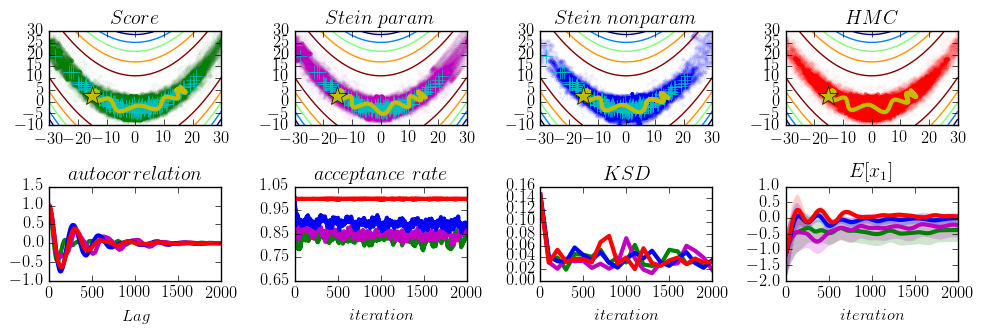
\includegraphics[width=1.0\linewidth]{figs/banana.png}
\vspace{-0.2in}
\caption{Kernel induced Hamiltonian flow compared with HMC. Top: samples generated from the dynamics, training data (in cyan), an the trajectory of a particle for $T=1$ to $200$ starting at the star location (in yellow). Bottom: statistics computed during simulations. See main text for details.}
\vspace{-0.1in}
\label{fig:banana_example}
\end{figure}

\subsection{Meta-learning of approximate posterior samplers for Bayesian NNs}
\label{sec:chap6_meta}
%
One of the recent focuses on meta-learning has been on learning optimisers for training deep neural networks, e.g.~see \cite{andrychowicz:gradient2016, li:optimize2016}. Could analogous goals be achieved for approximate inference? In this section we attempt to learn an approximate posterior sampler for Bayesian neural networks (Bayesian NNs, BNNs) that generalises to \emph{unseen} datasets and architectures, and we refer to Section \ref{sec:chap5_wild_applications} for a motivation of this approach. 

In a nutshell, we consider a binary classification task: $p(y = 1|\x, \mparam) = \text{sigmoid}(\text{NN}_{\mparam}(\x))$, $p_0(\mparam) = \mathcal{N}(\mparam; \bm{0}, \mathbf{I})$. After observing the training data $\data = \{(\x_n, y_n)\}_{n=1}^N$, we first obtain the approximate posterior $q_{\vparam}(\mparam) \approx p(\mparam | \data) \propto p_0(\mparam) \prod_{n=1}^N p(y_n | \x_n, \mparam)$, then approximate the predictive distribution for a new observation as $ p(y^*=1|\x^*, \data) \approx \frac{1}{K} \sum_{k=1}^K p(y^*=1|\x^*, \mparam^k), \mparam^k \sim q_{\vparam}(\mparam). $ 
%
In this task we define an implicit approximate posterior distribution $q_{\vparam}(\mparam)$ as the following \emph{stochastic} RNN $\mparam_{t+1} = \f(\mparam_t, \nabla_t, \bm{\epsilon}_t)$: given the current location $\mparam_t$ and the mini-batch data $\{ (\x_m, y_m) \}_{m=1}^M$, the update for the next step is
\begin{equation}
\begin{aligned}
\mparam_{t+1} &= \mparam_{t} + \zeta \Delta_{\vparam}(\mparam_t, \nabla_t) + \bm{\sigma}_{\vparam}(\mparam_t, \nabla_t) \odot \bm{\epsilon}_t, \quad \bm{\epsilon}_t \sim  \mathcal{N}(\bm{\epsilon}; \bm{0}, \mathbf{I}),\\
\nabla_t &= \nabla_{\mparam_t} \left[ \frac{N}{M} \sum_{m=1}^M \log p(y_m|\x_m, \mparam_t) + \log p_0(\mparam_t) \right] .
\end{aligned}
\end{equation}
The coordinates of the noise standard deviation $\bm{\sigma}_{\vparam}(\mparam_t, \nabla_t)$ and the moving direction $\Delta_{\vparam}(\mparam_t, \nabla_t)$ are parametrised by a \emph{coordinate-wise} neural network, i.e.~
$$\bm{\sigma}_{\vparam}(\mparam_t, \nabla_t) = [\bm{\sigma}_{\vparam}(\mparam_t(1), \nabla_t(1)), ..., \bm{\sigma}_{\vparam}(\mparam_t(d), \nabla_t(d)) ]^{\text{T}}$$
with $\mparam_t(i)$ denoting the $i^{\text{th}}$ dimension of vector $\mparam_t$ (similarly for $\nabla_t(i)$ and $\Delta_{\vparam}(\mparam_t, \nabla_t)$).
%
If properly trained, this neural network will learn the best combination of the current location and gradient information, and produce approximate posterior samples efficiently on different probabilistic modelling tasks.

We propose using the variational inference objective (\ref{eq:vi_objective_entropy}) computed on the samples $\{ \mparam_t^k \}$ to learn the variational parameters $\vparam$. 
%
More specifically, we simulate the approximate sampler for $T = 10$ transitions and sum over the variational lower-bounds computed on the samples of every step. This gives the maximisation objective
$$\mathcal{L}(\vparam) = \sum_{t=1}^T \mathcal{L}_{\text{VI}}(q_t),$$
with $q_t(\mparam)$ as the marginal distribution of $\mparam_t$ (therefore depends on $\vparam$). In practice the variational lower-bound $\mathcal{L}_{\text{VI}}(q_t)$ is further approximated by Monte Carlo and data sub-sampling:
$$ \mathcal{L}_{\text{VI}}(q_t) \approx \frac{N}{K M} \sum_{m = 1}^M \sum_{k=1}^K \log p(y_m|\x_m, \mparam_t^k) + \log p_0(\mparam_t^k) - \log q_t(\mparam_t^k).$$
%
Since in this case the gradient of the log joint distribution can be computed analytically, we only approximate the gradient of the entropy term $\mathbb{H}[q]$ as in (\ref{eq:entropy_gradient}), with the exact score function replaced by the presented gradient estimators. 

\begin{figure}[t]
\subfigure[SGLD]{
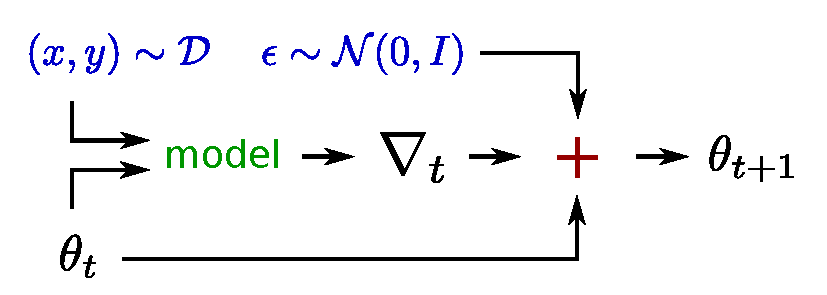
\includegraphics[width=0.45\linewidth]{figs/sgld_sampler.pdf}}
\hfill
\subfigure[NN-based approx.~sampler]{
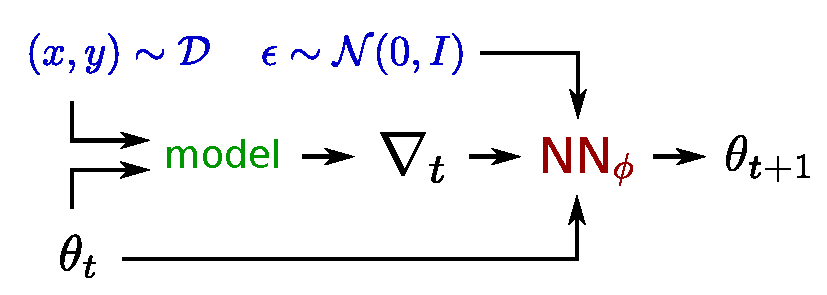
\includegraphics[width=0.45\linewidth]{figs/nn_sampler.pdf}}
\caption{Comparing the computation graphs of the two samplers. SGLD can be viewed as stochastic gradient descent plus properly scaled Gaussian noise. Instead of using the ``plus'' operation, the NN-based sampler combine the three inputs with a neural network, and the parameters $\vparam$ are then trained by the method described in the main text.}
\label{fig:sgld_nn_sampler_compare}
\end{figure}

We briefly describe the test protocol. We take from the UCI repository \citep{Lichman:uci_data2013} six binary classification datasets (australian, breast, crabs, ionosphere, pima, sonar), train an approximate sampler on crabs with a small neural network that has one 20-unit hidden layer with \emph{ReLU} activation, and generalise to the remaining datasets with a bigger network that has 50 hidden units and uses \emph{sigmoid} activation. We use ionosphere as the validation set to tune $\zeta$. The remaining 4 datasets are further split into 40\% training subset for simulating samples from the approximate sampler, and 60\% test subsets for evaluating the sampler's performance.
%
Besides the gradient estimators we also compare with two baselines: an approximate posterior sampler trained by maximum a posteriori (MAP), and stochastic gradient Langevin dynamics (SGLD) \citep{welling:sgld2011} evaluated on the test datasets directly. A comparison between SGLD and the proposed neural network based approximate sampler is visualised in Figure \ref{fig:sgld_nn_sampler_compare}. 

For architecture details, we use a one hidden layer neural network with 20 hidden units to compute the noise standard deviation $\bm{\sigma}_{\vparam}(\mparam_t, \nabla_t)$ and the moving direction $\Delta_{\vparam}(\mparam_t, \nabla_t)$ of the next update. Softplus non-linearity is used for the hidden layer and to compute the noise variance we apply ReLU activation to ensure non-negativity. The step-size $\zeta$ is selected as $10^{-5}$ which is tuned on the KDE approach. For SGLD step-size $10^{-5}$ also returns overall good results.\footnote{We note here that the results can be further improved with carefully tuned learning rate for both SGLD and the NN-based samplers, but here we are mainly interested in the same step-size set-up in order to compare the velocity of the particles defined by the underlying dynamics of the samplers.}
We report the results using the non-parametric Stein gradient estimator as we found it works better than the parametric version. The RBF kernel is applied for gradient estimation, with the hyper-parameters determined by a grid search on the bandwidth $\sigma^2 \in \{0.25, 1.0, 4.0, 10.0, \text{median trick} \}$ and $\eta \in \{0.1, 0.5, 1.0, 2.0\}$.

\begin{figure}[t]
\centering
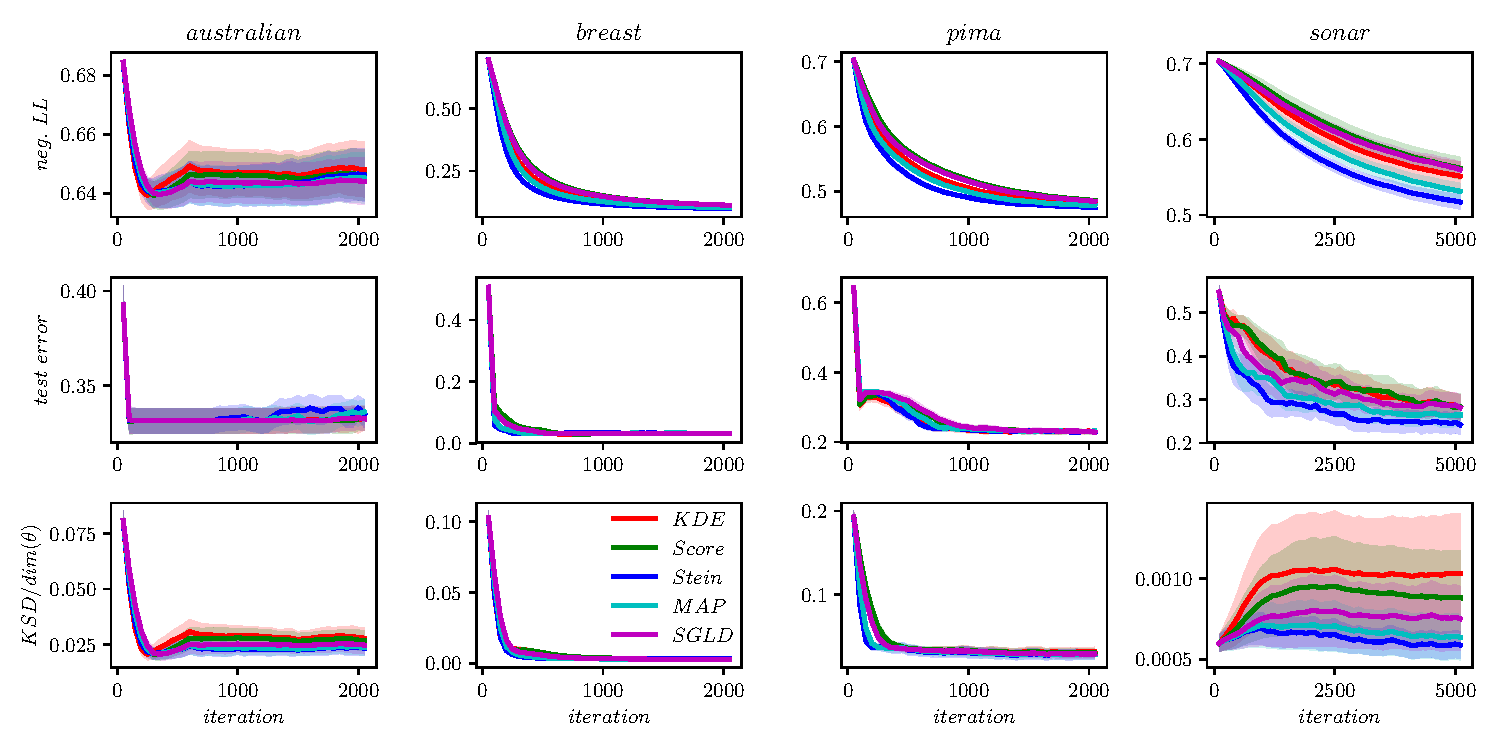
\includegraphics[width=1.0\linewidth]{figs/nn_sampler_results_new.pdf}
\vspace{-0.2in}
\caption{Generalisation performances for trained approximate posterior samplers.}
\vspace{-0.1in}
\label{fig:nn_sampler_results}
\end{figure}

Figure \ref{fig:nn_sampler_results} presents the (negative) test log-likelihood (LL), classification error, and an estimate of the KSD U-statistic $\mathcal{S}^2_U(p(\mparam | \D), q(\mparam))$ (with data sub-sampling) over 5 splits of each test dataset.\footnote{After conference publication (see publication page) I fixed a few issues of the previous implementation (mainly for the score matching estimator) and re-run the experiments, which is reported in this thesis.} 
%
The Stein approach performs equally well or a little better than SGLD in terms of test-LL and test error. The KDE method is slightly worse and is close to MAP, indicating that the KDE estimator does not provide a very informative gradient for the entropy term.
%
%The MAP model under-performs for test log-likelihood and KSD metrics, presumably because the noise variance $\bm{\sigma}$ has been turned off during learning thus having discovered an optimiser instead. 
%
The score matching estimator method produces the worst results among the trained samplers even after carefully tuning the bandwidth and the regularisation parameter $\eta$, although the difference is not significant. 
%
Future work should investigate the usage of advanced recurrent neural networks such as an LSTM \citep{hochreiter:lstm1997}, which is expected to return better performance.

\subsection{Towards addressing mode collapse in GANs using entropy regularisation}
GANs are notoriously difficult to train in practice. Besides the instability of gradient-based minimax optimisation which has been partially addressed by many recent proposals \citep{salimans:training2016, arjovsky:wgan2017, berthelot:began2017}, they also suffer from mode collapse. We propose adding an entropy regulariser to the GAN generator loss. Concretely, assume the generative model $p_{\mparam}(\x)$ is implicitly defined by $\x = \f_{\bm{\theta}}(\z), \z \sim p_0(\z)$, then the generator's loss is defined by 
\begin{equation}
\tilde{\mathcal{J}}_{\text{gen}}(\mparam) = \mathcal{J}_{\text{gen}}(\mparam) - \alpha \mathbb{H}[p_{\mparam}(\x)],
\label{eq:gan_regularised_general}
\end{equation}
where $\mathcal{J}_{\text{gen}}(\mparam)$ is the original loss function for the generator from any GAN algorithm and $\alpha$ is a hyper-parameter. In practice the gradient of (\ref{eq:gan_regularised_general}) is estimated using Monte Carlo.

As an illustrating example, in the following we consider the very recently proposed boundary equilibrium GAN (BEGAN) \citep{berthelot:began2017} approach. In BEGAN the discriminator is defined as an auto-encoder $D_{\hparam}(\x)$ that reconstructs the input $\x$. After selecting a ratio parameter $\gamma > 0$, a control rate $\beta_0$ initialised at 0, and a ``learning rate'' $\lambda > 0$ for the control rate, the loss functions for the generator $\x = \f_{\mparam}(\z), \z \sim p_0(\z)$ and the discriminator are:
\begin{equation}
\begin{aligned}
& \mathcal{J}(\x) =  || D_{\hparam}(\x) - \x ||, \quad || \cdot || = || \cdot ||_2^2 \text{ or } || \cdot ||_1, \\
& \mathcal{J}_{\text{gen}}(\mparam; \hparam) = \mathcal{J}(\f_{\mparam}(\z)), \quad \z \sim p_0(\z)  \\ 
& \mathcal{J}_{\text{dis}}(\hparam; \mparam) = \mathcal{J}(\x) - \beta_t \mathcal{J}_{\text{gen}}(\mparam; \hparam), \quad \x \sim \D \\
& \beta_{t+1} = \beta_t + \lambda (\gamma \mathcal{J}(\x) - \mathcal{J}(\f_{\mparam}(\z))).
\end{aligned}
\label{eq:began_original}
\end{equation}
The main idea behind BEGAN is that, as the reconstruction loss $\mathcal{J}(\cdot)$ is approximately Gaussian distributed, with $\gamma = 1$ the discriminator loss $\mathcal{J}_{\text{dis}}$ is (approximately) proportional to the Wasserstein distance between loss distributions induced by the data distribution $p_{\D}(\x)$ and the generator $p(\x)$. In practice it is beneficial to maintain the equilibrium $\gamma \mathbb{E}_{p_{\D}} \left[ \mathcal{J}(\x) \right] = \mathbb{E}_{p} \left[ \mathcal{J}(\x) \right] $ through the optimisation procedure described in (\ref{eq:began_original}) that is motivated by proportional control theory. This approach effectively stabilises training, however it suffers from catastrophic mode collapse problem (see the left most panel in Figure \ref{fig:gan_samples}). 

We empirically investigate the entropy regularisation idea on BEGAN using (continuous) MNIST. 
As described before, we simply subtract an entropy term from the generator's loss function, i.e. with $K$ samples $\z^1, ..., \z^k \sim p_0(\z)$,
\begin{equation}
\tilde{\mathcal{J}}_{\text{gen}}(\mparam; \hparam) = \frac{1}{K} \sum_{k=1}^K \mathcal{J}(\f_{\mparam}(\z^k)) + \alpha \frac{1}{K} \sum_{k=1}^K \log p(\f_{\mparam}(\z^k)),
\end{equation}
where the rest of the optimisation objectives remains as in (\ref{eq:began_original}). This procedure would maintain the equilibrium $\gamma \mathbb{E}_{p_{\D}} \left[ \mathcal{J}(\x) \right] = \mathbb{E}_{p} \left[ \mathcal{J}(\x) \right] - \alpha \mathbb{H}[p]$. We approximate the gradient $\nabla_{\mparam} \mathbb{H}[p]$ using the estimators presented above. For the purpose of updating the control rate $\beta_t$ two strategies are considered to approximate the contribution of the entropy term. The first proposal considers a plug-in estimate of the entropy term with a KDE estimate of $p(\x)$, which is consistent with the KDE estimator but not necessary with the other two (as they use kernels when representing $\log p(\x)$ or $\nabla_{\x} \log p(\x)$). The second one uses a proxy of the entropy loss $-\tilde{\mathbb{H}}[p] = \frac{1}{K} \sum_{k=1}^K \nabla_{\x^k} \log \hat{p}(\x^k)^{\text{T}} \x^k$ with $\nabla_{\x^k} \log \hat{p}(\x^k)$ is the approximate gradient obtained by the estimators. It is the surrogate loss used to (approximately) compute $\nabla_{\vparam} \mathbb{H}[p]$:
$$
\nabla_{\vparam} \mathbb{H}[p] \approx \nabla_{\vparam} \tilde{\mathbb{H}}[p] = \frac{1}{K} \sum_{k=1}^K \nabla_{\x^k} \log \hat{p}(\x^k)^{\text{T}} \nabla_{\vparam} \x^k.
$$

We compare the non-parametric V-statistic Stein gradient estimator to both KDE and score matching estimators. We use a convolutional generative network and a convolutional auto-encoder and select the hyper-parameters of BEGAN $\gamma \in \{0.3, 0.5, 0.7\}$, $\alpha \in [0, 1]$ and $\lambda = 0.001$. The Epanechnikov kernel $\mathcal{K}(\x, \x') := \frac{1}{d} \sum_{j=1}^d (1 - (x_j - x'_j)^2)$ is used as the pixel values lie in a unit interval (see Appendix \ref{sec:appendix_stein} for the expression of the score matching estimator), and to ensure the boundary condition we clip the pixel values into range $[10^{-8}, 1-10^{-8}]$. Readers are referred to Appendix \ref{sec:appendix_stein} for a detailed experimental set-up.

The generated images are visualised in Figure \ref{fig:gan_samples}. BEGAN without entropy regularisation fails to generate diverse samples even when trained with learning rate decay. The other three images clearly demonstrate the benefit of the entropy regularisation technique, with the Stein approach obtaining the highest diversity without compromising visual quality.

%
We further consider four metrics to assess the trained models quantitatively. First 500 samples are generated for each trained model, then we compute their nearest neighbours in the training set using $\ell_1$ distance, and obtain a probability vector $\mathbf{p}$ by averaging over these neighbour images' label vectors. In Figure \ref{fig:gan_results} we depict the entropy of $\mathbf{p}$  (top left), averaged $\ell_1$ distances to the nearest neighbour (top right), and the difference between the largest and smallest elements in $\mathbf{p}$ (bottom right). The error bars are obtained by 5 independent runs. These results demonstrate that the Stein approach performs significantly better than the other two, in that  it learns a better generative model not only faster but also in a more stable way. Interestingly the KDE approach achieves the lowest average $\ell_1$ distance to nearest neighbours, possibly because it tends to memorise training examples. We next train a fully connected network $\pi(\y|\x)$ on MNIST that achieves 98.16\% text accuracy, and compute on the generated images an empirical estimate of the inception score \citep{salimans:training2016} $\mathbb{E}_{p(\x)}[\mathrm{KL}[\pi(\y|\x) || \pi(\y)] ]$ with $\pi(\y) = \mathbb{E}_{p(\x)}[\pi(\y|\x)]$ (bottom left panel). High inception score indicates that the generate images tend to be both realistic looking and diverse, and again the Stein approach out-performs the others on this metric by a large margin. 

Concerning computation speed, all the three methods are of the same order: 10.20s/epoch for KDE, 10.85s/epoch for Score, and 10.30s/epoch for Stein.\footnote{All the methods are timed on a machine with an NVIDIA GeForce GTX TITAN X GPU.} This is because $K < d$ (in the experiments $K=100$ and $d=784$) so that the complexity terms are dominated by kernel computations ($\mathcal{O}(K^2 d)$) required by all the three methods. Also for a comparison, the original BEGAN method without entropy regularisation runs for 9.05s/epoch. Therefore the main computation cost is dominated by the optimisation of the discriminator/generator, and the proposed entropy regularisation can be applied to many GAN frameworks with little computational burden.

\begin{figure}[t]
\vspace{-0.2in}
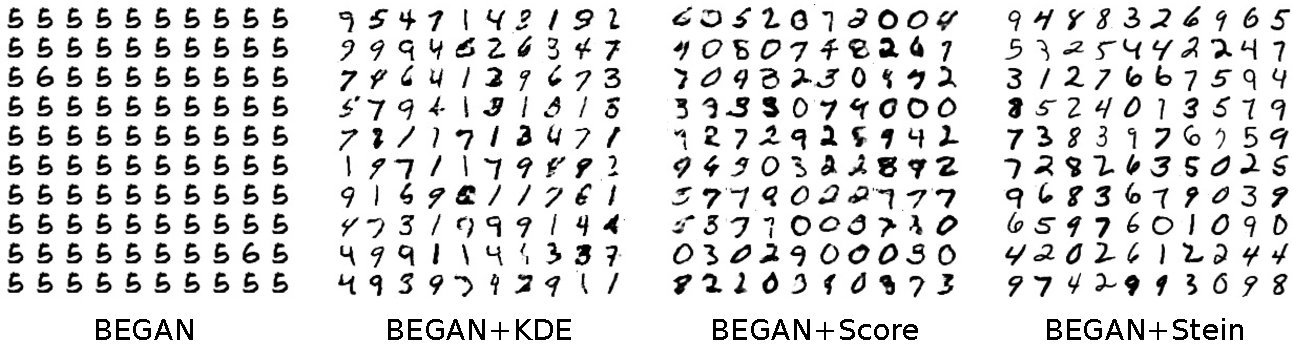
\includegraphics[width=1.0\linewidth]{figs/gan_samples.pdf}
\vspace{-0.2in}
\caption{Visualisation of generated images from trained BEGAN models.}
\label{fig:gan_samples}
\vspace{0.1in}
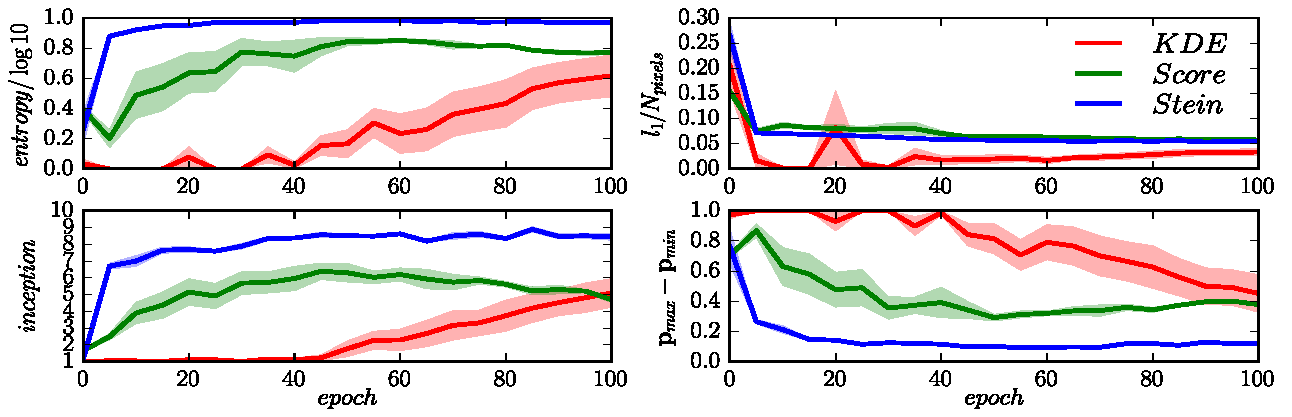
\includegraphics[width=1.0\linewidth]{figs/gan_results.pdf}
\vspace{-0.2in}
\caption{Quantitative evaluation on entropy regularised BEGAN. The higher the better for the LHS panels and the other way around for the RHS ones. See main text for details.}
\vspace{-0.1in}
\label{fig:gan_results}
\end{figure}

\section{Summary}
\label{sec:conclusions}

We have presented the Stein gradient estimator as a novel generalisation to the score matching gradient estimator. With a focus on learning implicit models, we have empirically demonstrated the efficacy of the proposed estimator by showing state-of-the-art results on three canonical learning tasks: approximating gradient-free MCMC, meta-learning for approximate posterior samplers, and unsupervised learning for image generation. Future work will expand the understanding of gradient estimators in both theoretical and practical sides. Theoretical development will compare both the V-statistic and U-statistic Stein gradient estimators. Practical work will improve the sample efficiency of kernel estimators in high dimensions and develop fast yet accurate approximations to the matrix inversion part. Finally follow-up work will study the generalisation of the Stein gradient estimator to non-kernel settings and discrete distributions.


\vspace{3em}
{\Large
\noindent \hrulefill \hspace{0.2cm} \raisebox{-4pt}[10pt][10pt]{\decofourleft ~  \decosix ~ \decofourright} \hspace{0.1cm} \hrulefill
\vspace{2em}
}

Here comes the end of the second theme of the thesis, where we have discussed principles of approximate inference algorithm design (Chapter \ref{chap:wild}) and presented one concrete example (Chapter \ref{chap:grad_approx}) on learning wild approximations. Readers might have noticed that wild approximate inference is still a very new research direction: many related papers in citation are freshly baked within a year of this thesis submission, and the proposals in development are inspired by recent success in machine learning and deep learning. Thus both theoretical analyses and extensive comparisons to traditional approaches are much in need, which will then help identify the ideal application scenarios and possibly potential pitfalls of the method.

The presented two themes have substantial differences. In the next chapter, which concludes the thesis, I will summarise the contributions of the thesis to the approximate inference community, and discuss the connections and comparisons between the two themes. Expositions of important research questions will also be provided, and hopefully this will serve as a principled guide for future development of approximate inference algorithms.
%\include{Chapter8/chapter8}
\chapter{Conclusions and Future Work}
\label{chap:conclusion}

% **************************** Define Graphics Path **************************
\ifpdf
    \graphicspath{{Chapter7/Figs/Raster/}{Chapter7/Figs/PDF/}{Chapter7/Figs/}}
\else
    \graphicspath{{Chapter7/Figs/Vector/}{Chapter7/Figs/}}
\fi


Approximate inference is a huge subject, which studies both the \emph{structure of the approximate distribution}, and the \emph{optimisation algorithms} used to fit them. The thesis has mainly investigated the latter part, presenting a number of new approximate inference algorithms and their applications to Bayesian deep learning tasks. A summary of the contributions is provided in Section \ref{sec:conclusion_compare}, where I will also discuss comparisons and connections between the two thesis themes. Much work is still required to enable generic $q$ distributions to be fitted accurately and efficiently, and in Section \ref{sec:conclusion_future} I will briefly provide my perspective on this matter, and raise several important questions to be answered in the future.
\section{More discussions on the two themes}
\label{sec:conclusion_compare}

Although the thesis mainly discussed new optimisation algorithms for approximate inference, the material was organised into two themes.
\begin{itemize}
\item[I] Unifying variational methods. (Chapters \ref{chap:background}, \ref{chap:factor_tying}, \ref{chap:vrbound}) \\
In this part of the thesis, we studied two main classes of variational algorithms, namely expectation propagation (EP) and variational inference (VI). The main contributions are the two novel frameworks: stochastic EP (Chapter \ref{chap:factor_tying}) and R{\'e}nyi divergence VI (Chapter \ref{chap:vrbound}). SEP significantly improves the memory efficiency of the EP-like algorithms, making them scalable to datasets comprising millions of instances. Extensions to the distributed SEP case further provide a highly flexible framework that unifies global and local approximation algorithms from an algorithmic perspective. Next we introduced the VR bound framework that enables the deployment of Monte Carlo methods for $\alpha$-divergence methods, provides both upper- and lower-bounds to the marginal likelihood, and again connects global and local approaches, but from an energy point of view.

\item[II] Wild approximate inference. (Chapters \ref{chap:wild}, \ref{chap:grad_approx}) \\
This theme presented a new research direction for approximate inference, with the goal of allowing \emph{arbitrarily} complex approximate posteriors to be deployed. In Chapter \ref{chap:wild}, I argued that the density evaluation requirement should be removed when designing Monte Carlo based approximate inference algorithms. I showed that this allows the use of very flexible $q$ distributions, and presented several examples of them. Later I wrote a generic guide for these designs, containing four different algorithmic options. One of the schemes (direct gradient approximation) was further developed in Chapter \ref{chap:grad_approx}, in which an initial experiment on meta-learning for approximate inference was presented.
\end{itemize}

The two themes were motivated in very different ways. The study of the unified frameworks aimed at developing new algorithms that both advance the understanding of existing variational methods, and adapt well to the application areas for Bayesian deep learning. All the discussions and comparisons in that part were based on one assumption: the candidate approximate distribution family $\mathcal{Q}$ is pre-defined, such as mean-field Gaussians. Indeed in the empirical studies we used implementations of almost the same set-up, except that we tuned a few of the algorithmic settings such as the $\alpha$ values and the number of MC samples $K$.

Wild approximate inference, on the other hand, encourages the use of very complex approximate distributions. There is no reason to expect an accurate approximation with a distribution that factorises in general, even when it is fitted using algorithms with elegant theoretical properties (like VI/EP studied in the first theme). However, instead of providing recipes for complex approximate distribution designs (see some recent examples in Appendix \ref{chap:optional}) which fit the existing algorithms, we made a bold move to developing algorithms that enable approximations of arbitrary form. By doing this, we allow the users to focus on the \emph{statistical properties} that they want to plant into the approximations, rather than the \emph{algorithmic tractability} aspects that restrict the flexibility of the $q$ distribution. 

Considering hyper-parameter optimisation, there is another notable difference between the two themes. For the first theme, we designed energy functions to allow training both the hyper-parameters and the $q$ distribution, where as for the second theme, we decoupled the algorithms for inference and learning.\footnote{Although for example the approximate maximum likelihood procedure does not require the inference optimisation to converge.} In this way, wild approximate inference is more in line with numerical integration methods like quadrature and Monte Carlo: all of them treat (approximate) Bayesian inference as a \emph{computational} task, and leave the learning procedure to hyper-parameter optimisation and potentially model selection. However, when compared to the VAE approach, it becomes harder to understand the interaction between the approximate inference results and the hyper-parameter updates. In this regard, the VR bound framework might be preferred, as both procedures are coupled, and can be analysed by examining the single loss function in use. We will continue the discussion on this matter in the next section.


Nevertheless, there is one important technique that has repeatedly been discussed in both themes: the Monte Carlo approximation method. It has been crucial to the recent success of Bayesian deep learning \citep{graves:practical2011, kingma:vae2014, rezende:vae2014, blundell:bnn2015, gal:uncertainty2016, li:amcmc2017}, as for deep neural networks most of the quantities that a Bayesian would like to compute are analytically intractable, even when using approximate posterior distributions with simple forms. In this thesis, except for SEP, the MC approximation is applied to all the other algorithms when performing empirical evaluations. Even SEP is compatible with Monte Carlo methods: when the moment matching step has no analytical solution, Monte Carlo methods can be deployed to estimate the sufficient statistics of the tilted distribution that are required for the update \citep{barthelme:abc2011, gelman:dep2014}. 


\section{Open problems}
\label{sec:conclusion_future}

Arguably, approximate inference is the key subject for research in Bayesian deep learning and large-scale Bayesian modelling in general. Therefore it is important to identify the challenges and open questions for future investigation. The final section of the thesis is organised in three parts. In the first two subsections, I discuss open research problems for the two themes. Then in the end, I ask the final question on the relationship between approximate inference and Bayesian modelling. 

\subsection{Research challenges for EP-like methods}
\paragraph{Is SEP guaranteed to converge? \\}
One can study the energy functions and prove that R{\'e}nyi divergence VI and BB-$\alpha$ methods are guaranteed to converge under mild conditions. However, since the development in 2015, little progress has been made to find the energy (or Lyapunov) function of SEP. One important research direction is to identify the existence of this energy function. On the other hand, \citet{dehaene:aep2015, dehaene:aep2018} used the AEP (the batch version of SEP) to study the convergence of EP without looking at an energy function. Although having assumed some restrictive conditions for simplicity, the proof ideas in \citet{dehaene:aep2015, dehaene:aep2018} can still be useful for future research. 

\paragraph{More theoretical supports on selecting the $\alpha$-divergence? \\}
We have conjectured the behaviour of the $\alpha$-divergence methods using both toy examples (see Section \ref{sec:chap4_mean_field}) and empirical results. However, there exists no formal theory so far which support (or disprove) these hypotheses. Furthermore, most of these intuitions apply to uni-modal approximations, and it is still largely unknown how the approximation methods perform when multi-modal distributions are fitted using $\alpha$-divergence methods. Perhaps proving theoretical results for the general set-up might be hard, so a sensible plan would first propose theorems on toy problems, and also design (counter) examples that (dis)agree with the intuitions provided in this thesis. Also algorithmic design for automatic divergence selection would be much welcomed, in this regard, one can use Bayesian optimisation methods \citep{movckus:bo1975, snoek:bo2012}, or design an objective function to learn the $\alpha$ values \citep{dikmen:divergence2015}.

\paragraph{Generalisation results for future observations? \\}
In many applications of Bayesian deep learning, the predictive performances are mainly the focus of the model evaluation. Variational inference might be preferred in this regard, as under some assumptions, the PAC-Bayes framework provides generalisation bounds on future observations (coming from the same underlying distribution as the training data) that are directly related to the variational free-energy \citep{mcallester:pac1998, germain:pac2016}. Preliminary results showed that some generalisation bounds of other forms could also be proved using R{\'e}nyi divergences \citep{begin:pac2016}, however it is unclear how this is related to the $\alpha$-divergence framework studied in this thesis. Future research on this challenge would also advance the understanding of $\alpha$-divergence methods, therefore helping address the above question as well.


\subsection{Open challenges for wild approximate inference}
\paragraph{How do we design the approximate posterior? \\}
A good design for the approximate posterior is still very much in need, even when the wild approximate inference framework allows more flexible $q$ distributions to be fitted by relaxing the algorithmic tractability constraints. For example, the density ratio estimation method discussed in Section \ref{sec:chap5_wild_solutions} requires a rather significant number of MC samples, which can be very expensive when applied to mini-batch optimisations for latent variable models. One very interesting solution to this issue is by sharing the randomness across the inference procedure associated with different latent variables \citep{mescheder:avb2017}. Another important concern considers ``better compression of posterior correlation'', i.e.~how we can design the approximation to capture the correlation between variables with the least amount of computation and memory. This can be especially useful for Bayesian neural networks, and having the structural information of the posterior can significantly improve both predictive performance and uncertainty calibration. 

\paragraph{Variance reduction/control variate methods for wild approximate inference? \\}
With Monte Carlo approximations, the stochastic gradients used to update the $q$ distributions can be very noisy. Efforts have been made recently to reduce the variance of the gradient signal for the MC-VI method, including control variate approaches, see \citet{paisley:bbvi2012, mnih:nvil2014, gu:muprop2016}. We note that variance reduction has also been an important research direction for both reinforcement learning \citep{greensmith:rl_variance2004, gu:qprop2017} and stochastic optimisation \citep{leroux:sag2012, johnson:svrg2013, defazio:saga2014}.\footnote{Three NIPS 2016 tutorials -- on VI, deep RL and stochastic optimisation, respectively -- had spent a considerate amount of time discussing variance reduction.} It might be helpful to borrow ideas from those fields to develop control variate methods for wild approximate inference.

\paragraph{Wild approximate inference methods for discrete latent variables?\\}
One of the imperfections of this thesis is that we did not discuss approximating posterior distributions for discrete variables. In this case the path derivative (i.e.~differentiation through an MC sample) is not available, and traditional VI has resorted to the REINFORCE gradient \citep{williams:reinforce1992}, potentially with control variate methods \citep{mnih:nvil2014, titsias:local_expectation2015, gu:muprop2016, mnih:vimco2016}. However, many of these methods still rely on a tractable $q$ density (or at least the tractability of the score function), which is not applicable in the wild approximate inference set-up. Some ad-hoc solutions include 1) a continuous relaxation of the discrete density, such as the Concrete distribution \citep{maddison:concrete2017, jang:gumble2017} which has some successful applications \citep{kusner:gan_gumbel2016, gal:concrete2017}; 2) weak derivatives or Stein discrepancies defined on discrete distributions, e.g.~see \citet{ranganath:ovi2016}.

\paragraph{Principled approaches towards meta-learning for approximate inference?\\}
We briefly discussed the research direction of meta-learning for approximate inference algorithms in Section \ref{sec:chap5_wild_applications}, with an initial attempt also presented in Section \ref{sec:chap6_meta}. Another interesting approach would consider learning \emph{variational objectives} for fitting the posterior distributions, i.e. the algorithm is defined by
\begin{equation}
\mathcal{A}_{\vparam}(p_n(\z_n)) = \argmax_{q \in Q} \ \mathcal{L}_{\vparam}(p_n(\z_n), q(\z_n)),
\end{equation}
and the parameters $\vparam$ are learned by optimising a meta-objective $\mathcal{L}_{\text{meta}}$ on $\mathcal{A}_{f_{\vparam}}(p_n(\z_n))$ for all $n = 1, ..., N$. However there exists no principled guide for the construction of such meta-objective in order to learn a superior algorithm. It might be useful to consider some desirable properties that one would like to incorporate. For example we might want: 1) reduced bias when $\mathcal{L}_{\vparam}$ is used as a surrogate for maximum likelihood, see \citet{turner:two_problems2011}; 2) reduced variance when Monte Carlo is deployed in the algorithm $\mathcal{A}_{\vparam}$. The former property can be achieved by learning a lower-bound $\mathcal{L}_{\vparam}$ to the log marginal likelihood that is (approximately) equally tight everywhere (c.f. Section \ref{sec:chap4_mean_field}), and for the latter, one might consider learning transferable control variates across different densities.


\subsection{Approximate inference as computation, or modelling?}

Conceptually, Bayesian inference is easy: one just needs to specify a model (including a prior distribution and a likelihood function), and later use a posterior distribution to study the unknown factors and quantify uncertainty given the observations. In particular, as a natural result of Bayes' rule, the posterior distribution is completely determined by the model and the observations. Therefore traditionally, exact posterior evaluation has been regarded as a \emph{computational} task: no more assumptions are required, and the only thing left is to proceed the computation of Bayes' rule. Model selection can also be performed using the Bayes factor for example, or even frequentist style hypothesis tests on the ``predictive model'' $p(\x^* | \data) = \int p(\x^* | \mparam) p(\mparam | \data) d \mparam$. Both of them can be computed easily if assuming exact inference is available.

Practically, however, Bayesian inference is hard: for most useful models in the real world, it is impractical to compute the exact posterior unless we have an unlimited amount of computational resources. Fortunately, we now have many efficient approximate inference algorithms, some of them approximate the computation of the posterior, and some of them directly approximate the predictive distribution. All of them are motivated as providing an accurate approximation to the Bayesian inference procedure, therefore at first glance, they should follow the philosophy of exact inference and be treated as a computation task as well. From this perspective, researchers are encouraged to develop new algorithms that focus on improving the approximation accuracy and running speed, and discovering better designs of the $q$ distribution to reduce the biases further.

On the other hand, the Bayesian decision process relies on the inference results which can only be performed approximately in practice. Critically, as long as we are proposing approximations, we are making further assumptions about the inference procedure and thus to the whole (approximate) decision making process! In this sense, we should also add the inference procedure to the decision, or \emph{predictive modelling} procedure. Here is a simple example in favour of this claim: consider a model whose posterior distribution is a truncated Gaussian. Then VI with a Gaussian approximation returns terrible approximations (because the zero-forcing property of VI would force the $q$ distribution to be a Dirac delta function), and based on this approximate inference result, the later model checking process can reject this under-performing ``approximate Bayesian prediction model'' even when the original model with exact inference is well behaved. We can potentially identify this false rejection of the model (in the usual Bayesian sense) by changing the approximation algorithm to EP, or the $q$ distribution to allow a non-smooth density. Indeed this view has also been discussed in e.g.~\cite{dawid:prequential1984, meng:posterior_pvalue1994, gelman:posterior_predictive1996, gelman:philosophy2013} which adds a bit of frequentist flavour to the predictive model selection procedure. 

What is the take home message from this interpretation? Besides the encouragement of developing better approaches to improve the inference procedure (which is the same call as from the perspective of computation), an interesting direction is to understand the bias of existing inference methods. With a better understanding of how these biases might interact with downstream decision making tasks, we can then carefully select the best inference method to achieves a desirable ``predictive model''.
%
For example, VI is known for penalising complicated models (if the prior prefers the simple ones) \citep{hinton:mdl1993}. Therefore, we can design specific types of the approximate posterior (e.g.~Gaussian dropout \citep{srivastava:dropout2014, kingma:variational_dropout2015}) to further sparsify Bayesian neural networks without compromising the predictive accuracy \citep{molchanov:variational_dropout2017, louizos:bayesian_compression2017}.

Finally, just to be clear: both views of approximate inference are useful for discovering new research directions that are generally beneficial to enrich the literature. For example, they can be used to propose criteria for evaluating an approximate inference procedure, and derive new principles for algorithmic design. I hope that, by investigating this problem, the community can draw inspiration from both views, and obtain a better understanding of the roles of approximate inference for modern Bayesian analysis.




% ********************************** Back Matter *******************************
% Backmatter should be commented out, if you are using appendices after References
%\backmatter

% ********************************** Bibliography ******************************
\begin{spacing}{0.9}

% To use the conventional natbib style referencing
% Bibliography style previews: http://nodonn.tipido.net/bibstyle.php
% Reference styles: http://sites.stat.psu.edu/~surajit/present/bib.htm

%\bibliographystyle{apalike}
%\bibliographystyle{unsrt} % Use for unsorted references 
\bibliographystyle{apalike} % use this to have URLs listed in References
\cleardoublepage
\bibliography{References/references} % Path to your References.bib file


% If you would like to use BibLaTeX for your references, pass `custombib' as
% an option in the document class. The location of 'reference.bib' should be
% specified in the preamble.tex file in the custombib section.
% Comment out the lines related to natbib above and uncomment the following line.

%\printbibliography[heading=bibintoc, title={References}]


\end{spacing}

% ********************************** Appendices ********************************

\begin{appendices} % Using appendices environment for more functunality

% ******************************* Thesis Appendix B ********************************

\chapter{Proofs and Derivations}
\label{chap:proofs}

\section{Derivations of PBP in Chapter \ref{chap:factor_tying}}
\label{sec:appendix_pbp}

We briefly describe the approximation techniques used in probabilistic back-propagation (PBP) for training Bayesian neural networks \citep{hernandez-lobato:pbp2015}. In this case the model is the following:
\begin{equation}
\centering
\begin{aligned}
p(\y_n| \x_n, W, \gamma) = \mathcal{N}(\y_n; \text{NN}_{W}(\x_b), \gamma^{-1}), \quad
p(W | \lambda) = \prod_{i, j, l} \mathcal{N}(W_{ij}^l; 0, \lambda^{-1}), \\ 
p(\lambda) = \text{Gamma}(\lambda; \alpha_0^{\lambda}, \beta_0^{\lambda}), \quad p(\gamma) = \text{Gamma}(\gamma; \alpha_0^{\gamma}, \beta_0^{\gamma}),
\end{aligned}
\end{equation}
where $\alpha_0^{\lambda}, \beta_0^{\lambda}, \alpha_0^{\gamma}, \beta_0^{\gamma}$ are prior parameters that are all set to 6.
%
We are interested in computing the approximate posterior of the following form:
\begin{equation}
q(W, \gamma, \lambda) = \prod_{i, j, l} \mathcal{N}(W_{ij}^l ; \mu_{ij}^l, v_{ij}^l) \text{Gamma}(\lambda; \alpha^{\lambda}, \beta^{\lambda}) \text{Gamma}(\gamma; \alpha^{\gamma}, \beta^{\gamma}),
\end{equation}
which is iteratively solved by EP. Since the moments of the random variables can also be obtained by differentiating through the (log) normalising constant of the tilted distribution $\log Z$, PBP first approximately computes the normalising constant by
\begin{equation}
\begin{aligned}
Z &= \int p(\y| \x, W, \gamma) q(W, \gamma, \lambda) dW d\gamma d\lambda \\
&\approx \int \mathcal{N}(\y ; \z_L, \gamma^{-1}) \mathcal{N}(\z_L | \bm{m}_{L}, \bm{v}_{L}) \text{Gamma}(\gamma; \alpha^{\gamma}, \beta^{\gamma}) d\z_L d\gamma \quad \text{// PBP forward pass} \\
&= \int \mathcal{T}(\y ; \z_L, \beta^{\gamma} / \alpha^{\gamma}, 2 \alpha^{\gamma}) \mathcal{N}(\z_L | \bm{m}_{L}, \bm{v}_{L}) d\z_L \quad \text{// student-t distribution} \\
&\approx \mathcal{N}(\y; \bm{m}_{L}, \beta^{\gamma} / (\alpha^{\gamma} - 1) + \bm{v}_L). \quad \text{// Gaussian approx.}
\end{aligned}
\end{equation}
%
It remains to specify the forward pass of PBP which approximate $\text{NN}_W(\x), W \sim q(W)$ by $\z_L \sim \mathcal{N}(\z_L | \bm{m}_{L}, \bm{v}_{L})$. A short summary of the idea is the following. Assume the inputs $\z_{l-1}$ to the $l^{\text{th}}$ layer are Gaussian distributed: $\z_{l-1} \sim \mathcal{N}(\z_{l-1} | \bm{m}_{l-1}, \bm{v}_{l-1})$, then when the network is wide, due to the central limit theorem the pre-activation $\bm{a}_l = W \z_{l-1} / \sqrt{\text{dim}(\z_{l-1})}$ is approximately Gaussian distributed with mean and variance determined by the means and variances of $\z_{l-1}$ and $W^l$. If the activation function is ReLU, then the distribution of $\z_l$ is a mixture of delta mass $\delta(\z_l = \bm{0})$ and truncated Gaussian at zero. The last step approximates this mixture distribution with a Gaussian distribution that matches the mean and variance, which leads to $\mathcal{N}(\z_l | \bm{m}_l, \bm{v}_l)$ that is used in later forward pass. We refer to \cite{hernandez-lobato:pbp2015} for the detailed derivation of $\bm{m}_l$ and $\bm{v}_l$. 

In the SEP experiments for PBP the update equations are almost the same, except that $Z$ is computed using the cavity distribution $q_{-1}(W, \gamma, \lambda) \propto p(W|\lambda) p(\lambda) p(\gamma) f(W)^{N-1} f(\gamma)^{N-1} f(\lambda)$.

\section{Proofs of theorems in Chapter \ref{chap:vrbound}}
\label{sec:appendix_proof_chap4}

\subsection{Proof of Theorem \ref{thm:chap4_vrbound_sampling_bound}}

%%%%%%% proof %%%%%%%%%
\begin{proof}
 1) First we prove for $\alpha \leq 1$, $\mathbb{E}_{\{ \bm{h}_k \} }[\hat{\mathcal{L}}_{\alpha, K}]$ is non-decreasing in $K$. It is straight forward to show the results holds for $\alpha=1$. We follow the proof in \cite{burda:iwae2016} for fixed $\alpha < 1$. Let $K > 1$ and the subset of indices $I = \{i_1, ..., i_{K'} \} \subset \{1, ..., K\}, K' < K$ randomly sampled from integers 1 to $K$. Then for any $\alpha < 1$:
 \begin{equation*}
 \begin{aligned}
  \mathbb{E}_{\{ \bm{h}_k \}_{k=1}^K }[\hat{\mathcal{L}}_{\alpha, K}] 
  &= \frac{1}{1 - \alpha} \mathbb{E}_{\{ \bm{h}_k \}} \left[ \log \frac{1}{K} \sum_{k=1}^K \left( \frac{p(\bm{h}_k, \bm{x})}{q(\bm{h}_k|\bm{x})}  \right)^{1 - \alpha} \right] \\
  &= \frac{1}{1 - \alpha} \mathbb{E}_{\{ \bm{h}_k \}} \left[ \log \mathbb{E}_{I \subset \{1, ..., K\}} \left[ \frac{1}{K'} \sum_{k=1}^{K'} \left( \frac{p(\bm{h}_{i_k}, \bm{x})}{q(\bm{h}_{i_k})}  \right)^{1 - \alpha} \right] \right] \\
  &\geq \frac{1}{1 - \alpha} \mathbb{E}_{\{ \bm{h}_k \}} \left[ \mathbb{E}_{I \subset \{1, ..., K\}} \left[ \log \frac{1}{K'} \sum_{k=1}^{K'} \left( \frac{p(\bm{h}_{i_k}, \bm{x})}{q(\bm{h}_{i_k})}  \right)^{1 - \alpha} \right] \right] \quad \text{($\log x$ is concave)}\\
  &= \frac{1}{1 - \alpha} \mathbb{E}_{\{ \bm{h}_k \}} \left[ \log \frac{1}{K'} \sum_{k=1}^{K'} \left( \frac{p(\bm{h}_k, \bm{x})}{q(\bm{h}_k|\bm{x})}  \right)^{1 - \alpha} \right] 
  = \mathbb{E}_{\{ \bm{h}_k \}_{k=1}^{K'} }[\hat{\mathcal{L}}_{\alpha, K'}] 
 \end{aligned}
 \end{equation*}
We used Jensen's inequality of logarithm for the lower-bounding result here. When $\alpha > 1$ we can proof similar result but with inequality reversed, simply because now $1 - \alpha < 0$. \\

2) Next we prove that, when $K \rightarrow \infty$ and $|\mathcal{L}_{\alpha}| < +\infty$, we have $\mathbb{E}_{\{ \bm{h}_k \}_{k=1}^K }[\hat{\mathcal{L}}_{\alpha, K}] \rightarrow \mathcal{L}_{\alpha}$ if $\hat{\mathcal{L}}_{\alpha, K}$ is absolutely integrable wrt.~$qd\mu = dQ$ for all $K \geq 1$ (in other words $\mathbb{E}_{\{ \bm{h}_k \}_{k=1}^K }[|\hat{\mathcal{L}}_{\alpha, K}|] < +\infty$). We only prove it for $\alpha \leq 1$, and for $\alpha > 1$ it can be proved in a similar way. First we use Jensen's inequality again for all finite $K$:
\begin{equation*}
 \begin{aligned}
  \mathbb{E}_{\{ \bm{h}_k \}_{k=1}^K }[\hat{\mathcal{L}}_{\alpha, K}] 
  &= \frac{1}{1 - \alpha} \mathbb{E}_{\{ \bm{h}_k \}} \left[ \log \frac{1}{K} \sum_{k=1}^K \left( \frac{p(\bm{h}_k, \bm{x})}{q(\bm{h}_k|\bm{x})}  \right)^{1 - \alpha} \right] \\
  &\leq \frac{1}{1 - \alpha} \log \mathbb{E}_{\{ \bm{h}_k \}} \left[ \frac{1}{K} \sum_{k=1}^K \left( \frac{p(\bm{h}_k, \bm{x})}{q(\bm{h}_k|\bm{x})}  \right)^{1 - \alpha} \right] = \mathcal{L}_{\alpha}.
 \end{aligned}
\end{equation*}
This implies $\limsup_{K \rightarrow +\infty} \mathbb{E}_{\{ \bm{h}_k \}_{k=1}^K }[\hat{\mathcal{L}}_{\alpha, K}] \leq \mathcal{L}_{\alpha}$. 

Then as an intermediate result we prove $\hat{\mathcal{L}}_{\alpha, K} \rightarrow \mathcal{L}_{\alpha}$ almost surely when $K \rightarrow \infty$. For $\alpha \neq 1$, since function $\log $ is continuous we again swap the limit and logarithm:
\begin{equation*}
\lim_{K \rightarrow +\infty} \frac{1}{1 - \alpha} \log \frac{1}{K} \sum_{k=1}^K \left( \frac{p(\bm{h}_k, \bm{x})}{q(\bm{h}_k|\bm{x})}  \right)^{1 - \alpha}  
=  \frac{1}{1 - \alpha} \log \lim_{K \rightarrow +\infty} \frac{1}{K} \sum_{k=1}^K \left( \frac{p(\bm{h}_k, \bm{x})}{q(\bm{h}_k|\bm{x})}  \right)^{1 - \alpha} .
\end{equation*}
Now since we assume $|\mathcal{L}_{\alpha}| < +\infty$, this implies $\mathbb{E}_{q} \left[ \left( \frac{p(\bm{h}, \bm{x})}{q(\bm{h}|\bm{x})} \right)^{1 - \alpha} \right]$ is finite. Also notice for all $\alpha$ values the ratio $p/q$ is non-negative. Thus by the strong law of large numbers we have
\begin{equation*}
\lim_{K \rightarrow +\infty} \frac{1}{K} \sum_{k=1}^K \left( \frac{p(\bm{h}_k, \bm{x})}{q(\bm{h}_k|\bm{x})}  \right)^{1 - \alpha} = \mathbb{E}_{q(\bm{h}|\bm{x})} \left[ \left( \frac{p(\bm{h}, \bm{x})}{q(\bm{h}|\bm{x})} \right)^{1 - \alpha} \right] \text{ a.~s.,}
\end{equation*}
%
then $\hat{\mathcal{L}}_{\alpha, K} \rightarrow \mathcal{L}_{\alpha}$ almost surely as $K \rightarrow +\infty$. When $\alpha = 1$ we can use similar method to prove $\lim_{K \rightarrow +\infty} \hat{\mathcal{L}}_{1, K} = \mathcal{L}_{\text{VI}}$ almost surely.

Finally, using the non-increasing in $\alpha$ result we will prove later we have $\hat{\mathcal{L}}_{\alpha, K} \geq \hat{\mathcal{L}}_{1, K}$. Thus we can apply Fatou's Lemma and obtain the following almost surely (notice $\mathbb{E}[\hat{\mathcal{L}}_{1, K}] = \mathcal{L}_{\text{VI}}$ for all $K$):
%
\begin{equation*}
\begin{aligned}
\mathcal{L}_{\alpha} - \mathcal{L}_{\text{VI}} &= \mathbb{E}[ \lim_{K \rightarrow +\infty} \hat{\mathcal{L}}_{\alpha, K} - \hat{\mathcal{L}}_{1, K}] \\
&\leq \liminf_{K \rightarrow +\infty} \mathbb{E}_{\{ \bm{h}_k \}_{k=1}^K }[\hat{\mathcal{L}}_{\alpha, K} - \hat{\mathcal{L}}_{1, K}] \\
&= \liminf_{K \rightarrow +\infty} \mathbb{E}_{\{ \bm{h}_k \}_{k=1}^K }[\hat{\mathcal{L}}_{\alpha, K}] - \mathcal{L}_{\text{VI}}.
\end{aligned}
\end{equation*}
%
Combining with the supremum bound, we have $\mathbb{E}_{\{ \bm{h}_k \}_{k=1}^K }[\hat{\mathcal{L}}_{\alpha, K}] \rightarrow \mathcal{L}_{\alpha}$ when $K$ goes to infinity. For $\alpha > 1$ we use Jensen's inequality to bound the limit infimum and the non-increasing property in $\alpha$ to bound the limit supremum. Thus the convergence result holds for all $\alpha \in \{\alpha: |\mathcal{L}_{\alpha}| < +\infty \}$.\\
%

3) $\mathbb{E}[\hat{\mathcal{L}}_{\alpha, K}]$ is non-increasing in $\alpha$: since expectation preserves monotonicity, it is sufficient to prove the result for $\hat{\mathcal{L}}_{\alpha, K}$. This can be proved in similar way as Theorem 3 and 39 in \cite{van_erven:renyi2014}, and we include the prove here for completeness. Notice that for $\alpha < \beta$ function $x^{\frac{1 - \alpha}{1 - \beta}}$ defined on $x > 0$ is convex when $\alpha < 1$ and concave when $\alpha > 1$. So applying Jensen's inequality:
\begin{equation*}
\begin{aligned}
\hat{\mathcal{L}}_{\alpha, K} = \frac{1}{1 - \alpha} \log \frac{1}{K} \sum_{k=1}^K \left( \frac{p(\bm{h}_k, \bm{x})}{q(\bm{h}_k|\bm{x})}  \right)^{1 - \alpha} 
&= \frac{1}{1 - \alpha} \log \frac{1}{K} \sum_{k=1}^K \left( \left( \frac{p(\bm{h}_k, \bm{x})}{q(\bm{h}_k|\bm{x})}  \right)^{1 - \beta} \right)^{\frac{1 - \alpha}{1 - \beta}} \\
&\geq \frac{1}{1 - \alpha} \log \left( \frac{1}{K} \sum_{k=1}^K \left( \frac{p(\bm{h}_k, \bm{x})}{q(\bm{h}_k|\bm{x})}  \right)^{1 - \beta} \right)^{\frac{1 - \alpha}{1 - \beta}} = \hat{\mathcal{L}}_{\beta, K}.
\end{aligned}
\end{equation*}

%
Continuity in $\alpha$: First we show $\hat{\mathcal{L}}_{\alpha, K}$ is continuous in $\alpha$ when $p(\bm{h}_k, \bm{x}) \neq 0$ for $\bm{h}_k \sim q$. For $\alpha \neq 0, 1, \infty$ and for any sequence $\{\alpha_n\} \rightarrow \alpha$ it is sufficient to show that
\begin{equation*}
\begin{aligned}
&\lim_{n \rightarrow \infty} \log \frac{1}{K} \sum_k q(\bm{h}_k|\bm{x})^{\alpha_n} p(\bm{h}_k, \bm{x})^{1 - \alpha_n} \\
=& \log \lim_{n \rightarrow \infty} \frac{1}{K} \sum_k q(\bm{h}_k|\bm{x})^{\alpha_n} p(\bm{h}_k, \bm{x})^{1 - \alpha_n} \quad \text{($\log x$ is a continuous function)} \\
=& \log \frac{1}{K} \sum_k \lim_{n \rightarrow \infty} q(\bm{h}_k|\bm{x})^{\alpha_n} p(\bm{h}_k, \bm{x})^{1 - \alpha_n} \quad \text{(finite sum)} \\
=& \log \frac{1}{K} \sum_k  q(\bm{h}_k|\bm{x}) \left( \frac{p(\bm{h}_k, \bm{x})}{q(\bm{h}_k|\bm{x})} \right)^{1 - \lim_{n \rightarrow \infty} \alpha_n} \quad \text{($a^x$ is continuous in $x$ for all $a > 0$)} \\
=& \log \frac{1}{K} \sum_k q(\bm{h}_k|\bm{x})^{\alpha} p(\bm{h}_k, \bm{x})^{1 - \alpha}.
\end{aligned}
\end{equation*}
We note that since we assume $\hat{\mathcal{L}}_{\alpha, K}$ is absolutely integrable, we have $p/q > 0$ almost everywhere on the support of $q$. Hence $\{ \hat{\mathcal{L}}_{\alpha_n, K} \}$ has point-wise limit $\hat{\mathcal{L}}_{\alpha, K}$ almost everywhere as $n \rightarrow +\infty$. 

For $\alpha = 0, 1, \infty$ the R{\'e}nyi divergence is defined by continuity so one can use the same technique to show the continuity of $\hat{\mathcal{L}}_{\alpha, K} $ on those $\alpha$ values for fixed $K$. Then since $\alpha_n \rightarrow \alpha$, for any $\epsilon > 0$, there exists $n$ that is large enough such that $\alpha_m \in (\alpha - \epsilon, \alpha + \epsilon)$ for all $m > n$. Using the monotonicity result, we have for $\forall m > n$, $\hat{\mathcal{L}}_{\alpha_m, K}$ is bounded in the interval $(\hat{\mathcal{L}}_{\alpha + \epsilon, K}, \hat{\mathcal{L}}_{\alpha - \epsilon, K})$ and by assumption we have $\mathbb{E}[ |\hat{\mathcal{L}}_{\alpha -\epsilon, K}|] < +\infty$ and $\mathbb{E}[ |\hat{\mathcal{L}}_{\alpha +\epsilon, K}|] < +\infty$. This allows us to apply the dominated convergence theorem to prove $\lim_{n \rightarrow +\infty} \mathbb{E}[\hat{\mathcal{L}}_{\alpha_n, K}] = \mathbb{E}[ \lim_{n \rightarrow +\infty} \hat{\mathcal{L}}_{\alpha_n, K}] = \mathbb{E}[ \hat{\mathcal{L}}_{\alpha, K}]$. Thus we have proved that $\mathbb{E}[ \hat{\mathcal{L}}_{\alpha, K}]$ is continuous on $\alpha \in \{ |\mathcal{L}_{\alpha}| < +\infty \}$ if $\hat{\mathcal{L}}_{\alpha, K}$ is absolutely integrable.

\end{proof}
%%%%%%%%%%%%%%%%%%%%%%%

\subsection{Proof of Corollary \ref{thm:chap4_vrbound_alpha_k_existence} }

The next question we are interested is that, given a fixed number of samples $K$, can we tune the $\alpha$ parameter to achieve the best approximation to the marginal likelihood? This is an important question as in practice only finite amount of computation resource is allowed. In the following we will discuss a corollary result based on Theorem \ref{thm:chap4_vrbound_sampling_bound}, but to prove it we first introduce the following lemmas. As we assume $\text{supp}(p) \subseteq \text{supp}(q)$, there might exist some regions that $q > 0$ but $p = 0$. We define $\rho = \int_{\text{supp}(q) \backslash \text{supp}(p)}dQ$ with $dQ = qd\mu$, and rewrite the computation of $\mathbb{E}[\hat{\mathcal{L}}_{\alpha, K}]$. The following lemma shows the importance of the absolute integrable assumption in Theorem \ref{thm:chap4_vrbound_sampling_bound}.

%%%%% lemma %%%%%

\begin{lemma}
Assume $\rho > 0$. Then for all finite $K$ and $\alpha < 0$, $\mathbb{E}_{\{\bm{h}_k\}_{k=1}^K} [ \hat{\mathcal{L}}_{\alpha, K}(q; \bm{x}) ] = -\infty$ and thus $\hat{\mathcal{L}}_{\alpha, K}$ is not integrable wrt.~$qd\mu = dQ$.
\label{lemma:chap4_vrbound_alpha_k_non_exist}
\end{lemma}

\begin{proof}
We define $\tilde{q}$ as the $q$ distribution restricted on the support of $p$, i.e.~$\tilde{q} = q / (1 - \rho)$ defined on $\text{supp}(p)$. Then for any fixed $K < +\infty$ and $\alpha < 0$, we have
\begin{equation*}
\begin{aligned}
\mathbb{E}_{\{\bm{h}_k\}_{k=1}^K \sim q} [ \hat{\mathcal{L}}_{\alpha, K}(q; \bm{x}) ] 
=& \rho^{K} \log 0 
+ \sum_{k=1}^K {K \choose k} \rho^{K - k} (1 - \rho)^{k} \left( \mathbb{E}_{\{\bm{h}_j\}_{j=1}^k \sim \tilde{q}}[\hat{\mathcal{L}}_{\alpha, k}(\tilde{q}; \bm{x})] + \frac{ \log k }{1 - \alpha} \right) \\
-& (1 - \rho^K) \left( \log (1 - \rho) + \frac{\log K}{1 - \alpha} \right) .
\end{aligned}
\end{equation*}
Thus $\mathbb{E}_{\{\bm{h}_k\}_{k=1}^K} [ \hat{\mathcal{L}}_{\alpha, K}(q; \bm{x}) ] = -\infty$ for all finite $K$ and $\alpha < 0$. 
\end{proof}

%%%%%%%%%%%%%%%%%%%%

The above example shows the pathology of MC approximation which is further discussed in Section \ref{sec:chap4_vrbound_opt_mc}. From now on we assume $\hat{\mathcal{L}}_{\alpha, K}$ is absolutely integrable w.r.t.~$dQ$ in order to apply Theorem \ref{thm:chap4_vrbound_sampling_bound}.

%%%%% lemma %%%%% 
 
\begin{lemma}
Assume $\alpha < 0$, $\hat{\mathcal{L}}_{\alpha, K}$ absolutely integrable wrt.~$qd\mu = dQ$ for all $K$, $\mathcal{L}_{\alpha} > \mathcal{L}_{\text{VI}}$, and $|\mathcal{L}_{\alpha}| < +\infty$. Then there exists $1 \leq K_{\alpha} < +\infty$ such that for all $K \leq K_{\alpha} < K'$, $\mathbb{E}_{\{\bm{h}_k\}_{k=1}^K} [ \hat{\mathcal{L}}_{\alpha, K}(q; \bm{x}) ] \leq \log p(\bm{x}) < \mathbb{E}_{\{\bm{h}_k\}_{k=1}^{K'}} [ \hat{\mathcal{L}}_{\alpha, K'}(q; \bm{x}) ]$. Also $K_{\alpha}$ is \textbf{non-decreasing} in $\alpha$ with $\lim_{\alpha \rightarrow 0} K_{\alpha} = + \infty$ and $\lim_{\alpha \rightarrow -\infty} K_{\alpha} \geq 1$.
\label{lemma:chap4_vrbound_alpha_k_existence}
\end{lemma}

\begin{proof}
%
1) Existence of $K_{\alpha}$: first from Theorem \ref{thm:chap4_vrbound_sampling_bound} we have $\mathbb{E}[\hat{\mathcal{L}}_{\alpha, K}]$ is non-decreasing in $K$ when $\alpha < 0$. Then since for all $\alpha$, $\mathbb{E}[\hat{\mathcal{L}}_{\alpha, 1}] = \mathcal{L}_{\text{VI}} \leq \log p(\bm{x})$, we have $K_{\alpha} \geq 1$ if $K_{\alpha}$ exists. Also from Theorem \ref{thm:chap4_vrbound_sampling_bound} we have $\lim_{K \rightarrow +\infty} \mathbb{E}[\hat{\mathcal{L}}_{\alpha, K}] = \mathcal{L}_{\alpha} > \log p(\bm{x})$ for all $\alpha < 0$. Hence for $\epsilon = \mathcal{L}_{\alpha} - \log p(\bm{x})$ there exist $K$ that is finite but large enough such that $\mathcal{L}_{\alpha} - \mathbb{E}[\hat{\mathcal{L}}_{\alpha, K'}] < \epsilon$ for all $K' > K$. Now we can define $\epsilon = \mathcal{L}_{\alpha} - \log p(\bm{x})$ and take $K_{\alpha}$ as the minimum of such $K$, and it is straight-forward to show that $1 \leq K_{\alpha} < +\infty$. 

%
2) $K_{\alpha}$ is non-decreasing in $\alpha$: suppose there exist $\alpha > \beta$ such that $K_{\alpha} < K_{\beta}$. Then there exist $K_{\alpha} < K \leq K_{\beta}$ such that $\mathbb{E}[\hat{\mathcal{L}}_{\alpha, K}] > \log p(\bm{x}) \geq \mathbb{E}[\hat{\mathcal{L}}_{\beta, K}]$. But Theorem \ref{thm:chap4_vrbound_sampling_bound} says $\mathbb{E}[\hat{\mathcal{L}}_{\alpha, K}]$ is non-increasing in $\alpha$, a contradiction. 

%
3) Since $\lim_{K \rightarrow +\infty} \mathbb{E}[\hat{\mathcal{L}}_{\alpha, K}] = \mathcal{L}_{\alpha}$ and $\mathcal{L}_{\alpha} \downarrow \log p(\bm{x})$ when $\alpha \uparrow 0$, we have $\lim_{\alpha \rightarrow 0} K_{\alpha} = +\infty$. Also since $K_{\alpha}$ is non-decreasing in $\alpha$ and is lower-bounded by 1, we have the limit exists and $\lim_{\alpha \rightarrow -\infty} K_{\alpha} \geq 1$.
\end{proof}

%%%%% end of lemma %%%%%

Now we prove Corollary \ref{thm:chap4_vrbound_alpha_k_existence} which answers the question of approximating the marginal likelihood with finite sample MC bound. 
It is sufficient to prove the corollary with the conditions assumed in Lemma \ref{lemma:chap4_vrbound_alpha_k_existence} since $K_{\alpha} = +\infty$ for the other cases, and if so for all $\alpha < 0$, then $\alpha_K = -\infty$ for all finite $K$.
\begin{proof}
 
1) Existence of $\alpha_K$ for $\lim_{\alpha \rightarrow -\infty} K_{\alpha} < K < +\infty$: from Lemma \ref{lemma:chap4_vrbound_alpha_k_existence} we can find $\alpha > \beta$ such that $K_{\alpha} \geq K \geq K_{\beta}$. This means  $\mathbb{E}[\hat{\mathcal{L}}_{\alpha, K}] \leq \log p(\bm{x}) \leq \mathbb{E}[\hat{\mathcal{L}}_{\beta, K}]$. Since $\mathbb{E}[\hat{\mathcal{L}}_{\alpha, K}]$ is continuous in $\alpha$ for any fixed $K$, there exits $\alpha \leq \gamma \leq \beta$ to have $\mathbb{E}[\hat{\mathcal{L}}_{\gamma, K}] = \log p(\bm{x})$. Note that $\gamma$ might not be unique, so we define $\alpha_K$ as the minimum of such $\gamma$, which also gives $\mathbb{E} [ \hat{\mathcal{L}}_{\alpha, K} ] > \log p(\bm{x})$ for all $\alpha < \alpha_K$.

2) $\alpha_K$ is non-decreasing in $K$: suppose there exist $K < K'$ with $\alpha_K > \alpha_{K'}$. Then we can find $\alpha_K > \alpha > \alpha_{K'}$ such that $\mathbb{E}[\hat{\mathcal{L}}_{\alpha, K}] > \log p(\bm{x}) = \mathbb{E}[\hat{\mathcal{L}}_{\alpha_{K'}, K'}] \geq \mathbb{E}[\hat{\mathcal{L}}_{\alpha, K'}]$. But from Theorem \ref{thm:chap4_vrbound_sampling_bound} $\mathbb{E}[\hat{\mathcal{L}}_{\alpha, K}]$ is non-decreasing in $K$, a contradiction.

3) Since $\lim_{K \rightarrow +\infty} \mathbb{E}[\hat{\mathcal{L}}_{\alpha, K}] = \mathcal{L}_{\alpha}$ and $\mathcal{L}_{\alpha} \downarrow \log p(\bm{x})$ when $\alpha \uparrow 0$, we have $\lim_{K \rightarrow +\infty} \alpha_K = 0$. Also for all $\alpha$, $\mathbb{E}[\hat{\mathcal{L}}_{\alpha, 1}] = \mathcal{L}_{VI} \leq \log p(\bm{x})$, so $\lim_{K \rightarrow 1} \alpha_K = -\infty$.
 
\end{proof}
%%%%%%%%%%%%%%%%

\subsection{Proof of Theorem \ref{thm:chap4_vrbound_stochastic_approx}}

\begin{proof}
We substitute the exponential family likelihood term into the stochastic approximation of the VR bound with $\alpha < 1$, and use H{\"o}lder's inequality for any $1/r + 1/s = 1$, $r > 1$ (define $\tilde{\alpha} = 1 - (1 - \alpha) r$):
\begin{equation*}
\begin{aligned}
\mathbb{E}_{\mathcal{S}} [\tilde{\mathcal{L}}_{\alpha}(q; \mathcal{S})] 
    &= \frac{1}{1 - \alpha} \log \mathbb{E}_{q} [ \left( \frac{p_0(\bm{\theta}) \bar{f}_{\mathcal{D}}(\bm{\theta})^N} {q(\bm{\theta})} \frac{\bar{f}_{\mathcal{S}}(\bm{\theta})^N}{\bar{f}_{\mathcal{D}}(\bm{\theta})^N}  \right)^{1 - \alpha} ] \\
	&\leq \mathcal{L}_{\tilde{\alpha}}(q; \mathcal{D}) + \frac{1}{(1 - \alpha)s} \mathbb{E}_{\mathcal{S}} \left\lbrace \log \mathbb{E}_{q} [ \exp [N(1 - \alpha) s \langle \bar{\bm{\Phi}}_{\mathcal{S}} - \bar{\bm{\Phi}}_{\mathcal{D}}, \bm{\theta} \rangle ] ] \right\rbrace \\
	&= \mathcal{L}_{\tilde{\alpha}}(q; \mathcal{D}) + \frac{1}{(1 - \alpha)s} \mathbb{E}_{\mathcal{S}} [K_{\bm{\theta}}(N(1 - \alpha) s (\bar{\bm{\Phi}}_{\mathcal{S}} - \bar{\bm{\Phi}}_{\mathcal{D}})) ],
\end{aligned}
\end{equation*}
where $\bar{\bm{\Phi}}_{\mathcal{S}}$ and $\bar{\bm{\Phi}}_{\mathcal{D}}$ denote the mean of the sufficient statistic $\bm{\Phi}(\bm{x})$ on the mini-batch $\mathcal{S}$ and the whole dataset $\mathcal{D}$, respectively. For Gaussian distribution $q(\bm{\theta}) = \mathcal{N}(\bm{\mu}, \bm{\Sigma})$ the cumulant generating function $K_{\bm{\theta}}(\bm{t})$ has a closed form
\begin{equation*}
K_{\bm{\theta}}(\bm{t}) = \bm{\mu}^T\bm{t} + \frac{1}{2} \bm{t}^T \bm{\Sigma} \bm{t}.
\end{equation*}
Define $\bm{t}_{\mathcal{S}} = N(1 - \alpha) s \Delta_{\mathcal{S}}$ with $\Delta_{\mathcal{S}} = \bar{\bm{\Phi}}_{\mathcal{S}} - \bar{\bm{\Phi}}_{\mathcal{D}}$, then $\mathbb{E}_{\mathcal{S}}[\bm{t}_{\mathcal{S}}] = \bm{0}$ and the upper-bound becomes
\begin{equation*}
\begin{aligned}
\mathbb{E}_{\mathcal{S}} [\tilde{\mathcal{L}}_{\alpha}(q; \mathcal{S})] 
	&\leq \mathcal{L}_{\tilde{\alpha}}(q; \mathcal{D}) + \frac{1}{(1 - \alpha)s} \mathbb{E}_{\mathcal{S}} [K_{\bm{\theta}}(\bm{t}_{\mathcal{S}}) ]\\
	&= \mathcal{L}_{\tilde{\alpha}}(q; \mathcal{D}) + \frac{1}{(1 - \alpha)s} \mathbb{E}_{\mathcal{S}} [\bm{\mu}^T\bm{t}_{\mathcal{S}} + \frac{1}{2} \bm{t}_{\mathcal{S}}^T \bm{\Sigma} \bm{t}_{\mathcal{S}} ] \\
	&= \mathcal{L}_{\tilde{\alpha}}(q; \mathcal{D}) + \frac{N^2(1-\alpha) s}{2} \mathbb{E}_{\mathcal{S}} [\Delta_{\mathcal{S}}^T \bm{\Sigma} \Delta_{\mathcal{S}} ] \\
	&= \mathcal{L}_{\tilde{\alpha}}(q; \mathcal{D}) + \frac{N^2(1-\alpha) s}{2} \mathrm{tr}(\bm{\Sigma} \mathrm{Cov}_{\mathcal{S} \sim \mathcal{D}}( \bar{\bm{\Phi}}_{\mathcal{S}})).
\end{aligned}
\end{equation*}
Applying the condition of H{\"o}lder's inequality $1/r + 1/s = 1$ proves the result.
\end{proof}

\section{Derivations and experimental details of Chapter \ref{chap:grad_approx}}
\label{sec:appendix_stein}

\subsection{Parametric Stein gradient estimator: the RBF kernel case}

\subsubsection{Direct minimisation of KSD V-statistic and U-statistic}
The V-statistic of KSD is the following: given samples $\x^k \sim q, k = 1, ..., K$ and recall $\K_{jl} = \mathcal{K}(\x^j, \x^l)$
\begin{equation}
\mathcal{S}_V^2(q, \hat{q}) = \frac{1}{K^2} \sum_{j=1}^K \sum_{l=1}^K \left[ \hat{\g}(\x^j)^{\text{T}} \K_{jl} \hat{\g}(\x^l) + \hat{\g}(\x^j)^{\text{T}} \nabla_{\x^l} \K_{jl} + \nabla_{\x^j} \K_{jl}^{\text{T}} \hat{\g}(\x^l) + \text{Tr}(\nabla_{\x^j, \x^l} \K_{jl} )\right].
\label{eq:ksd_vstat}
\end{equation}
The last term $\nabla_{\x^j, \x^l} \K_{jl}$ will be ignored as it does not depend on the approximation $\hat{\g}$. Using matrix notations defined in the main text, readers can verify that the V-statistic can be computed as
\begin{equation}
\mathcal{S}_{V}^2(q, \hat{q}) = \frac{1}{K^2} \text{Tr} (\K \hat{\Grad} \hat{\Grad}^{\text{T}} + 2 \langle \nabla, \K \rangle \hat{\Grad}^{\text{T}} ) + C.
\end{equation}
Using the cyclic invariance of matrix trace leads to the desired result in the main text. 
The U-statistic of KSD removes terms indexed by $j = l$ in (\ref{eq:ksd_vstat}), in which the matrix form is
\begin{equation}
\mathcal{S}_{U}^2(q, \hat{q}) = \frac{1}{K(K-1)} \text{Tr} ( (\K - \text{diag}(\K)) \hat{\Grad} \hat{\Grad}^{\text{T}} + 2 (\langle \nabla, \K \rangle - \nabla \text{diag}(\K) ) \hat{\Grad}^{\text{T}} ) + C.
\end{equation}
with the $j$th row of $\nabla \text{diag}(\K)$ defined as $\nabla_{\x^j} \mathcal{K}(\x^j, \x^j)$. For most translation invariant kernels this extra term $\nabla \text{diag}(\K) = \bm{0}$, thus the optimal solution of $\hat{\Grad}$ by minimising KSD U-statistic is 
\begin{equation}
\hat{\Grad}_U^{\text{Stein}} = -( \K - \text{diag}(\K) + \eta \bm{I} )^{-1} \langle \nabla, \K \rangle.
\end{equation}

\subsubsection{Parametric Stein estimator with RBF kernel}
We define a parametric approximation in a similar way as for the score matching estimator:
\begin{equation}
\log \hat{q}(\x) := \sum_{k=1}^K a_k \mathcal{K}(\x, \x^k) + C, \quad \mathcal{K}(\x, \x') = \exp \left[-\frac{1}{2\sigma^2} ||\x - \x' ||_2^2  \right].
\end{equation}
Now we show the optimal solution of $\bm{a} = (a_1, ..., a_K)^{\text{T}}$ by minimising (\ref{eq:ksd_vstat}). 
To simplify derivations we assume the approximation and KSD use the same kernel. First note that the gradient of the RBF kernel is
\begin{equation}
\nabla_{\x} \mathcal{K}(\x, \x') = \frac{1}{\sigma^2} \mathcal{K}(\x, \x') (\x' - \x).
\label{eq:rbf_kernel_gradient}
\end{equation}
%
Substituting (\ref{eq:rbf_kernel_gradient}) into (\ref{eq:ksd_vstat}):
\begin{equation*}
\mathcal{S}_{V}^2(q, \hat{q}) = C + \clubsuit + 2 \spadesuit,
\end{equation*}
\begin{equation*}
\clubsuit = \frac{1}{K^2} \sum_{k=1}^K \sum_{k'=1}^K \sum_{j=1}^K \sum_{l=1}^K a_k a_{k'} \K_{kj} \K_{jl} \K_{lk'} \frac{1}{\sigma^4} (\x^k - \x^j)^{\text{T}}(\x^{k'} - \x^l),
\end{equation*}
\begin{equation*}
\spadesuit = \frac{1}{K^2} \sum_{k=1}^K \sum_{j=1}^K \sum_{l=1}^K a_k \K_{kj} \K_{jl} \frac{1}{\sigma^4} (\x^k - \x^j)^{\text{T}} (\x^j - \x^l).
\end{equation*}
We first consider summing the $j$, $l$ indices in $\clubsuit$. Recall the ``gram matrix'' $\Xb_{ij} = (\x^i)^{\text{T}} \x^j$, the inner product term in $\clubsuit$ can be expressed as $\Xb_{kk'} + \Xb_{jl} - \Xb_{kl} - \Xb_{jk'}$. Thus the summation over $j$, $l$ can be re-written as
\begin{equation*}
\begin{aligned}
\bm{\Lambda} :=& \sum_{j=1}^K \sum_{l=1}^K \K_{kj} \K_{jl} \K_{lk'} (\Xb_{kk'} + \Xb_{jl} - \Xb_{kl} - \Xb_{jk'}) \\
=& \  \Xb \odot (\K \K \K) + \K (\K \odot \Xb) \K - ((\K\K) \odot \Xb) \K - \K ((\K\K) \odot \Xb).
\end{aligned}
\end{equation*}
And thus $\clubsuit = \frac{1}{\sigma^4} \bm{a}^{\text{T}} \bm{\Lambda} \bm{a}$. Similarly the summation over $j$, $l$ in $\spadesuit$ can be simplified into
\begin{equation*}
\begin{aligned}
-\bm{b} :=& \sum_{j=1}^K \sum_{l=1}^K \K_{kj} \K_{jl} (\Xb_{kj} + \Xb_{jl} - \Xb_{kl} - \Xb_{jj} )  \\
=& \ -( \K \text{diag}(\mathbb{X}) \K + (\K \K) \odot \mathbb{X} - \K (\K \odot \mathbb{X}) - (\K \odot \mathbb{X}) \K ) \bm{1},
\end{aligned}
\end{equation*}
which leads to $\spadesuit = -\frac{1}{\sigma^4} \bm{a}^{\text{T}} \bm{b}$. Thus minimising $\mathcal{S}_{V}^2(q, \hat{q})$ plus an $l_2$ regulariser returns the Stein estimator $\bm{a}_V^{\text{Stein}}$ in the main text.

Similarly we can derive the solution for KSD U-statistic minimisation. The U statistic can also be represented in quadratic form $\mathcal{S}_{U}^2(q, \hat{q}) = C + \tilde{\clubsuit} + 2 \tilde{\spadesuit}$, with $\tilde{\spadesuit} = \spadesuit$ and 
$$\tilde{\clubsuit} = \clubsuit -  \frac{1}{K^2} \sum_{k=1}^K \sum_{k'=1}^K \sum_{j=1}^K a_k a_{k'} \K_{kj} \K_{jj} \K_{jk'} \frac{1}{\sigma^4} (\Xb_{kk'} + \Xb_{jj} - \Xb_{kj} - \Xb_{jk'}).$$
Summing over the $j$ indices for the second term, we have
\begin{equation*}
\begin{aligned}
& \sum_{j=1}^K \K_{kj} \K_{jj} \K_{jk'} (\Xb_{kk'} + \Xb_{jj} - \Xb_{kj} - \Xb_{jk'}) \\
=& \  \Xb \odot (\K \text{diag}(\K) \K) + \K \text{diag}(\K \odot \Xb) \K - ((\K \text{diag}(\K)) \odot \Xb) \K - \K ((\text{diag}(\K)\K) \odot \Xb).
\end{aligned}
\end{equation*}
Working through the analogous derivations reveals that $\hat{\bm{a}}_U^{\text{Stein}} = (\tilde{\bm{\Lambda}} + \eta \mathbf{I})^{-1} \bm{b}$, with
\begin{equation*}
\begin{aligned}
\tilde{\bm{\Lambda}} =& \mathbb{X} \odot (\K (\K - \text{diag}(\K)) \K) + \K ( (\K \odot \mathbb{X}) - \text{diag}(\K \odot \mathbb{X}) ) \K \\
&\ - ((\K (\K - \text{diag}(\K))) \odot \mathbb{X}) \K - \K (( (\K - \text{diag}(\K)) \K) \odot \mathbb{X}).
\end{aligned}
\end{equation*}

\subsection{Score matching estimator: the Epanechnikov kernel case}
In this section we provide analytical solutions for the score matching estimator (more specifically the linear coefficient $\bm{a} = (a_1, ..., a_K)$) for the case of the Epanechnikov kernel. The solution for the RBF kernel case is referred to \citet{strathmann:kmc2015}.

The Epanechnikov kernel is defined as $\mathcal{K}(\x, \x') = \frac{1}{d} \sum_{i=1}^d (1 - (x_i - x'_i)^2)$, where the first and second order gradients w.r.t.~$x_i$ is
\begin{equation*}
\nabla_{x_i} \mathcal{K}(\x, \x') = \frac{2}{d}(x'_i - x_i), \quad \nabla_{x_i} \nabla_{x_i} \mathcal{K}(\x, \x') = -\frac{2}{d}.
\end{equation*}
Thus the score matching objective with $\log \hat{q}(\x) = \sum_{k=1}^K a_k \mathcal{K}(\x, \x^k) + C$ is reduced to
\begin{equation*}
\begin{aligned}
\mathcal{F}(\bm{a}) &= \frac{1}{K} \sum_{j=1}^K \left[ ||\sum_{k=1}^K a_k \frac{2}{d}(\x^k - \x^j) ||_2^2 - 2 \sum_{k=1}^K a_k \frac{2}{d} d \right] \\
&= \frac{4}{K} \sum_{j=1}^K \left[ \frac{1}{d^2} \sum_{k=1}^K \sum_{k'=1}^K a_k a_{k'} (\x^k - \x^j)^{\text{T}}(\x^{k'} - \x^j) - \bm{a}^{\text{T}} \bm{1} \right] \\
&:= 4 (\bm{a}^{\text{T}} \bm{\Sigma} \bm{a} - \bm{a}^{\text{T}} \bm{1}),
\end{aligned}
\end{equation*}
with the matrix elements
$$\bm{\Sigma}_{kk'} = \frac{1}{d^2} \left[ (\x^{k})^{\text{T}} \x^{k'} + \frac{1}{K} \sum_{j=1}^K \left( || \x^j ||_2^2 - (\x^k + \x^{k'})^{\text{T}} \x^j \right) \right]. $$
Define the ``gram matrix'' $\Xb_{ij} = (\x^i)^{\text{T}} \x^j$, we write the matrix form of $\bm{\Sigma}$ as
$$\bm{\Sigma} = \frac{1}{d^2} \left[ \Xb + \frac{1}{K} \left( \text{Tr}(\Xb) - 2 \Xb \bm{1} \bm{1}^{\text{T}} \right) \right].$$
Thus with an $l_2$ regulariser, the fitted coefficients are
$$ \hat{\bm{a}}^{\text{score}} = \frac{d^2}{2} \left[ \Xb + \frac{1}{K} \left( \text{Tr}(\Xb) - 2 \Xb \bm{1} \bm{1}^{\text{T}} \right) + \eta \mathbf{I} \right]^{-1} \bm{1}.$$

\subsection{Score matching estimator: the Cauchy kernel case}
The Cauchy kernel is defined as $\mathcal{K}(\x, \x') = \left(1 + \frac{|| \x - \x' ||_2^2}{2 \sigma^2} \right)^{-1}$, where the first and second order gradients w.r.t.~$x_i$ is
\begin{equation*}
\begin{aligned}
\nabla_{x_i} \mathcal{K}(\x, \x') &= \frac{1}{\sigma^2} \mathcal{K}(\x, \x')^2 (x'_i - x_i), \\ 
\nabla_{x_i} \nabla_{x_i} \mathcal{K}(\x, \x') &= -\frac{1}{\sigma^2} \mathcal{K}(\x, \x')^2 + \frac{2}{\sigma^4} \mathcal{K}(\x, \x')^3 (x'_i - x_i)^2.
\end{aligned}
\end{equation*}
We separate the score matching objective in two parts and handle each of them in the following. Writing $\K^{\mathbbm{2}} := \K \odot \K$, we have

\begin{equation*}
\begin{aligned}
\sum_{j=1}^K || \g(\x^j) ||_2^2 &= \frac{1}{\sigma^4} \sum_{j=1}^K \left( \sum_{k=1}^K a_k \mathcal{K}(\x^k, \x^j)^2 (\x^k - \x^j) \right)^{\text{T}} \left( \sum_{k'=1}^K a_{k'} \mathcal{K}(\x^{k'}, \x^j)^2 (\x^{k'} - \x^j) \right) \\
&= \frac{1}{\sigma^4} \sum_{k, k'} a_k a_{k'} \sum_{j=1}^K \K^2_{jk} \K^2_{jk'} (\x^k - \x^j)^{\text{T}} (\x^{k'} - \x^j) \\
&= \frac{1}{\sigma^4} \sum_{k, k'} a_k a_{k'} \sum_{j=1}^K \K^2_{jk} \K^2_{jk'} (\mathbb{X}_{kk'} + \mathbb{X}_{jj} - \mathbb{X}_{jk} - \mathbb{X}_{jk'}) \\
&= \frac{1}{\sigma^4} \bm{a}^{\text{T}} \left[ \K^{\mathbbm{2}} \K^{\mathbbm{2}} \odot \mathbb{X} + \K^{\mathbbm{2}} \text{diag}(\mathbb{X}) \K^{\mathbbm{2}} - (\K^{\mathbbm{2}} \odot \mathbb{X}) \K^{\mathbbm{2}} - \K^{\mathbbm{2}} (\K^{\mathbbm{2}} \odot \mathbb{X}) \right] \bm{a}
\end{aligned}
\end{equation*}
%
\begin{equation*}
\begin{aligned}
2 \sum_{j=1}^K \langle \nabla, \g(\x^j) \rangle &= \frac{2}{\sigma^2} \sum_{j=1}^K \sum_{k=1}^K a_k \left( - d \mathcal{K}(\x^k, \x^j)^2 + 2 \mathcal{K}(\x^k, \x^j)^3 \frac{ ||\x^k - \x^j ||_2^2 }{\sigma^2} \right) \\
&= \frac{2}{\sigma^2} \sum_{j=1}^K \sum_{k=1}^K a_k \left( - d \K_{jk}^2 + 4 \K_{jk}^3 (\K_{jk}^{-1} - 1) \right) \\
&= \frac{2}{\sigma^2} \sum_{k=1}^K a_k \sum_{j=1}^K \K_{jk}^2 (4 - d - 4 \K_{jk}) \\
&= -\frac{2}{\sigma^2} \bm{a}^{\text{T}} \left[ \K^{\mathbbm{2}} \odot (4 \K + (d - 4)\mathbf{I}) \right] \bm{1}
\end{aligned}
\end{equation*}

Therefore the optimal coefficient for the Cauchy kernel case is $\hat{\bm{a}}^{\text{score}} = (\bm{\Lambda} + \eta \mathbf{I})^{-1} \bm{b}$, with
\begin{equation*}
\begin{aligned}
\bm{\Lambda} &= \K^{\mathbbm{2}} \K^{\mathbbm{2}} \odot \mathbb{X} + \K^{\mathbbm{2}} \text{diag}(\mathbb{X}) \K^{\mathbbm{2}} - (\K^{\mathbbm{2}} \odot \mathbb{X}) \K^{\mathbbm{2}} - \K^{\mathbbm{2}} (\K^{\mathbbm{2}} \odot \mathbb{X}), \\
\bm{b} &= \sigma^2 \K^{\mathbbm{2}} \odot (4 \K + (d - 4)\mathbf{I}).
\end{aligned}
\end{equation*}

\subsection{Parametric Stein gradient estimator with the Cauchy kernel}
The derivation for the parametric Stein gradient estimator with the Cauchy kernel is very similar with that for the RBF kernel:
\begin{equation*}
\mathcal{S}_{V}^2(q, \hat{q}) = C + \diamondsuit + 2 \heartsuit,
\end{equation*}
\begin{equation*}
\diamondsuit = \frac{1}{K^2} \sum_{k=1}^K \sum_{k'=1}^K \sum_{j=1}^K \sum_{l=1}^K a_k a_{k'} \K_{kj}^2 \K_{jl} \K_{lk'}^2 \frac{1}{\sigma^4} (\x^k - \x^j)^{\text{T}}(\x^{k'} - \x^l),
\end{equation*}
\begin{equation*}
\heartsuit = \frac{1}{K^2} \sum_{k=1}^K \sum_{j=1}^K \sum_{l=1}^K a_k \K_{kj}^2 \K_{jl}^2 \frac{1}{\sigma^4} (\x^k - \x^j)^{\text{T}} (\x^j - \x^l).
\end{equation*}
Similar rearrangement as in the RBF kernel case returns $\diamondsuit = \frac{1}{\sigma^4} \bm{a}^{\text{T}} \bm{\Lambda} \bm{a}$ and $\heartsuit = -\frac{1}{\sigma^4} \bm{a}^{\text{T}} \bm{b}$, with
\begin{equation*}
\begin{aligned}
\bm{\Lambda} &= \Xb \odot (\K^{\mathbbm{2}} \K \K^{\mathbbm{2}}) + \K^{\mathbbm{2}} (\K \odot \Xb) \K^{\mathbbm{2}} - ((\K^{\mathbbm{2}} \K) \odot \Xb) \K^{\mathbbm{2}} - \K^{\mathbbm{2}} ((\K \K^{\mathbbm{2}} ) \odot \Xb), \\
\bm{b} &= ( \K^{\mathbbm{2}} \text{diag}(\mathbb{X}) \K^{\mathbbm{2}} + (\K^{\mathbbm{2}} \K^{\mathbbm{2}}) \odot \mathbb{X} - \K^{\mathbbm{2}} (\K^{\mathbbm{2}} \odot \mathbb{X}) - (\K^{\mathbbm{2}} \odot \mathbb{X}) \K^{\mathbbm{2}} ) \bm{1},
\end{aligned}
\end{equation*}
which leads to the solution $\hat{\bm{a}}^{\text{Stein}}_V = (\bm{\Lambda} + \eta \mathbf{I})^{-1} \bm{b}$.

\subsection{Experimental detals}

\subsubsection{Neural network based sampler experiment}
For the training task, we use a one hidden layer neural network with 20 hidden units to compute the noise variance and the moving direction of the next update. In a nutshell it takes the $i$th coordinate of the current position and the gradient $\mparam_t(i), \nabla_t(i)$ as the inputs, and output the corresponding coordinate of the moving direction $\Delta_{\vparam}(\mparam_t, \nabla_t)(i)$ and the noise variance $\bm{\sigma}_{\vparam}(\mparam_t, \nabla_t)(i)$. Softplus non-linearity is used for the hidden layer and to compute the noise variance we apply ReLU activation to ensure non-negativity. The step-size $\zeta$ is selected as $10^{-5}$ which is tuned on the KDE approach. For SGLD step-size $10^{-5}$ also returns overall good results.

The training process is the following. For each iteration, we simulate the approximate sampler for $T=10$ transitions and sum over the variational lower-bounds computed on the samples of every step. Concretely, the maximisation objective is an MC estimate of
$$\mathcal{L}(\vparam) = \sum_{t=1}^T \mathcal{L}_{\text{VI}}(q_t),$$
where $q_t(\mparam)$ is implicitly defined by the marginal distribution of $\mparam_t$ that is dependent on $\vparam$ and $q_0(\mparam_0)$. 
%
The simulated samples at time $T$ are stored to initialise the Markov chain for the next iteration, i.e. $q_0(\mparam_0) = \frac{1}{K} \sum_{k=1}^K \delta(\mparam_0 = \mparam_T^k)$ with $\mparam_T^k$ obtained from the last iteration. For every 50 iterations we restart the simulation by randomly sampling the locations from the prior, meaning that $q_0(\mparam_0) = p(\mparam_0)$ at this iteration. 
%
The MAP baseline considers an alternative objective function by removing the $\log q_t(\mparam_t)$ term from the above MC-VI objective.
%
Early stopping is applied using the validation dataset, and the learning rate is set to 0.001, the number of epochs is set to 500.

We perform hyper-parameter search for the kernel, i.e.~a grid search on the bandwidth $\sigma^2 \in \{0.25, 1.0, 4.0, 10.0, \text{median trick} \}$ and $\eta \in \{0.01, 0.1, 0.5, 1.0, 2.0\}$. We found the median heuristic is sufficient for the KDE and Stein approaches. However, we failed to obtain desirable results using the score matching estimator with median heuristics, and for other settings the score matching approach underperforms when compared to KDE and Stein methods.


\subsubsection{Entropy-regularised BEGAN experiments}
%
In the experiment, we construct a deconvolutional net for the generator and a convolutional auto-encoder for the discriminator. The convolutional encoder consists of 3 convolutional layers with filter width 3, stride 2, and number of feature maps [32, 64, 64]. These convolutional layers are followed by two fully connected layers with [512, 64] units. The decoder and the generative net have a symmetric architecture but with stride convolutions replaced by deconvolutions. ReLU activation function is used for all layers except the last layer of the generator, which uses sigmoid non-linearity. The reconstruction loss in use is the squared $\ell_2$ norm $|| \cdot ||_2^2$. The randomness $p_0(\z)$ is selected as uniform distribution in [-1, 1] as suggested in the original paper \citep{berthelot:began2017}. The mini-batch size is set to $K = 100$. Learning rate is initialised at 0.0002 and decayed by 0.9 every 10 epochs, which is tuned on the KDE model. The selected $\gamma$ and $\alpha$ values are: for KDE estimator approach $\gamma = 0.3, \alpha \gamma = 0.05$, for score matching estimator approach $\gamma = 0.3, \alpha \gamma = 0.1$, and for Stein approach $\gamma = 0.5$ and $\alpha \gamma = 0.3$. The presented results use the KDE plug-in estimator for the entropy estimates (used to tune $\beta$) for the KDE and score matching approaches. Initial experiments found that for the Stein approach, using the KDE entropy estimator works slightly worse than the proxy loss, thus we report results using the proxy loss. An advantage of using the proxy loss is that it directly relates to the approximate gradient. Furthermore we empirically observe that the performance of the Stein approach is much more robust to the selection of $\gamma$ and $\alpha$ when compared to the other two methods. 



% ******************************* Thesis Appendix A ****************************
\chapter{Optional Materials} 
\label{chap:optional}

\section{Other divergences}
\label{sec:appendix_other_divergence}

Although not usually used in approximate inference context, in this section we briefly review another two families of divergences, namely $f$-divergences and Bregman divergences. Both of them are very general divergence families: they contain many useful cases, and more interestingly, they have some nice connections to the two KL divergences.

\subsubsection{$f$-divergences}
The $f$-divergences were introduce by \cite{csiszar:divergence1963}, \cite{morimoto:divergence1963} and \cite{ali:divergence1966}, and are sometimes referred as Csisz{\'a}r's $f$-divergences, Csisz{\'a}r-Morimoto divergences or Ali-Silvey distances. This family of divergences is defined as follows.

\begin{definition}
($f$-divergence)
Given a convex function $f: \mathbb{R}^{+} \rightarrow \mathbb{R}$ satisfying $f(1) = 0$, the corresponding $f$-divergence on $\mathcal{P}$ is defined as a function $\mathrm{D}_{f}[\cdot || \cdot]: \mathcal{P} \times \mathcal{P} \rightarrow \mathbb{R}$ with the following form
\begin{equation}
\mathrm{D}_{f}[p||q] = \int q(\mparam) f \left( \frac{p(\mparam)}{q(\mparam)} \right) d\mparam, \quad p, q \in \mathcal{P}.
\label{eq:chap2_f_divergence}
\end{equation}
\label{def:chap2_f_divergence}
\end{definition}
By taking $f(x) = - \log x$ and $f(x) = x \log x$, in which both are convex in $x$, we recover the two KL divergence $\mathrm{KL}[q||p]$ and $\mathrm{KL}[p||q]$, respectively. The convexity of function $f$ is required by Jensen's inequality in order to prove the conditions of a valid divergence.

Amari's $\alpha$-divergence is a special instance of $f$-divergence, by taking $f(x) = \frac{4}{1 - \alpha^2} (1 - x^{\frac{1 + \alpha}{2}}) - \frac{2}{1 - \alpha} (x - 1)$. But more interestingly, if $f$ is smooth, then one can show with Taylor expansion that the corresponding $f$-divergence can be represented by a series of chi-divergences,  which are essentially special cases of $\alpha$-divergences (up to scaling constant) with integer $\alpha$ values. This means many approximate inference algorithms using $\alpha$-divergence can be adapted to the general $f$-divergence case without major modification, which also justifies the focus of $\alpha$-divergences in this thesis.

\subsubsection{Bregman divergences}
Bregman divergences were introduced by \cite{bregman:divergence1967} as an important tool for geometry studies. It also use convex functions defined on a convex set $\Omega$. 
\begin{definition}
(Bregman divergence)
Given a strictly convex, and differentiable function $f: \Omega \rightarrow \mathbb{R}$, the corresponding Bregman divergence on $\mathcal{P}$ is defined as a function $\mathrm{B}_{f}[\cdot || \cdot]: \Omega \times \Omega \rightarrow \mathbb{R}$ with the following form
\begin{equation}
\mathrm{B}_{f}[r||s] = f(r) - f(s) - \langle \nabla f(s), r - s \rangle_{\Omega}, \quad r, s \in \Omega,
\label{eq:chap2_bregman_divergence}
\end{equation}
where $\langle \cdot, \cdot \rangle_{\Omega}$ denotes the inner product defined on $\Omega$.
\label{def:chap2_bregman_divergence}
\end{definition}

Bregman divergences have also been extensively applied to design and analyse algorithms for optimisation. A widely used algorithm called \emph{mirror gradient descent} \citep{nemirovsky:opt1983, beck:mirror_descent2003} can be viewed as solving an optimisation problem using proximal methods with a ``regulariser'' as the Bregman divergence between the current and the proposed locations
\begin{equation}
\mparam_{t+1} = \argmin_{\mparam} \quad \{ \langle \mparam, \nabla_{\mparam_t} \mathcal{L}(\mparam_t) \rangle + \frac{1}{\gamma_t} \mathrm{B}_f[\mparam || \mparam_t] \}.
\end{equation}
%
This and related optimisation techniques have recently been incorporated to approximate inference algorithms in order to improve convergence, e.g.~see \citet{dai:pmd2015, khan:kl_proximal2015, altosaar:proximity2017}.

To conclude the review of divergences, we include a theoretical result proved by \cite{amari:divergence2009}, which shows the deep connections between $\alpha$-divergence and the above two families of divergences.
%
\begin{prop}
(\citep{amari:divergence2009}) 
Amari's $\alpha$-divergence is the unique class of divergence sitting at the intersection of $f$-divergences and Bregman divergences classes.
\end{prop}
%
Seeing why $\alpha$-divergence is a special case of Bregman divergence is slightly involved. In this case $\Omega$ is defined as the set $\Omega = \{ k_{\alpha}(p): p \in \mathcal{P} \}$ with\begin{equation*}
\begin{aligned}
k_{\alpha}(p(\mparam)) &= \frac{2}{1 - \alpha} \left( p(\mparam)^{\frac{1 - \alpha}{2}} - 1 \right), \quad \alpha \neq 1 \\
k_{\alpha}(p(\mparam)) &= \log p(\mparam), \quad \alpha = 1,
\end{aligned} 
\end{equation*}
and the inner product is defined as $\langle g, h \rangle_{\Omega} = \int g(\mparam) h(\mparam) d\mparam$. Then simple calculations show that $D_{\alpha}^A[p||q] = B_{f_{\alpha}}[k_{\alpha}(p) || k_{\alpha}(q)]$ with $f_{\alpha}(g(\mparam)) = \frac{2}{1 + \alpha} \int k_{\alpha}^{-1}(g(\mparam)) d\mparam$. The statement of uniqueness is proved in \citet{amari:divergence2009} which is skipped here.

Perhaps one of the more well-known results compared to the above proposition is the relationship to the KL divergence in exponential family setup. Consider two exponential family distributions $p(\mparam)$, $q(\mparam)$ with sufficient statistic $\bm{\Phi}(\mparam)$ and natural parameters $\bm{\lambda}_p$, $\bm{\lambda}_q$, respectively. Recall the log partition function
$$ A(\bm{\lambda}) := \log \int \exp[\bm{\lambda}^{\text{T}} \bm{\Phi}(\mparam) ] d\mparam$$
is convex in $\bm{\lambda}$, and here the inner product is defined as $\langle \x, \y \rangle := \x^{\text{T}} \y$. Then simple calculation reveals that
\begin{equation}
\begin{aligned}
\mathrm{KL}[p || q] &= A(\bm{\lambda}_q) - A(\bm{\lambda}_p) - \langle \bm{\lambda}_q - \bm{\lambda}_p, \mathbb{E}_p[\bm{\Phi}(\mparam)] \rangle \\
&= A(\bm{\lambda}_q) - A(\bm{\lambda}_p) - \langle \bm{\lambda}_q - \bm{\lambda}_p, \nabla_{\bm{\lambda}_p} A(\bm{\lambda}_p) \rangle \quad \text{// Proposition \ref{prop:chap2_vi_expfam}} \\
&= \mathrm{B}_{A}[\bm{\lambda}_q || \bm{\lambda}_p].
\end{aligned}
\end{equation}

\section{Sketching variational methods by constraint relaxations}
\label{sec:appendix_relaxation}

This is an optional section continuing the discussion of Section \ref{sec:chap2_ep_energy} in the main text. The material is adapted from my NIPS 2016 approximate inference workshop abstract (see publication page).

\subsection{Further constraint relaxations by weighted averaging}

In EP we need $N$ Lagrange multipliers $\{\bm{\lambda}_{-n} \}$ because of the individual moment matching constraint $\mathbb{E}_q[\bm{\Phi}] = \mathbb{E}_{\tilde{p}_n}[\bm{\Phi}]$. This can bring a large amount of memory burden for large datasets and ``big'' models. To solve this issue, we start from the re-formulated energy function (\ref{eq:alpha_bethe}), and then replace the $N$ number of equality constraints $q = \tilde{p}_n$ by a single one that we call \emph{weighted averaged moment matching}: $\mathbb{E}_q[\bm{\Phi}] = \sum_n w_n \mathbb{E}_{\tilde{p}_n}[\bm{\Phi}]$, with $\bm{w} = (w_1, ..., w_n)$ denote the weighing vector that sum to 1. The motivation here is to reduce the number of Lagrange multipliers (thus saving memory), but still to ensure $q$ is close to the tilted distributions in some averaged measure. Empirical evaluations have shown state-of-the-art performances for this relaxation method \citep{hernandez-lobato:bbalpha2016} even though it is a very bad approximation to the $N$ equality constraints in (\ref{eq:vi_constrained}). 

%
We proceed to solve the corresponding constrained optimisation problem. We also apply the KL duality (\ref{eq:kl_duality}) to (\ref{eq:alpha_bethe}) (but for simplicity now we directly use $\bm{\lambda}_q^T \bm{\Phi}(\theta)$), and denote the transformed energy (in a similar way as in (\ref{eq:bethe_energy_transformed})) as $\mathcal{F}_{\bm{\alpha}}( \{ \tilde{p}_n \}, q, \bm{\lambda}_q)$. Now we have the following Lagrangian
\begin{equation}
\min_{q, \{ \tilde{p}_n \}, \bm{\lambda}_q} \max_{\lambda, \{ \nu_n \}, \nu } \mathcal{F}_{\bm{\alpha}}( \{ \tilde{p}_n \}, q, \bm{\lambda}_q) + \bm{\lambda}^{T}(\mathbb{E}_q[\bm{\Phi}] - \sum_n w_n \mathbb{E}_{\tilde{p}_n}[\bm{\Phi}]) + ...
\label{eq:bbalpha_local_lagranrian}
\end{equation}
%
where we have omitted the multipliers for the normalisation constraints. This returns
$
\tilde{p}_n(\mparam) = \frac{1}{Z_n} p_0(\mparam)f_n(\mparam)^{\alpha_n} \exp \left[ \alpha_n w_n \bm{\lambda}^T \bm{\Phi}(\mparam) \right],
$
but the fixed point condition for $q$ becomes $\left(\sum_n \frac{1}{\alpha_n} - 1  \right)\bm{\lambda}_q = \bm{\lambda}$, indicating $\bm{\lambda}$ as a function of $\bm{\lambda}_q$. Thus we can directly obtain a single-loop algorithm for the following minimisation
\begin{equation}
\min_{\bm{\lambda}_q} \left( \sum_n \frac{1}{\alpha_n} - 1 \right) \log Z_q - \sum_n \frac{1}{\alpha_n} \log \int p_0(\mparam) f_n(\mparam)^{\alpha_n} \exp \left[\beta_n \bm{\lambda}_q \bm{\Phi}(\mparam) \right] d\mparam
\end{equation}
with $\beta_n = \left(\sum_m \frac{1}{\alpha_m} - 1 \right) \alpha_n w_n$. Black-box alpha (BB-$\alpha$) \citep{hernandez-lobato:bbalpha2016} is a special case of the above by defining $\alpha_n = \alpha, \forall n$ and 
$w_n = (\frac{1}{\alpha_n} - \frac{1}{N}) / (\sum_m \frac{1}{\alpha_m} - 1) = \frac{1}{N}$,
which leads to $\beta_n = 1 - \frac{\alpha}{N}$. In this case the weighing vector $\bm{w}$ is implicitly defined by the choice of $\alpha$.

\vspace{1em}
\begin{tcolorbox}
\textbf{Remark.} The original derivation of BB-$\alpha$ in \citet{hernandez-lobato:bbalpha2016} directly started from the power EP energy (\ref{eq:pep_energy}) and tied the local parameters $\bm{\lambda}_n$ (or in other words it added new constraints in the dual space). Our derivation here provides a proper justification from a constrained primal energy optimisation perspective. 
\end{tcolorbox}

\subsection{Distributed black-box alpha}
Variational methods have been shown to be very efficient for distributed computing, e.g. see \citet{gelman:dep2014, xu:sms2014, teh:snep2015} for EP and \citet{broderick:stream2013} for VI. In our set-up this is equivalent to a different decoupling strategy. It first groups the factors into $K$ subset-level factors $F_k = \prod f_{n_k}$ with the corresponding index set $N_k = \{n_k\}$, where usually $N_i \cap N_j = \emptyset,\ i \neq j$ and $\cup_k N_k = \{1, ..., N\}$, then it performs EP at the group level. Now we rewrite the variational free energy and also assume for simplicity $\alpha_k \neq 0$ and $\alpha_{n_k} = \alpha_k$ for $n_k \in N_k$:
\begin{equation}
\mathcal{F}_{\text{VFE}}(q) = \left(1 - \sum_{k} \frac{1}{\alpha_k} \right) \mathrm{KL}[q||p_0] - \sum_k \frac{1}{\alpha_k} \mathbb{E}_{q} \left[ \log \frac{p_0(\bm{\theta}) F_k(\bm{\theta})^{\alpha_k}}{q(\bm{\theta})} \right].
\label{eq:vfe_distributed}
\end{equation}
%
One can easily show the distributed EP objective by repeating the decoupling and Lagrangian computation procedures as in Section \ref{sec:vfe_to_bethe}, with the moment-matching constraints applied to $\tilde{p}_k$ for subset-level factor $F_k$ rather than for individual factor $f_n$. An equivalent derivation starts from power EP in Section \ref{sec:vfe_to_pep} but with an extra set of constraints restricting $\tilde{p}_i = \tilde{p}_j, \forall i, j \in N_k$. Simple calculations reveal that in this case $1/\alpha_k$ in (\ref{eq:vfe_distributed}) equals to the sum of $1/\alpha_{n_k}$ for all $n_k \in N_k$.

Monte Carlo (MC) methods are deployed to compute these moments since now we incorporate multiple factors in the second integral. The EP/MC mixed approach combines the advantages from both worlds: it provides more accurate approximations than full EP since it's less ``local'', while it remains faster than full MC methods (as the tilted distribution contains less difficult factors) and is straight-forward to parallelise. In an extreme case where $K=1$ and $\alpha \neq 0, 1$, the above derivation recovers the VR bound (see Chapter \ref{chap:vrbound}), with the $q$ distribution restricted to exponential families. 

We further present a mixed approach that nests BB-$\alpha$ in distributed EP, and again for simplicity we assume $\alpha_{n_k} = \alpha_k$ for $n_k \in N_k$. We still decouple all the $q$ distributions associated with factor $\tilde{f}_n$ to $\tilde{p}_{n}$ as in (\ref{eq:alpha_bethe}), but then relax the equality constraint to
$\frac{1}{|N_k|} \sum_{n_k \in N_k} \mathbb{E}_{\tilde{p}_{n_k}}[\bm{\Phi}] = \mathbb{E}_q[\bm{\Phi}], \ \forall k.$
Solving the Lagrangian and defining $\bm{\lambda}_q = \sum_k \bm{\lambda}_k$ returns the following energy:
\begin{equation}
(\sum_k \frac{|N_k|}{\alpha_k} - 1) \log Z_q - \sum_k \frac{1}{\alpha_k} \sum_{n_k \in N_k} \log \int p_0(\bm{\theta}) f_{n_k}(\bm{\theta})^{\alpha_k} \exp \left[ (\bm{\lambda}_q - \frac{\alpha_k}{|N_k|} \bm{\lambda}_k)^T \bm{\Phi}(\bm{\theta}) \right] d \bm{\theta},
\end{equation}
This means the local parameters $\bm{\lambda}_k$ are updated in a BB-$\alpha$ fashion, while the final approximation $q$ is constructed in an EP way. Potentially this approach can both reduce the approximation bias of BB-$\alpha$ (as we use more than one set of local parameters) and be computationally faster than distributed EP (as often now the moments for the tilted distribution become tractable).



\subsection{Nested variational methods}
\label{sec:appendix_relaxation_lvm}
We further provide several EP-like recipes for latent variable models. As we shall see again, different decoupling and constraint relaxation strategies return algorithms that have different global and local behaviour. 

Assume now the exact posterior becomes
$p(\mparam, \{\bm{z}_n\} | \{ \bm{x}_n \}) \propto p_0(\mparam) \prod_n p_0(\bm{z}_n) p(\bm{x}_n|\bm{z}_n, \mparam).$ We note that the algorithms discussed below also applies to models that has \emph{intermediate-level variables}, i.e.~those latent variables that are attached to a subset of data. The goal is to approximate the exact posterior of both $\mparam$ and $\bm{z}_n$, and we assume a factorised approximation $q(\mparam, \{ \bm{z}_n \} ) = q(\mparam) \prod_n q(\bm{z}_n|\bm{x}_n)$. Note that in VI/VB literature the local variational approximation is often denoted as $q(\bm{z}_n)$. However as at optimum $q(\bm{z}_n)$ depends on $\bm{x}_n$, here we explicitly write down this dependence as $q(\bm{z}_n|\bm{x}_n)$. This notation is also convenient for the application of amortised inference (see Section \ref{sec:chap2_amortisation}) which uses a recognition model (i.e.~sharing parameters between $q(\bm{z}_n)$) to parameterise the local variational distribution.

\subsubsection{Full power EP/BB-$\alpha$ treatment}
We repeat the term rearranging and argument decoupling procedure as in (\ref{eq:alpha_bethe}). This returns:
\begin{equation}
\begin{aligned}
\mathcal{F}_{\bm{\alpha}}(q, \{ \tilde{p}_n \} ) = \left(1 - \sum_n \frac{1}{\alpha_n} \right) \mathrm{KL}[q(\mparam)||p_0(\mparam)] &+ \sum_n \left( 1 - \frac{1}{\alpha_n} \right) \mathrm{KL}[q(\bm{z}_n|\bm{x}_n)||p_0(\bm{z}_n)] \\
&- \sum_n \frac{1}{\alpha_n} \mathbb{E}_{\tilde{p}_n} \left[ \log \frac{p_0(\mparam) p_0(\bm{z}_n) p( \bm{x}_n | \bm{z}_n, \mparam)^{\alpha_n}}{ \tilde{p}_n(\mparam, \bm{z}_n) } \right],
\end{aligned}
\label{eq:vi_lvm_rearrange}
\end{equation}
subject to $\tilde{p}_n(\mparam, \bm{z}_n) = q(\mparam) q(\bm{z}_n | \bm{x}_n), \forall n$.
%
The next step is to relax the equality constraint to moment-matching constraints denoted as $\mathbb{E}_{\tilde{p}_n}[\bm{\Phi}(\mparam, \bm{z}_n)] = \mathbb{E}_{q}[\bm{\Phi}(\mparam, \bm{z}_n)]$. The choice of the sufficient statistic $\bm{\Phi}$ also plays an important role here, and for simplicity we omit the dependence to the observations $\bm{x}_n$, and assume a \emph{factorised sufficient statistic}, i.e.~$\bm{\Phi}(\mparam, \bm{z}_n) = [\bm{\Phi}(\mparam), \bm{\psi}(\bm{z}_n)]$. We leave the general case to future work.

Now we proceed to solve the fixed points using similar methods presented in the main text. We still use the KL duality (\ref{eq:kl_duality}) for $q(\mparam)$, and write that for the latent variables as
\begin{equation}
 -\mathrm{KL}[q(\bm{z}_n|\bm{x}_n)||p_0(\bm{z}_n)] = \min_{\eta(\bm{z}_n, \bm{x}_n)} - \mathbb{E}_q[\eta(\bm{z}_n, \bm{x}_n)] + \log \mathbb{E}_{p_0} \left[ \exp [\eta(\bm{z}_n, \bm{x}_n)] \right].
\end{equation}
To simplify computations we assume $\eta(\bm{z}_n, \bm{x}_n) = \bm{\eta}(\bm{x}_n)^T \bm{\psi}(\bm{z}_n)$ w.l.o.g. Substitution into (\ref{eq:vi_lvm_rearrange}) returns the modified form $\mathcal{F}_{\bm{\alpha}}(q, \{ \tilde{p}_n \}, \bm{\lambda}_q, \{ \bm{\eta}(\bm{x}_n) \} )$ which is defined in a similar way as (\ref{eq:bethe_energy_transformed}). Associating Lagrange multiplier $\bm{\lambda}_{-n}$ and $\bm{\eta}_{n}$ for the moment matching constraints of $\bm{\Phi}$ and $\bm{\psi}$ respectively, we have the following Lagrangian
\begin{equation}
\mathcal{F}_{\bm{\alpha}}(q, \{ \tilde{p}_n \}, \bm{\lambda}_q, \{ \bm{\eta}(\bm{x}_n) \} ) + \sum_n \frac{1}{\alpha_n} \left[ \bm{\lambda}_{-n}^{T}(\mathbb{E}_{q}[\bm{\Phi}] - \mathbb{E}_{\tilde{p}_n}[\bm{\Phi}]) + \bm{\eta}_n^{T}( \mathbb{E}_{q}[\bm{\psi}] - \mathbb{E}_{\tilde{p}_n}[\bm{\psi}]) \right] + ... 
\label{eq:ep_lvm_lagrangian}
\end{equation}
where we have omitted the multipliers for the normalisation constraints. Finding the fixed point wrt.~$\tilde{p}_n$ returns the following tilted distribution:
\begin{equation}
\tilde{p}_n(\mparam, \bm{z}_n) = \frac{1}{Z_n} p_0(\mparam) p_0(\bm{z}_n) p( \bm{x}_n | \bm{z}_n, \mparam)^{\alpha_n} \exp \left[ \bm{\lambda}_{-n}^T \bm{\Phi}(\mparam) + \bm{\eta}_n^T \bm{\psi}(\bm{z}_n) \right].
\end{equation}
Also zeroing the gradient wrt.~$q$ yields the fixed point conditions (up to a constant) 
$$\left( \sum_n \frac{1}{\alpha_n} - 1 \right) \bm{\lambda}_q = \sum_n \frac{1}{\alpha_n} \bm{\lambda}_{-n},$$
just like in power EP, and $(1 - \alpha_n) \bm{\eta}(\bm{x}_n) = \bm{\eta}_n$. The second one is similar to the BB-$\alpha$ case so we directly assume it holds and drop the optimisation problem of $\bm{\eta}_n$. Furthermore, substituting $\tilde{p}_n$ back into (\ref{eq:ep_lvm_lagrangian}) and zeroing the gradient wrt.~$q$, we arrive at the following power EP energy
\begin{equation}
\begin{aligned}
(\sum_n \frac{1}{\alpha_n} - 1) \log \int p_0(\mparam) \exp \left[ \bm{\lambda}_q^T \bm{\Phi}(\mparam) \right] d \mparam + \sum_n (\frac{1}{\alpha_n} - 1) \log \int p_0(\bm{z}_n) \exp \left[ \bm{\eta}(\bm{x}_n)^T \bm{\psi}(\bm{z}_n) \right] d \bm{z}_n \\
- \sum_n \frac{1}{\alpha_n} \log \int p_0(\mparam) p_0(\bm{z}_n) p( \bm{x}_n | \bm{z}_n, \mparam)^{\alpha_n} \exp \left[ \bm{\lambda}_{-n}^T \bm{\Phi}(\mparam) + (1 - \alpha_n) \bm{\eta}(\bm{x}_n)^T \bm{\psi}(\bm{z}_n) \right] d \mparam d \bm{z}_n \\
\text{subject to } (\sum_n \frac{1}{\alpha_n} - 1) \bm{\lambda}_q = \sum_n \frac{1}{\alpha_n} \bm{\lambda}_{-n}.
\end{aligned}
\end{equation}
To make the KL duality tight we define the approximation $q$ obtained from the dual energy optimisation as
\begin{equation*}
q(\mparam) = \frac{1}{Z_q} p_0(\mparam) \exp \left[ \bm{\lambda}_q^T \bm{\Phi}(\mparam) \right], \quad
q(\bm{z}_n|\bm{x}_n) = \frac{1}{Z_q(\bm{x}_n)} p_0(\bm{z}_n) \exp \left[ \bm{\eta}(\bm{x}_n)^T \bm{\psi}(\bm{z}_n) \right].
\end{equation*}
%
We also present a much cleaner version of the energy function by substituting the $q$ distributions into the power EP energy (with a further definition $\bm{\lambda}_n = \frac{1}{\alpha_n}(\bm{\lambda}_q - \bm{\lambda}_{-n})$) and rearranging terms:
\begin{equation}
\begin{aligned}
- \log \int p_0(\mparam) \exp \left[ \bm{\lambda}_q^T \bm{\Phi}(\mparam) \right] d \mparam
- \sum_n \frac{1}{\alpha_n} \log \mathbb{E}_{q(\mparam) q(\bm{z}_n|\bm{x}_n)} \left[ \left( \frac{p_0(\bm{z}_n) p( \bm{x}_n | \bm{z}_n, \mparam)}{q(\bm{z}_n|\bm{x}_n) \exp \left[ \bm{\lambda}_{n}^T \bm{\Phi}(\mparam) \right] } \right)^{\alpha_n} \right] \\
\text{subject to } \bm{\lambda}_q = \sum_n \bm{\lambda}_{n}.
\end{aligned}
\label{eq:ep_energy_lvm}
\end{equation}
%

The BB-$\alpha$ variant can be derived similarly by further constraint relaxations. The detailed derivation is omitted here, but in summary we keep the constraint for $\bm{\psi}$ but modify the other constraint by $\mathbb{E}_{q(\mparam)}[\bm{\Phi}] = \frac{1}{N} \sum_n \mathbb{E}_{\tilde{p}_n}[\bm{\Phi}]$. One can show that the dual energy becomes (again after rearranging terms)
\begin{equation}
- \sum_n \frac{1}{\alpha} \log \mathbb{E}_{ q(\mparam) q(\bm{z}_n|\bm{x}_n) } \left[ \left( \frac{p_0(\mparam)^{\frac{1}{N}} p_0(\bm{z}_n) p( \bm{x}_n | \bm{z}_n, \mparam)}{ q(\mparam)^{\frac{1}{N}} q(\bm{z}_n|\bm{x}_n) } \right)^{\alpha} \right],
\label{eq:bbalpha_energy_lvm}
\end{equation}
with $q(\mparam)$ and $q(\bm{z}_n|\bm{x}_n)$ defined as exponential family distributions. Extensions to general $q$ distributions can be justified using R{\'e}nyi divergences minimisation methods presented in Chapter \ref{chap:vrbound}.

\subsubsection{Nesting power-EP/BB-$\alpha$ in VI}
\label{sec:vi_pep}
This section discusses how to use power EP/BB-$\alpha$ as an inner loop computation for variational inference. It starts from (\ref{eq:vi_lvm_rearrange}), but only applies constraint relaxations to the moments for the latent variables. In other words, now the constraints are $\mathbb{E}_{q}[\bm{\psi}(\bm{z}_n)] = \mathbb{E}_{\tilde{p}_n}[\bm{\psi}(\bm{z}_n)]$ and $q(\mparam) = \tilde{p}_n(\mparam)$. For computational convenience we assume $\tilde{p}_n(\mparam, \bm{z}_n) = q(\mparam) \tilde{p}_n(\bm{z}_n|\mparam)$ w.l.o.g.~so that there is only one set of constraints $\mathbb{E}_{q(\bm{z}_n|\bm{x}_n)}[\bm{\psi}(\bm{z}_n)] = \mathbb{E}_{q(\mparam) \tilde{p}_n(\bm{z}_n|\mparam)}[\bm{\psi}(\bm{z}_n)]$ (besides the normalisation ones). Denote $\bm{\eta}_n$ as the associated Lagrange multipliers for the moment maching constraints, then solving the corresponding Lagrangian yields $(1 - \alpha_n) \bm{\eta}(\bm{x}_n) = \bm{\eta}_n$ again, and 
\begin{equation}
 \tilde{p}_n(\bm{z}_n|\mparam) = \frac{1}{Z_n(\bm{x}_n, \mparam)} p_0(\bm{z}_n) p(\bm{x}_n|\bm{z}_n, \mparam)^{\alpha_n} \exp \left[ (1 - \alpha_n) \bm{\eta}(\bm{x}_n)^T \bm{\psi}(\bm{z}_n) \right].
\end{equation}
Note that now the normalising constant $Z_n(\bm{x}_n, \mparam)$ is also a function of $\mparam$. We still keep the free-form optimisation for $q(\mparam)$. Substitution of $\tilde{p}_n(\bm{z}_n|\mparam)$ into the Lagrangian returns a ``mixed form'' of energy (again after rearranging terms)
\begin{equation}
 \min_{q} \mathrm{KL}[q(\mparam) || p_0(\mparam)] - \sum_n \mathbb{E}_{q(\mparam)} \left[ \frac{1}{\alpha_n} \log \mathbb{E}_{q(\bm{z}_n|\bm{x}_n)} \left[ \left( \frac{p_0(\bm{z}_n) p(\bm{x}_n|\bm{z}_n, \mparam)}{q(\bm{z}_n|\bm{x}_n)} \right)^{\alpha_n} \right] \right],
\end{equation}
where $q(\bm{z}_n|\bm{x}_n)$ is restricted to have an exponential family form: 
$$q(\bm{z}_n|\bm{x}_n) \propto p_0(\bm{z}_n) \exp \left[ \bm{\eta}(\bm{x}_n)^T \bm{\psi}(\bm{z}_n) \right].$$ 

\vspace{1em}
\begin{tcolorbox}
\textbf{Remark.} A naive modification of the constraints to $\mathbb{E}_{q}[\bm{\Phi}(\mparam)] = \mathbb{E}_{\tilde{p}_n}[\bm{\Phi}(\mparam)]$ and $q(\bm{z}_n|\bm{x}_n) = \tilde{p}_n(\bm{z}_n)$ does \emph{not} lead to a nested approach of VI in power-EP/BB-$\alpha$. We omit the details here, but a try-out for the BB-$\alpha$ variant returns the following energy
\begin{equation}
 \min_{q} \sum_n \mathrm{KL}[q(\bm{z}_n|\bm{x}_n) || p_0(\bm{z}_n)] - \sum_n \frac{1}{\alpha} \mathbb{E}_{q(\bm{z}_n|\bm{x}_n)} \log \mathbb{E}_{q(\mparam)} \left[ \left( \frac{p_0(\mparam)^{1/N} p(\bm{x}_n|\bm{z}_n, \mparam)}{q(\mparam)^{1/N}} \right)^{\alpha} \right],
\end{equation}
with $q(\mparam)$ also restricted as an exponential family distribution. 
\end{tcolorbox}

\subsubsection{Nesting VI in power-EP/BB-$\alpha$}
\label{sec:pep_vi}
Recall in the beginning we mentioned that the decoupling process plays a crucial role on the dual form of the energy. Now we decouple the variational distributions in a different way:
\begin{equation}
\begin{aligned}
\mathcal{F}_{\bm{\alpha}}(q, \{ \tilde{p}_n \} ) = \left(1 - \sum_n \frac{1}{\alpha_n} \right) & \mathrm{KL}[q(\mparam)||p_0(\mparam)] 
\\ & - \sum_n \frac{1}{\alpha_n} \mathbb{E}_{\tilde{p}_n(\mparam) q(\bm{z}_n|\bm{x}_n)} \left[ \log \frac{p_0(\mparam) p_0(\bm{z}_n)^{\alpha_n} p( \bm{x}_n | \bm{z}_n, \mparam)^{\alpha_n}}{ \tilde{p}_n(\mparam)q(\bm{z}_n|\bm{x}_n)^{\alpha_n} } \right],
\end{aligned}
\end{equation}

In this case we only relax the constraints to $\tilde{p}_n(\mparam)$ to moment matching: $\mathbb{E}_{q}[\bm{\Phi}] = \mathbb{E}_{\tilde{p}_n}[\bm{\Phi}]$.
%
We also reuse the derivations in Section \ref{sec:vfe_to_pep} of the main text by noticing now 
\begin{equation}
\log f_n(\mparam) = \mathbb{E}_{q(\bm{z}_n|\bm{x}_n)} \left[ \log \frac{p_0(\bm{z}_n) p(\bm{x}_n|\bm{z}_n, \mparam) }{q(\bm{z}_n|\bm{x}_n)} \right],
\end{equation}
and thus omit the detailed expression of the energy functions. Readers are referred to (\ref{eq:pep_energy}) in the main text.
%
This algorithm (with the power EP variant) returns the same stationary points as VI if the model is conjugate, i.e.~$\log p(\bm{x}_n |\bm{z}_n, \mparam)$ is linear in $\bm{\Phi}(\mparam)$. 

\subsubsection{Variational message passing between tilted distributions}
Applying similar derivations as in \ref{sec:pep_vi} to the decoupling \ref{eq:vi_lvm_rearrange} returns a slightly different algorithm that applies variational message passing (VMP) \citep{winn:vmp2005} to the tilted distributions.
%
Here we also directly enforce the factorisation assumption, i.e.~$\tilde{p}(\mparam, \bm{z}_n) = \tilde{p}_n(\mparam) \tilde{p}_n(\bm{z}_n)$. This returns the same fixed point as with the joint tilted distribution version if we optimise the free energy under equality constraints. However the stationary points differs from those derived above when relaxing the constraint to moment matching. This is because, as $\tilde{p}$ factorises, the fixed point solution of the Lagrangian should contain ``messages'' sent between $\tilde{p}_n(\mparam)$ and $\tilde{p}(\bm{z}_n)$. To be precise, we solve the fixed point of the Lagrangian (\ref{eq:ep_lvm_lagrangian}) (but with factorised $\tilde{p}$). The fixed point conditions for $q$ remain the same, but those for $\tilde{p}$ become
\begin{equation}
\tilde{p}_n(\mparam) = \frac{1}{Z_n} p_0(\mparam) \exp \left[ \bm{\lambda}_{-n}^T \bm{\Phi}(\mparam) + \alpha_n \mathbb{E}_{\tilde{p}(\bm{z}_n)}[\log p( \bm{x}_n | \bm{z}_n, \mparam) ] \right],
\end{equation}
\begin{equation}
\tilde{p}_n(\bm{z}_n) = \frac{1}{Z_n(\bm{x}_n)} p_0(\bm{z}_n) \exp \left[ \bm{\eta}_n^T \bm{\psi}(\bm{z}_n) + \alpha_n \mathbb{E}_{\tilde{p}_n(\mparam)}[\log p( \bm{x}_n | \bm{z}_n, \mparam) ] \right].
\end{equation}
Substituting these new fixed point equations back to the Lagrangian returns a different dual energy function
\begin{equation}
\begin{aligned}
(\sum_n \frac{1}{\alpha_n} - 1) \log Z_q + \sum_n (\frac{1}{\alpha_n} - 1) \log Z_q(\bm{x}_n) - \sum_n \frac{1}{\alpha_n} \left( \log Z_n + \log Z_n(\bm{x}_n) \right) \\
+ \sum_n \mathbb{E}_{\tilde{p}_n(\mparam) \tilde{p}_n(\bm{z}_n)} \left[ \log p(\bm{x}_n|\bm{z}_n, \mparam) \right] \\
\text{subject to } (\sum_n \frac{1}{\alpha_n} - 1) \bm{\lambda}_q = \sum_n \frac{1}{\alpha_n} \bm{\lambda}_{-n}.
\end{aligned}
\end{equation}
The BB-$\alpha$ version can also be derived similarly which we omit here. 

In general the above algorithm behaves differently when compared to VMP, since 1) the local messages are computed using the tilted distributions and 2) for non-conjugate models the tilted distributions contain more complex structure compared to $q$.
%
In below we provide a fixed point iteration procedure to find the stationary points of the above constrained optimisation problem.
\begin{itemize}
    \item[1] Select a datapoint $\bm{x}_n$;
	\item[2] Compute cavity distribution $q_{-n}(\mparam)$ (either using power EP or BB-$\alpha$);
	\item[3] Compute cavity distribution $q_{-1}(\bm{z}_n)$ when $\alpha_n \neq 1$, otherwise $q_{-1}(\bm{z}_n) = p_0(\bm{z}_n)$;
	\item[4] Run VMP/VI on this single datapoint $\bm{x}_n$ with prior terms changed to $q_{-n}(\mparam)$ and $q_{-1}(\bm{z}_n)$. This procedure calculates $\tilde{p}_n(\mparam)$ and $\tilde{p}(\bm{z}_n)$;
	\item[5] Compute the moment matching update $q_{new}(\mparam) \leftarrow \mathrm{proj}[\tilde{p}_n(\mparam)]$ (similarly for $q(\z_n)$);
	\item[6] Compute the final update for $q$ with $q_{new}$ (either using power EP or BB-$\alpha$).
\end{itemize} 

%%%%%%%%%%%%%%%%%%%%
\section{VR-bound optimisation for discrete distributions}

Although in Chapter \ref{chap:vrbound} we mainly focused on continuous distributions, here we also briefly show that a recent variance reduction technique for discrete distributions, called variational inference with Monte Carlo objectives (VIMCO) \citep{mnih:vimco2016}, can also be applied to the MC approximated VR bounds. This proposal has also been considered in \citet{webb:alpha_vimco2016} and their initial evaluation showed that using R{\'e}nyi divergences provides advantages over the original VIMCO approach. 

Consider the gradient of the MC approximated bound w.r.t.~$\bm{\phi}$, the parameter of the recognition model:
\begin{equation*}
\begin{aligned}
\nabla_{\bm{\phi}} \mathbb{E}_{ \{\bm{h}_k\} }[\hat{\mathcal{L}}_{\alpha, K}(q; \bm{x})] = \sum_{j=1}^K \mathbb{E}_{\{\bm{h}_k\}}\left[ \frac{1}{1 - \alpha} \log \frac{1}{K}\sum_{k=1}^K \left( \frac{p(\bm{h}_k, \bm{x}) }{q(\bm{h}_k|\bm{x})}\right)^{1 - \alpha} \nabla_{\bm{\phi}} \log q(\bm{h}_j|\bm{x}) \right] \\
-\mathbb{E}_{\{\bm{h}_k\}} \left[ \hat{w}_{\alpha, k} \nabla_{\bm{\phi}} \log q(\bm{h}_k|\bm{x}) \right],
\end{aligned}
\end{equation*}
with $\hat{w}_{\alpha, k} = \left( \frac{p(\bm{h}_k, \bm{x}) }{q(\bm{h}_k|\bm{x})}\right)^{1 - \alpha} / \sum_{k=1}^K \left( \frac{p(\bm{h}_k, \bm{x}) }{q(\bm{h}_k|\bm{x})}\right)^{1 - \alpha}$. Notice that for any function $f(\bm{h}_{k \neq j})$ we have 
$$\mathbb{E}_{ \{ \bm{h}_k \} } [ f(\bm{h}_{k \neq j}) \nabla_{\bm{\phi}} \log q(\bm{h}_j|\bm{x}) ] = \mathbb{E}_{ \{ \bm{h}_{j \neq k} \} } [ f(\bm{h}_{k \neq j}) \mathbb{E}_{q(\bm{h}_k|\bm{x})}[ \nabla_{\bm{\phi}} \log q(\bm{h}_j|\bm{x})] ] = 0.$$
This means we can choose some function $f(\bm{h}_{k \neq j})$ that is correlated with the MC estimate to reduce the variance of the stochastic gradient. We follow \cite{mnih:vimco2016} to define
\begin{equation*}
\Delta_{-j} := \frac{1}{1 - \alpha} \log \frac{1}{K}\sum_{k=1}^K \left( \frac{p(\bm{h}_k, \bm{x}) }{q(\bm{h}_k|\bm{x})}\right)^{1 - \alpha} - \frac{1}{1 - \alpha} \log \frac{1}{K-1}\sum_{k \neq j} \left( \frac{p(\bm{h}_k, \bm{x}) }{q(\bm{h}_k|\bm{x})}\right)^{1 - \alpha},
\end{equation*}
so the gradient w.r.t.~$\bm{\phi}$ can be re-written as
\begin{equation}
\nabla_{\bm{\phi}} \mathbb{E}_{ \{\bm{h}_k\} }[\hat{\mathcal{L}}_{\alpha, K}(q; \bm{x})] = \sum_{j=1}^K \mathbb{E}_{\{\bm{h}_k\}}\left[ \Delta_{-j} \log q(\bm{h}_j|\bm{x}) \right] -\mathbb{E}_{\{\bm{h}_k\}} \left[ \hat{w}_{\alpha, k} \nabla_{\bm{\phi}} \log q(\bm{h}_k|\bm{x}) \right].
\end{equation}

\section{Going beyond mean-field: further examples}
\subsection{Invertible transformations and normalising flows}
In Section \ref{sec:chap5_wild_dist} we have discussed distributions constructed by warping a random noise variable through a deep neural network. However the non-linear mapping $\f$ might not be invertible, resulting in an intractable density. Instead, here we introduce the idea of \emph{invertible transformations} which allow tractable evaluation point-wise, and discuss extensions such as normalising flows.

Now consider adding the invertibility constraint to the non-linear mapping $\f$ which acts on the latent variables $\z \in \mathbb{R}^d$. This means:
$$\f: \mathbb{R}^d \rightarrow \mathbb{R}^d, \quad \exists \g: \mathbb{R}^{d} \rightarrow \mathbb{R}^d 
\quad \text{ s.t. } \quad \g \circ \f(\z) = \f \circ \g(\z) = \z.$$
In the following we also write $\f^{-1} = \g$, and assume the mapping is smooth, i.e.~$\nabla_{\z} \f(\z)$ exists everywhere. Therefore, given a distribution $q(\z)$ and by temporarily denoting $\y = \f(\z)$, we have
\begin{equation}
q(\y) = q(\z) | \text{det}(\nabla_{\z} \f(\z)) |^{-1}.
\end{equation}
Then when density evaluation is required on a given $\y$, one would compute the inverse mapping $\z = \f^{-1}(\y)$, compute the density value $q(\z)$, and obtain the determinant of the Jacobian $\text{det}(\nabla_{\z}\f (\z))$. We can further construct a highly non-linear invertible mapping by composing invertible transforms, i.e.
$$ \z_{T} = \f_{T} \circ \f_{T-1} \circ \cdot \cdot \cdot \circ \f_{1} (\z_0), $$
which induces a random variable $\z_T$ given the distribution of $\z_0$:
\begin{equation}
q(\z_{T}) = q(\z_0) \prod_{t=1}^T  | \text{det}(\nabla_{\z_{t-1}} \f_t(\z_{t-1})) |^{-1}.
\end{equation}
This type of distributions is named \emph{normalising flow} distributions, and in principle one can construct \emph{arbitrarily} complex distributions by increasing $T$ or having expressive mappings $\f_t$. However, in practice the representation power of these distributions is largely restrictive due to the constraints \emph{introduce by the algorithms to fit them}. We provide two application scenarios to explain why.
\begin{itemize}
\item Maximum likelihood training for generative models. \\
Consider a generative model defined as the following:
$$\z_0 \sim p(\z_0) = \mathcal{N}(\z; \bm{0}, \mathbf{I}), \quad \x = \z_T = \f_{T} \circ \f_{T-1} \circ \cdot \cdot \cdot \circ \f_{1} (\z_0),$$
in which the parameters of the mappings $\f_t$ are collected into $\mparam$. Then given a dataset $\data = \{\x_n \}_{n=1}^N$ a maximum likelihood estimate of $\mparam$ requires solving the following optimisation problem:
\begin{equation}
\mparam^{\text{ML}} = \argmax_{\mparam} \quad \sum_{n=1}^N \{ \log p(\z_0^n) - \sum_{t=1}^T \log | \text{det}(\nabla_{\z_{t-1}^n} \f_t(\z_{t-1}^n)) | \} |_{\z^n_T = \x_n}.
\end{equation}
Although now the density $\log p(\x)$ is tractable thanks to the invertible transform rules, for high dimensional observations $\x$ the above optimisation task can still be very challenging. First computing the determinant of the Jacobian $\text{det}(\nabla_{\z_{t-1}^n} \f_t(\z_{t-1}^n))$ normally requires $\mathcal{O}(d^3)$ time if the Jacobian matrix is dense, which can be very expensive for e.g.~image data with hundreds of dimensions. Second, one would typically expect to use more invertible transformations when modelling high dimensional data, indicating that $T$ also increases with $d$. 
%
\item Variational inference with normalising flows. \\
One can also use a normalising flow to construct the approximate posterior distribution
$$\z_0 \sim q(\z_0), \quad \z_T = \f_{T} \circ \f_{T-1} \circ \cdot \cdot \cdot \circ \f_{1} (\z_0),$$
and fit the variational parameters $\vparam$ by maximising the variational lower-bound:
\begin{equation}
\mathcal{L}_{VI}(q; \x) = \mathbb{E}_{q(\z_T)}[ \log p(\x, \z_T) ] - \mathbb{E}_{q(\z_T)}[\log q(\z_T)].  
\end{equation}
The reconstruction term can be easily calculated following the LOTUS rule (see Section \ref{sec:chap2_dgm})
$$  \mathbb{E}_{q(\z_T)}[ \log p(\x, \z_T) ] =  \mathbb{E}_{q(\z_0)}[ \log p(\x,  \f_{T} \circ \f_{T-1} \circ \cdot \cdot \cdot \circ \f_{1} (\z_0)) ],$$
however, the second entropy term still involves evaluating the determinant of the Jacobian matrices:
$$\mathbb{H}[q(\z_T)] = \mathbb{E}_{q(\z_0)} \left[ - \log q(\z_0^n) + \sum_{t=1}^T \log | \text{det}(\nabla_{\z_{t-1}^n} \f_t(\z_{t-1}^n)) | \right],$$
which, for similar reasons as in the MLE example, can still be very expensive.
\end{itemize}

Importantly, in both examples, one needs to compute a sequence of Jacobian matrices as a sub-routine of the optimisation procedure. So to make them practical for real-world problems, researchers have designed a number of invertible mappings $\f$ whose Jacobian is diagonal/low-rank/triangular. Then the induced normalising flow distribution allows faster density evaluation that scales almost linearly to the dimension $d$. Some examples include:

\begin{itemize}
\item Individual/block mapping: \\
denoting $z_{t}[i]$ as the $i^{\text{th}}$ element of the vector $\z_t$
$$q(\z_0) = \prod_{i=1}^d q(z_0[i]), \quad z_T[i] = f_{T} \circ f_{T-1} \circ \cdot \cdot \cdot \circ f_{1} (z_0[i]),$$
and obviously the Jacobian matrix is diagonal, and the determinant can be computed in linear time. This idea can also be generalised to block mappings, which construct invertible transformations on a subset of the random variables. The resulting Jacobian matrix is block-diagonal whose determinant can still be evaluated in a fast way.

\item Linear time invertible transform: \\
\cite{rezende:flow2015} proposed a linear time invertible mapping as the following
$$\f(\z) = \z + \bm{u} \sigma( \bm{w}^{\text{T}} \z + b), $$
where the free parameters are $\bm{u} \in \mathbb{R}^d$, $\bm{\w} \in \mathbb{R}^d$ and $b \in \mathbb{R}$, and $\sigma(\cdot)$ denotes a smooth invertible non-linearity. Then one can evaluate the log-det of the Jacobian in linear time as
$$\log |\text{det} ( \nabla_{\z} \f(\z)) | = |1 + \bm{u}^{\text{T}} \sigma'(\bm{w}^{\text{T}} \z + b) \bm{w} | .$$

\item NICE and realNVP: introducing coupling mappings. \\
\cite{dinh:nice2014} introduced an invertible mapping which is composed by transformations with auto-regressive structure. The algorithm starts from splitting the variables into disjoint sets $\z = [\z^1, \z^2]$, $\z^1 \in \mathbb{R}^e$, then define the transform:
$$ \y = [\y^1, \y^2] = \f(\z) \quad \Leftrightarrow \quad \y^1 = \z^1, \y^2 = \g(\z^2; m(\z^1)),$$
where $m: \mathbb{R}^{e} \rightarrow \mathbb{R}^c$ (no need to be invertible) and $\g: \mathbb{R}^{d - e + c} \rightarrow \mathbb{R}^{d - e}$ is a ``conditional'' invertible mapping, i.e.~one can compute $\z^2$ given $m(\z^1)$ and $\y^2$. For this mapping the Jacobian matrix and its determinant are
\begin{equation*}
\nabla_{\z} \f(\z) = \begin{bmatrix}
    \mathbf{I}       & \bm{0} \\
    \nabla_{\z^1} \g  & \nabla_{\z^2} \g
\end{bmatrix}, \quad 
|\text{det}( \nabla_{\z} \f(\z)) |_{\y = \f(\z)} = |\text{det} (\nabla_{\z^2} \g ) |_{\z^2 = \g^{-1}(\y^2; m(\y^1))} .
\end{equation*}
The authors named this type of mappings as \emph{non-linear independent component estimation} (NICE).
One can then stack the NICE mappings to construct a deep non-linear transformation, and in particular to allow non-linear behaviour of the output variables, define
$$ \x = [\x^1, \x^2] = \f_2 (\y) \quad \Leftrightarrow \quad \x^2 = \y^2, \x^1 = \g_2(\y^1; m_2(\y^2)).$$
In their following work, \cite{dinh:realnvp2017} further extended NICE to \emph{real-valued non-volume preserving flow} (realNVP), by defining
$$\g(\z^2, m(\z^1)) = \z^2 \odot \exp( s(\z^1) ) + t(\z^1), \quad m(\z^1) = [s(\z^1), t(\z^1)],$$
and constructing the splitting $\z = [\z^1, \z^2]$ using check-board masks and channel masks.

\item Inverse auto-regressive flow: \\
\cite{kingma:iaf2016} introduced the \emph{inverse auto-regressive flow} (IAF) which defines the invertible transform as
$$ \z_t = \text{sigmoid}(\bm{s}_t) \odot \z_{t-1} + (1 - \text{sigmoid}(\bm{s}_t)) \odot \bm{m}_t, \quad [\bm{s}_t, \bm{m}_t] = \text{Auto-regressiveNN}[t](\z_{t-1}). $$
Here the $\text{Auto-regressiveNN}[t](\z_{t-1})$ is a network acting on the previous random variable $\z_t$, such that the $i^{th}$ element of $\bm{s}_t$ (and $\bm{m}_t$) only depends on $\z_{t-1}[1:(i-1)]$. Therefore, the Jacobian $\nabla_{\z_{t-1}} \bm{s}_t$ (and $\nabla_{\z_{t-1}} \bm{m}_t$) is a lower-triangular matrix with zeros on the diagonal, so that the determinant of the Jacobian $\nabla_{\z_{t-1}} \z_t$ is 
$$\text{det}(\nabla_{\z_{t-1}} \z_t) = \prod_{i=1}^d \text{sigmoid}(\bm{s}_t)[i] .$$
\end{itemize}

As a side note, one can also construct \emph{continuous time} normalising flow using stochastic differential equations. Further, one can add auxiliary variables and apply invertible mappings to the augmented space, and then use the marginal distribution of $\z$ as the induced probability density. A prevalent example is the Hamiltonian Monte Carlo (HMC) method \citep{neal:mcmc2011}, which essentially deploys a \emph{deterministic} dynamics in the augmented space of $\{\z, \bm{p} \}$. Importantly this flow (with Leapfrog discretisation) is \emph{volume preserving} in the joint space $(\z, \bm{p})$, i.e. the determinant of the Jacobian is $1$ \citep{neal:mcmc2011}. This idea has also been investigated in \citet{salimans:mcmcvi2015} where the authors discretised the HMC dynamics and learned the HMC parameters with VI. 
 
\subsection{Mixture and hierarchical densities for posterior approximations}

Besides invertible transformations which ``go deeper'' and construct highly non-linear warppings, another direction for improving posterior approximations is to ``go wider'', i.e.~using mixture densities with many simple components. For example, \cite{jaakkola:gmm1998} had applied a Gaussian mixture density to approximate the intractable exact posterior, and indeed with sufficiently many components, the mixture density can approximate \emph{any} distribution \emph{arbitrarily well}.
%
However, their method relies on a further approximation to the variational lower-bound and applies to only a small set of probabilistic models. In the following we present the recent retake on fitting this type of approximate densities, which introduces auxiliary variables/bounds and is compatible with the MC estimation framework.

As a simple example, consider the following mixture density:
$$q(\z | \x) = \int q(\z | \bm{a}, \x) q(\bm{a} | \x) d \bm{a}.$$
In the Gaussian mixture density example, $q(\z | \bm{a}, \x)$ is a Gaussian distribution with its mean and variance determined by the \emph{auxiliary variable} $\bm{a}$, and $q(\bm{a} | \x)$ is typically a categorical distribution representing the probability of selecting a component. Substituting this mixture density into the variational lower-bound, we have
\begin{equation}
\mathcal{L}_{\text{VI}}(q; \x) = \mathbb{E}_q[\log p(\x, \z)] - \mathbb{E}_q[\log \int q(\z | \bm{a}, \x) q(\bm{a} | \x) d \bm{a} ],
\label{eq:appendix_vi_lowerbound_mixture}
\end{equation}
and computing the entropy term can be very expensive if $q$ contains many, or even infinite number of component. To address this issue, a first attempt by \cite{gershman:nonparametric_vi2012} introduced a further lower-bound to the entropy term, again using the Jensen's inequality:
%
\begin{equation}
\begin{aligned}
\mathbb{H}[q] &= - \mathbb{E}_q[\log q(\z | \x) ] \\
& = -\int q(\bm{a} | \x) q(\z | \bm{a}, \x) \log q(\z | \x) d \z d\bm{a} \\
& \geq -\int q(\bm{a} | \x) \log \left( \int q(\z | \x) q(\z | \bm{a}, \x) d \z \right) d\bm{a} \\
& = -\int q(\bm{a} | \x) \log \left( \int q(\z | \bm{a}, \x)  q(\z | \bm{a}', \x) q(\bm{a}' | \x) d\bm{a}' d \z \right) d\bm{a}.
\end{aligned}
\end{equation}
According to the fact that the integral of the product of Gaussians is still Gaussian, the integral inside the logarithm can also be expressed as a mixture of Gaussian. However, this does not remove the requirement of evaluating all components thus no computational gains.

An alternative, and more appealing approach, considers adding an auxiliary density $r(\bm{a} | \z, \x)$ for the sake of obtaining a better lower-bound. More precisely, we subtract from the variational lower-bound (\ref{eq:appendix_vi_lowerbound_mixture}) the KL divergence from $q(\bm{a} | \z, \x)$ to $r(\bm{a} | \z, \x)$:
\begin{equation}
\mathcal{L}_{\text{VI}}(q; \x) - \mathrm{KL}[q(\bm{a} | \z, \x) || r(\bm{a} | \z, \x)] 
= \mathbb{E}_{q} \left[ \log \frac{p(\x, \z) r(\bm{a} | \x, \z)}{q(\z | \bm{a}, \x) q(\bm{a} | \x)} \right],
\end{equation}
and this auxiliary lower-bound is tight (to the variational lower-bound) iff.~$r(\bm{a} | \z, \x) = q(\bm{a} | \z, \x)$. Therefore we can optimise the auxiliary distribution $r(\bm{a} | \z, \x)$ as well to reduce the bias of the auxiliary bound, which usually leads to improved approximation quality of the $q$ distribution. Furthermore, MC estimation methods is applicable to the auxiliary lower-bound that also returns an unbiased estimator.

The auxiliary lower-bound idea was extensively discussed in \citet{salimans:mcmcvi2015, tran:vgp2016, maaloe:agdm2016, ranganath:hvm2016}, and specifically, \cite{salimans:mcmcvi2015} considered a hierarchy of auxiliary variables, i.e.~$\bm{a} = \{ \bm{a}_1, ..., \bm{a}_L \}$, and
$$q(\z, \bm{a} | \x) = q(\z | \bm{a}^L, \x) q(\bm{a}^1 | \x) \prod_{l=1}^{L-1} q(\bm{a}^{l+1} | \bm{a}^l, \x).$$
The corresponding auxiliary distribution is then defined as 
$$r(\bm{a} | \z, \x) = r(\bm{a}^L | \z, \x) \prod_{l=1}^{L-1} r(\bm{a}^l | \bm{a}^{l+1}, \x).$$


\section{Inequalities and identities}
\label{sec:appendix_identities}

\subsection{Jensen's inequality}
\begin{prop}
(Jensen's inequality) 
If $f(x)$ is a convex function, then for any distribution $p(x)$,
$$ \mathbb{E}_{p(x)}[f(x)] \geq f(\mathbb{E}_{p(x)}[x]) .$$
\end{prop}
%
A visual proof is provided in Figure \ref{fig:appendix_jensen}.

\begin{figure}[ht]
 \centering
 \subfigure[for discrete distributions]{
 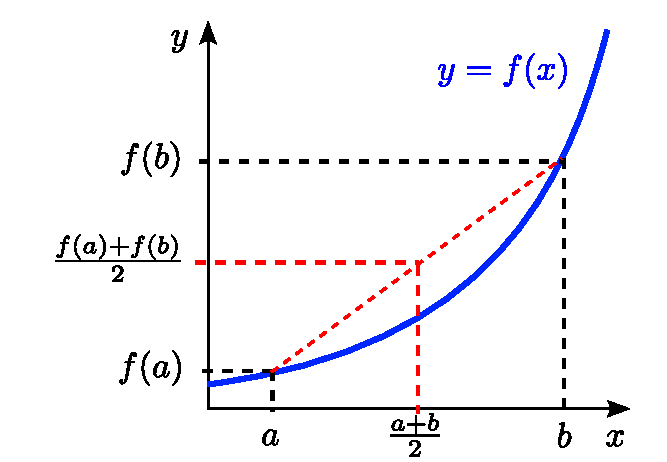
\includegraphics[width=0.45\linewidth]{Appendix1/jensen_discrete.pdf}}
 \hfill
 \subfigure[for continuous distributions]{
 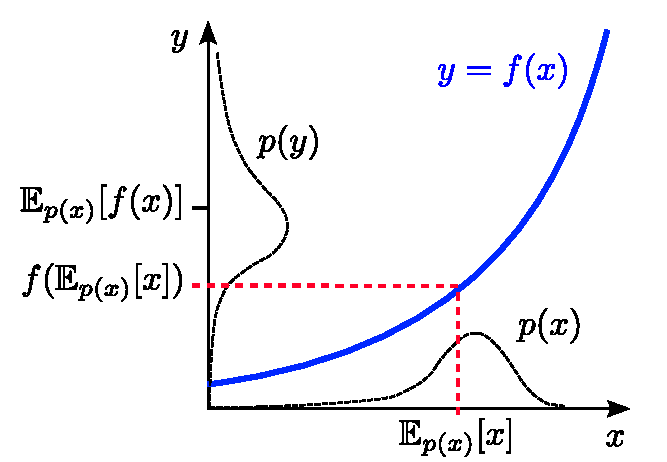
\includegraphics[width=0.45\linewidth]{Appendix1/jensen.pdf}}
 \caption{A visual proof of the Jensen's inequality. }
 \label{fig:appendix_jensen}
\end{figure}


\subsection{H{\"o}lder's inequality}
\begin{prop}
(H{\"o}lder's Inequality)
Let $(\mathcal{X}, \Sigma, \mu)$ be a measure space and let $p, q \in [1, +\infty]$ satisfying $\frac{1}{p} + \frac{1}{q} = 1$, then for all measurable functions $f$, $g$ on $\mathcal{X}$,
$$ \int | f(x) g(x) | d \mu \leq \left( \int | f(x) |^p d \mu \right)^{\frac{1}{p}} \left( \int | g(x) |^q d \mu \right)^{\frac{1}{q}} .$$
\end{prop}
Setting $p = q = 2$ recovers the Cauchy-Schwarz inequality.
%
\begin{proof}
We assume $\exists x \in \mathcal{X} \text{ s.t. } f(x) \neq 0$ w.l.o.g., then
\begin{equation*}
\begin{aligned}
 \int | f(x) g(x) | d \mu &= \left( \int | f(x) |^p d \mu \right) \int [ ( | g(x) | | f(x) |^{1 - p} )^{q} ]^{\frac{1}{q}} \frac{|f(x)|^p}{ \int | f(x) |^p d \mu } d \mu \\
 &\leq \left( \int | f(x) |^p d \mu \right) \left[ \int ( | g(x) | | f(x) |^{1 - p} )^{q} \frac{|f(x)|^p}{ \int | f(x) |^p d \mu } d \mu \right]^{\frac{1}{q}} \\
 &= \left( \int | f(x) |^p d \mu \right)^{1 - \frac{1}{q}} \left[ \int | g(x) |^{q} d \mu \right]^{\frac{1}{q}} \\
 &= \left( \int | f(x) |^p d \mu \right)^{\frac{1}{p}} \left[ \int | g(x) |^{q} d \mu \right]^{\frac{1}{q}}.
\end{aligned}
\end{equation*}
For the second line we used the Jensen's inequality, with the function $h(x) = x^{\frac{1}{q}}$ which is convex when $q >= 1$, and the probability measure $p(x) = \frac{|f(x)|^p}{ \int | f(x) |^p d \mu }$. For the third and the last lines we used the assumption that $\frac{1}{p} + \frac{1}{q} = 1$.
\end{proof}

\subsection{Stein's identity}
We provide a proof of Stein's identity in 1D case. The general case can be proved accordingly.
\begin{prop}
(Stein's identity, one dimensional case)
Let $p(x)$ be a differentiable probability density function of $x \in \mathbb{R}$. Let $h(x)$ be a function such that $\lim_{x \rightarrow \pm \infty} p(x) h(x) = 0$. Then
$$\mathbb{E}_{p}[h(x) \nabla_{x} \log p(x) + \nabla_{x} h(x) ] = 0 .$$ 
\end{prop}

\begin{proof}
Using integration by parts, we have
\begin{equation*}
\begin{aligned}
\mathbb{E}_{p}[h(x) \nabla_{x} \log p(x) + \nabla_{x} h(x) ] &= \int p(x) h(x) \nabla_{x} \log p(x) dx + \int p(x) \nabla_{x} h(x) dx \\
&= \int h(x) \nabla_{x} p(x) dx + \int p(x) \nabla_{x} h(x) dx \\
&= \int \nabla_{x} [h(x) p(x)] dx \\
&= h(x) p(x) |_{-\infty}^{+\infty} = 0. \quad\quad \text{// boundary condition}
\end{aligned}
\end{equation*}
\end{proof}

\cite{stein:stein_method1972} proposed the following lemma for Gaussian distribution.
\begin{lemma}
(\citep{stein:stein_method1972})
Let $p(x) = \mathcal{N}(x; \mu, \sigma^2)$, and the function $h(x)$ satisfies $| \mathbb{E}_{p}[g(x) (x - \mu)] |< +\infty$ and $|\mathbb{E}_{p}[\nabla_{x} g(x)] | < +\infty$. Then
$$ \mathbb{E}_{p}[g(x) (x - \mu)] = \sigma^2 \mathbb{E}_p[\nabla_{x} g(x)]. $$
\end{lemma}

Later, \cite{chen:poisson1975} extended the characterisation to Poisson distribution.
\begin{lemma}
(\citep{chen:poisson1975}) A random variable $x$ taking values in $\mathbb{N}$ is Poisson distributed with rate $\lambda$, if and only if $P(x)$ satisfies
$$ \mathbb{E}_{P}[ \lambda h(x+1) - xh(x) ] = 0 $$
for all bounded functions $h: \mathbb{N} \rightarrow \mathbb{R}$.
\end{lemma}
\begin{proof}
Assume $x$ is Poisson distributed with rate $\lambda$, then
\begin{equation*}
\begin{aligned}
\mathbb{E}_{P}[ \lambda h(x+1) - xh(x) ] 
& = \sum_{n=0}^{+\infty} \lambda h(n+1) \exp[-\lambda] \frac{\lambda^n}{n!} - \sum_{n=0}^{+\infty} n h(n) \exp[-\lambda] \frac{\lambda^n}{n!} \\
& = \sum_{n=1}^{+\infty} h(n) \exp[-\lambda] \frac{\lambda^n}{(n-1)!} - \sum_{n=1}^{+\infty} h(n) \exp[-\lambda] \frac{\lambda^n}{(n - 1)!} = 0. \\
\end{aligned}
\end{equation*}
Conversely if the identity holds for every function $h(x)$, then setting $h(x) = \delta_{x - k}$ for some $k$, by assumption we have
$$ \mathbb{E}_{P}[ \lambda h(x+1) - xh(x) ] = \lambda P(x = k - 1) - k P(k) = 0,$$
which implies 
$$ \frac{P(x = k)}{P(x = k-1)} = \frac{\lambda}{k} = \frac{\text{Poisson}_{\lambda}( x = k)}{ \text{Poisson}_{\lambda}( x = k - 1) }.$$
Since it holds for all $k \in \mathbb{N}^{+}$, we conclude that $x$ is Poisson distributed.
\end{proof}


\end{appendices}

% *************************************** Index ********************************
\printthesisindex % If index is present

\end{document}
